\documentclass[krantz1]{krantz} %See documentation for other class options
\usepackage{fixltx2e,fix-cm}
\usepackage{amssymb}
\usepackage{amsmath, bm}
\usepackage{graphicx}
\usepackage{subfigure}
\usepackage{makeidx}
\usepackage{multicol}
\usepackage{listings}
\usepackage{bbm}
\usepackage[skins]{tcolorbox}
\usepackage{enumitem}
%\usepackage[dvips]{hyperref}

%%%%%%%%%%%%%%%%%%%%%%%%%%%%%%%%%%
\usepackage{listings}
\usepackage{xcolor}

\definecolor{codegreen}{rgb}{0,0.6,0}
\definecolor{codegray}{rgb}{0.5,0.5,0.5}
\definecolor{codepurple}{rgb}{0.58,0,0.82}
\definecolor{backcolour}{rgb}{0.95,0.95,0.92}

\lstdefinestyle{mystyle}{
	backgroundcolor=\color{backcolour},   
	commentstyle=\color{codegreen},
	keywordstyle=\color{magenta},
	numberstyle=\tiny\color{codegray},
	stringstyle=\color{codepurple},
	basicstyle=\ttfamily\footnotesize,
	breakatwhitespace=false,         
	breaklines=true,    captionpos=b,                    
	keepspaces=true, numbers=left,                    
	numbersep=5pt, showspaces=false,                
	showstringspaces=false, showtabs=false, tabsize=2}
\lstset{style=mystyle}
%%%%%%%%%%%%%%%%%%%%%%%%%%%%%%%%%%%%%%%%%%%%%


\makeindex

\usepackage{booktabs}
 %place custom commands and macros here

\begin{document}

\frontmatter

\title{Krantz Template} %This is a placeholder titlepage, it will not be final.
\author{Yours Truly}
%%%\maketitle

%%%Placeholder for front matter

\halftitle{\Large{\noindent Solution Manual\\
		Introduction to Bayesian Inference:\\
		A GUIded tour using R}}


\booktitle{\Large{\noindent Solution Manual\\
		Introduction to Bayesian Inference:\\
		A GUIded tour using R\\
		
		by Andrés Ramírez-Hassan, PhD. Statistical Science.}}

% \locpage

\cleardoublepage
\thispagestyle{empty}
\vspace*{\stretch{1}}
\begin{center}
\Large\itshape
To my parents, Nancy and Orlando.
\end{center}
\vspace{\stretch{2}}
\cleardoublepage
\setcounter{page}{7} %previous pages will be reserved for frontmatter to be added in later.
\tableofcontents
\chapter*{Foreword}
I am delighted to introduce the first book on Multimedia Data Mining.  When I came to know about this book project undertaken by two of the most active young researchers in the field, I was pleased that this book is coming in early stage of a field that will need it more than most fields do.  In most emerging research fields, a book can play a significant role in bringing some maturity to the field.  Research fields advance through research papers.  In research papers, however, only a limited perspective could be provided about the field, its application potential, and the techniques required and already developed in the field.  A book gives such a chance.  I liked the idea that there will be a book that will try to unify the field by bringing in disparate topics already available in several papers that are not easy to find and understand.  I was supportive of this book project even before I had seen any material on it.  The project was a brilliant and a bold idea by two active researchers.  Now that I have it on my screen, it appears to be even a better idea.  

Multimedia started gaining recognition in 1990s as a field.  Processing, storage, communication, and capture and display technologies had advanced enough that researchers and technologists started building approaches to combine information in multiple types of signals such as audio, images, video, and  text.  Multimedia computing and communication techniques recognize correlated information in multiple sources as well as insufficiency of information in any individual source.    By properly selecting sources to provide complementary information, such systems aspire, much like human perception system, to create a holistic picture of a situation using only partial information from separate sources.

Data mining is a direct outgrowth of progress in data storage and processing speeds.  When it became possible to store large volume of data and run different statistical computations to explore all possible and even unlikely correlations among data, the field of data mining was born.  Data mining allowed people to hypothesize relationships among data entities and explore support for those.  This field has been put to applications in many diverse domains and keeps getting more applications.  In fact many new fields are direct outgrowth of data mining and it is likely to become a powerful computational tool.\vadjust{\vfill\pagebreak}



\chapter*{Preface}
The main goal of this book is to make the Bayesian inferential framework more approachable to students, researchers, and practitioners who wish to understand and apply this statistical/econometric approach but do not have the time to develop programming skills. I have aimed to strike a balance between applicability and theory. This book provides a very user-friendly graphical user interface (GUI) to implement the most common regression models, while also covering the basic mathematical developments and their code implementation for those interested in advancing to more complex models.

\textbf{To instructors and students}

This book is divided into three parts: foundations (chapters 1 to 4), regression analysis (chapters 5 to 10), and \textit{Advanced} methods (chapters 11 to 14). Our graphical user interface (GUI) is designed for the second part. The source code can be found at \textbf{https://github.com/besmarter/BSTApp}. Instructors and students can access all the code, along with simulated and real datasets. There are three ways to install our GUI:

\begin{enumerate}
	\item Type \textbf{shiny::runGitHub(``besmarter/BSTApp", launch.browser=T)} in the \textbf{R} console or any \textbf{R} code editor and execute it.
	\item Visit \textbf{https://posit.cloud/content/4328505}, log in or sign up for \textbf{Posit Cloud}, navigate to the \textbf{BSTApp-master} folder in the \textbf{Files} tab of the right-bottom window, then click on the \textbf{app.R} file and select \textbf{Run App}.
	\item Use a \textbf{Docker} image by typing in the \textbf{Command Prompt}
	\begin{enumerate}
		\item docker pull magralo95/besmartergui:latest
		\item docker run --rm -p 3838:3838 magralo95/besmartergui
	\end{enumerate}
	Then users can access our GUI going to \textbf{http://localhost:3838/}. See Chapter \ref{chapGUI} for details.
\end{enumerate}

Students should have a basic understanding of probability theory and statistics, as well as some background in econometrics and time series, particularly regression analysis. Familiarity with standard univariate and multivariate probability distributions is strongly recommended. See a nice summary of useful probability distributions in \cite[p.~182-191]{greenberg2012introduction}. Additionally, students who wish to master the material in this book should have programming skills in \textbf{R} software.\footnote{An excellent starting point for \textbf{R} programming is the \textit{R Introduction Manual}: \textbf{https://cran.r-project.org/doc/manuals/r-release/R-intro.pdf}.}


I have included both formal and computational exercises at the end of each chapter to help students gain a better understanding of the material presented. A solutions manual for these exercises accompanies this book.

Instructors can use this book as a textbook for a course on introductory Bayesian Econometrics/Statistics, with a strong emphasis on implementation and applications. This book is intended to be complementary, rather than a substitute, for excellent resources on the topic, such as \cite{gelman2021bayesian}, \cite{chan2019bayesian}, \cite{rossi2012bayesian}, \cite{greenberg2012introduction}, \cite{geweke2005contemporary}, \cite{lancaster2004introduction}, and \cite{koop2003bayesian}.


\textbf{Acknowledgments}

I began developing our graphical user interface (GUI) in 2016, after being diagnosed with cervical dystonia. I worked on this side project during weekends, which I called ``nerd weekends,'' and it served as a form of release from my health condition. Once I began to recover, I invited Mateo Graciano, my former student, business partner, and friend, to join the project. He has been instrumental in developing our GUI, and I am enormously grateful to him. 

I would also like to thank the members of the BEsmarter research group at Universidad EAFIT, as well as the NUMBATs members at Monash University, for their valuable feedback and recommendations to improve our GUI.

This book is an extension of the paper \textit{A GUIded tour of Bayesian regression} \cite{Ramirez2020}, which serves as a brief user guide for our GUI. I decided to write this book to explain the underlying theory and code in our GUI, and to use it as a textbook in my course on Bayesian econometrics/statistics. I am grateful to my students in this course; their insights and thoughtful questions have deepened my understanding of the material.

I would like to thank Chris Parmeter for his valuable suggestions on how to present our user guide; Professors Raúl Pericchi and Juan Carlos Correa for introducing me to Bayesian statistics; and Liana Jacobi, Tomasz Wozniak, and Chun Fung Kwok (Jackson) from the University of Melbourne, as well as David Frazier from Monash University, for their engaging discussions and fruitful collaborations in Bayesian econometrics and statistics. I am also deeply grateful to Professor Peter Diggle for his unwavering support of my career, and especially to Professor Gael Martin, who gave me the opportunity to work with her and has been a constant source of intellectual inspiration.  

I also wish to acknowledge my colleagues and staff at Universidad EAFIT for their continuous support.  

Finally, I acknowledge the use of ChatGPT, which assisted me in improving the grammar, clarity, and flow of the text, as well as in tidying up the code presented in this book. Nevertheless, all concepts, mathematical developments, and underlying logic are entirely my own, based on my understanding and readings of the literature. Any remaining errors are solely my responsibility, for which I apologize in advance. I sincerely thank the reader and hope that this book proves useful.  

To my parents, Orlando and Nancy, who have always been there for me with their unconditional support. They have taught me that the primary aspect of human spiritual evolution is humility, a lesson I am still learning every day. To my fiancée, Estephania, for her unwavering love and support.





%%\listoffigures
%%\listoftables
%%%\twocolumn
\chapter*{Contributors}

\begin{multicols}{2}
\contributor{Michael Aftosmis}{NASA Ames Research Center}{Moffett Field, California}

\contributor{Pratul K. Agarwal}{Oak Ridge National Laboratory}{Oak Ridge, Tennessee}

\contributor{Sadaf R. Alam}{Oak Ridge National Laboratory}{Oak Ridge, Tennessee}

\contributor{Gabrielle Allen}{Louisiana State University}{Baton Rouge, Louisiana}

\contributor{Martin Sandve Aln{\ae}s}{Simula Research Laboratory and University of Oslo, Norway}{Norway}

\contributor{Steven F. Ashby} {Lawrence Livermore National Laboratory}{Livermore, California}

\contributor{David A. Bader} {Georgia Institute of Technology}{Atlanta, Georgia}

\contributor{Benjamin Bergen} {Los Alamos National Laboratory}{Los Alamos, New Mexico}

\contributor{Jonathan W. Berry} {Sandia National Laboratories}{Albuquerque, New Mexico}

\contributor{Martin Berzins}{University of Utah}{Salt Lake City, Utah}

\contributor{Abhinav Bhatele}{University of Illinois}{Urbana-Champaign, Illinois}

\contributor{Christian Bischof} {RWTH Aachen University}{Germany}

\contributor{Rupak Biswas} {NASA Ames Research Center}{Moffett Field, California}\vspace*{5pt}

\contributor{Eric Bohm} {University of Illinois}{Urbana-Champaign, Illinois}\vspace*{5pt}

\contributor{James Bordner} {University of California, San Diego}{San Diego, California}\vspace*{5pt}

\contributor{George Bosilca} {University of Tennessee}{Knoxville, Tennessee}\vspace*{5pt}

\contributor{Greg L. Bryan} {Columbia University}{New York, New York}\vspace*{5pt}

\contributor{Marian Bubak} {AGH University of Science and Technology}{
Krak{\'o}w, Poland}\vspace*{5pt}

\contributor{Andrew Canning}{Lawrence Berkeley National
Laboratory}{Berkeley, California}

\contributor{Jonathan Carter} {Lawrence Berkeley National
Laboratory}{Berkeley, California}

\contributor{Zizhong Chen} {Jacksonville State University}{Jacksonville,
Alabama}

\contributor{Joseph R. Crobak} {Rutgers, The State University of New
Jersey}{Piscataway, New Jersey}

\contributor{Roxana E. Diaconescu} {Yahoo! Inc.}{Burbank, California}

\contributor{Peter Diener}
{Louisiana State University}{Baton Rouge, Louisiana}

\contributor{Jack J. Dongarra} {University of Tennessee, Knoxville, 
Oak Ridge National Laboratory, and}{University of Manchester}

\contributor{John B. Drake} {Oak Ridge National Laboratory}{Oak Ridge,
Tennessee}

\contributor{Kelvin K. Droegemeier} {University of Oklahoma}{Norman,
Oklahoma}

\contributor{St{\'e}phane Ethier} {Princeton University}{Princeton, New
Jersey}

\contributor{Christoph Freundl}
{Friedrich--Alexander--Universit{\"a}t}{Erlangen, Germany}

\contributor{Karl F{\"u}rlinger} {University of Tennessee}{Knoxville,
Tennessee}

\contributor{Al Geist} {Oak Ridge National Laboratory}{Oak Ridge,
Tennessee}

\contributor{Michael Gerndt} {Technische Universit{\"a}t
M{\"u}nchen}{Munich, Germany}

\contributor{Tom Goodale}
{Louisiana State University}{Baton Rouge, Louisiana}

\contributor{Tobias Gradl}
{Friedrich--Alexander--Universit{\"a}t}{Erlangen, Germany}

\contributor{William D. Gropp} {Argonne National Laboratory}{Argonne,
Illinois}

\contributor{Robert Harkness} {University of California, San
Diego}{San Diego, California}

\contributor{Albert Hartono} {Ohio State University}{Columbus, Ohio}

\contributor{Thomas C. Henderson} {University of Utah}{Salt Lake City,
Utah}

\contributor{Bruce A. Hendrickson} {Sandia National
Laboratories}{Albuquerque, New Mexico}

\contributor{Alfons G. Hoekstra} {University of Amsterdam}{Amsterdam,
The Netherlands}

\contributor{Philip W. Jones} {Los Alamos National Laboratory}{Los
Alamos, New Mexico}

\contributor{Laxmikant Kal{\'e}} {University of
Illinois}{Urbana-Champaign, Illinois}

\contributor{Shoaib Kamil} {Lawrence Berkeley National
Laboratory}{Berkeley, California}

\contributor{Cetin Kiris} {NASA Ames Research Center}{Moffett Field,
California}

\contributor{Uwe K{\"u}ster} {University of Stuttgart}{Stuttgart,
Germany}

\contributor{Julien Langou} {University of Colorado}{Denver, Colorado}

\contributor{Hans Petter Langtangen}
{Simula Research Laboratory and}{University of Oslo, Norway}

\contributor{Michael Lijewski} {Lawrence Berkeley National
Laboratory}{Berkeley, California}

\contributor{Anders Logg}
{Simula Research Laboratory and}{University of Oslo, Norway}

\contributor{Justin Luitjens} {University of Utah}{Salt Lake City, Utah}

\contributor{Kamesh Madduri} {Georgia Institute of Technology}{Atlanta,
Georgia}

\contributor{Kent-Andre Mardal}
{Simula Research Laboratory and}{University of Oslo, Norway}

\contributor{Satoshi Matsuoka} {Tokyo Institute of Technology}{Tokyo,
Japan}

\contributor{John M. May} {Lawrence Livermore National
Laboratory}{Livermore, California}

\contributor{Celso L. Mendes} {University of Illinois}{Urbana-Champaign,
Illinois}

\contributor{Dieter an Mey} {RWTH Aachen University}{Germany}

\contributor{Tetsu Narumi} {Keio University}{Japan}

\contributor{Michael L. Norman} {University of California, San
Diego}{San Diego, California}

\contributor{Boyana Norris} {Argonne National Laboratory}{Argonne,
Illinois}

\contributor{Yousuke Ohno} {Institute of Physical and Chemical Research
(RIKEN)}{Kanagawa, Japan}

\contributor{Leonid Oliker} {Lawrence Berkeley National
Laboratory}{Berkeley, California}

\contributor{Brian O'Shea} {Los Alamos National Laboratory}{Los Alamos,
New Mexico}

\contributor{Christian D. Ott}
{University of Arizona}{Tucson, Arizona}

\contributor{James C. Phillips} {University of
Illinois}{Urbana-Champaign, Illinois}

\contributor{Simon Portegies Zwart} {University of
Amsterdam,}{Amsterdam, The Netherlands}

\contributor{Thomas Radke}
{Albert-Einstein-Institut}{Golm, Germany}

\contributor{Michael Resch} {University of Stuttgart}{Stuttgart,
Germany}

\contributor{Daniel Reynolds} {University of California, San Diego}{San
Diego, California}

\contributor{Ulrich R{\"u}de}
{Friedrich--Alexander--Universit{\"a}t}{Erlangen, Germany}

\contributor{Samuel Sarholz}
{RWTH Aachen University}{Germany}

\contributor{Erik Schnetter}
{Louisiana State University}{Baton Rouge, Louisiana}

\contributor{Klaus Schulten} {University of Illinois}{Urbana-Champaign,
Illinois}

\contributor{Edward Seidel}
{Louisiana State University}{Baton Rouge, Louisiana}

\contributor{John Shalf} {Lawrence Berkeley National
Laboratory}{Berkeley, California}

\contributor{Bo-Wen Shen} {NASA Goddard Space Flight Center}{Greenbelt,
Maryland}

\contributor{Ola Skavhaug}
{Simula Research Laboratory and}{University of Oslo, Norway}

\contributor{Peter M.A. Sloot} {University of Amsterdam}{Amsterdam, The
Netherlands}

\contributor{Erich Strohmaier} {Lawrence Berkeley National
Laboratory}{Berkeley, California}

\contributor{Makoto Taiji} {Institute of Physical and Chemical Research
(RIKEN)}{Kanagawa, Japan}

\contributor{Christian Terboven}
{RWTH Aachen University,}{Germany}

\contributor{Mariana Vertenstein} {National Center for Atmospheric
Research}{Boulder, Colorado}

\contributor{Rick Wagner} {University of California, San Diego}{San
Diego, California}

\contributor{Daniel Weber} {University of Oklahoma}{Norman, Oklahoma}

\contributor{James B. White, III} {Oak Ridge National Laboratory}{Oak
Ridge, Tennessee}

\contributor{Terry Wilmarth} {University of Illinois}{Urbana-Champaign,
Illinois}

\end{multicols}
\chapter*{Symbols}
\begin{symbollist}{000000}
\symbolentry{$\lnot$}{Negation symbol.}
\symbolentry{$\propto$}{Proportional symbol.}
\symbolentry{$\perp$}{Independence symbol.}
\symbolentry{$\mathcal{R}$}{The Real set.}
\symbolentry{$\emptyset$}{Empty set.}
\symbolentry{$\mathbbm{1}$}{Indicator function.}


\end{symbollist}

\mainmatter

\part{Foundations: Theory, simulation methods and programming}
\chapter{Basic formal concepts}\label{chap1}

We introduce formal concepts in Bayesian inference starting with the Bayes’ rule, all its components with their formal definitions and basic examples. In addition, we present some nice features of Bayesian inference such as Bayesian updating, and asymptotic sampling properties, and the basics of Bayesian inference based on decision theory under uncertainty, presenting important concepts like loss function, risk function and optimal rules.

\section{The Bayes' rule}\label{sec11}
As expected the point of departure to perform Bayesian inference is the Bayes' rule,\footnote{Observe that I use the term ``Bayes' rule" rather than ``Bayes' theorem". It was Laplace \cite{laplace1774memoire} who actually generalized the Bayes' theorem \cite{bayes1763lii}. His generalization is named the Bayes' rule.} which is the Bayes' solution to the inverse probability of causes, this rule combines prior beliefs with objective probabilities based on repeatable experiments. In this way, we can move from observations to probable causes. 

Formally, the conditional probability of $A_i$ given $B$ is equal to the conditional probability of $B$ given $A_i$ times the marginal probability of $A_i$ over the marginal probability of $B$,

\begin{align}
	P(A_i|B)&=\frac{P(A_i,B)}{P(B)}\nonumber\\
	&=\frac{P(B|A_i) \times P(A_i)}{P(B)},
	\label{eq:111}
\end{align}

where by the law of total probability $P(B)=\sum_i P(B|A_i)P(A_i)\neq 0$, $\left\{A_i, i=1,2,\dots\right\}$ is a finite or countably infinite partition of a sample space.

In the Bayesian framework, $B$ is sample information that updates a probabilistic statement about an unknown object $A_i$ following probability rules. This is done by means of the Bayes' rule using prior ``beliefs" about $A_i$, that is, $P(A_i)$, sample information relating $B$ to the particular state of the nature $A_i$ through a probabilistic statement, $P(B|A_i)$, and the probability of observing that specific sample information $P(B)$.  

Let's see a simple example, \textit{the base rate fallacy}:

Assume that the sample information comes from a positive result from a test whose true positive rate (sensitivity) is 98\%, $P(+|\text{disease})=0.98$. On the other hand, the prior information regarding being infected with this disease comes from a base incidence rate that is equal to 0.002, that is $P(\text{disease})=0.002$. Then, \textit{what is the probability of being actually infected?}

This is an example of \textit{the base rate fallacy}, where having a positive test result from a disease whose base incidence rate is tiny gives a low probability of actually having the disease.

The key to answer the question is based on understanding the difference between the probability of having the disease given a positive result, $P(\text{disease}|+)$, versus the probability of a positive result given the disease, $P(+|\text{disease})$. The former is the important result, and the Bayes' rule help us to get the answer. Using the Bayes' rule (equation \ref{eq:111}):

\begin{align*}
	P(\text{disease}|+) & = \frac{P(+|\text{disease})\times P(\text{disease})}{P(+)}\\
	& = \frac{0.98 \times 0.002}{0.98 \times 0.002 + (1-0.98) \times (1-0.002)}\\
	& =0.09, 
\end{align*}

where $P(+)=P(+|\text{disease})\times P(\text{disease})+P(+|\lnot\text{disease})\times P( \lnot\text{disease})$.\footnote{$\lnot$ is the negation symbol. In addition, we have that $P(B|A)=1-P(B|A^c)$ in this example, where $A^c$ is the complement of $A$. However, it is not always the case that $P(B|A)\neq 1-P(B|A^c)$.}

\begin{tcolorbox}[enhanced,width=4.67in,center upper,
	fontupper=\large\bfseries,drop shadow southwest,sharp corners]
\textit{R code. The base rate fallacy}
\begin{VF}
\begin{lstlisting}[ language=R]
PD <- 0.002 # Probability of disease
PPD <- 0.98 # True positive (Sensitivity)
PDP <- PD * PPD / (PD * PPD + (1 - PD)*(1 - PPD))
paste("Probability of disease given a positive test is", sep = " ", round(PDP, 2))
"Probability of disease given a positive test is 0.09"
\end{lstlisting}
\end{VF}
\end{tcolorbox}

We observe that despite of having a positive result, the probability of having the disease is low. This due to the base rate being tiny.

Another interesting example, which is at the heart of the origin of the Bayes' theorem \cite{bayes1763lii}, is related to the existence of God \cite{stigler2018richard}. The Section X of David Hume's ``An Inquiry concerning Human Understanding, 1748" is named \textit{Of Miracles}. There, Hume argues that when someone claims to have seen a miracle, this is poor evidence it actually happened, since it goes against what we see every day. Then, Richard Price, who actually finished and published ``An essay towards solving a problem in the doctrine of chances" in 1763 after Bayes died in 1761, argues against Hume saying that there is a huge difference between \textit{impossibility} as used commonly in conversation and \textit{physical impossibility}. Price used an example of a dice with a million sides, where \textit{impossibility} is getting a particular side when throwing this dice, and \textit{physical impossibility} is getting a side that does not exist. In millions throws, the latter case never would occur, but the former eventually would.

Let's say that there are two cases of resurrection (Res), Jesus Christ and Elvis, and the total number of people who have ever lived is 108.5 billion,\footnote{https://www.wolframalpha.com/input/?i=number+of+people+who+have+ever+lived+on+Earth} then the prior base rate is $2/(108.5\times 10^{9})$. On the other hand, let's say that the sample information comes from a very reliable witness whose true positive rate is  0.9999999. Then, \textit{what is the probability of this miracle?}\footnote{https://www.r-bloggers.com/2019/04/base-rate-fallacy-or-why-no-one-is-justified-to-believe-that-jesus-rose/}

Using the Bayes' rule:
{\small{
\begin{align*}
	P(\text{Res}|\text{Witness}) & =  \frac{P(\text{Witness}|\text{Res})\times P(\text{Res})}{P(\text{Witness})}\\
	& =\frac{2/(108.5 * 10^9) \times 0.9999999}{2/(108.5 * 10^9) \times 0.9999999 + (1-2/(108.5 * 10^9)) \times (1-0.9999999)}\\
	& = 0.000184297806959661
\end{align*}
}}

where $P(\text{Witness})=P(\text{Witness}|\text{Res})\times P(\text{Res})+(1-P(\text{Witness}|\text{Res}))\times (1-P(\text{Res}))$.

Thus, $1.843\times 10^{-4}$ is the probability of a resurrection given a very reliable witness.

\begin{tcolorbox}[enhanced,width=4.67in,center upper,
	fontupper=\large\bfseries,drop shadow southwest,sharp corners]
\textit{R code. Of Miracles}
\begin{VF}
\begin{lstlisting}[ language=R]
# Probability of resurrection
PR <- 2/(108.5 * 10^9) 
PWR <- 0.9999999 # True positive rate
PRW <- PR * PWR / (PR * PWR + (1 - PR)*(1 - PWR)) 
paste("Probability of resurrection given witness is", sep = " ", PRW)
"Probability of resurrection given witness is 0.000184297806959661"
\end{lstlisting}
\end{VF}
\end{tcolorbox}

Observe that we can condition on many events in the Bayes' rule. Let's have two conditioning events $B$ and $C$, then equation \ref{eq:111} becomes

\begin{align}
	P(A_i|B,C)&=\frac{P(A_i,B,C)}{P(B,C)}\nonumber\\
	&=\frac{P(B|A_i,C) \times P(A_i|C) \times P(C)}{P(B|C)P(C)}.
	\label{eq:112}
\end{align}

Let's use this rule in one of the most intriguing statistical puzzles, \textit{the Monty Hall problem}, to illustrate how to use equation \ref{eq:112} \cite{selvin1975problem,selvin1975bproblem}. This was the situation faced by a contestant in the American television game show \textit{Let's Make a Deal}. There, the contestant was asked to choose a door where behind one door there is a car, and behind the others, goats. Let's say that the contestant picks door No. 1, and the host (Monty Hall), who knows what is behind each door, opens door No. 3, where there is a goat (see Figure \ref{fig11}). Then, the host asks the tricky question to the contestant, \textit{do you want to pick door No. 2?}

\begin{figure}
	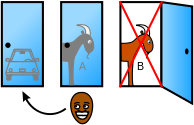
\includegraphics[width=340pt, height=200pt]{Chapters/chapter1/figures/MHproblem.png}
	%%\centerline{\epsfig{/Chapters/chapter1/figures/cat.eps,width=.8\textheight,height=.4\textwidth}}
	\caption[List of figure caption goes here]{The Monty Hall problem.}\label{fig11}
\end{figure}

Let's name $P_i$ the event \textbf{contestant picks door No. $i$}, which stays close, $H_i$ the event \textbf{host picks door No. $i$}, which is open, and there is a goat, and $C_i$ the event \textbf{car is behind door No. $i$}. In this particular setting, the contestant is interested in the probability of the event $P(C_2|H_3,P_1)$. A naive answer would be that it is irrelevant as initially $P(C_i)=1/3, \ i=1,2,3$, and now $P(C_i|H_3)=1/2, \ i=1,2$ as the host opened door No. 3. So, why bothering changing the initial guess if the odds are the same (1:1)? The important point here is that the host knows what is behind each door, and picks a door where there is a goat given contestant choice. In this particular setting, $P(H_3|C_3,P_1)=0$, $P(H_3|C_2,P_1)=1$ and $P(H_3|C_1,P_1)=1/2$. Then, using equation \ref{eq:112} 

\begin{align*}
	P(C_2|H_3,P_1)&= \frac{P(C_2,H_3,P_1)}{P(H_3,P_1)}\\
	&= \frac{P(H_3|C_2,P_1)P(C_2|P_1)P(P_1)}{P(H_3|P_1)\times P(P_1)}\\
	&= \frac{P(H_3|C_2,P_1)P(C_2)}{P(H_3|P_1)}\\
	&=\frac{1\times 1/3}{1/2},
\end{align*}
where the third equation uses the fact that $C_i$ and $P_i$ are independent events, and $P(H_3|P_1)=1/2$ due to this depending just on $P_1$ (not on $C_2$).

Therefore, changing the initial decision increases the probability of getting the car from 1/3 to 2/3! Thus, it is always a good idea to change the door.

Let's see a simulation exercise to check this answer:

\begin{tcolorbox}[enhanced,width=4.67in,center upper,
	fontupper=\large\bfseries,drop shadow southwest,sharp corners]
\textit{R code. The Monty Hall problem}
\begin{VF}
\begin{lstlisting}[ language=R]
set.seed(0101) # Set simulation seed
S <- 100000 # Simulations
Game <- function(switch = 0){
	# switch = 0 is not change  
	# switch = 1 is to change
	opts <- 1:3 
	car <- sample(opts, 1) # car location
	guess1 <- sample(opts, 1) # Initial guess 
	
	if(car != guess1) {
	 host <- opts[-c(car, guess1)]
	} else {
	 host <- sample(opts[-c(car, guess1)], 1)
	}	
	win1 <- guess1 == car # Win no change
	guess2 <- opts[-c(host, guess1)]	
	win2 <- guess2 == car # Win change
	if(switch == 0){
		win <- win1
	} else {
		win <- win2
	}
	return(win)
}

#Win probabilities not changing
Prob <- mean(replicate(S, Game(switch = 0))) 
Prob
0.3334

#Win probabilities changing
Prob <- mean(replicate(S, Game(switch = 1))) 
Prob
0.6654
\end{lstlisting}
\end{VF}
\end{tcolorbox}

\section{Bayesian framework: A brief summary of theory}\label{sec12}

For two random objects $\bm{\theta}$ and $\mathbf{y}$, the Bayes' rule may be analogously used,\footnote{From a Bayesian perspective $\mathbf{\theta}$ is fixed, but unknown. Then, it is treated as a random object despite the lack of variability (see Chapter \ref{chap2}).}

\begin{align}
	\pi(\bm{\theta}|\mathbf{y})&=\frac{p(\mathbf{y}|\bm{\theta}) \times \pi(\bm{\theta})}{p(\mathbf{y})},
	\label{eq:121}
\end{align}

where $\pi(\bm{\theta}|\mathbf{y})$ is the posterior density function, $\pi(\bm{\theta})$ is the prior density, $p(\mathbf{y}|\bm{\theta})$ is the likelihood (statistical model), and

\begin{equation}
	p(\mathbf{y})=\int_{\mathbf{\Theta}}p(\mathbf{y}|\bm{\theta})\pi(\bm{\theta})d\bm{\theta}=\mathbb{E}\left[p(\mathbf{y}|\bm{\theta})\right]
	\label{eq:121a}
\end{equation}

is the marginal likelihood or prior predictive. Observe that for this expected value to be meaningful the prior should be a proper density, that is, integrates to one, otherwise, it does not make sense. 

Observe that $p(\mathbf{y}|\bm{\theta})$ is not a density in $\bm{\theta}$. In addition, $\pi(\bm{\theta})$ does not have to integrate to 1, that is, $\pi(\bm{\theta})$ can be an improper density function, $\int_{\mathbf{\Theta}}\pi(\bm{\theta})d\bm{\theta}=\infty$. However, $\pi(\bm{\theta}|\mathbf{y})$ is a proper density function, that is, $\int_{\mathbf{\Theta}}\pi(\bm{\theta}|\mathbf{y})d\bm{\theta}=1$. For instance, set $\pi(\bm{\theta})=c$, where $c$ is a constant, then $\int_{\mathbf{\Theta}}cd\bm{\theta}=\infty$. However, $\int_{\mathbf{\Theta}}\pi(\bm{\theta}|\mathbf{y})d\bm{\theta}=\int_{\mathbf{\Theta}}\frac{p(\mathbf{y}|\bm{\theta})\times c}{\int_{\mathbf{\Theta}} p(\mathbf{y}|\bm{\theta})\times c d\bm{\theta}}d\bm{\theta}=1$ where $c$ cancels out.  

$\pi(\bm{\theta}|\mathbf{y})$ is a sample updated ``probabilistic belief" version of $\pi(\bm{\theta})$, where $\pi(\bm{\theta})$ is a prior probabilistic belief which can be constructed from previous empirical work, theory foundations, expert knowledge and/or mathematical convenience. This prior usually depends on parameters, which are named \textit{hyperparameters}. In addition, the Bayesian approach implies using a probabilistic model about $\mathbf{y}$ given $\bm{\theta}$, that is, $p(\mathbf{y}|\bm{\theta})$, where its integral over $\mathbf{\Theta}$, $p(\mathbf{y})$ is named \textit{the model evidence} due to being a measure of model fit to the data.

Observe that the Bayesian inferential approach is conditional, that is, what can we learn about an unknown object $\bm{\theta}$ given that we already observed $\mathbf{y}$? The answer is also conditional on the probabilistic model, that is $p(\mathbf{y}|\bm{\theta})$. So, what if we want to compare different models, let's say $\mathcal{M}_m$, $m=\left\{1,2,\dots,M\right\}$. Then, we should make explicit this in the Bayes' rule formulation, 

\begin{align}
	\pi(\bm{\theta}|\mathbf{y},\mathcal{M}_m)&=\frac{p(\mathbf{y}|\bm{\theta},\mathcal{M}_m) \times \pi(\bm{\theta}|\mathcal{M}_m)}{p(\mathbf{y}|\mathcal{M}_m)}.
	\label{eq:122}
\end{align}

The posterior model probability is

\begin{align}
	\pi(\mathcal{M}_m|\mathbf{y})&=\frac{p(\mathbf{y}|\mathcal{M}_m) \times \pi(\mathcal{M}_m)}{p(\mathbf{y})}, 
	\label{eq:123}
\end{align}

where $p(\mathbf{y}|\mathcal{M}_m)=\int_{\mathbf{\Theta}}p(\mathbf{y}|\bm{\theta},\mathcal{M}_m) \times \pi(\bm{\theta}|\mathcal{M}_m)d\bm{\theta}$ due to equation \ref{eq:122}, and $\pi(\mathcal{M}_m)$ is the prior model probability. 

Calculating $p(\mathbf{y})$ in equations \ref{eq:121} and \ref{eq:123} is very demanding most of the realistic cases. Fortunately, it is not required when performing inference about $\bm{\theta}$ as this is integrated out from it. Then, all what you need to know about the shape of $\bm{\theta}$ is in $p(\mathbf{y}|\bm{\theta},\mathcal{M}_m) \times \pi(\bm{\theta}|\mathcal{M}_m)$ or without explicitly conditioning on $\mathcal{M}_m$,

\begin{align}
	\pi(\bm{\theta}|\mathbf{y})& \propto p(\mathbf{y}|\bm{\theta}) \times \pi(\bm{\theta}).
	\label{eq:124}
\end{align}

Equation \ref{eq:124} is a very good shortcut to perform Bayesian inference about $\bm{\theta}$.

We also can avoid calculating $p(\mathbf{y})$ when performing model selection (hypothesis testing) using posterior odds ratio, that is, comparing models $\mathcal{M}_1$ and $\mathcal{M}_2$,

\begin{align}
	PO_{12}&=\frac{\pi(\mathcal{M}_1|\mathbf{y})}{\pi(\mathcal{M}_2|\mathbf{y})} \nonumber \\
	&=\frac{p(\mathbf{y}|\mathcal{M}_1)}{p(\mathbf{y}|\mathcal{M}_2)}\times\frac{\pi(\mathcal{M}_1)}{\pi(\mathcal{M}_2)},
	\label{eq:125}
\end{align}

where the first term in equation \ref{eq:125} is named the Bayes factor, and the second term is the prior odds. Observe that the Bayes factor is a ratio of ordinates for $\mathbf{y}$ under different models. Then, the Bayes factor is a measure of relative sample evidence in favor of model 1 compared to model 2. 

However, we still need to calculate $p(\mathbf{y}|\mathcal{M}_m)=\int_{\mathbf{\Theta}}p(\mathbf{y}|\bm{\theta},\mathcal{M}_m)\pi(\bm{\theta}|\mathcal{M}_m)d\bm{\theta}=\mathbb{E}\left[p(\mathbf{y}|\bm{\theta},\mathcal{M}_m)\right]$. For this integral to be meaningful, the prior must be proper. Using improper prior has unintended consequences when comparing models, for instance, parsimonious models are favored by posterior odds or Bayes factors depend on units of measure (see Chapter \ref{chap4}). 

A nice feature of comparing models using posterior odds is that if we have an exhaustive set of competing models such that $\sum_{m=1}^M \pi(\mathcal{M}_m|\mathbf{y})=1$, then we can recover $\pi(\mathcal{M}_m|\mathbf{y})$ without calculating $p(\mathbf{y})$. In particular, given two models $\mathcal{M}_1$ and $\mathcal{M}_2$ such that $\pi(\mathcal{M}_1|\mathbf{y})+\pi(\mathcal{M}_2|\mathbf{y})=1$. Then, $\pi(\mathcal{M}_1|\mathbf{y})=\frac{PO_{12}}{1+PO_{12}}$ and $\pi(\mathcal{M}_2|\mathbf{y})=1-\pi(\mathcal{M}_1|\mathbf{y})$. In general, $\pi(\mathcal{M}_m|\mathbf{y})=\frac{p(\mathbf{y}|\mathcal{M}_m)\times \pi(\mathcal{M}_m)}{\sum_{l=1}^M p(\mathbf{y}|\mathcal{M}_l)\times \pi(\mathcal{M}_l)}$. These posterior model probabilities can be used to perform Bayesian model averaging.

Table \ref{tab:guide} shows guidelines for the interpretation of $2\log(PO_{12})$ \cite{Kass1995}. This transformation is done to replicate the structure of the likelihood ratio test statistic. However, posterior odds do not require nested models as the likelihood ratio test does.

\begin{table}%1
	%\noautomaticrules
	\tabletitle{Kass and Raftery guidelines.}\label{tab:guide}%
	\begin{tabular}{ccc}
		\textbf{$2\times\log(PO_{12})$}    & \textbf{$PO_{12}$} & \textbf{Evidence against $\mathcal{M}_2$} \\
		\hline
		0 to 2 & 1 to 3 & Not worth more than a bare mention\\
		2 to 6 & 3 to 20 & Positive\\
		6 to 10 & 20 to 150 & Strong\\
		$> 10$  & $> 150$ & Very strong\\
	\end{tabular}
\end{table}

Observe that the posterior odds ratio is a relative criterion, that is, we specify an exhaustive set of competing models, and compare them. However, we may want to check the performance of a model in its own or use a non-informative prior. In this case, we can use \textit{the posterior predictive p-value} \cite{Gelman1996,gelman1996posterior}.\footnote{\cite{Bayarri2000} show potential issues due to using data twice in the construction of the predictive p values. They also present alternative proposals, for instance, \textit{the partial posterior predictive p value}.}

The intuition behind the predictive p-value is simple: analyze discrepancy between model's assumptions and data by checking a potential extreme tail-area probability. Observe that this approach does not check if a model is true, its focus is on potential discrepancies between a model and the data at hand. 

This is done simulating pseudo-data from our sampling model ($\mathbf{y}^{(s)}, s=1,2,\dots,S$) using draws from the posterior distribution, and then calculating a discrepancy measure, $D(\mathbf{y}^{(s)},\bm{\theta})$, to estimate the posterior predictive p-value, $p_D(\mathbf{y})=P[D(\mathbf{y}^{(s)},\bm{\theta})\geq D(\mathbf{y},\bm{\theta})]$ using the proportion of the $S$ draws for which $D(\mathbf{y}^{(s)},\bm{\theta}^{(s)})\geq D(\mathbf{y},\bm{\theta}^{(s)})$. Extreme tail probabilities ($p(D_{\mathbf{y}}) \leq 0.05  \ \text{or} \ p(D_{\mathbf{y}}) \geq 0.95$) suggest potential discrepancy between the data and the model. \cite{gelman1996posterior} also suggest the posterior predictive p-value based on the \textit{minimum discrepancy}, $D_{min}(\mathbf{y})=\min_{\bm{\theta}}D(\mathbf{y},\bm{\theta})$, and the \textit{average discrepancy} statistic $D(\mathbf{y})=\mathbb{E}[D(\mathbf{y},\bm{\theta})]=\int_{\mathbf{\Theta}}D(\mathbf{y},\bm{\theta})\pi(\mathbf{\theta|\mathbf{y}})d\bm{\theta}$. These alternatives can be more computational demanding.

The Bayesian approach is also suitable to get probabilistic predictions, that is, we can obtain a posterior predictive density 

\begin{align}
	\pi(\mathbf{Y}_0|\mathbf{y},\mathcal{M}_m) & =\int_{\mathbf{\Theta}}\pi(\mathbf{Y}_0,\bm{\theta}|\mathbf{y},\mathcal{M}_m)d\bm{\theta}\nonumber\\
	&=\int_{\mathbf{\Theta}}\pi(\mathbf{Y}_0|\bm{\theta},\mathbf{y},\mathcal{M}_m)\pi(\bm{\theta}|\mathbf{y},\mathcal{M}_m)d\bm{\theta}.
	\label{eq:126}
\end{align}

Observe that equation \ref{eq:126} is again an expectation $\mathbb{E}[\pi(\mathbf{Y}_0|\bm{\theta},\mathbf{y},\mathcal{M}_m)]$, this time using the posterior distribution. Therefore,  the Bayesian approach takes estimation error into account when performing prediction. 

As we have shown many times, expectation (integration) is a common feature in Bayesian inference. That is why the remarkable relevance of computation based on \textit{Monte Carlo integration} in the Bayesian framework (see Chapter \ref{chap5}).  

\textit{Bayesian model average} (BMA) allows considering model uncertainty in prediction or any unknown probabilistic object. In the prediction case, 

\begin{align}
	\pi(\mathbf{Y}_0|\mathbf{y})&=\sum_{m=1}^M \pi(\mathcal{M}_m|\mathbf{y})\pi(\mathbf{Y}_0|\mathbf{y},\mathcal{M}_m),
\end{align}

and parameters case,

\begin{align}
	\pi(\bm{\theta}|\mathbf{y})&=\sum_{m=1}^M \pi(\mathcal{M}_m|\mathbf{y})\pi(\bm{\theta}|\mathbf{y},\mathcal{M}_m),
\end{align}

where 

\begin{align}
	\mathbb{E}(\bm{\theta}|\mathbf{y})=\sum_{m=1}^{M}\hat{\bm{\theta}}_m \pi(\mathcal{M}_m|\mathbf{y}),
	\label{eq:127}
\end{align}

and

\begin{align}
	Var({\theta}_k|\mathbf{y})= \sum_{m=1}^{M}\pi(\mathcal{M}_m|\mathbf{y}) \widehat{Var} ({\theta}_{km}|\mathbf{y},\mathcal{M}_m)+\sum_{m=1}^{M} \pi(\mathcal{M}_m|\mathbf{y}) (\hat{{\theta}}_{km}-\mathbb{E}[{\theta}_{km}|\mathbf{y}])^2,
	\label{eq:128}
\end{align}

$\hat{\bm{\theta}}_m$ is the posterior mean and $\widehat{Var}({\theta}_{km}|\mathbf{y},\mathcal{M}_m)$ is the posterior variance of the $k$-th element of $\bm{\theta}$ under model $\mathcal{M}_m$.

Observe how the variance in equation \ref{eq:128} encloses extra variability due to potential differences between mean posterior estimates associated with each model, and the posterior mean involving model uncertainty in equation \ref{eq:127}.

A nice advantage of the Bayesian approach, which is very useful in \textit{state space representations} (see Chapter \ref{chap8}), is the way that the posterior distribution updates with new sample information. Given $\mathbf{y}=\mathbf{y}_{1:t+1}$ a sequence of observations from 1 to $t+1$, then

\begin{align}
	\pi(\bm{\theta}|\mathbf{y}_{1:t+1})&\propto p(\mathbf{y}_{1:t+1}|\bm{\theta})\times \pi(\bm{\theta})\nonumber\\
	&= p(y_{t+1}|\mathbf{y}_{1:t},\bm{\theta})\times p(\mathbf{y}_{1:t}|\bm{\theta})\times \pi(\bm{\theta})\nonumber\\
	&\propto p(y_{t+1}|\mathbf{y}_{1:t},\bm{\theta})\times \pi(\bm{\theta}|\mathbf{y}_{1:t}). 
\end{align}

We observe that the new prior is just the posterior distribution using the previous observations. This is particular useful under the assumption of \textit{conditional independence}, that is, $y_{t+1}\perp\mathbf{y}_{1:t}|\bm{\theta}$, then $p(y_{t+1}|\mathbf{y}_{1:t},\bm{\theta})=p(y_{t+1}|\bm{\theta})$ such that the posterior can be recovered recursively \cite{petris2009dynamic}. This facilities online updating due to all information up to $t$ being in $\bm{\theta}$. Then, $\pi(\bm{\theta}|\mathbf{y}_{1:t+1})\propto p(y_{t+1}|\bm{\theta})\times \pi(\bm{\theta}|\mathbf{y}_{1:t})\propto\prod_{h=1}^{t+1} p(y_h|\bm{\theta})\times \pi(\bm{\theta})$. This recursive expression can be calculated faster at some specific point in time $t$ compared to a batch mode algorithm, which requires processing simultaneously all information up to $t$.

It is also important to wonder about the sampling properties of ``Bayesian estimators". This topic has attracted attention of statisticians and econometricians long time ago. For instance, asymptotic posterior concentration at the population parameter vector is discussed by \cite{bickel1969some}. Convergence of posterior distributions is stated by the Bernstein-von Mises theorem \cite{Lehmann2003,van2000asymptotic}, which creates a link between \textit{credible intervals (sets)} and confidence intervals (sets), where a credible interval is an interval in the domain of the posterior distribution within which an unknown parameter falls with a particular probability. Credible intervals treat bounds as fixed and parameters as random, whereas confidence intervals reverse this. There are many settings in parametric models where Bayesian credible intervals with $\alpha$ level converge asymptotically to confidence intervals at $\alpha$ level. This suggests that Bayesian inference is asymptotically correct from a sampling perspective in these settings.

A heuristic approach to show this in the simplest case where we assume random sampling and $\theta\in \mathcal{R}$ is the following: $p(\mathbf{y}|\theta)=\prod_{i=1}^N p(y_i|\theta)$ such that the log likelihood is $l(\mathbf{y}|\theta)\equiv\log p(\mathbf{y}|\theta)=\sum_{i=1}^N \log p(y_i|\theta)=N\times \bar{l}(\mathbf{y}|\theta)$ where $\bar{l}\equiv\frac{1}{N}\sum_{i=1}^N \log p(y_i|\theta)$ is the mean likelihood.\footnote{Take into account that in the likelihood function the argument is $\theta$. However, we keep the notation for facility in exposition.} Then, the posterior distribution is proportional to 

\begin{align}
	\pi(\theta|\mathbf{y})&\propto p(\mathbf{y}|\theta) \times \pi(\theta)\nonumber\\
	&=\exp\left\{N\times \bar{l}(\mathbf{y}|\theta)\right\} \times \pi(\theta).
\end{align}

Observe that as the sample size gets large, that is, $N\rightarrow \infty$, the exponential term should dominate the prior distribution as long as this does not depend on $N$ such that the likelihood determines the posterior distribution asymptotically.

\textit{Maximum likelihood} theory shows that $\lim_{N\to\infty} \bar{l}(\mathbf{y}|\theta)\rightarrow \bar{l}(\mathbf{y}|\theta_0)$ where $\theta_0$ is the population parameter of the data generating process. In addition, doing a second order Taylor expansion of the log likelihood at the Maximum likelihood estimator,

\begin{align*}
	l(\mathbf{y}|\theta)&\approx l(\mathbf{y}|\hat{\theta})+\left.\frac{dl(\mathbf{y}|{\theta})}{d\theta}\right\vert_{\hat{\theta}}(\theta-\hat{\theta})+\frac{1}{2}\left.\frac{d^2l(\mathbf{y}|{\theta})}{d\theta^2}\right\vert_{\hat{\theta}}(\theta-\hat{\theta})^2\\
	&= l(\mathbf{y}|\hat{\theta})+\frac{1}{2}\left.\sum_{i=1}^N\frac{d^2l(y_i|{\theta})}{d\theta^2}\right\vert_{\hat{\theta}}(\theta-\hat{\theta})^2\\
	&= l(\mathbf{y}|\hat{\theta})-\frac{1}{2}\left.N\left[-\bar{l}''\right\vert_{\hat{\theta}}\right](\theta-\hat{\theta})^2 
\end{align*}

\begin{align*}
	&= l(\mathbf{y}|\hat{\theta})-\frac{N}{2\sigma^2}(\theta-\hat{\theta})^2\\ 
\end{align*}

where $\left.\frac{dl(\mathbf{y}|\theta)}{d\theta}\right\vert_{\hat{\theta}}=0$, $\bar{l}''\equiv\frac{1}{N}\left.\sum_{i=1}^N\frac{d^2l(y_i|{\theta})}{d\theta^2}\right\vert_{\hat{\theta}}$ and $\sigma^2:=\left[\left.-\bar{l}''\right\vert_{\hat{\theta}}\right]^{-1}$.\footnote{The last definition follows from standard theory in maximum likelihood estimation (see \cite[Chap. ~10]{casella2024statistical} and \cite[Chap. ~13]{wooldridge2010econometric}).} Then,

\begin{align*}
	\pi(\theta|\mathbf{y})&\propto \exp\left\{{l}(\mathbf{y}|\theta)\right\} \times \pi(\theta)\\
	&\approx \exp\left\{l(\mathbf{y}|\hat{\theta})-\frac{N}{2\sigma^2}(\theta-\hat{\theta})^2\right\} \times \pi(\theta)\\
	&\propto \exp\left\{-\frac{N}{2\sigma^2}(\theta-\hat{\theta})^2\right\} \times \pi(\theta)\\ 
\end{align*}

Observe that we have that the posterior density is proportional to the kernel of a normal density with mean $\hat{\theta}$ and variance $\sigma^2/N$ as long as $\pi(\hat{\theta})\neq 0$. This kernel dominates as the sample size gets large due to $N$ in the exponential term. Observe that the prior should not exclude values of $\theta$ that are logically possible, such as $\hat{\theta}$.

\subsection{Example: Health insurance}\label{sec121}

Suppose that you are analyzing to buy a health insurance next year. To make a better decision you want to know \textit{what is the probability that you visit your Doctor at least once next year?} To answer this question you have records of the number of times that you have visited your Doctor the last 5 years, $\mathbf{y}=\left\{0, 3, 2, 1, 0\right\}$. How to proceed?

Assuming that this is a random sample\footnote{Independent and identically distributed draws.} from a data generating process (statistical model) that is Poisson, that is, $Y_i\sim P(\lambda)$, and your probabilistic prior beliefs about $\lambda$ are well described by a Gamma distribution with shape and scale parameters $\alpha_0$ and $\beta_0$, $\lambda\sim G(\alpha_0, \beta_0)$, then, you are interested in calculating the probability $P(Y_0>0|\mathbf{y})$. You need to calculate the posterior predictive density $\pi(Y_0|\mathbf{y})$ to answer this question in a Bayesian way.

In this example, $p(\mathbf{y}|\lambda)$ is Poisson, and $\pi(\lambda)$ is Gamma. Then, using \ref{eq:126} 

\begin{align*}
	\pi(Y_0|\mathbf{y})=&\int_{0}^{\infty}\frac{\lambda^{y_0}\exp\left\{-\lambda\right\}}{y_0!}\times \pi(\lambda|\mathbf{y})d\lambda,\\
\end{align*}

where the posterior distribution is $\pi(\lambda|\mathbf{y})\propto \lambda^{\sum_{i=1}^N y_i + \alpha_0 - 1}\exp\left\{-\lambda\left(\frac{\beta_0 N+1}{\beta_0}\right)\right\}$ by equation \ref{eq:121}.

Observe that the last expression is the kernel of a Gamma distribution with parameters $\alpha_n=\sum_{i=1}^N y_i + \alpha_0$ and $\beta_n=\frac{\beta_0}{\beta_0 N + 1}$. Given that $\int_0^{\infty}\pi(\lambda|\mathbf{y})d\lambda=1$, then the constant of proportionality in the last expression is $\Gamma(\alpha_n)\beta_n^{\alpha_n}$, where $\Gamma(\cdot)$ is the gamma function. Thus, the posterior density function $\pi(\lambda|\mathbf{y})$ is $G(\alpha_n,\beta_n)$.

Observe that 

\begin{align*}
	\mathbb{E}[\lambda|\mathbf{y}]&=\alpha_n\beta_n\\
	&=\left(\sum_{i=1}^N y_i + \alpha_0\right)\left(\frac{\beta_0}{\beta_0 N + 1}\right)\\
	&=\bar{y}\left(\frac{N\beta_0}{N\beta_0+1}\right)+\alpha_0\beta_0\left(\frac{1}{N\beta_0+1}\right)\\
	&=w\bar{y}+(1-w)\mathbb{E}[\lambda],
\end{align*}

where $\bar{y}$ is the sample mean, which is the maximum likelihood estimator of $\lambda$ in this example, $w=\left(\frac{N\beta_0}{N\beta_0+1}\right)$ and $\mathbb{E}[\lambda]=\alpha_0\beta_0$ is the prior mean. The posterior mean is a weighted average of the maximum likelihood estimator (sample information) and the prior mean. Observe that $\lim_{N\rightarrow\infty}w= 1$, that is, the sample information asymptotically dominates.

The predictive distribution is

\begin{align*}
	\pi(Y_0|\mathbf{y})=&\int_{0}^{\infty}\frac{\lambda^{y_0}\exp\left\{-\lambda\right\}}{y_0!}\times \frac{1}{\Gamma(\alpha_n)\beta_n^{\alpha_n}}\lambda^{\alpha_n-1}\exp\left\{-\lambda/\beta_n\right\} d\lambda\\
	=&\frac{1}{y_0!\Gamma(\alpha_n)\beta_n^{\alpha_n}}\int_{0}^{\infty}\lambda^{y_0+\alpha_n-1}\exp\left\{-\lambda\left(\frac{1+\beta_n}{\beta_n}\right)\right\}d\lambda\\
	=&\frac{\Gamma(y_0+\alpha_n)\left(\frac{\beta_n}{\beta_n+1}\right)^{y_0+\alpha_n}}{y_0!\Gamma(\alpha_n)\beta_n^{\alpha_n}}\\
	=&{y_0+\alpha_n-1 \choose y_0}\left(\frac{\beta_n}{\beta_n+1}\right)^{y_0}\left(\frac{1}{\beta_n+1}\right)^{\alpha_n}.
\end{align*}

The third equality follows from the kernel of a Gamma density, and the fourth from ${y_0+\alpha_n-1 \choose y_0}=\frac{(y_0+\alpha_n-1)(y_0+\alpha_n-2)\dots\alpha_n}{y_0!}=\frac{\Gamma(y_0+\alpha_n)}{\Gamma(\alpha_n)y_0!}$ using a property of the Gamma function.

Observe that this is a Negative Binomial density, that is $Y_0|\mathbf{y}\sim NB(\alpha_n,p_n)$ where $p_n=\frac{\beta_n}{\beta_n+1}$. 

Up to this point, we have said nothing about the hyperparameters, which are required to give a concrete response to this exercise. Thus, we show two approaches to set them. First, we set $\alpha_0=0.001$ and $\beta_0=1/0.001$ which imply vague prior information about $\lambda$ due to having a large degree of variability compared to the mean information.\footnote{We should be aware that there may be technical problems using this king of hyperparameters in this setting \cite{gelman2006prior}.} In particular, $\mathbb{E}[\lambda]=1$ and $\mathbb{V}ar[\lambda]=1000$. 

In this setting, $P(Y_0>0|\mathbf{y})=1-P(Y_0=0|\mathbf{y})\approx 0.67$. That is, the probability of visiting the Doctor at least once next year is approximately 0.67.

Another approach is using \textit{Empirical Bayes}, where we set the hyperparameters maximizing the logarithm of the marginal likelihood, that is, $\left[\hat{\alpha}_0 \ \hat{\beta}_0\right]^{\top}=\underset{\alpha_0 ,\beta_0}{\mathrm{argmax}} \ \ln p(\mathbf{y})$ where

\begin{align*}
	p(\mathbf{y})&=\int_0^{\infty}\left\{\frac{1}{\Gamma(\alpha_0)\beta_0^{\alpha_0}}\lambda^{\alpha_0-1}\exp\left\{-\lambda/\beta_0\right\} \prod_{i=1}^N\frac{\lambda^{y_i}\exp\left\{-\lambda\right\}}{ y_i!}\right\}d\lambda\\
	&=\frac{\int_0^{\infty}\lambda^{\sum_{i=1}^N y_i+\alpha_0-1}\exp\left\{-\lambda \left(\frac{\beta_0 N +1}{\beta_0}\right) \right\}d\lambda}{\Gamma(\alpha_0)\beta_0^{\alpha_0}\prod_{i=1}^N y_i!}\\
	&=\frac{\Gamma(\sum_{i=1}^N y_i+\alpha_0)\left(\frac{\beta_0}{N\beta_0+1}\right)^{\sum_{i=1}^N y_i}\left(\frac{1}{N\beta_0+1}\right)^{\alpha_0}}{\Gamma(\alpha_0)\prod_{i=1}^N y_i}
\end{align*}

Using the empirical Bayes approach, we get $\hat{\alpha}_0=51.8$ and $\hat{\beta}_0=0.023$, then $P(Y_0>0|\mathbf{y})=1-P(Y_0=0|\mathbf{y})\approx 0.70$.

Observe that we can calculate the posterior odds comparing the model using an Empirical Bayes prior (model 1) versus the vague prior (model 2). We assume that $\pi(\mathcal{M}_1)=\pi(\mathcal{M}_2)=0.5$, then

\begin{align*}
	PO_{12}&=\frac{p(\mathbf{y}|\text{Empirical Bayes})}{p(\mathbf{y}|\text{Vague prior})}\\
	&=\frac{\frac{\Gamma(\sum_{i=1}^N y_i+51.807)\left(\frac{0.023}{N\times 0.023+1}\right)^{\sum_{i=1}^N y_i}\left(\frac{1}{N\times 0.023+1}\right)^{51.807}}{\Gamma(51.807)}}{\frac{\Gamma(\sum_{i=1}^N y_i+0.001)\left(\frac{1/0.001}{N/0.001+1}\right)^{\sum_{i=1}^N y_i}\left(\frac{1}{N/0.001+1}\right)^{0.001}}{\Gamma(0.001)}}\\
	&\approx 919.
\end{align*}

Then, $2\times \log(PO_{12})=13.64$, there is very strong evidence against the vague prior model (see Table \ref{tab:guide}). In particular, $\pi(\text{Empirical Bayes}|\mathbf{y})=\frac{919}{1+919}=0.999$ and $\pi(\text{Vague prior}|\mathbf{y})=1-0.999=0.001$. These probabilities can be used to perform Bayesian model average (BMA). In particular,

\begin{align*}
	\mathbb{E}(\lambda|\mathbf{y})&=1.2\times 0.999+1.2\times 0.001=1.2\\
	Var(\lambda|\mathbf{y})&=0.025\times 0.999+0.24\times 0.001\\
	& + (1.2-1.2)^2\times 0.999 + (1.2-1.2)^2\times 0.001= 0.025.
\end{align*}

The BMA predictive distribution is a mix of negative binomial distributions, that is, $y_0|\mathbf{y}\sim 0.999\times NB(57.8, 0.02)+0.001\times NB(6.001, 0.17)$.

\begin{tcolorbox}[enhanced,width=4.67in,center upper,
	fontupper=\large\bfseries,drop shadow southwest,sharp corners]
\textit{R code. Health insurance, predictive distribution using vague hyperparameters}
\begin{VF}
\begin{lstlisting}[ language=R]
set.seed(010101)
y <- c(0, 3, 2, 1, 0) # Data
N <- length(y)
ProbBo <- function(y, a0, b0){
	N <- length(y)
	#sample size
	an <- a0 + sum(y) 
	# Posterior shape parameter
	bn <- b0 / ((b0 * N) + 1) 
	# Posterior scale parameter
	p <- bn / (bn + 1) 
	# Probability negative binomial density
	Pr <- 1 - pnbinom(0, size=an,prob=(1 - p)) 
	# Probability of visiting the Doctor at least once next year
	# Observe that in R there is a slightly different parametrization.
	return(Pr)
} 
# Using a vague prior:
a0 <- 0.001 # Prior shape parameter
b0 <- 1 / 0.001 # Prior scale parameter
PriMeanV <- a0 * b0 # Prior mean
PriVarV <- a0 * b0^2 # Prior variance
Pp <- ProbBo(y, a0 = 0.001, b0 = 1 / 0.001) 
# This setting is vague prior information.
Pp
0.67
\end{lstlisting}
\end{VF}
\end{tcolorbox} 

\begin{tcolorbox}[enhanced,width=4.67in,center upper,
	fontupper=\large\bfseries,drop shadow southwest,sharp corners]
\textit{R code. Health insurance, predictive distribution using empirical Bayes}
\begin{VF}
\begin{lstlisting}[ language=R]
# Using Empirical Bayes
LogMgLik <- function(theta, y){
 N <- length(y) 
 #sample size
 a0 <- theta[1] 
 # prior shape hyperparameter
 b0 <- theta[2] 
 # prior scale hyperparameter
 an <- sum(y) + a0 
 # posterior shape parameter
 if(a0 <= 0 || b0 <= 0){ 
  #Avoiding negative values
  lnp <- -Inf
  }else{
  lnp <- lgamma(an) + sum(y)*log(b0/(N*b0+1)) - a0*log(N*b0+1) - lgamma(a0)
 } 
 # log marginal likelihood
 return(-lnp)
}			
theta0 <- c(0.01, 1/0.1) 
# Initial values
control <- list(maxit = 1000) 
# Number of iterations in optimization
EmpBay <- optim(theta0, LogMgLik, method = "BFGS", control = control, hessian = TRUE, y = y) 
# Optimization
EmpBay$convergence
0
a0EB <- EmpBay$par[1] 
# Prior shape using empirical Bayes
a0EB
51.81
b0EB <- EmpBay$par[2] 
# Prior scale using empirical Bayes
b0EB
0.023
PriMeanEB <- a0EB * b0EB 
# Prior mean
PriVarEB <- a0EB * b0EB^2 
# Prior variance
PpEB <- ProbBo(y, a0 = a0EB, b0 = b0EB) 
# This setting is using emprical Bayes.
PpEB
0.70 
\end{lstlisting}
\end{VF}
\end{tcolorbox} 

\begin{tcolorbox}[enhanced,width=4.67in,center upper,
	fontupper=\large\bfseries,drop shadow southwest,sharp corners]
	\textit{R code. Health insurance, density plots}
\begin{VF}
\begin{lstlisting}[ language=R]		
# Density figures: 
# This code helps plotting densities
lambda <- seq(0.01, 10, 0.01) 
# Values of lambda
VaguePrior <- dgamma(lambda,shape=a0,scale = b0)
EBPrior <- dgamma(lambda,shape=a0EB,scale = b0EB)
PosteriorV <- dgamma(lambda, shape = a0 + sum(y), scale = b0 / ((b0 * N) + 1)) 
PosteriorEB <- dgamma(lambda, shape = a0EB+sum(y), scale = b0EB / ((b0EB * N) + 1))			
# Likelihood function
Likelihood <- function(theta, y){
 LogL <- dpois(y, theta, log = TRUE)
 Lik <- prod(exp(LogL))
 return(Lik)
}
Liks <- sapply(lambda, function(par) {Likelihood(par, y = y)})
Sc <- max(PosteriorEB)/max(Liks) 
#Scale for displaying in figure
LiksScale <- Liks * Sc
data <- data.frame(cbind(lambda, VaguePrior, EBPrior, PosteriorV, PosteriorEB, LiksScale)) #Data frame
require(ggplot2) # Cool figures
require(latex2exp) # LaTeX equations in figures
require(ggpubr) # Multiple figures in one page
fig1 <- ggplot(data = data, aes(lambda, VaguePrior)) + geom_line() + 	xlab(TeX("$\\lambda$")) + ylab("Density") +	ggtitle("Prior: Vague Gamma") 
fig2 <- ggplot(data = data, aes(lambda, EBPrior)) + geom_line() + xlab(TeX("$\\lambda$")) + ylab("Density") + ggtitle("Prior: Empirical Bayes Gamma")
fig3 <- ggplot(data = data, aes(lambda, PosteriorV)) + geom_line() + xlab(TeX("$\\lambda$")) + ylab("Density") + ggtitle("Posterior: Vague Gamma")
fig4 <- ggplot(data = data, aes(lambda, PosteriorEB)) + geom_line() + xlab(TeX("$\\lambda$")) + ylab("Density") + ggtitle("Posterior: Empirical Bayes Gamma")
FIG <- ggarrange(fig1, fig2, fig3, fig4, ncol = 2, nrow = 2)
annotate_figure(FIG, top = text_grob("Vague versus Empirical Bayes: Poisson-Gamma model", color = "black", face = "bold", size = 14))
dataNew <- data.frame(cbind(rep(lambda, 3), c(EBPrior, PosteriorEB, LiksScale), rep(1:3, each = 1000))) #Data frame
colnames(dataNew) <- c("Lambda", "Density", "Factor")
dataNew$Factor <- factor(dataNew$Factor, levels=c("1", "3", "2"), 
labels=c("Prior", "Likelihood", "Posterior"))
ggplot(data = dataNew, aes_string(x = "Lambda", y = "Density", group = "Factor")) + geom_line(aes(color = Factor)) + xlab(TeX("$\\lambda$")) + ylab("Density") + ggtitle("Prior, likelihood and posterior: Empirical Bayes Poisson-Gamma model") + guides(color=guide_legend(title="Information")) + scale_color_manual(values = c("red", "yellow", "blue"))
\end{lstlisting}
\end{VF}
\end{tcolorbox} 

\begin{figure}[!h]
	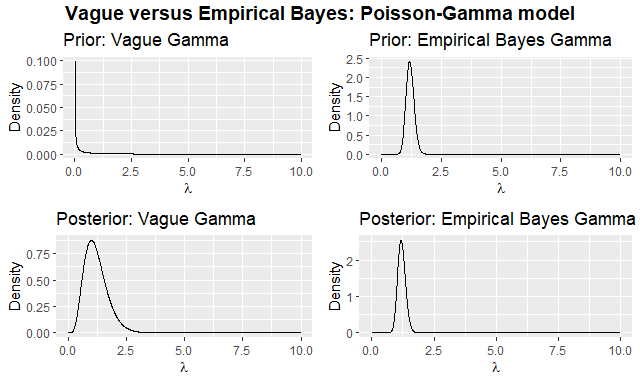
\includegraphics[width=340pt, height=200pt]{Chapters/chapter1/figures/PoisGam.png}
	%%\centerline{\epsfig{/Chapters/chapter1/figures/cat.eps,width=.8\textheight,height=.4\textwidth}}
	\caption[List of figure caption goes here]{Vague versus Empirical Bayes: Poisson-Gamma model.}\label{fig12}
\end{figure}

\begin{figure}[!h]
	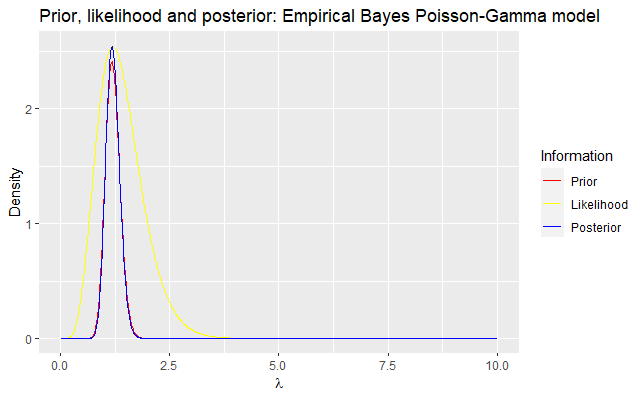
\includegraphics[width=340pt, height=200pt]{Chapters/chapter1/figures/PriorLikPost.png}
	%%\centerline{\epsfig{/Chapters/chapter1/figures/cat.eps,width=.8\textheight,height=.4\textwidth}}
	\caption[List of figure caption goes here]{Prior, likelihood and posterior: Empirical Bayes Poisson-Gamma model.}\label{fig13}
\end{figure}

Figure \ref{fig12} displays prior and posterior densities based on vague and Empirical Bayes hyperparameters. We see that prior and posterior densities using the latter are more informative as expected.

Figure \ref{fig13} shows the prior, scaled likelihood and posterior densities of $\lambda$ based on the hyperparameters of the Empirical Bayes approach. The posterior density is a compromise between prior and sample information. 

\clearpage
\begin{tcolorbox}[enhanced,width=4.67in,center upper,
	fontupper=\large\bfseries,drop shadow southwest,sharp corners]
\textit{R code. Health insurance, Predictive density}
\begin{VF}
\begin{lstlisting}[
	 language=R]
# Predictive distributions
PredDen <- function(y, y0, a0, b0){
	N <- length(y)
	#sample size
	an <- a0 + sum(y) 
	# Posterior shape parameter
	bn <- b0 / ((b0 * N) + 1) 
	# Posterior scale parameter
	p <- bn / (bn + 1) 
	# Probability negative binomial density
	Pr <- dnbinom(y0, size=an, prob=(1 - p))
	# Predictive density
	# Observe that in R there is a slightly different parametrization.
	return(Pr)
}
y0 <- 0:10
PredVague <- PredDen(y=y, y0=y0, a0=a0, b0=b0)
PredEB <- PredDen(y=y, y0=y0, a0=a0EB, b0=b0EB)
dataPred <- as.data.frame(cbind(y0, PredVague, PredEB))
colnames(dataPred) <- c("y0", "PredictiveVague", "PredictiveEB")
ggplot(data = dataPred) + geom_point(aes(y0, PredictiveVague, color = "red")) +  
xlab(TeX("$y_0$")) + ylab("Density") + ggtitle("Predictive density: Vague and Empirical Bayes priors") + geom_point(aes(y0, PredictiveEB, color = "yellow")) +
guides(color = guide_legend(title="Prior")) + scale_color_manual(labels = c("Vague", "Empirical Bayes"), values = c("red", "yellow")) + scale_x_continuous(breaks=seq(0,10,by=1))
\end{lstlisting}
\end{VF}
\end{tcolorbox}

\begin{figure}[!h]
	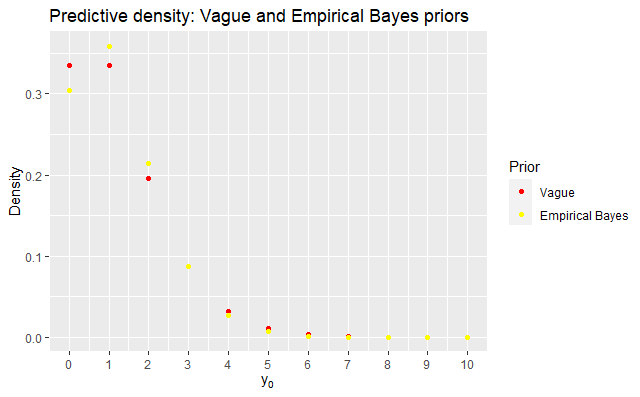
\includegraphics[width=340pt, height=200pt]{Chapters/chapter1/figures/Predictive.png}
	%%\centerline{\epsfig{/Chapters/chapter1/figures/cat.eps,width=.8\textheight,height=.4\textwidth}}
	\caption[List of figure caption goes here]{Predictive density: Vague and Empirical Bayes.}\label{fig14}
\end{figure}

Figure \ref{fig14} displays the predictive probability mass of not having any visits to a physician the next year, having one, two, and so on using Empirical Bayes and vague hyperparameters. The predictive probability of not having any visits are approximately equal to 30\% and 33\% based on the Empirical Bayes and vague hyperparameters. 

\begin{tcolorbox}[enhanced,width=4.67in,center upper,
	fontupper=\large\bfseries,drop shadow southwest,sharp corners]
\textit{R code. Health insurance, Bayesian model average}
\begin{VF}
\begin{lstlisting}[language=R]
# Posterior odds: Vague vs Empirical Bayes
PO12 <- exp(-LogMgLik(c(a0EB, b0EB), y = y))/exp(-LogMgLik(c(a0, b0), y = y))
PO12
919
PostProMEM <- PO12/(1 + PO12) 
PostProMEM
0.998
# Posterior model probability Empirical Bayes
PostProbMV <- 1 - PostProMEM 
PostProbMV
0.002
# Posterior model probability vague prior
# Bayesian model average (BMA)
PostMeanEB <- (a0EB + sum(y)) * (b0EB / (b0EB * N + 1)) 
# Posterior mean Empirical Bayes 
PostMeanV <- (a0 + sum(y)) * (b0 / (b0 * N + 1)) 
# Posterior mean vague priors
BMAmean <- PostProMEM * PostMeanEB + PostProbMV * PostMeanV  
BMAmean
1.2
# BMA posterior mean
PostVarEB <- (a0EB + sum(y)) * (b0EB/(b0EB * N + 1))^2 
# Posterior variance Empirical Bayes
PostVarV <- (a0 + sum(y)) * (b0 / (b0 * N + 1))^2 
# Posterior variance vague prior 
BMAVar <- PostProMEM * PostVarEB + PostProbMV*PostVarV + PostProMEM * (PostMeanEB - BMAmean)^2 + PostProbMV * (PostMeanV - BMAmean)^2
# BMA posterior variance   
BMAVar
0.025    
\end{lstlisting}
\end{VF}
\end{tcolorbox}

\begin{tcolorbox}[enhanced,width=4.67in,center upper,
	fontupper=\large\bfseries,drop shadow southwest,sharp corners]
	\textit{R code. Health insurance, Bayesian model average}
	\begin{VF}
		\begin{lstlisting}[ language=R]
# BMA: Predictive
BMAPred <- PostProMEM * PredEB+PostProbMV * PredVague
dataPredBMA <- as.data.frame(cbind(y0, BMAPred))
colnames(dataPredBMA) <- c("y0", "PredictiveBMA")
ggplot(data = dataPredBMA) + geom_point(aes(y0, PredictiveBMA, color = "red")) +  xlab(TeX("$y_0$")) + ylab("Density") + ggtitle("Predictive density: BMA") + guides(color = guide_legend(title="BMA")) + scale_color_manual(labels = c("Probability"), values = c("red")) + scale_x_continuous(breaks=seq(0,10,by=1)) 
		\end{lstlisting}
	\end{VF}
\end{tcolorbox}

\begin{figure}[!h]
	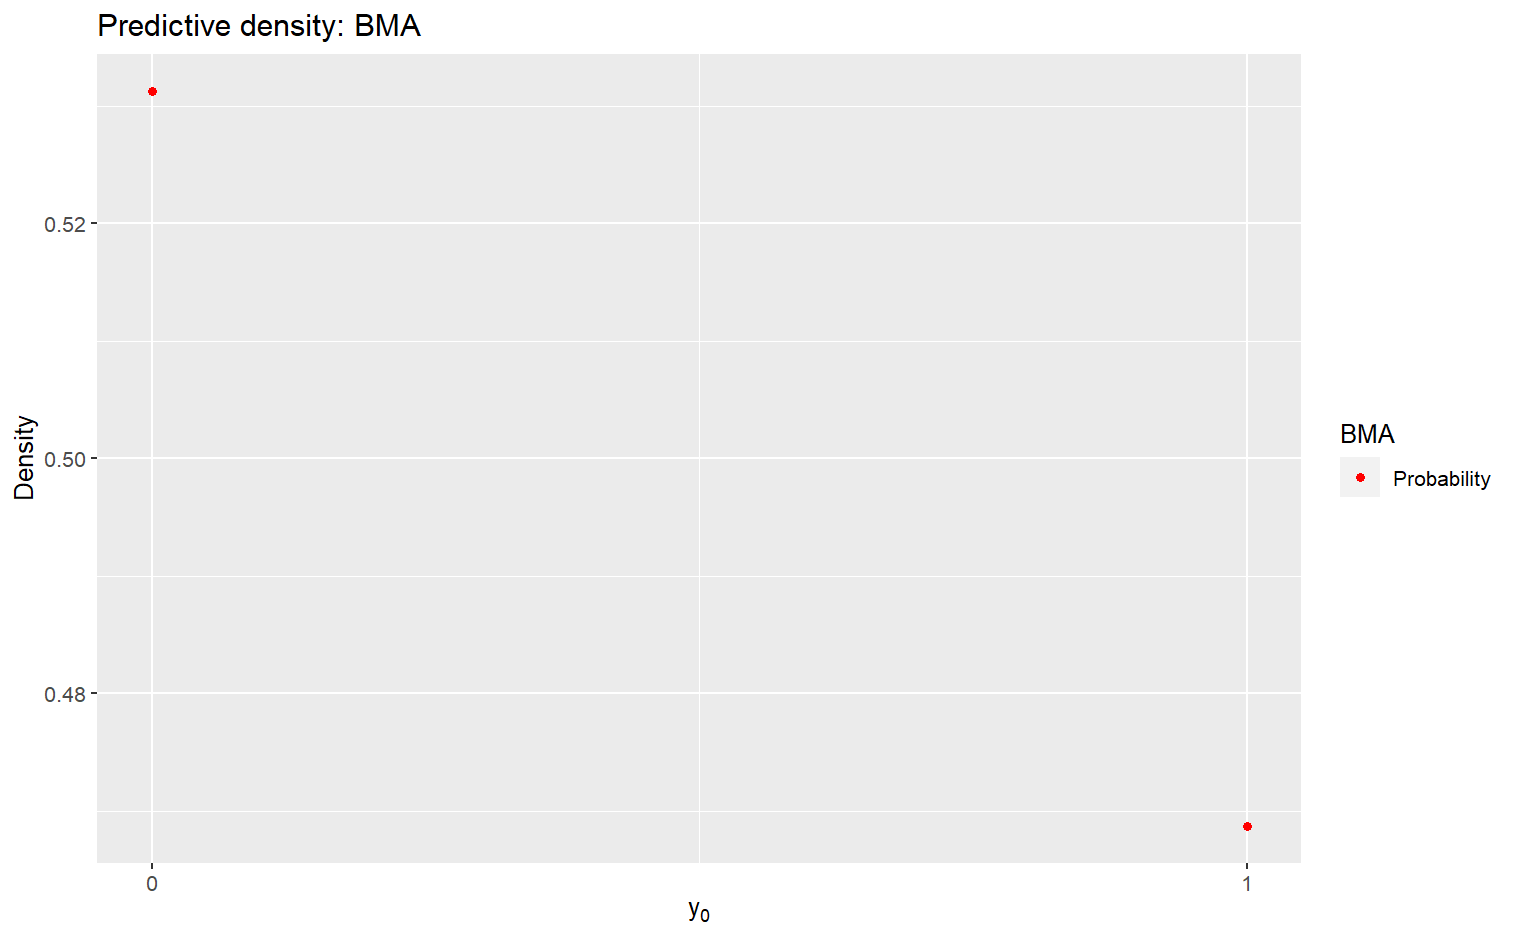
\includegraphics[width=340pt, height=200pt]{Chapters/chapter1/figures/BMA.png}
	%%\centerline{\epsfig{/Chapters/chapter1/figures/cat.eps,width=.8\textheight,height=.4\textwidth}}
	\caption[List of figure caption goes here]{Bayesian model average: Predictive density.}\label{fig15}
\end{figure}

\begin{figure}[!h]
	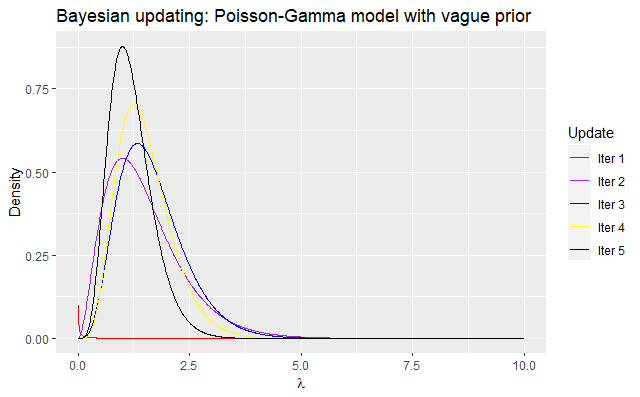
\includegraphics[width=340pt, height=200pt]{Chapters/chapter1/figures/Updating.png}
	%%\centerline{\epsfig{/Chapters/chapter1/figures/cat.eps,width=.8\textheight,height=.4\textwidth}}
	\caption[List of figure caption goes here]{Bayesian updating: Posterior densities.}\label{fig16}
\end{figure}

Figure \ref{fig15} displays the predictive density using Bayesian model average based on the vague and Empirical Bayes hyperparameters. This figure essentially resembles the predictive probability mass function based on the Empirical Bayes framework, as the posterior model probability for that setting is nearly one.

Figure \ref{fig16} displays how the posterior distribution updates given new sample information based on an initial non-informative prior (iteration 1). We see that iteration 5 is based on all the sample information in our example, as a consequence, the posterior density in iteration 5 is equal to the posterior density in Figure \ref{fig13}.

\begin{tcolorbox}[enhanced,width=4.67in,center upper,
	fontupper=\large\bfseries,drop shadow southwest,sharp corners]
\textit{R code. Health insurance, Bayes updating}
\begin{VF}
\begin{lstlisting}[ language=R]
# Bayesian updating
BayUp <- function(y, lambda, a0, b0){
	N <- length(y)
	#sample size
	an <- a0 + sum(y) 
	# Posterior shape parameter
	bn <- b0 / ((b0 * N) + 1) 
	# Posterior scale parameter
	p <- dgamma(lambda, shape = an, scale = bn) 
	# Posterior density
	return(list(Post = p, a0New = an, b0New = bn))
}
PostUp <- NULL
for(i in 1:N){
	if(i == 1){
		PostUpi <- BayUp(y[i], lambda, a0 = 0.001, b0 = 1/0.001)}
	else{
		PostUpi <- BayUp(y[i], lambda, a0 = PostUpi$a0New, b0 = PostUpi$b0New)
	}
	PostUp <- cbind(PostUp, PostUpi$Post)
}
DataUp <- data.frame(cbind(rep(lambda, 5), c(PostUp), rep(1:5, each = 1000))) #Data frame
colnames(DataUp) <- c("Lambda", "Density", "Factor")
DataUp$Factor <- factor(DataUp$Factor, levels=c("1", "2", "3", "4", "5"), 
labels=c("Iter 1", "Iter 2", "Iter 3", "Iter 4", "Iter 5"))
ggplot(data = DataUp, aes_string(x = "Lambda", y = "Density", group = "Factor")) + geom_line(aes(color = Factor)) + xlab(TeX("$\\lambda$")) + ylab("Density") + ggtitle("Bayesian updating: Poisson-Gamma model with vague prior") + guides(color=guide_legend(title="Update")) + scale_color_manual(values = c("red", "purple", "blue", "yellow", "black"))
S <- 100000 # Posterior draws
PostMeanLambdaUps <- sapply(1:N, function(i) {mean(sample(lambda, S, replace = TRUE, prob = PostUp[ , i]))}) #Posterior mean update i
paste("Posterior means using all information and sequential updating are:", round(PostMeanV, 2), "and", round(PostMeanLambdaUps[5], 2), sep = " ")
Posterior means using all information and sequential updating are: 1.2 and 1.2 
PostVarLambdaUps <- sapply(1:N, function(i) {var(sample(lambda, S, replace = TRUE, prob = PostUp[ , i]))}) #Posterior variance update i
paste("Posterior variances using all information and sequential updating are:", round(PostVarV, 2), "and", round(PostVarLambdaUps[5], 2), sep = " ")
Posterior variances using all information and sequential updating are: 0.24 and 0.24
\end{lstlisting}
\end{VF}
\end{tcolorbox}

\section{Bayesian reports: Decision theory under uncertainty}\label{sec14}

The Bayesian framework allows reporting the full posterior distributions. However, some situations demand to report a specific value of the posterior distribution (point estimate), an informative interval (set), point or interval predictions and/or selecting a specific model. Decision theory offers an elegant framework to make a decision regarding what are the optimal posterior values to report \cite{berger2013statistical}.

The point of departure is a \textit{loss function}, which is a non-negative real value function whose arguments are the unknown \textit{state of nature} ($\mathbf{\Theta}$), and a set of \textit{actions} to be made ($\mathcal{A}$), that is, 
\begin{equation*}
	L(\bm{\theta}, a):\mathbf{\Theta}\times \mathcal{A}\rightarrow \mathcal{R}^+.
\end{equation*}

This function is a mathematical expression of the loss of making mistakes. In particular, selecting action $a\in\mathcal{A}$ when $\bm{\theta}\in\mathbf{\Theta}$ is the true. In our case, the unknown state of nature can be parameters, functions of them, future or unknown realizations, models, etc.

From a Bayesian perspective, we should choose the action that minimizes the posterior expected loss ($a^*(\mathbf{y})$), that is, the \textit{posterior risk function} ($\mathbb{E}[L(\bm{\theta}, a)|\mathbf{y}]$),

\begin{equation*}
	a^*(\mathbf{y})=\underset{a \in \mathcal{A}}{\mathrm{argmin}} \  \mathbb{E}[L(\bm{\theta}, a)|\mathbf{y}], 
\end{equation*}

where $\mathbb{E}[L(\bm{\theta}, a)|\mathbf{y}]= \int_{\mathbf{\Theta}} L(\bm{\theta}, a)\pi(\bm{\theta}|\mathbf{y})d\bm{\theta}$.\footnote{\cite{Chernozhukov2003} propose Laplace type estimators (LTE) based on the \textit{quasi-posterior}, $p(\bm{\theta})=\frac{\exp\left\{L_n(\bm{\theta})\right\}\pi(\bm{\theta})}{\int_{\mathbf{\Theta}}\exp\left\{L_n(\bm{\theta})\right\}\pi(\bm{\theta})d\theta}$ where $L_n(\bm{\theta})$ is not necessarily a log-likelihood function. The LTE minimizes the \textit{quasi-posterior risk}.}

Different loss functions imply different optimal decisions. We illustrate this assuming $\theta \in \mathcal{R}$.

\begin{itemize}
	\item The quadratic loss function, $L({\theta},a)=[{\theta}-a]^2$, gives as optimal decision the posterior mean, $a^*(\mathbf{y})=\mathbb{E}[{\theta}|\mathbf{y}]$, that is 
		
	\begin{equation*}
		\mathbb{E}[{\theta}|\mathbf{y}] = \underset{a \in \mathcal{A}}{\mathrm{argmin}} \  \int_{{\Theta}} [{\theta}-a]^2\pi({\theta}|\mathbf{y})d{\theta}.
	\end{equation*}
	
	To get this results, let's use the first condition order, differentiate the risk function with respect to $a$, interchange differential and integral order, and set this equal to zero, $-2\int_{{\Theta}} [{\theta}-a^*]\pi({\theta}|\mathbf{y})d{\theta}=0$ implies that $a^*\int_{{\Theta}} \pi({\theta}|\mathbf{y})d{\theta}=a^*(\mathbf{y})=\int_{{\Theta}} {\theta}\pi({\theta}|\mathbf{y})d{\theta}=\mathbb{E}[{\theta}|\mathbf{y}]$, that is, the posterior mean is the Bayesian optimal action. This means that we should report the posterior mean as a point estimate of $\theta$ when facing the quadratic loss function.
	
	\item The generalized quadratic loss function,  $L({\theta},a)=w({\theta})[{\theta}-a]^2$, where $w({\theta})>0$ is a weighting function, gives as optimal decision rule the weighted mean. We should follow same steps as the previous result to get   $a^*(\mathbf{y})=\frac{\mathbb{E}[w({\theta})\times{\theta}|\mathbf{y}]}{\mathbb{E}[w({\theta})|\mathbf{y}]}$. Observe that the weighted average is driven by the weighting function $w({\theta})$.
	
	\item The absolute error loss function, $L({\theta},a)=|{\theta}-a|$, gives as optimal action the posterior median (Exercise 5).
	
	\item The generalized absolute error function,
	
	\begin{equation*}
		L(\theta,a)=\begin{Bmatrix} K_0(\theta-a), \theta-a\geq 0\\
			K_1(a-\theta), \theta-a < 0 \end{Bmatrix}, \ K_0,K_1>0,
	\end{equation*}
	
	implies the following risk function,
	
	\begin{align*}
		\mathbb{E}[L(\theta, a)|\mathbf{y}]&=\int_{-\infty}^a K_1(a-\theta)\pi(\theta|\mathbf{y})d\theta + \int_a^{\infty} K_0(\theta-a)\pi(\theta|\mathbf{y})d\theta. 
	\end{align*}
	
	Differentiating with respect to $a$, interchanging differentials and integrals, and equating to zero,
	\begin{align*}
		K_1\int_{-\infty}^{a^*} \pi(\theta|\mathbf{y})d\theta-K_0\int_{a^*}^{\infty} \pi(\theta|\mathbf{y})d\theta&=0,
	\end{align*}
	
	then, $\int_{-\infty}^{a^*} \pi(\theta|\mathbf{y})d\theta=\frac{K_0}{K_0+K_1}$, that is, any $K_0/(K_0+K_1)$-percentile of $\pi(\theta|\mathbf{y})$ is an optimal Bayesian estimate of $\theta$. 
\end{itemize}

We can also use decision theory under uncertainty in hypothesis testing. In particular, testing $H_0:\theta\in\Theta_0$ versus $H_1:\theta\in\Theta_1$, $\Theta=\Theta_0 \cup \Theta_1$ and $\emptyset=\Theta_0 \cap \Theta_1$, there are two actions of interest, $a_0$ and $a_1$, where $a_j$ denotes no rejecting $H_j$, $j=\left\{0,1\right\}$. 

Given the $0-K_j$ loss function,

\begin{equation*}
	L(\theta,a_j)=\begin{Bmatrix} 0, & \theta\in\Theta_j\\
		K_j, & \theta\in\Theta_j, j\neq i \end{Bmatrix},
\end{equation*}

where there is no loss if the right decision is made, for instance, no rejecting $H_0$ when $\theta\in\Theta_0$, and the loss is $K_j$ when an error is made, for instance, type I error, rejecting the null hypothesis ($H_0$) when it is true ($\theta\in\Theta_0$), implies a loss equal to $K_1$ due to picking $a_1$, no rejecting $H_1$. 

The posterior expected loss associated with decision $a_j$, that is, no rejecting $H_j$, is $\mathbb{E}[L(\theta,a_j)|\mathbf{y}]=0\times P(\Theta_j|\mathbf{y}) + K_jP(\Theta_i|\mathbf{y})=K_jP(\Theta_i|\mathbf{y})$, $j\neq i$. Therefore, the Bayes optimal decision is the one that gives the smallest posterior expected loss, that is, the null hypothesis is rejected ($a_1$ is not rejected), when $K_0P(\Theta_1|\mathbf{y}) > K_1P(\Theta_0|\mathbf{y})$. Given our framework $(\Theta=\Theta_0 \cup \Theta_1, \emptyset=\Theta_0 \cap \Theta_1)$, then $P(\Theta_0|\mathbf{y})=1-P(\Theta_1|\mathbf{y})$, and as a consequence, $P(\Theta_1|\mathbf{y})>\frac{K_1}{K_1+K_0}$, that is, the rejection region of the Bayesian test is $R=\left\{\mathbf{y}:P(\Theta_1|\mathbf{y})>\frac{K_1}{K_1+K_0}\right\}$.

Decision theory also helps to construct interval (region) estimates. Let $\Theta_{C(\mathbf{y})}\subset \Theta$ a \textit{credible set} for $\theta$, and $L(\theta,\Theta_{C(\mathbf{y})})=1-\mathbbm{1}\left\{\theta\in \Theta_{C(\mathbf{y})}\right\}$, where 

\begin{equation*}
	\mathbbm{1}\left\{\theta\in \Theta_{C(\mathbf{y})}\right\}=\begin{Bmatrix}1, & \theta\in \Theta_{C(\mathbf{y})}\\  
		0, & \theta\notin \Theta_{C(\mathbf{y})}
	\end{Bmatrix}.
\end{equation*}

Then,

\begin{equation*}
	L(\theta,\Theta_{C(\mathbf{y})})=\begin{Bmatrix}0, & \theta\in \Theta_{C(\mathbf{y})}\\  
		1, & \theta\notin \Theta_{C(\mathbf{y})}
	\end{Bmatrix},
\end{equation*}

where the 0--1 loss function is equal to zero if $\theta\in \Theta_{C(\mathbf{y})}$, and one if $\theta\notin \Theta_{C(\mathbf{y})}$. Then, the risk function is $1-P(\theta\in \Theta_{C(\mathbf{y})})$.

Given a \textit{measure of credibility} ($\alpha(\mathbf{y})$) that defines the level of trust that $\theta\in \Theta_{C(\mathbf{y})}$; then, we can measure the accuracy of the report by $L(\theta, \alpha(\mathbf{y}))=[\mathbbm{1}\left\{\theta\in \Theta_{C(\mathbf{y})}\right\}-\alpha(\mathbf{y})]^2$. This loss function could be used to suggest a choice of the report $\alpha(\mathbf{y})$. Given that this is a quadratic loss function, the optimal action is the posterior mean, that is $\mathbb{E}[\mathbbm{1}\left\{\theta\in \Theta_{C(\mathbf{y})}\right\}|\mathbf{y}]=P(\theta\in \Theta_{C(\mathbf{y})}|\mathbf{y})$. This probability can be calculated given the posterior distribution, that is, $P(\theta\in \Theta_{C(\mathbf{y})}|\mathbf{y})=\int_{\Theta_{C(\mathbf{y})}}\pi(\theta|\mathbf{y})d\theta$. This is a measure of the belief that $\theta\in \Theta_{C(\mathbf{y})}$ given the prior beliefs and sample information.

The set $\Theta_{C(\mathbf{y})}\in\Theta$ is a $100(1-\alpha)\%$ credible set with respect to $\pi(\theta|\mathbf{y})$ if $P(\theta\in \Theta_{C(\mathbf{y})}|\mathbf{y})=\int_{\Theta_{C(\mathbf{y})}}\pi(\theta|\mathbf{y})=1-\alpha$.

Two alternatives to report credible sets are the \textit{symmetric credible set} and the \textit{highest posterior density set} (HPD). The former is based on $\frac{\alpha}{2}$\% and $(1-\frac{\alpha}{2})$\% percentiles of the posterior distribution, and the latter is a $100(1-\alpha)\%$ credible interval for $\theta$ with the property that it has the smallest distance compared to any other $100(1-\alpha)\%$ credible interval for $\theta$ based on the posterior distribution. That is, $C(\mathbf{y})=\left\{\theta:\pi(\theta|\mathbf{y})\geq k(\alpha)\right\}$, where $k(\alpha)$ is the largest number such that $\int_{\theta:\pi(\theta|\mathbf{y})\geq k(\alpha)}\pi(\theta|\mathbf{y})d\theta=1-\alpha$. The HPD set can be a collection of disjoint intervals when working with multimodal posterior densities. In addition, they have the limitation of not necessary being invariant under transformations. 

Decision theory can also be used to perform prediction (point, sets or probabilistic). Suppose that there is a loss function $L(Y_0,a)$ involving the prediction of $Y_0$. Then, $\mathbb{E}_{Y_0}[L(Y_0,a)]=\int_{\mathcal{Y}_0}L(Y_0,a)\pi(Y_0|\mathbf{y})dY_0$, where $\pi(Y_0|\mathbf{y})$ is the predictive density function. Thus, we make an optimal choice for prediction that minimizes the risk function given a specific loss function.

Although BMA allows incorporating model uncertainty in a regression framework, sometimes it is desirable to select just one model. A compelling alternative is the model with the highest posterior model probability. This model is the best alternative for prediction in the case of a 0--1 loss function \cite{Clyde2004}.

\subsection{Example: Health insurance continues}\label{131}

We show some optimal rules in the health insurance example. In particular, the best point estimates of $\lambda$ given the quadratic, absolute and generalized absolute loss functions. For the third, we assume that underestimating $\lambda$ is twice as costly as overestimating it, that is, $K_0=2$ and $K_1=1$.

Taking into account that the posterior distribution of $\lambda$ is $G(\alpha_0+\sum_{i=1}^N y_i, \beta_0/(\beta_0N+1))$, using the hyperparameters from empirical Bayes, we have that $\mathbb{E}[\lambda|\mathbf{y}]=\alpha_n\beta_n=1.2$, the median is 1.19, and the 2/3-th quantile is 1.26. Those are the optimal point estimates for the quadratic, absolute and generalized absolute loss functions.

In addition, we test the null hypothesis $H_0. \ \lambda \in [0,1)$ versus $H_1. \ \lambda \in [1,\infty)$ setting $K_0=K_1=1$ we should reject the null hypothesis due to $P(\lambda \in [0,1))=0.9>K_1/(K_0+K_1)=0.5$.

We get that the 95\% symmetric credible interval is (0.91, 1.53), and the highest posterior density interval is (0.9, 1.51). Finally, the optimal point prediction under a quadratic loss function is 1.2, which is the mean value of the posterior predictive distribution, and the optimal model assuming a 0-1 loss function is the model using the hyperparameters from the empirical Bayes procedure due to the posterior model probability of this model being approximately 1, whereas the posterior model probability of the model using vague hyperparameters is approximately 0.

\begin{tcolorbox}[enhanced,width=4.67in,center upper,
	fontupper=\large\bfseries,drop shadow southwest,sharp corners]
	\textit{R code. Health insurance, Bayesian reports}
\begin{VF}
\begin{lstlisting}[ language=R]
an <- sum(y) + a0EB 
# Posterior shape parameter
bn <- b0EB / (N*b0EB + 1) 
# Posterior scale parameter
S <- 1000000 
# Number of posterior draws
Draws <- rgamma(1000000, shape = an, scale = bn) 
# Posterior draws
###### Point estimation ########
OptQua <- an*bn 
# Mean: Optimal choice quadratic loss function
OptQua
1.200952
OptAbs <- qgamma(0.5, shape = an, scale = bn) 
# Median: Optimal choice absolute loss function
OptAbs
1.194034
# Setting K0 = 2 and K1 = 1, that is, to underestimate lambda is twice as costly as to overestimate it.
K0 <- 2; K1 <- 1
OptGenAbs <- quantile(Draws, K0/(K0 + K1)) 
# Median: Optimal choice generalized absolute loss function
OptGenAbs
66.66667% 
1.262986 
###### Hypothesis test ########
# H0: lambda in [0,1) vs H1: lambda in [1, Inf]
K0 <- 1; K1 <- 1
ProbH0 <- pgamma(1, shape = an, scale = bn) 
ProbH0 # Posterior  probability H0
0.09569011
ProbH1 <- 1 -ProbH0
ProbH1 # Posterior  probability H1
0.9043099
# We should reject H0 given ProbH1 > K1 / (K0 + K1) 
###### Credible intervals ########
LimInf <- qgamma(0.025, shape = an, scale = bn) # Lower bound
LimInf
0.9114851
LimSup <- qgamma(0.975, shape = an, scale = bn) # Upper bound
LimSup
1.529724
HDI <- HDInterval::hdi(Draws, credMass = 0.95) # Highest posterior density credible interval
HDI
    lower     upper 
0.8971505 1.5125911 
attr(,"credMass")
[1] 0.95
###### Predictive optimal choices ########
p <- bn / (bn + 1) # Probability negative binomial density
OptPred <- p/(1-p)*an # Optimal point prediction given a quadratic loss function in prediction
OptPred
1.200952
\end{lstlisting}
\end{VF}
\end{tcolorbox}

\section{Summary}
We introduce the Bayes' rule to update probabilistic statements using funny examples. Then, we study  the three probabilistic objects of main relevance in Bayesian inference: the posterior distribution, the marginal likelihood and the predictive density. The first allows performing inference regarding parameters, the second is required to perform hypothesis test for model selection using the Bayes factor, and the third to perform probabilistic predictions. We also review some sampling properties of Bayesian estimators, and Bayes update. All those concepts were developed using a simple example in R software. Finally, we introduce some concepts of decision theory that can be used to report summary statistics minimizing posterior expected losses.
 
\section{Exercises}

\begin{enumerate}
	\item \textit{The court case: the blue or green cap}
	
	A cab was involved in a hit and run accident at night. There are two cab companies in the town: blue and green. The former has 150 cabs, and the latter 850 cabs. A witness said that a blue cab was involved in the accident; the court tested his/her reliability under the same circumstances, and got that 80\% of the times the witness correctly identified the color of the cab. \textit{What is the probability that the color of the cab involved in the accident was blue given that the witness said it was blue?}
	
	\item \textit{The Monty Hall problem}
	
	What is the probability of winning a car in the \textit{Monty Hall problem} switching the decision if there are four doors, where there are three goats and one car? Solve this problem analytically and computationally.  What if there are $n$ doors, $n-1$ goats and one car?
	
	\item Solve the health insurance example using a Gamma prior in the rate parametrization, that is, $\pi(\lambda)=\frac{\beta_0^{\alpha_0}}{\Gamma(\alpha_0)}\lambda^{\alpha_0-1}\exp\left\{-\lambda\beta_0\right\}$.  
	
	\item Suppose that you are analyzing to buy a car insurance next year. To make a better decision you want to know \textit{what is the probability that you have a car claim next year?} You have the records of your car claims in the last 15 years, $\mathbf{y}=\left\{0, 1, 0, 1, 0, 1, 1, 0, 0, 1, 0, 0, 1, 1, 0\right\}$.
	
	Assume that this is a random sample from a data generating process (statistical model) that is Bernoulli, $Y_i\sim Ber(p)$, and your probabilistic prior beliefs about $p$ are well described by a beta distribution with parameters $\alpha_0$ and $\beta_0$, $p\sim B(\alpha_0, \beta_0)$, then, you are interested in calculating the probability of a claim the next year $P(Y_0 = 1|\mathbf{y})$.
	
	Solve this using an empirical Bayes approach and a non-informative approach where $\alpha_0=\beta_0=1$ (uniform distribution). 
	
	\item Show that given the loss function, $L({\theta},a)=|{\theta}-a|$, then the optimal decision rule minimizing the risk function, $a^*(\mathbf{y})$, is the median.

\end{enumerate}




\chapter{Conceptual differences of the Bayesian and Frequentist approaches}\label{chap2}
\section{Solutions of Exercises}\label{sec21}
\begin{enumerate}[leftmargin=*]
\item \textbf{Jeffreys-Lindley's paradox}

The \textbf{Jeffreys-Lindley's paradox} \cite{Jeffreys1961,lindley1957statistical} is an apparent disagreement between the Bayesian and Frequentist frameworks to a hypothesis testing situation.

In particular, assume that in a city 49,581 boys and 48,870 girls have been born in 20 years. Assume that the male births is distributed Binomial with probability $\theta$. We want to test the null hypothesis $H_0. \ \theta=0.5$ versus $H_1. \ \theta\neq 0.5$.

\begin{itemize}
	\item Show that the posterior model probability for the model under the null is approximately 0.95. Assume $\pi(H_0)=\pi(H_1)=0.5$, and $\pi(\theta)$ equal to ${U}(0,1)$ under $H_1$.
	\item Show that the \textit{p}-value for this hypothesis test is equal to 0.023 using the normal approximation, $Y\sim {N}(N\times \theta, N\times \theta \times (1-\theta))$. 
\end{itemize}

\textbf{Answer}

\begin{itemize}
	\item The marginal likelihood under the null hypothesis is $p(y|H_0)={n \choose y}\theta^y(1-\theta)^{n-y}\approx 1.95\times 10^{-4}$ given $\theta=0.5$ under $H_0$, $N=49,581+48,870$ and $y=49,581$. On the other hand, the marginal likelihood under the alternative hypothesis is

\begin{align*}
	p(y|H_1)&=\int_{0}^{1}{n \choose y}\theta^y(1-\theta)^{n-y}d\theta\\
	&={n \choose y} B(y+1, n-k+1)\\
	&=\frac{\Gamma(N+1)}{\Gamma(y+1)\Gamma(n-y+1)}\frac{\Gamma(y+1)\Gamma(N-y+1)}{\Gamma(N+2)}\\
	&=\frac{N!}{(N+1)!}\\
	&=\frac{1}{N+1}\\
	&\approx1.016\times 10^{-5}. 
\end{align*}

Then, $PO_{01}=\frac{1.95\times 10^{-4}}{1.016\times 10^{-5}}=19.19$, this implies that the posterior model probability under the null hypothesis is $\pi(H_0|y)=\frac{19.19}{1+19.19}=0.95$.

\item Under the null hypothesis, 

\begin{align*}
	p & = 2\int_{49,581}^{\infty} (2\pi \sigma^2)^{-1/2}\exp\left\{-\frac{1}{2\sigma^2}(y-\mu)^2\right\}dy\\
	& = 0.0235,
\end{align*}
 
 where $\mu=N\times \theta=49,225.5$, and $\sigma^{2}= N\times \theta \times (1-\theta)=24,612.75$ under the null hypothesis ($\theta = 0.5$).

\end{itemize}

Observe that the posterior model probability supports the null hypothesis, whereas the p-value implies rejection of the null hypothesis using a 5\% significance level.

Observe that actually this is not a paradox, as we are answering two different questions. The Bayes factor is comparing two models ($\theta = 0.5$ versus $\theta\sim{U}(0,1)$), whereas the \textit{p}-value is checking the compatibility between $\theta=0.5$ and the sample information. Despite that $\theta=0.5$ is not compatible with sample information, it is better than the models assuming $\theta\sim{U}(0,1)$ as most of these values of $\theta$ are far away from the sample mean. Thus, the model under the null is a bad description of the data, but it is better than the model under the alternative hypothesis.\footnote{Observe that there are at least another two issues in this example. First, the prior under the alternative is non-informative, this implies problems for Bayes factors, and second, the prior under the alternative is positive at $\theta=0.5$, which is the null (\cite{johnson2010use} propose non-local prior densities in Bayesian hypothesis tests to tackle these issues).}      

\item We want to test $H_0. \ \mu=\mu_0$ vs $H_1. \ \mu \neq \mu_0$ given $y_i\stackrel{iid}{\sim}N(\mu,\sigma^2)$.

Assume $\pi(H_0)=\pi(H_1)=0.5$, and $\pi(\mu,\sigma)\propto 1/\sigma$ under the alternative hypothesis.

Show that

$p(\mathbf{y}|\mathcal{M}_1)=\frac{\pi^{-N/2}}{2}\Gamma(N/2)2^{N/2}\left(\frac{1}{\alpha_n\hat{\sigma}^2}\right)^{N/2}\left(\frac{N}{\alpha_n\hat{\sigma}^2}\right)^{-1/2}\frac{\Gamma(1/2)\Gamma(\alpha_n/2)}{\Gamma((\alpha_N+1)/2)}$ and $p(\mathbf{y}|\mathcal{M}_0)=(2\pi)^{-N/2}\left[\frac{2}{\Gamma(N/2)}\left(\frac{N}{2}\frac{\sum_{i=1}^N(y_i-\mu_0)^2}{N}\right)^{N/2}\right]^{-1}$. Then,

\begin{align*}
	PO_{01}&=\frac{p(\mathbf{y}|\mathcal{M}_0)}{p(\mathbf{y}|\mathcal{M}_1)}\\
	& =\frac{\Gamma((\alpha_n+1)/2)}{\Gamma(1/2)\Gamma(\alpha_N/2)}(\alpha_n\hat{\sigma}^2/N)^{-1/2}\left[1+\frac{(\mu_0-\bar{y})^2}{\alpha_n\hat{\sigma}^2/N}\right]^{-\left(\frac{\alpha_n+1}{2}\right)},
\end{align*}

where $\alpha_N=N-1$ and $\hat{\sigma}^2=\frac{\sum_{i=1}^N (y_i-\bar{y})^2}{N-1}$. 

Find the relationship between the posterior odds and the classical test statistic for the null hypothesis. 

\textbf{Answer}
{\footnotesize{
\begin{align*}
	p(\mathbf{y}|\mathcal{M}_1)&=\int_{-\infty}^{\infty}\int_{0}^{\infty} (2\pi)^{-N/2}\sigma^{-N}\exp\left\{-\frac{1}{2\sigma^2}\sum_{i=1}^N (y_i-\mu)^2\right\}\frac{1}{\sigma}d\sigma d\mu\\
	&=(2\pi)^{-N/2}\int_{-\infty}^{\infty}\int_{0}^{\infty} \sigma^{-(N+1)}\exp\left\{-\frac{N}{2\sigma^2}\frac{\sum_{i=1}^N (y_i-\mu)^2}{N}\right\}d\sigma d\mu\\
	&=(2\pi)^{-N/2}\frac{\Gamma(N/2)}{2}2^{N/2}\int_{-\infty}^{\infty}\left[\sum_{i=1}^N (y_i-\mu)^2\right]^{-N/2}d\mu\\
	&=(2\pi)^{-N/2}\frac{\Gamma(N/2)}{2}2^{N/2}\int_{-\infty}^{\infty}\left[\sum_{i=1}^N [(y_i-\bar{y})-(\mu-\bar{y})]^2\right]^{-N/2}d\mu\\
	&=(2\pi)^{-N/2}\frac{\Gamma(N/2)}{2}2^{N/2}\int_{-\infty}^{\infty}\left[\alpha_n\hat{\sigma}^2+N(\mu-\bar{y})^2\right]^{-N/2}d\mu\\
	&=(2\pi)^{-N/2}\frac{\Gamma(N/2)}{2}2^{N/2}\left(\frac{\alpha_n\hat{\sigma}^2}{\alpha_n\hat{\sigma}^2}\right)^{-N/2}\int_{-\infty}^{\infty}\left[\alpha_n\hat{\sigma}^2+N(\mu-\bar{y})^2\right]^{-N/2}d\mu\\
	&=(2\pi)^{-N/2}\frac{\Gamma(N/2)}{2}2^{N/2}\left(\alpha_n\hat{\sigma}^2\right)^{-N/2}\int_{-\infty}^{\infty}\left[1+\frac{N(\mu-\bar{y})^2}{\alpha_n\hat{\sigma}^2}\right]^{-N/2}d\mu\\
	&=\frac{\pi^{-N/2}}{2}\Gamma(N/2)2^{N/2}\left(\frac{1}{\alpha_n\hat{\sigma}^2}\right)^{N/2}\left(\frac{N}{\alpha_n\hat{\sigma}^2}\right)^{-1/2}\frac{\Gamma(1/2)\Gamma(\alpha_n/2)}{\Gamma((\alpha_N+1)/2)}.
\end{align*} 
}}
The third line takes into account that the integral in the second line is the kernel of an inverted-gamma distribution, and the last line takes into account that the integral in the previous line is the kernel of a student's t distribution \cite{zellner1996introduction}.


\begin{align*}
	p(\mathbf{y}|\mathcal{M}_0)&=\int_{0}^{\infty} (2\pi)^{-N/2}\sigma^{-N}\exp\left\{-\frac{1}{2\sigma^2}\sum_{i=1}^N (y_i-\mu_0)^2\right\}\frac{1}{\sigma}d\sigma \\
	&=(2\pi)^{-N/2}\int_{0}^{\infty} \sigma^{-(N+1)}\exp\left\{-\frac{N}{2\sigma^2}\frac{\sum_{i=1}^N (y_i-\mu_0)^2}{N}\right\}d\sigma \\
	&=(2\pi)^{-N/2}\left[\frac{2}{\Gamma(N/2)}\left(\frac{N}{2}\frac{\sum_{i=1}^N(y_i-\mu_0)^2}{N}\right)^{N/2}\right]^{-1}.
\end{align*} 

The third line takes into account that the integral in the second line is the kernel of an inverted-gamma distribution \cite{zellner1996introduction}.

Given these results is easy to get $PO_{01}$.

In addition, 
\begin{align*}
	PO_{01}&=\frac{\Gamma((\alpha_n+1)/2)}{\Gamma(1/2)\Gamma(\alpha_N/2)}(\alpha_n\hat{\sigma}^2/N)^{-1/2}\left[1+\frac{(\mu_0-\bar{y})^2}{\alpha_n\hat{\sigma}^2/N}\right]^{-\left(\frac{\alpha_n+1}{2}\right)}\\
	&=\frac{\Gamma((\alpha_n+1)/2)}{\Gamma(1/2)\Gamma(\alpha_N/2)}(\alpha_n\hat{\sigma}^2/N)^{-1/2}\left[1+\frac{1}{\alpha_n}\left(\frac{\mu_0-\bar{y}}{\hat{\sigma}/\sqrt{N}}\right)^2\right]^{-\left(\frac{\alpha_n+1}{2}\right)}\\
		&=\frac{\Gamma((\alpha_n+1)/2)}{\Gamma(1/2)\Gamma(\alpha_N/2)}(\alpha_n\hat{\sigma}^2/N)^{-1/2}\left[1+\frac{1}{\alpha_n}t^2\right]^{-\left(\frac{\alpha_n+1}{2}\right)},	
\end{align*}

where $t=\frac{\bar{y}-\mu_0}{\hat{\sigma}/\sqrt{N}}$ is the classical statistical test. Then, as $t$ increases then the $PO_{01}$ decreases, both indicating support against the null hypothesis $H_0. \ \mu=\mu_0$. However, there are other terms affecting the posterior odds, then, there is no necessary agreement between the classical test statistic and the posterior odds.  

\item \textbf{Math test continues}

Using the setting of the \textbf{Example: Math test} in subsection 2.6.1 in the book, test $H_0. \ \mu=\mu_0$ vs $H_1. \ \mu \neq \mu_0$ where $\mu_0=\left\{100, 100.5, 101, 101.5, 102 \right\}$.

\begin{itemize}
	\item What is the \textit{p}-value for these hypothesis tests?
	\item Find the posterior model probability of the null model for each $\mu_0$.
\end{itemize} 

	\textbf{Answer}

\begin{tcolorbox}[enhanced,width=4.67in,center upper,
	fontupper=\large\bfseries,drop shadow southwest,sharp corners]
	\textit{R code. Example: Math test}
\begin{VF}
\begin{lstlisting}[language=R]
N <- 50 # Sample size
y_bar <- 102 # Sample mean 
s2 <- 10 # Sample variance
alpha <- N - 1
serror <- (s2/N)^0.5 
y.H0 <- c(100, 100.5, 101, 101.5, 102)
test <- (y.H0 - y_bar)/serror
pval <- 2*pt(test, alpha)
pval
0.0000459 0.0015431 0.0299338 0.2690040 1
# p-values
PO01 <- (gamma(N/2)*((N-1)*serror^2)^(-0.5)*(1+test^2/alpha)^(-N/2))/(gamma(1/2)*gamma((N-1)/2))
PO01/(1+PO01)
0.0001705 0.0050345 0.0725330 0.3210223 0.4702050
# Posterior model probability of the null hypothesis.
\end{lstlisting}
\end{VF}
\end{tcolorbox}

	
\end{enumerate}
\chapter{Cornerstone models: Conjugate families}\label{chap4}

\section{Solutions of Exercises}\label{sec1}
\begin{enumerate}[leftmargin=*]
\item Write in the canonical form the distribution of the Bernoulli example, and find the mean and variance of the sufficient statistic.

\textbf{Answer}

Given $p({\bf{y}}|\theta)=(1-\theta)^N\exp\left\{\sum_{i=1}^N y_i\log\left(\frac{\theta}{1-\theta}\right)\right\}$ where $\eta=\log\frac{\theta}{1+\theta}$ which implies $\theta=\frac{\exp(\eta)}{1-\exp(\eta)}$, then $p({\bf{y}}|\theta)=\exp\left\{\sum_{i=1}^N y_i\eta-N\log(1+\exp(\eta))\right\}$. Thus $B(\eta)=N\log(1+\exp(\eta))$, $\nabla(B(\eta))=N\frac{\exp(\eta)}{1+\exp(\eta)}=N\theta$ and $\nabla^2(B(\eta))=N\left\{\frac{\exp(\eta)(1+\exp(\eta))}{(1+\exp(\eta))^2}-\frac{\exp(\eta)\exp(\eta)}{(1+\exp(\eta))^2}\right\}=N\theta(1-\theta)$. 



\item Given a random sample $\mathbf{y}=[y_1,y_2,\dots,y_N]^{\top}$ from $N$ \textit{binomial experiments} each having known size $n_i$ and same unknown probability $\theta$. Show that $p(\mathbf{y}|\theta)$ is in the exponential family, and find the posterior distribution, the marginal likelihood and the predictive distribution of the binomial-beta model assuming the number of trials is known.

\textbf{Answer}

The density function is 
\begin{align*}
p({\bf{y}}|\theta)&=\prod_{i=1}^N{n_i \choose y_i}\theta^{y_i}(1-\theta)^{n_i-y_i}\\
&=\prod_{i=1}^N{n_i \choose y_i}\theta^{\sum_{i=1}^Ny_i}(1-\theta)^{\sum_{i=1}^N n_i-\sum_{i=1}^N y_i}\\
&=\prod_{i=1}^N{n_i \choose y_i}\exp\left\{\sum_{i=1}^N y_i\log\left(\frac{\theta}{1-\theta}\right)+\sum_{i=1}^N n_i\log(1-\theta)\right\}\\
&=\prod_{i=1}^N{n_i \choose y_i}(1-\theta)^{\sum_{i=1}^N n_i}\exp\left\{\sum_{i=1}^N y_i\log\left(\frac{\theta}{1-\theta}\right)\right\},
\end{align*}
 
Observe that $\sum_{i=1}^N n_i$ is the total sample size of Bernoulli experiments. 

Using Theorem 1 in Chapter 4, the prior distribution is \begin{align*}\pi(\theta)&\propto(1-\theta)^{B_0}\exp\left\{a_0\log\left(\frac{\theta}{1-\theta}\right)\right\}\\
	&=\theta^{a_0}(1-\theta)^{B_0-a_0}\\
	&=\theta^{\alpha_0-1}(1-\theta)^{\beta_0-1},
\end{align*}

where $\alpha_0=a_0+1$ and $\beta_0=B_0-a_0+1$. This is the kernel of a beta distribution. Thus, the posterior distribution is

\begin{align*}
	\pi(\theta|{\bf{y}})&\propto \theta^{\alpha_0-1}(1-\theta)^{\beta_0-1} \times \theta^{\sum_{i=1}^Ny_i}(1-\theta)^{\sum_{i=1}^N n_i-\sum_{i=1}^N y_i}\\
	&=\theta^{\alpha_0+\sum_{i=1}^Ny_i - 1}(1-\theta)^{\beta_0 + \sum_{i=1}^N n_i-\sum_{i=1}^N y_i - 1}\\
	&=\theta^{\alpha_n-1}(1-\theta)^{\beta_n-1},  
\end{align*}

where $\alpha_n = \alpha_0+\sum_{i=1}^Ny_i$ and $\beta_n=\beta_0 + \sum_{i=1}^N n_i-\sum_{i=1}^N y_i$.

The marginal likelihood is

\begin{align*}
	p({\bf{y}})&=\int_0^1 \frac{\theta^{\alpha_0-1}(1-\theta)^{\beta_0-1}}{B(\alpha_0,\beta_0)}\times \prod_{i=1}^N{n_i \choose y_i}\theta^{\sum_{i=1}^Ny_i}(1-\theta)^{\sum_{i=1}^N n_i-\sum_{i=1}^N y_i} d\theta\\
	&=\frac{ \prod_{i=1}^N{n_i \choose y_i}}{B(\alpha_0,\beta_0)}\int_0^1 \theta^{\alpha_0+\sum_{i=1}^Ny_i-1}(1-\theta)^{}\beta_0\sum_{i=1}^N n_i-\sum_{i=1}^N y_i-1 d\theta\\
	&=\frac{ \prod_{i=1}^N{n_i \choose y_i}B(\alpha_n,\beta_n)}{B(\alpha_0,\beta_0)}. 
\end{align*}

The third line due to having the kernel of a Beta distribution.

Finally, the predictive distribution is

\begin{align*}
	p(Y_0|{\bf{y}})&=\int_0^1 {n_{y_0} \choose y_0} \theta^{y_0}(1-\theta)^{n_{y_0}-y_0}\frac{\theta^{\alpha_n-1}(1-\theta)^{\beta_n-1}}{B(\alpha_n,\beta_n)}d\theta\\
	&=\frac{{n_{y_0} \choose y_0}}{B(\alpha_n,\beta_n)}\int_0^1  \theta^{\alpha_n+y_0-1}(1-\theta)^{\beta_n+n_{y_0}-y_0-1}d\theta\\
	&={n_{y_0} \choose y_0}\frac{B(\alpha_n+y_0,\beta_n+n_{y_0}-y_0)}{B(\alpha_n,\beta_n)},
\end{align*}

where $n_{y_0}$ is the known size associated with $y_0$, and the last line due to having the kernel of a beta distribution. The predictive is a \textit{beta-binomial distribution}.

\item Given a random sample $\mathbf{y}=[y_1,y_2,\dots,y_N]^{\top}$ from a \textit{exponential distribution}. Show that $p(\mathbf{y}|\lambda)$ is in the exponential family, and find the posterior distribution, marginal likelihood and predictive distribution of the exponential-gamma model.

\textbf{Answer}

We see that the exponential distribution belongs to the exponential family as $p({\bf{y}}|\lambda)=\prod_{i=1}^N\lambda\exp(-\lambda y_i)=\lambda^N\exp(-\lambda\sum_{i=1}^N y_i)$.

Using the gamma distribution in the rate parametrization, we see that $\pi(\lambda|{\bf{y}})\propto \lambda^{\alpha_0-1}\exp(-\lambda\beta_0)\times \lambda^N\exp(-\lambda\sum_{i=1}^N y_i)=\lambda^{\alpha_0+N-1}\exp(-\lambda(\beta_0+\sum_{i=1}^N y_i))$. This is the kernel of a gamma distribution, that is, $\lambda|{\bf{y}}\sim G(\alpha_n,\beta_n)$ where $\alpha_n=\alpha_0+N$ and $\beta_n=\beta_0+\sum_{i=1}^N y_i$.

The marginal likelihood is

\begin{align*}
	p({\bf{y}})&=\int_0^{\infty}\lambda^N \exp\left\{-\lambda\sum_{i=1}^N\right\}\lambda^{\alpha_0-1}\exp\left\{-\beta_0\lambda\right\}\frac{\beta_0^{\alpha_0}}{\Gamma(\alpha_0)}d\lambda\\
	&=\frac{\beta_0^{\alpha_0}}{\Gamma(\alpha_0)}\int_0^{\infty}\lambda^{\alpha_0+N-1} \exp\left\{-\lambda\left(\beta_0+\sum_{i=1}^N\right)\right\}d\lambda\\
	&=\frac{\beta_0^{\alpha_0}\Gamma(\alpha_n)}{\Gamma(\alpha_0)\beta_n^{\alpha_n}}.
\end{align*} 

Finally, the predictive distribution is

\begin{align*}
	p(Y_0|{\bf{y}})&=\int_0^{\infty}\lambda \exp\left\{-\lambda y_0\right\}\lambda^{\alpha_n-1}\exp\left\{-\beta_n\lambda\right\}\frac{\beta_n^{\alpha_n}}{\Gamma(\alpha_n)}d\lambda\\
	&=\frac{\beta_n^{\alpha_n}}{\Gamma(\alpha_n)}\int_0^{\infty}\lambda^{\alpha_n+1-1}\exp\left\{-\lambda(\beta_n+y_0)\right\}d\lambda\\
	&=\frac{\beta_n^{\alpha_n}}{\Gamma(\alpha_n)}\times \frac{\Gamma(\alpha_n+1)}{(\beta_n+y_0)^{\alpha_n+1}}\\
	&=\frac{\alpha_n\beta_n^{\alpha_n}}{(\beta_n+y_0)^{\alpha_n+1}}.
\end{align*} 

This is a \textit{Lomax distribution}.

\item Given $\mathbf{y}\sim N_N(\bm{\mu},\bm{\Sigma})$, that is, a \textit{multivariate normal distribution} show that $p(\mathbf{y}|\bm{\mu},\bm{\Sigma})$ is in the exponential family.

\textbf{Answer} 

\begin{align}
	p(\mathbf{y}|\bm{\mu},\bm{\Sigma})&= (2\pi)^{-N/2}|\bm{\Sigma}|^{-1/2}\exp\left\{-\frac{1}{2}\left(\mathbf{y}-\bm{\mu}\right)^{\top}\bm{\Sigma}^{-1}\left(\mathbf{y}-\bm{\mu}\right)\right\}\nonumber\\
	&= (2\pi)^{-N/2}\exp\left\{-\frac{1}{2}\left(\mathbf{y}^{\top}\bm{\Sigma}^{-1}\mathbf{y}-2\mathbf{y}^{\top}\bm{\Sigma}^{-1}\bm{\mu}+\bm{\mu}^{\top}\bm{\Sigma}^{-1}\bm{\mu}+\log(|\mathbf{\Sigma}|)\right)\right\}\nonumber\\
	&= (2\pi)^{-N/2}\exp\left\{-\frac{1}{2}\left(tr\left\{\mathbf{y}^{\top}\bm{\Sigma}^{-1}\mathbf{y}\right\}-2\mathbf{y}^{\top}\bm{\Sigma}^{-1}\bm{\mu}+\bm{\mu}^{\top}\bm{\Sigma}^{-1}\bm{\mu}+\log(|\mathbf{\Sigma}|)\right)\right\}\nonumber\\
	&= (2\pi)^{-N/2}\exp\left\{-\frac{1}{2}\left(vec\left(\mathbf{y}\mathbf{y}^{\top}\right)^{\top}vec\left(\bm{\Sigma}^{-1}\right)-2\mathbf{y}^{\top}\bm{\Sigma}^{-1}\bm{\mu}+\bm{\mu}^{\top}\bm{\Sigma}^{-1}\bm{\mu}+\log(|\mathbf{\Sigma}|)\right)\right\} \nonumber, 	
\end{align}

where $tr$ and $vec$ are the trace and vectorization operators, respectively. 

Then, $h(\mathbf{y})=(2\pi)^{-N/2}$, $\eta(\bm{\mu},\bm{\Sigma})=\left[\bm{\Sigma}^{-1}\bm{\mu} \ \ vec\left(\bm{\Sigma}^{-1}\right)\right]$, $T(\mathbf{y})=\left[\mathbf{y} \ \ -\frac{1}{2}vec(\mathbf{y}\mathbf{y}^{\top})\right]$ and $C(\bm{\mu},\bm{\Sigma})=\exp\left\{-\frac{1}{2N}\left(\bm{\mu}^{\top}\bm{\Sigma}^{-1}\bm{\mu}+\log(|\mathbf{\Sigma}|)\right)\right\}$.
	
\item Find the marginal likelihood in the normal/inverse-Wishart model.

\textbf{Answer}

\begin{align*}
	p({\bf{Y}})=&\int_{\mathcal{R}^p}\int_{\mathcal{S}}(2\pi)^{-pN/2}|\mathbf{\Sigma}|^{-N/2}\exp\left\{-\frac{1}{2}tr[({\bf{S}}+N(\bm{\mu}-\hat{\bm{\mu}})(\bm{\mu}-\hat{\bm{\mu}})^{\top})\mathbf{\Sigma}^{-1}]\right\}\\
	&\times (2\pi)^{-p/2}\beta_0^{p/2}|\mathbf{\Sigma}|^{-1/2}\exp\left\{-\frac{\beta_0}{2}tr[(\bm{\mu}-\bm{\mu}_0)(\bm{\mu}-\bm{\mu}_0)^{\top}\mathbf{\Sigma}^{-1}]\right\}\\
	&\times |\mathbf{\Sigma}|^{-(\alpha_0+p+1)/2}\frac{2^{-\alpha_0p/2}|\mathbf{\Psi}_0|^{\alpha_0/2}}{\Gamma_p(\alpha_0/2)}\exp\left\{-\frac{1}{2}tr(\mathbf{\Psi}_0\mathbf{\Sigma}^{-1})\right\}d\mathbf{\Sigma} d\bm{\mu}\\
	&=\frac{(2\pi)^{-frac{1}{2}(pN+p)}|\mathbf{\Psi}_0|^{\alpha_0/2}\beta_0^{p/2}2^{-\alpha_0p/2}}{\Gamma_p(\alpha_0/2)}\int_{\mathcal{R}^p}\int_{\mathcal{S}} |\mathbf{\Sigma}|^{-\frac{1}{2}(N+1+\alpha_0+p+1)}\\
	&\times \exp\left\{-\frac{1}{2}tr[({\bf{S}}+N(\bm{\mu}-\hat{\bm{\mu}})(\bm{\mu}-\hat{\bm{\mu}})^{\top}+\beta_0(\bm{\mu}-\bm{\mu}_0)(\bm{\mu}-\bm{\mu}_0)^{\top}+\mathbf{\Psi}_0)\mathbf{\Sigma}^{-1}]\right\}d\mathbf{\Sigma} d\bm{\mu}.
\end{align*}

We have in the integral the kernel of an Inverse-Wishart distribution, then

\begin{align*}
p({\bf{Y}})	&=\frac{\Gamma_p\left(\frac{N+1+\alpha_0}{2}\right)|\mathbf{\Psi}_0|^{\alpha_0/2}\beta_0^{p/2}}{\Gamma_p(\alpha_0/2)\pi^{p(N+1)/2}}\\
	&\times\int_{\mathcal{R}^p} |{\bf{S}}+\mathbf{\Psi}_0+(N+\beta_0)(\bm{\mu}-\bm{\mu}_n)(\bm{\mu}-\bm{\mu}_n)^{\top}\\
	&+N\beta_0/(N+\beta_0)(\hat{\bm{\mu}}-\bm{\mu}_0)(\hat{\bm{\mu}}-\bm{\mu}_0)^{\top}| d\bm{\mu}\\
	&=\frac{\Gamma_p\left(\frac{N+1+\alpha_0}{2}\right)|\mathbf{\Psi}_0|^{\alpha_0/2}\beta_0^{p/2}}{\Gamma_p(\alpha_0/2)\pi^{p(N+1)/2}}\\
	&\times\int_{\mathcal{R}^p} |\mathbf{\Psi}_n||1+\beta_n(\bm{\mu}-\bm{\mu}_n)\mathbf{\Psi}_n^{-1}(\bm{\mu}-\bm{\mu}_n)^{\top}|^{-\frac{1}{2}(\alpha_n+1)} d\bm{\mu}\\
	&=\frac{\Gamma_p\left(\frac{\alpha_n+1}{2}\right)|\mathbf{\Psi}_0|^{\alpha_0/2}\beta_0^{p/2}}{\Gamma_p(\alpha_0/2)\pi^{p(N+1)/2}}|\mathbf{\Psi}_n|^{-\frac{1}{2}(\alpha_n+1)}\\
	&\times\int_{\mathcal{R}^p} [1+\beta_n(\bm{\mu}-\bm{\mu}_n)^{\top}\mathbf{\Psi}_n^{-1}(\bm{\mu}-\bm{\mu}_n)]^{-\frac{1}{2}(\alpha_n+1)} d\bm{\mu}.
\end{align*} 

The last equality uses the definition of $\mathbf{\Psi}_n$, $\beta_n$ and $\alpha_n$, and the Sylvester's determinant theorem. Observe that we have the kernel of a multivariate t distribution \cite{murphy2007conjugate}. Then,

\begin{align*}
	p({\bf{Y}})	&=\frac{\Gamma_p\left(\frac{\alpha_n+1}{2}\right)|\mathbf{\Psi}_0|^{\alpha_0/2}\beta_0^{p/2}}{\Gamma_p(\alpha_0/2)\pi^{p(N+1)/2}}|\mathbf{\Psi}_n|^{-\frac{1}{2}(\alpha_n+1)}\\
	&\times\int_{\mathcal{R}^p} \left[ 1+\frac{1}{\alpha_n+1-p}(\bm{\mu}-\bm{\mu}_n)^{\top}\left(\frac{\mathbf{\Psi}_n}{\beta_n(\alpha_n+1-p)}\right)^{-1}(\bm{\mu}-\bm{\mu}_n)\right]^{-\frac{1}{2}(\alpha_n+1-p+p)} d\bm{\mu}\\
	&=\frac{\Gamma_p\left(\frac{\alpha_n+1}{2}\right)\Gamma_p\left(\frac{\alpha_n+1-p}{2}\right)|\mathbf{\Psi}_0|^{\alpha_0/2}\beta_0^{p/2}(\alpha_n+1-p)^{p/2}\pi^{p/2}|\mathbf{\Psi}_n|^{-\frac{1}{2}(\alpha_n+1)}}{\Gamma_p(\alpha_0/2)\pi^{p(N+1)/2}\Gamma_p\left(\frac{\alpha_n+1-p+p}{2}\right)\left(\frac{\mathbf{\Psi}_n}{\alpha_n+1-p}\right)^{-1/2}}\\
	&=\frac{\Gamma_p\left(\frac{v_n}{2}\right)}{\Gamma_p\left(\frac{\alpha_0}{2}\right)}\frac{|\mathbf{\Psi}_0|^{\alpha_0/2}}{|\mathbf{\Psi}_n|^{\alpha_n/2}}\left(\frac{\beta_0}{\beta_n}\right)^{p/2}(2\pi)^{-Np/2},
\end{align*}

where $v_n=\alpha_n+1-p$.


\item Find the posterior predictive distribution in the normal/inverse-Wishart model, and show that ${\bf{Y}}_0|{\bf{Y}}\sim T_{N_0,M}(\alpha_n-M+1,{\bf{X}}_0{\bf{B}}_n,{\bf{I}}_{N_0}+{\bf{X}}_0{\bf{V}}_n{\bf{X}}_0^{\top},{\bf{\Psi}}_n)$ in the multivariate regression linear model.

\textbf{Answer}

\begin{align*}
	p({\bf{Y}}_0|{\bf{Y}})&\propto\int_{\mathcal{R}^p}\int_{\mathcal{S}}|\mathbf{\Sigma}|^{-1/2}\exp\left\{-\frac{1}{2}tr[({\bf{y}}_0-\bm{\mu})({\bf{y}}_0-\bm{\mu})^{\top}\mathbf{\Sigma}^{-1}]\right\}\\
	&\times |\mathbf{\Sigma}|^{-1/2}\exp\left\{-\frac{\beta_n}{2}tr[(\bm{\mu}-\bm{\mu}_n)(\bm{\mu}-\bm{\mu}_n)^{\top}\mathbf{\Sigma}^{-1}]\right\}\\
	&\times |\mathbf{\Sigma}|^{-(\alpha_n+p+1)/2}\exp\left\{-\frac{1}{2}tr(\mathbf{\Psi}_n \mathbf{\Sigma}^{-1})\right\}d\mathbf{\Sigma} d\bm{\mu}\\
	&\propto\int_{\mathcal{R}^p}|({\bf{y}}_0-\bm{\mu})({\bf{y}}_0-\bm{\mu})^{\top}+(\bm{\mu}-\bm{\mu}_n)(\bm{\mu}-\bm{\mu}_n)^{\top}+\mathbf{\Psi}_n|^{-(\alpha_n+2)/2}d\bm{\mu}.
\end{align*}

The last equality uses that there is the kernel of an Inverse Wishart distribution.

Taking into account that

{\scriptsize{
\begin{align*}
	({\bf{y}}_0-\bm{\mu})({\bf{y}}_0-\bm{\mu})^{\top}+(\bm{\mu}-\bm{\mu}_n)(\bm{\mu}-\bm{\mu}_n)^{\top} & = (1+\beta_n)\left(\bm{\mu}-\frac{({\bf{y}}_0+\beta_n\bm{\mu}_n)}{1+\beta_n}\right)\left(\bm{\mu}-\frac{({\bf{y}}_0+\beta_n\bm{\mu}_n)}{1+\beta_n}\right)^{\top}\\
	&+\frac{\beta_n}{1+\beta_n}({\bf{y}}_0-\bm{\mu}_n)({\bf{y}}_0-\bm{\mu}_n)^{\top}.
\end{align*}
}}

Then,
{\scriptsize{
\begin{align*}
	p({\bf{Y}}_0|{\bf{Y}})&\propto\int_{\mathcal{R}^p}|({\bf{y}}_0-\bm{\mu})({\bf{y}}_0-\bm{\mu})^{\top}+(\bm{\mu}-\bm{\mu}_n)(\bm{\mu}-\bm{\mu}_n)^{\top}+\mathbf{\Psi}_n|^{-(\alpha_n+2)/2}d\bm{\mu}\\
	&=\int_{\mathcal{R}^p}\left\vert(1+\beta_n)\left(\bm{\mu}-\frac{({\bf{y}}_0+\beta_n\bm{\mu}_n)}{1+\beta_n}\right)\left(\bm{\mu}-\frac{({\bf{y}}_0+\beta_n\bm{\mu}_n)}{1+\beta_n}\right)^{\top}\right.\\
	&\left.+\frac{\beta_n}{1+\beta_n}({\bf{y}}_0-\bm{\mu}_n)({\bf{y}}_0-\bm{\mu}_n)^{\top}+\mathbf{\Psi}_n\right\vert^{-(\alpha_n+2)/2}d\bm{\mu}\\
	&=\int_{\mathcal{R}^p}\left[\left\vert\underbrace{\mathbf{\Psi}_n+\frac{\beta_n}{1+\beta_n}({\bf{y}}_0-\bm{\mu}_n)({\bf{y}}_0-\bm{\mu}_n)^{\top}}_{\mathbf{\Lambda}_n}\right\vert\right.\\
	&\left.\left\vert 1+(1+\beta_n)\left(\bm{\mu}-\frac{({\bf{y}}_0+\beta_n\bm{\mu}_n)}{1+\beta_n}\right)^{\top}\frac{1}{\alpha_n+2-p}\left(\frac{\mathbf{\Lambda}_n}{\alpha_n+2-p}\right)^{-1}\left(\bm{\mu}-\frac{({\bf{y}}_0+\beta_n\bm{\mu}_n)}{1+\beta_n}\right)\right\vert\right]^{-(\alpha_n+2-p+p)/2}d\bm{\mu}\\
	&\propto \left\vert\mathbf{\Psi}_n+\frac{\beta_n}{1+\beta_n}({\bf{y}}_0-\bm{\mu}_n)({\bf{y}}_0-\bm{\mu}_n)^{\top}\right\vert^{-(\alpha_n+2)/2}\\
	&\times \left\vert\mathbf{\Psi}_n+\frac{\beta_n}{1+\beta_n}({\bf{y}}_0-\bm{\mu}_n)({\bf{y}}_0-\bm{\mu}_n)^{\top}\right\vert^{1/2}\\
	&=\left\vert\mathbf{\Psi}_n+\frac{\beta_n}{1+\beta_n}({\bf{y}}_0-\bm{\mu}_n)({\bf{y}}_0-\bm{\mu}_n)^{\top}\right\vert^{-(\alpha_n+1)/2}\\
	&\propto \left[1+({\bf{y}}_0-\bm{\mu}_n)^{\top}\frac{1}{\alpha_n+1-p}\left(\frac{\mathbf{\Psi}_n(1+\beta_n)}{(\alpha_n+1-p)\beta_n}\right)^{-1}({\bf{y}}_0-\bm{\mu}_n)\right]^{-(\alpha_n+1-p+p)}. 
\end{align*} 
}}

The second equality and last line use the Sylvester's determinant theorem, and the second equality uses that there is the kernel of a multivariate t distribution.

Then, we have that the predictive distribution is a multivariate t distribution centered at $\bm{\mu}_n$, $\alpha_n+1-p$ degrees of freedom, and scale matrix $\frac{\mathbf{\Psi}_n(1+\beta_n)}{(\alpha_n+1-p)\beta_n}$.

To show the second statement, let's start by the definition of the predictive density to show that ${\bf{Y}}_0|{\bf{Y}}\sim T_{N_0,M}(\alpha_n-M+1,{\bf{X}}_0{\bf{B}}_n,{\bf{I}}_{N_0}+{\bf{X}}_0{\bf{V}}_n{\bf{X}}_0^{\top},{\bf{\Psi}}_n)$.

\begin{align*}
	\pi({\bf{Y}}_0|{\bf{Y}})&\propto\int_{\mathcal{S}}\int_{\mathcal{B}}\left\{ |{\bf{\Sigma}}|^{-N_0/2}\exp\left\{-\frac{1}{2}tr[({\bf{Y}}_0-{\bf{X}}_0{\bf{B}})^{\top}({\bf{Y}}_0-{\bf{X}}_0{\bf{B}}){\bf{\Sigma}^{-1}}]\right\}\right.\\
	&\times |{\bf{\Sigma}}|^{-K/2}\exp\left\{-\frac{1}{2}tr[({\bf{B}}-{\bf{B}}_n)^{\top}{\bf{V}}_n^{-1}({\bf{B}}-{\bf{B}}_n){\bf{\Sigma}^{-1}}]\right\}\\
	&\times\left. |{\bf{\Sigma}}|^{-(\alpha_n+M+1)/2}\exp\left\{-\frac{1}{2}tr[{\bf{\Psi}}_n{\bf{\Sigma}^{-1}}]\right\}\right\}d{\bf{B}}d{\bf{\Sigma}}\\
	&=\int_{\mathcal{S}}\int_{\mathcal{B}}\left\{ |{\bf{\Sigma}}|^{-(N_0+K+\alpha_n+M+1)/2}\exp\left\{-\frac{1}{2}tr\left[\left(({\bf{Y}}_0-{\bf{X}}_0{\bf{B}})^{\top}({\bf{Y}}_0-{\bf{X}}_0{\bf{B}})\right.\right.\right.\right.\\
	&\left.\left.\left.\left.+({\bf{B}}-{\bf{B}}_n)^{\top}{\bf{V}}_n^{-1}({\bf{B}}-{\bf{B}}_n)+{\bf{\Psi}}_n\right){\bf{\Sigma}^{-1}}\right]\right\}\right\}d{\bf{B}}d{\bf{\Sigma}}.	 
\end{align*}

Setting ${\bf{M}}=({\bf{X}}_0^{\top}{\bf{X}}_0+{\bf{V}}_n^{-1})$, and ${\bf{B}}_{*}={\bf{M}}^{-1}({\bf{V}}_n{\bf{B}}_n+{\bf{X}}_0^{\top}{\bf{Y}}_0)$, we have that $({\bf{B}}-{\bf{B}}_*)^{\top}{\bf{M}}({\bf{B}}-{\bf{B}}_*)+{\bf{B}}_n^{\top}{\bf{V}}_n^{-1}{\bf{B}}_n+{\bf{Y}}_0^{\top}{\bf{Y}}_0-{\bf{B}}_*^{\top}{\bf{M}}{\bf{B}}_*=({\bf{Y}}_0-{\bf{X}}_0{\bf{B}})^{\top}({\bf{Y}}_0-{\bf{X}}_0{\bf{B}})+({\bf{B}}-{\bf{B}}_n)^{\top}{\bf{V}}_n^{-1}({\bf{B}}-{\bf{B}}_n)$. Then,

\begin{align*}
	\pi({\bf{Y}}_0|{\bf{Y}})&\propto \int_{\mathcal{S}}|{\bf{\Sigma}}|^{-(N_0+K+\alpha_n+M+1)/2}\\
	&\times \exp\left\{-\frac{1}{2}tr[({\bf{\Psi}}_n+{\bf{B}}_n^{\top}{\bf{V}}_n^{-1}{\bf{B}}_n+{\bf{Y}}_0^{\top}{\bf{Y}}_0-{\bf{B}}_*^{\top}{\bf{M}}{\bf{B}}_*){\bf{\Sigma}^{-1}}]\right\}\\
	&\times\int_{\mathcal{B}}\exp\left\{-\frac{1}{2}tr[({\bf{B}}-{\bf{B}}_*)^{\top}{\bf{M}}({\bf{B}}-{\bf{B}}_*){\bf{\Sigma}^{-1}}]\right\}d{\bf{B}}d{\bf{\Sigma}}.
\end{align*} 

The latter is the kernel of a matrix normal distribution, thus

\begin{align*}
	\pi({\bf{Y}}_0|{\bf{Y}})&\propto \int_{\mathcal{S}}|{\bf{\Sigma}}|^{-(N_0+\alpha_n+M+1)/2}\\
	&\times \exp\left\{-\frac{1}{2}tr[({\bf{\Psi}}_n+{\bf{B}}_n^{\top}{\bf{V}}_n^{-1}{\bf{B}}_n+{\bf{Y}}_0^{\top}{\bf{Y}}_0-{\bf{B}}_*^{\top}{\bf{M}}{\bf{B}}_*){\bf{\Sigma}^{-1}}]\right\}d{\bf{\Sigma}}\\
\end{align*}

This is the kernel of an inverse-Wishart distribution, then

\begin{align*}
	\pi({\bf{Y}}_0|{\bf{Y}})&\propto \left|{\bf{\Psi}}_n+{\bf{B}}_n^{\top}{\bf{V}}_n^{-1}{\bf{B}}_n+{\bf{Y}}_0^{\top}{\bf{Y}}_0-{\bf{B}}_*^{\top}{\bf{M}}{\bf{B}}_*\right|^{-(N_0+\alpha_n)/2}.
\end{align*} 

Setting ${\bf{C}}^{-1}={\bf{I}}_{N_0}+{\bf{X}}_0{\bf{V}}_n{\bf{X}}_0^{\top}$ such that ${\bf{C}}={\bf{I}}_{N_0}-{\bf{X}}_0({\bf{X}}_0^{\top}{\bf{X}}_0+{\bf{V}}_n^{-1})^{-1}{\bf{X}}_0^{\top}$ (see footnote 4 in Chapter 4), then ${\bf{B}}_n^{\top}{\bf{V}}_n^{-1}{\bf{B}}_n+{\bf{Y}}_0^{\top}{\bf{Y}}_0-{\bf{B}}_*^{\top}{\bf{M}}{\bf{B}}_*=({\bf{Y}}_0-{\bf{X}}_0{\bf{B}}_n)^{\top}{\bf{C}}({\bf{Y}}_0-{\bf{X}}_0{\bf{B}}_n)$. This is done following exactly same procedure as deducing the predictive distribution in the linear regression model in the book. Thus,
\begin{align*}
	\pi({\bf{Y}}_0|{\bf{Y}})&\propto \left|{\bf{\Psi}}_n+({\bf{Y}}_0-{\bf{X}}_0{\bf{B}}_n)^{\top}{\bf{C}}({\bf{Y}}_0-{\bf{X}}_0{\bf{B}}_n)\right|^{-(N_0+\alpha_n)/2}\\
	&\propto\left|{\bf{I}}_{N_0}+{\bf{C}}({\bf{Y}}_0-{\bf{X}}_0{\bf{B}}_n){\bf{\Psi}}^{-1}({\bf{Y}}_0-{\bf{X}}_0{\bf{B}}_n)^{\top}\right|^{-(\alpha_n+1-M+N_0+M-1)/2}.
\end{align*} 
The second proportionality follows from the Sylvester's theorem. Observe that this is the kernel of a matrix t distribution with $\alpha_n+1-M$ degrees of freedom, location ${\bf{X}}_0{\bf{B}}_n$ and scale matrices ${\bf{\Psi}}_n$ and ${\bf{C}}^{-1}={\bf{I}}_{N_0}+{\bf{X}}_0{\bf{V}}_n{\bf{X}}_0^{\top}$.     

\item Show that $\delta_n=\delta_0+({\bf{y}}-{\bf{X}}\hat{\bm{\beta}})^{\top}({\bf{y}}-{\bf{X}}\hat{\bm{\beta}})+(\hat{\bm{\beta}}-\bm{\beta}_0)^{\top}(({\bf{X}}^{\top}{\bf{X}})^{-1}+{\bf{B}}_0)^{-1}(\hat{\bm{\beta}}-\bm{\beta}_0)$ in the linear regression model, and that ${\bf{\Psi}}_{n}={\bf{\Psi}}_{0}+{\bf{S}}+(\hat{\bf{B}}-{\bf{B}}_{0})^{\top}{\bf{V}}_{n}(\hat{\bf{B}}-{\bf{B}}_{0})$ in the linear multivariate regression model. 

\textbf{Answer}

Taking into account that 
\begin{align*}
	\delta^* & = \delta_0 + {\bf{y}}^{\top}{\bf{y}} + \bm{\beta}_0^{\top}{\bf{B}}_0^{-1}\bm{\beta}_0 - \bm{\beta}_n^{\top}{\bf{B}}_n^{-1}\bm{\beta}_n \\
	& = \delta_0 + {\bf{y}}^{\top}{\bf{y}} + \bm{\beta}_0^{\top}{\bf{B}}_0^{-1}\bm{\beta}_0 -({\bf{B}}_0^{-1}\bm{\beta}_0 + {\bf{X}}^{\top}{\bf{X}}\hat{\bm{\beta}})^{\top}{\bf{B}}_n({\bf{B}}_0^{-1}\bm{\beta}_0 + {\bf{X}}^{\top}{\bf{X}}\hat{\bm{\beta}}) \\
	& = \delta_0 + {\bf{y}}^{\top}{\bf{y}} - \hat{\bm{\beta}}^{\top}{\bf{X}}^{\top}{\bf{X}}{\bf{B}}_n{\bf{X}}^{\top}{\bf{X}}\hat{\bm{\beta}} - 2\hat{\bm{\beta}}^{\top}{\bf{X}}^{\top}{\bf{X}}{\bf{B}}_n{\bf{B}}_0^{-1}\bm{\beta}_0 + \bm{\beta}_0^{\top}({\bf{B}}_0^{-1} - {\bf{B}}_0^{-1}{\bf{B}}_n{\bf{B}}_0^{-1})\bm{\beta}_0 \\
	&- \hat{\bm{\beta}}^{\top}{\bf{X}}^{\top}{\bf{X}}\hat{\bm{\beta}} + \hat{\bm{\beta}}^{\top}{\bf{X}}^{\top}{\bf{X}}\hat{\bm{\beta}} \\
	& = \delta_0 + {\bf{y}}^{\top}{\bf{y}} - \hat{\bm{\beta}}^{\top}{\bf{X}}^{\top}{\bf{X}}\hat{\bm{\beta}} + \hat{\bm{\beta}}^{\top}({\bf{X}}^{\top}{\bf{X}} - {\bf{X}}^{\top}{\bf{X}}{\bf{B}}_n{\bf{X}}^{\top}{\bf{X}})\hat{\bm{\beta}} \\
	& - 2\hat{\bm{\beta}}^{\top}{\bf{X}}^{\top}{\bf{X}}{\bf{B}}_n{\bf{B}}_0^{-1}\bm{\beta}_0 + \bm{\beta}_0^{\top}({\bf{B}}_0^{-1} - {\bf{B}}_0^{-1}{\bf{B}}_n{\bf{B}}_0^{-1})\bm{\beta}_0. 
\end{align*}

Observe that 
\begin{align*}
	({\bf{y}} - {\bf{X}}\hat{\bm{\beta}})^{\top}({\bf{y}} - {\bf{X}}\hat{\bm{\beta}}) & = {\bf{y}}^{\top}{\bf{y}} - 2\hat{\bm{\beta}}{\bf{X}}^{\top}{\bf{y}} + \hat{\bm{\beta}}^{\top}{\bf{X}}^{\top}{\bf{X}}\hat{\bm{\beta}}\\
	& = {\bf{y}}^{\top}{\bf{y}} - 2\hat{\bm{\beta}}^{\top}{\bf{X}}^{\top}({\bf{X}}\hat{\bm{\beta}}+\hat{\bm{\mu}}) + \hat{\bm{\beta}}^{\top}{\bf{X}}^{\top}{\bf{X}}\hat{\bm{\beta}}\\
	& = {\bf{y}}^{\top}{\bf{y}} - \hat{\bm{\beta}}^{\top}{\bf{X}}^{\top}{\bf{X}}\hat{\bm{\beta}},
\end{align*}
where ${\bf{y}}={\bf{X}}\hat{\bm{\beta}}+\hat{\bm{\mu}}$, and ${\bf{X}}^{\top}\hat{\bm{\mu}}=0$.

The following matrix identities are useful \cite{Smith1973}:
%\begin{equation}\label{eq:a}
%D + E & = E(E^{-1} + D^{-1})D
%\end{equation}

\begin{equation*}
	({\bf{D}} + {\bf{E}})^{-1} = {\bf{D}}^{-1} - {\bf{D}}^{-1}({\bf{D}}^{-1} + {\bf{E}}^{-1})^{-1}{\bf{D}}^{-1},
\end{equation*}
and
\begin{equation*}
	({\bf{D}} + {\bf{E}})^{-1} = {\bf{D}}^{-1}({\bf{E}}^{-1} + {\bf{D}}^{-1}){\bf{E}}^{-1}.
\end{equation*}

Using these identities,
\begin{align*}
	[({\bf{X}}^{\top}{\bf{X}})^{-1} + {\bf{B}}_0]^{-1} & = {\bf{X}}^{\top}{\bf{X}} - {\bf{X}}^{\top}{\bf{X}}({\bf{X}}^{\top}{\bf{X}} + {\bf{B}}_0^{-1})^{-1}{\bf{X}}^{\top}{\bf{X}} \\
	& = {\bf{B}}_0^{-1} - {\bf{B}}_0^{-1}({\bf{X}}^{\top}{\bf{X}} + {\bf{B}}_0^{-1})^{-1}{\bf{B}}_0^{-1}\\
	& = {\bf{X}}^{\top}{\bf{X}}({\bf{X}}^{\top}{\bf{X}} + {\bf{B}}_0^{-1})^{-1}{\bf{B}}_0^{-1}. 
\end{align*}
Then, 
\begin{align*}
	\delta^* & = \delta_0+ ({\bf{y}} - {\bf{X}}\hat{\bm{\beta}})^{\top}({\bf{y}} - {\bf{X}}\hat{\bm{\beta}}) + \hat{\bm{\beta}}^{\top}[({\bf{X}}^{\top}{\bf{X}})^{-1} + {\bf{B}}_0]^{-1}\hat{\bm{\beta}} \\
	& - 2\hat{\bm{\beta}}[({\bf{X}}^{\top}{\bf{X}})^{-1} + {\bf{B}}_0]^{-1}\bm{\beta}_0 + \bm{\beta}_0^{\top}[({\bf{X}}^{\top}{\bf{X}})^{-1} + {\bf{B}}_0]^{-1}\bm{\beta}_0\\
	& = \delta_0+ ({\bf{y}} - {\bf{X}}\hat{\bm{\beta}})^{\top}({\bf{y}} - {\bf{X}}\hat{\bm{\beta}})\\
	& + (\hat{\bm{\beta}} - \bm{\beta}_0)^{\top}[({\bf{X}}^{\top}{\bf{X}})^{-1} + {\bf{B}}_0]^{-1}(\hat{\bm{\beta}} - \bm{\beta}_0).
\end{align*}

In a similar way for the second part,

\begin{align*}
	({\bf{V}}_0+({\bf{X}}^{\top}{\bf{X}})^{-1})^{-1}&={\bf{V}}_0^{-1}-{\bf{V}}_0^{-1}({\bf{V}}_0^{-1}+{\bf{X}}^{\top}{\bf{X}})^{-1}{\bf{V}}_0^{-1}\\
	&={\bf{X}}^{\top}{\bf{X}}-{\bf{X}}^{\top}{\bf{X}}({\bf{V}}_0^{-1}+{\bf{X}}^{\top}{\bf{X}})^{-1}{\bf{X}}^{\top}{\bf{X}}\\
	&={\bf{X}}^{\top}{\bf{X}}(({\bf{X}}^{\top}{\bf{X}})^{-1}+{\bf{V}}_0)^{-1}{\bf{V}}_0^{-1},
\end{align*}

we use these results and some algebra to show that ${\bf{B}}_{0}^{\top}{\bf{V}}_{0}^{-1}{\bf{B}}_{0}+\widehat{\bf{B}}^{\top}{\bf{X}}^{\top}{\bf{X}}\widehat{\bf{B}}-{\bf{B}}_n^{\top}{\bf{V}}_n^{-1}{\bf{B}}_n=(\hat{\bf{B}}-{\bf{B}}_{0})^{\top}{\bf{V}}_{n}(\hat{\bf{B}}-{\bf{B}}_{0})$ taking into account that ${\bf{V}}_n = ({\bf{V}}_{0}^{-1}+{\bf{X}}^{\top}{\bf{X}})^{-1}$ and $\widehat{\bf{B}}= ({\bf{X}}^{\top}{\bf{X}})^{-1}{\bf{X}}^{\top}{\bf{Y}}$.


\item Show that in the linear regression model $\bm{\beta}_n^{\top}({\bf{B}}_n^{-1}-{\bf{B}}_n^{-1}{\bf{M}}^{-1}{\bf{B}}_n^{-1})\bm{\beta}_n=\bm{\beta}_{**}^{\top}{\bf{C}}\bm{\beta}_{**}$ and $\beta_{**}={\mathbf{X}}_0\beta_n$.

\textbf{Answer}

Taking into account that $({\bf{A}}+{\bf{B}})^{-1}={\bf{A}}^{-1}-{\bf{A}}^{-1}({\bf{A}}^{-1}+{\bf{B}}^{-1})^{-1}{\bf{A}}^{-1}$ \cite{Smith1973}, then we observe that $({\bf{B}}_n^{-1}-{\bf{B}}_n^{-1}{\bf{M}}^{-1}{\bf{B}}_n^{-1})=({\bf{B}}_n+({\bf{X}}_0^{\top}{\bf{X}}_0)^{-1})^{-1}$, where $({\bf{B}}_n+({\bf{X}}_0^{\top}{\bf{X}}_0)^{-1})^{-1}={\bf{X}}_0^{\top}{\bf{X}}_0-{\bf{X}}_0^{\top}{\bf{X}}_0({\bf{B}}_n^{-1}+{\bf{X}}_0^{\top}{\bf{X}}_0)^{-1}{\bf{X}}_0^{\top}{\bf{X}}_0={\bf{X}}_0^{\top}{\bf{X}}_0-{\bf{X}}_0^{\top}{\bf{X}}_0{\bf{M}}^{-1}{\bf{X}}_0^{\top}{\bf{X}}_0$, thus
\begin{align*}
	\bm{\beta}_n^{\top}({\bf{B}}_n^{-1}-{\bf{B}}_n^{-1}{\bf{M}}^{-1}{\bf{B}}_n^{-1})\bm{\beta}_n&=\bm{\beta}_n^{\top}({\bf{X}}_0^{\top}{\bf{X}}_0-{\bf{X}}_0^{\top}{\bf{X}}_0{\bf{M}}^{-1}{\bf{X}}_0^{\top}{\bf{X}}_0)\bm{\beta}_n\\
	&=\bm{\beta}_n^{\top}{\bf{X}}_0^{\top}({\bf{I}}_{N_0}-{\bf{X}}_0{\bf{M}}^{-1}{\bf{X}}_0^{\top}){\bf{X}}_0\bm{\beta}_n\\
	&=\bm{\beta}_n^{\top}{\bf{X}}_0^{\top}{\bf{C}}{\bf{X}}_0\bm{\beta}_n\\
	&=\bm{\beta}_{**}^{\top}{\bf{C}}\bm{\beta}_{**}.
\end{align*}

Let's show that $\bm{\beta}_{**}={\mathbf{X}}_0\bm{\beta}_n$,

\begin{align*}
	\bm{\beta}_{**}&={\bf{C}}^{-1}{\bf{X}}_0{\bf{M}}^{-1}{\bf{B}}_n^{-1}\bm{\beta}_n\\
	&=({\bf{I}}_{N_0}+{\bf{X}}_0{\bf{B}}_n{\bf{X}}_0^{\top}){\bf{X}}_0{\bf{M}}^{-1}{\bf{B}}_n^{-1}\bm{\beta}_n\\
	&=({\bf{I}}_{N_0}+{\bf{X}}_0{\bf{B}}_n{\bf{X}}_0^{\top}){\bf{X}}_0({\bf{B}}_n-{\bf{B}}_n(({\bf{X}}_0^{\top}{\bf{X}}_0)^{-1}+{\bf{B}}_n)^{-1}{\bf{B}}_n){\bf{B}}_n^{-1}\bm{\beta}_n\\
	&=({\bf{I}}_{N_0}+{\bf{X}}_0{\bf{B}}_n{\bf{X}}_0^{\top})({\bf{X}}_0\bm{\beta}_n-{\bf{X}}_0{\bf{B}}_n(({\bf{X}}_0^{\top}{\bf{X}}_0)^{-1}+{\bf{B}}_n)^{-1}\bm{\beta}_n)\\
	&={\bf{X}}_0\bm{\beta}_n-{\bf{X}}_0{\bf{B}}_n(({\bf{X}}_0^{\top}{\bf{X}}_0)^{-1}+{\bf{B}}_n)^{-1}\bm{\beta}_n+{\bf{X}}_0{\bf{B}}_n{\bf{X}}_0^{\top}{\bf{X}}_0\bm{\beta}_n\\
	&-{\bf{X}}_0{\bf{B}}_n{\bf{X}}_0^{\top}{\bf{X}}_0{\bf{B}}_n(({\bf{X}}_0^{\top}{\bf{X}}_0)^{-1}+{\bf{B}}_n)^{-1}\bm{\beta}_n\\
	&={\bf{X}}_0\bm{\beta}_n-{\bf{X}}_0{\bf{B}}_n[(({\bf{X}}_0^{\top}{\bf{X}}_0)^{-1}+{\bf{B}}_n)^{-1}-{\bf{X}}_0^{\top}{\bf{X}}_0+{\bf{X}}_0^{\top}{\bf{X}}_0{\bf{B}}_n(({\bf{X}}_0^{\top}{\bf{X}}_0)^{-1}+{\bf{B}}_n)^{-1}]\bm{\beta}_n.
\end{align*}

Using that $({\bf{A}}+{\bf{B}})^{-1}={\bf{A}}^{-1}-{\bf{A}}^{-1}{\bf{B}}({\bf{A}}+{\bf{B}})^{-1}$, we observe that the expression in brackets is equal to ${\bf{0}}$, then we have the result.

\item Show that $({\bf{Y}}-{\bf{X}}{\bf{B}})^{\top}({\bf{Y}}-{\bf{X}}{\bf{B}})={\bf{S}}+({\bf{B}}-\widehat{\bf{B}})^{\top}{\bf{X}}^{\top}{\bf{X}}({\bf{B}}-\widehat{\bf{B}})$ where ${\bf{S}}= ({\bf{Y}}-{\bf{X}}\widehat{\bf{B}})^{\top}({\bf{Y}}-{\bf{X}}\widehat{\bf{B}})$, $\widehat{\bf{B}}= ({\bf{X}}^{\top}{\bf{X}})^{-1}{\bf{X}}^{\top}{\bf{Y}}$ in the multivariate regression model.

\textbf{Answer}
\begin{align*}
	({\bf{Y}}-{\bf{X}}{\bf{B}})^{\top}({\bf{Y}}-{\bf{X}}{\bf{B}})&=({\bf{Y}}-{\bf{X}}\hat{{\bf{B}}}+{\bf{X}}\hat{{\bf{B}}}-{\bf{X}}{\bf{B}})^{\top}({\bf{Y}}-{\bf{X}}\hat{{\bf{B}}}+{\bf{X}}\hat{{\bf{B}}}-{\bf{X}}{\bf{B}})\\
	&=({\bf{Y}}-{\bf{X}}\hat{{\bf{B}}})^{\top}({\bf{Y}}-{\bf{X}}\hat{{\bf{B}}})+2({\bf{Y}}-{\bf{X}}\hat{{\bf{B}}})^{\top}({\bf{X}}\hat{{\bf{B}}}-{\bf{X}}{\bf{B}})\\
	&+({\bf{X}}{\bf{B}}-{\bf{X}}\hat{{\bf{B}}})^{\top}({\bf{X}}{\bf{B}}-{\bf{X}}\hat{{\bf{B}}})\\
	&={\bf{S}}+({\bf{B}}-\hat{{\bf{B}}})^{\top}{\bf{X}}^{\top}{\bf{X}}({\bf{B}}-\hat{{\bf{B}}}),
\end{align*}

given that $({\bf{Y}}-{\bf{X}}\hat{{\bf{B}}})^{\top}({\bf{X}}\hat{{\bf{B}}}-{\bf{X}}{\bf{B}})=\hat{\bf{U}}^{\top}{\bf{X}}(\hat{{\bf{B}}}-{\bf{B}})$, using that $\hat{{\bf{B}}}=({\bf{X}}^{\top}{\bf{X}})^{-1}{\bf{X}}^{\top}{\bf{Y}}$ which implies ${\bf{X}}^{\top}{\bf{X}}\hat{{\bf{B}}}={\bf{X}}^{\top}{\bf{Y}}={\bf{X}}^{\top}{\bf{X}}\hat{\bf{B}}+{\bf{X}}^{\top}\hat{\bf{U}}$, then ${\bf{X}}^{\top}\hat{\bf{U}}={\bf{0}}$.

	\item \textbf{What is the probability that the Sun will rise tomorrow?}

This is the most famous Richard Price's example developed in the Appendix of the Bayes' theorem paper \cite{bayes1763lii}. Here, we implicitly use \textit{Laplace's Rule of Succession} to solve this question. In particular, if we were a priori uncertain about the probability the Sun will rise on a specified day, we can assume a prior uniform distribution over (0,1), that is, a beta (1,1) distribution. Then, what is the probability that the Sun will rise tomorrow?

\textbf{Answer}

This exercise is an application of the Bernoulli-beta model. Thus, the likelihood is given by a binomial distribution where the probability of success is $\theta$, $p(\mathbf{y}|\theta)\propto\theta^{\sum_{i=1}^N y_i}(1-\theta)^{N-\sum_{i=1}^N y_i}$. In addition, the prior distribution is beta, that is, $\pi(\theta)\propto \theta^{\alpha_0-1}(1-\theta)^{\beta_0-1}$, where $\alpha_0=\beta_0=1$. Then, the predictive distribution that the sun will rise tomorrow is  $p(Y_0=1|\mathbf{y})=\frac{1+S}{2+N}$, where $S=\sum_{i=1}^N y_i$ is the number of successes (the Sun rise). $\frac{1+S}{2+N}$ is known as the \textit{Laplace's Rule of Succession} that was introduced by Laplace in the 18$^{th}$ century in the course of treating the sunrise problem.  

	\item Using information from Public Policy Polling in September 27th-28th for the 2016 presidential five-way race in USA, there are 411, 373 and 149 sampled people supporting Hillary Clinton, Donald Trump and other, respectively. 

\begin{itemize}
	\item Find the posterior probability of the percentage difference of people supporting Hillary versus Trump according to this data using a non-informative prior, that is, $\alpha_0=[1 \ 1 \ 1]$ in the multinomial-Dirichlet model. What is the probability of having more supporters of Hillary vs Trump?
	
	\item What is the probability that sampling one hundred independent individuals 44, 40 and 16 support Hillary, Trump and other, respectively?  
\end{itemize}

\textbf{Answer}

\begin{tcolorbox}[enhanced,width=4.67in,center upper,
	fontupper=\large\bfseries,drop shadow southwest,sharp corners]
	\textit{R code. Multinomial-Dirichlet model: Polling 2016 USA presidential race}
\begin{VF}
\begin{lstlisting}[language=R]
set.seed(010101)
# Multinomial-Dirichlet example: 
# Polling 2016 USA presidential race
y <- c(411, 373, 149) 
# Clinton, Trump, Other
# Public Policy Polling September 27-28, 
# 2016 five-way race
alpha0 <- rep(1, 3)
# Hyperparameters: non-informative distribution
alphan <- alpha0 + y 
S <- 100000 
# Sample draws of posterior
thetas <- MCMCpack::rdirichlet(S, alphan)
colnames(thetas) <- c("Clinton", "Trump", "Other")
head(thetas)
       Clinton     Trump     Other
[1,] 0.4211346 0.4188607 0.1600046
[2,] 0.4244207 0.4224523 0.1531270
[3,] 0.4349268 0.3843953 0.1806779
[4,] 0.4533499 0.4005530 0.1460972
[5,] 0.4381799 0.3968502 0.1649699
[6,] 0.4436852 0.3971321 0.1591827
dif <- thetas[,1] - thetas[,2]
# Difference of shares Hillary vs Trump
data <- data.frame(dif)
names(data) <- c("Difference")
library(ggplot2)
p <- ggplot(data) +  
	geom_histogram(aes(x = Difference), binwidth = 0.01) +
	geom_vline(xintercept=0.0, lwd=1, colour="red") + 
	ggtitle("Percentage difference Clinton vs Trump 2016 presidential race") + xlab("Percentage Difference") + ylab("")
difmcmc <- coda::mcmc(dif)
# Declaring a MCMC object
summary(difmcmc)

Iterations = 1:1e+05
Thinning interval = 1 
Number of chains = 1 
Sample size per chain = 1e+05 

1. Empirical mean and standard deviation for each 
variable, plus standard error of the mean:

Mean             SD       Naive SE Time-series SE 
4.062e-02      2.996e-02      9.474e-05      9.474e-05 
2. Quantiles for each variable:

2.5%      25%      50%      75%    97.5% 
-0.01817  0.02033  0.04058  0.06089  0.09923 
CW <- mean(difmcmc>0)
CW
0.91339
\end{lstlisting}
\end{VF}
\end{tcolorbox} 

\begin{figure}[!h]
	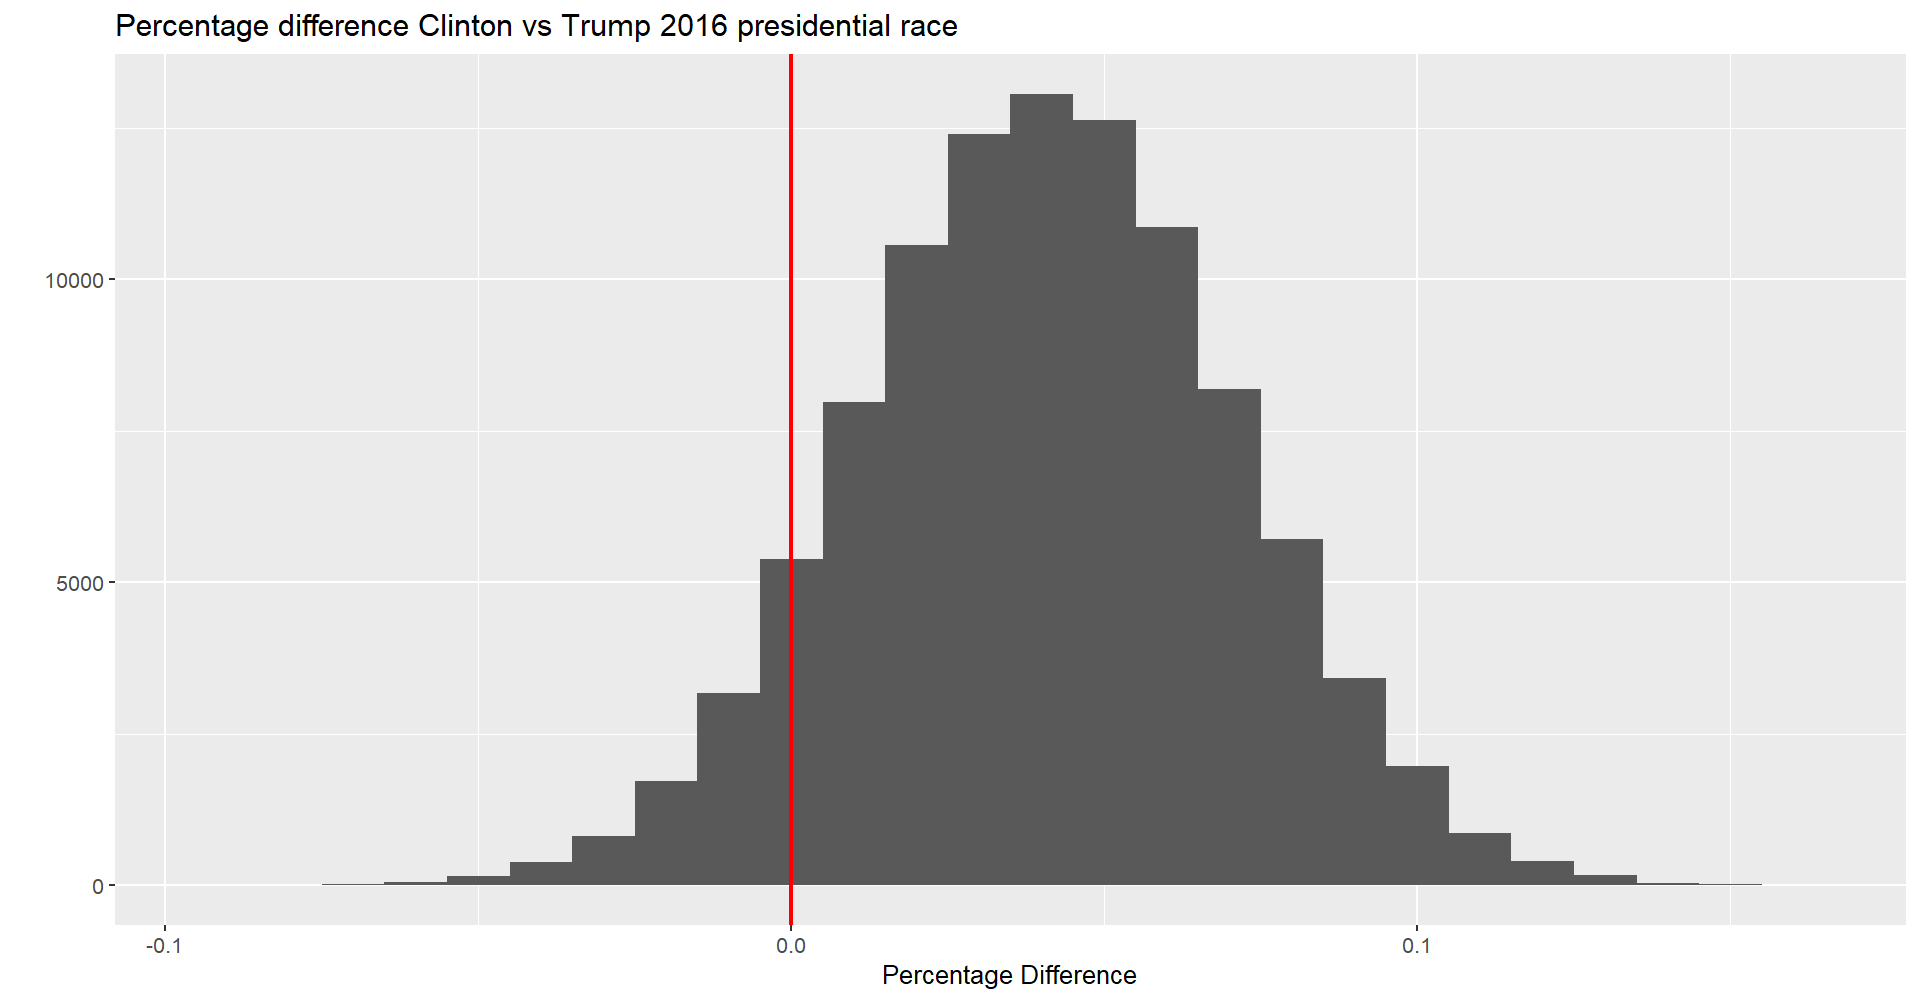
\includegraphics[width=340pt, height=200pt]{Chapters/chapter4/figures/hiillaryVStrump.png}
	%%\centerline{\epsfig{/Chapters/chapter1/figures/cat.eps,width=.8\textheight,height=.4\textwidth}}
	\caption[List of figure caption goes here]{Percentage difference: Hillary Clinton vs Donald Trump, five-way race.}\label{fig41}
\end{figure}

There is a 95\% probability that the percentage difference between Hillary and Trump according to this poll is (-1.8\%, 9.9\%). The probability of Hillary having more supporters is 91.3\%


\begin{tcolorbox}[enhanced,width=4.67in,center upper,
	fontupper=\large\bfseries,drop shadow southwest,sharp corners]
	\textit{R code. Multinomial-Dirichlet model: Polling 2016 USA presidential race}
\begin{VF}
\begin{lstlisting}[language=R]
# Predictive distribution by simulation
y0 <- c(44, 40, 16)
Pred <- apply(thetas, 1, function(p) {rmultinom(1, size = sum(y0), prob = p)})
sum(sapply(1:S, function(s) {sum(Pred[,s] == y0) == 3}))/S
0.00825
# Predictive distribution by analytical expression
PredY0 <- function(y0){
	n <- sum(y0)
	Res1 <- sum(sapply(1:length(y), function(l){lgamma(alphan[l]+y0[l]) - lgamma(alphan[l])-lfactorial(y0[l])}))
	Res <- lfactorial(n)+lgamma(sum(alphan))-lgamma(sum(alphan)+n) + Res1
	return(exp(Res))
}
PredY0(y0)
0.00850         
\end{lstlisting}
\end{VF}
\end{tcolorbox} 

The probability that from one hundred random selected people 44 support Hillary, 40 support Trump and 16 support other candidate is 0.85\%.

\item \textbf{Math test example continues}

You have a random sample of math scores of size $N=50$ from a normal distribution, $Y_i\sim \mathcal{N}(\mu, \sigma)$. The sample mean and variance are equal to $102$ and $10$, respectively. Using the normal-normal/inverse-gamma model where $\mu_0=100$, $\beta_0=1$, $\alpha_0=\delta_0=0.001$

\begin{itemize}
	\item Get 95\% confidence and credible intervals for $\mu$.
	\item What is the posterior probability that $\mu > 103$?  
\end{itemize}  

{\textbf{Answer}}

\begin{tcolorbox}[enhanced,width=4.67in,center upper,
	fontupper=\large\bfseries,drop shadow southwest,sharp corners]
	\textit{R code. Math test example continues}
\begin{VF}
\begin{lstlisting}[language=R]
set.seed(010101)
N <- 50
# Sample size
muhat <- 102
# Sample mean
sig2hat <- 10
# Sample variance
# Hyperparameters
mu0 <- 100
beta0 <- 1
delta0 <- 0.001
alpha0 <- 0.001
S <- 100000
# Posterior draws
alphan <- alpha0 + N
deltan <- sig2hat*(N - 1) + delta0 + beta0*N/(beta0 + N)*(muhat - mu0)^2
sig2Post <- invgamma::rinvgamma(S, shape = alphan, rate = deltan)
summary(sig2Post)
betan <- beta0 + N
mun <- (beta0*mu0 + N*muhat)/betan
muPost <- sapply(sig2Post, function(s2){rnorm(1, mun, sd = (s2/betan)^0.5)})
muPostq <- quantile(muPost, c(0.025, 0.5, 0.975))
muPostq
   2.5%      50%    97.5% 
101.0929 101.9625 102.8311
cutoff <- 103
PmuPostcutoff <- mean(muPost > cutoff)
PmuPostcutoff
0.00994
# Using Student's t
muPost_t <- ((deltan/(alphan*betan))^0.5)*rt(S, alphan) + mun
c1 <- rgb(173,216,230,max = 255, alpha = 50, names = "lt.blue")
c2 <- rgb(255,192,203, max = 255, alpha = 50, names = "lt.pink")
hist(muPost, main = "Histogram: Posterior mean", xlab = "Posterior mean", col = c2)
hist(muPost_t, main = "Histogram: Posterior mean", xlab = "Posterior mean", add = T, col = c1)
muPost_tq <- quantile(muPost_t, c(0.025, 0.5, 0.975))
muPost_tq
2.5%      50%    97.5% 
101.0837 101.9608 102.8435
PmuPost_tcutoff <- mean(muPost_t > cutoff)
PmuPost_tcutoff
0.01087
\end{lstlisting}
\end{VF}
\end{tcolorbox} 

We perform our calculations using the posterior conditional distribution, and the posterior marginal distribution. Both procedures give similar results as we can observe from Figure \ref{fig42}.

\begin{figure}[!h]
	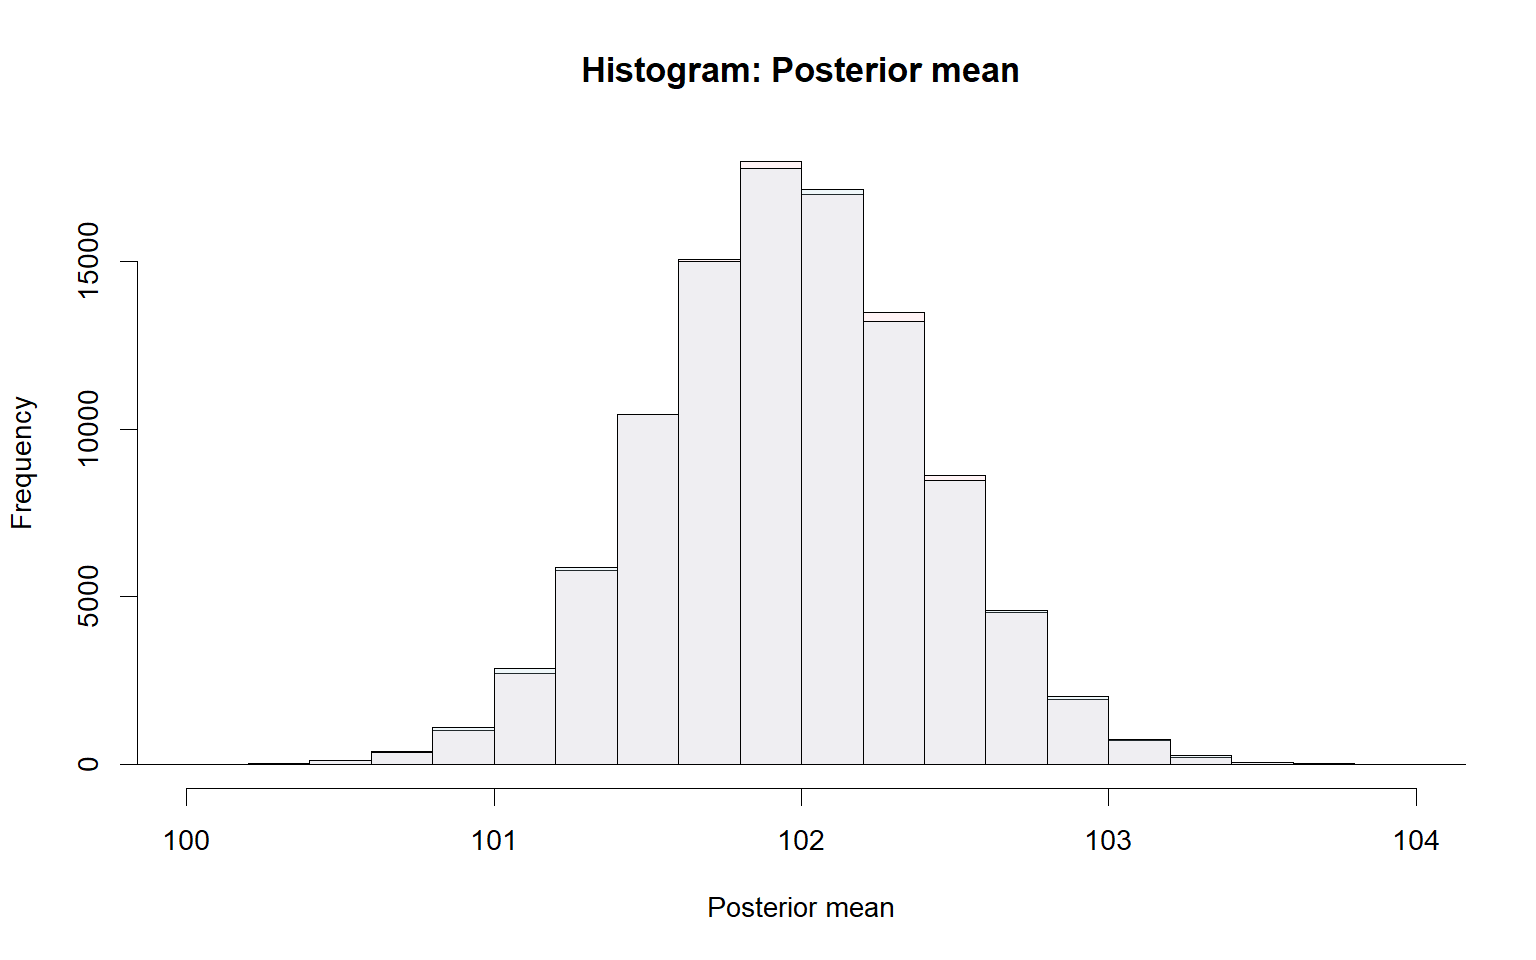
\includegraphics[width=340pt, height=200pt]{Chapters/chapter4/figures/conditionalVSmarginal.png}
	%%\centerline{\epsfig{/Chapters/chapter1/figures/cat.eps,width=.8\textheight,height=.4\textwidth}}
	\caption[List of figure caption goes here]{Histogram using the posterior conditional distribution and the posterior marginal distribution}\label{fig42}
\end{figure}


We have that the 95\% credible interval is (101.08, 102.84), and the probability of having a value greater than 103 is 1.09\%. 

%\item In the optimal tangency portfolio example, what are the equations for $\mu_{T+\kappa}=\mu_{n}$ and ${\bf\Sigma}_{T+\kappa}$? Use these equations to find the optimal weights six periods ahead using the tech stocks. 

%{\textbf{Answer}} 

\item \textbf{Demand of electricity example continues}

Set $c_0$ such that maximizes the marginal likelihood in the specifications with and without electricity price in the example of demand of electricity (empirical Bayes). Then, calculate the Bayes factor, and conclude if there is evidence supporting the inclusion of the price of electricity in the demand equation. 

{\textbf{Answer}} 

\begin{tcolorbox}[enhanced,width=4.67in,center upper,
	fontupper=\large\bfseries,drop shadow southwest,sharp corners]
	\textit{R code. Demand of electricity}
	\begin{VF}
		\begin{lstlisting}[language=R]
rm(list = ls())
set.seed(010101)
# Electricity demand
DataUt <- read.csv("https://raw.githubusercontent.com/besmarter/BSTApp/refs/heads/master/DataApp/Utilities.csv", sep = ",", header = TRUE, quote = "")
DataUtEst <- DataUt %>% 
filter(Electricity != 0)
attach(DataUtEst)
# Dependent variable: Monthly consumption (kWh) in log
Y <- log(Electricity)
N <- length(Y)
# Regressors quantity including intercept
X <- cbind(LnPriceElect, IndSocio1, IndSocio2, Altitude, Nrooms, HouseholdMem, Children, Lnincome, 1)
# Regressor without price
Xnew <- cbind(IndSocio1, IndSocio2, Altitude, Nrooms, HouseholdMem, Children, Lnincome, 1)
# Log marginal function (multiply by -1 due to minimization)
LogMarLikLM <- function(X, c0){
	k <- dim(X)[2]
	N <- dim(X)[1]	
	# Hyperparameters
	B0 <- c0*diag(k)
	b0 <- rep(0, k)
	# Posterior parameters
	bhat <- solve(t(X)%*%X)%*%t(X)%*%Y
	# Force this matrix to be symmetric
	Bn <- as.matrix(Matrix::forceSymmetric(solve(solve(B0) + t(X)%*%X))) 
	bn <- Bn%*%(solve(B0)%*%b0 + t(X)%*%X%*%bhat)
	dn <- as.numeric(d0 + t(Y)%*%Y+t(b0)%*%solve(B0)%*%b0-t(bn)%*%solve(Bn)%*%bn)
	an <- a0 + N
	# Log marginal likelihood
	logpy <- (N/2)*log(1/pi)+(a0/2)*log(d0)-(an/2)*log(dn) + 0.5*log(det(Bn)/det(B0)) + lgamma(an/2)-lgamma(a0/2)
	return(-logpy)
}
# Hyperparameters
d0 <- 0.001/2
a0 <- 0.001/2
# Empirical Bayes: Obtain c0 maximizing the log marginal likelihood
c0 <- 1000 
EB <- optim(c0, fn = LogMarLikLM, method = "Brent", lower = 0.0001, upper = 10^6, X = X)
EBnew <- optim(c0, fn = LogMarLikLM, method = "Brent", lower = 0.0001, upper = 10^6, X = Xnew)
# Change of order to take into account the -1 in the LogMarLikLM function
BFEM <- exp(EBnew$value - EB$value) 
BFEM
71897938
\end{lstlisting}
	\end{VF}
\end{tcolorbox} 

The Bayes factor based on the empirical Bayes of the model with electricity price versus the model without electricity price is equal to 71897938, this gives very strong evidence to include the price in the specification.
 
\item \textbf{Utility demand}

Use the file \textit{Utilities.csv} to estimate a multivariate linear regression model where $\mathbf{Y}_i=\left[\log(\text{electricity}_i) \ \log(\text{water}_i) \ \log(\text{gas}_i)\right]$ as function of $\log(\text{electricity price}_i)$, $\log(\text{water price}_i)$, $\log(\text{gas price}_i)$, $\text{IndSocio1}_i$, $\text{IndSocio2}_i$, $\text{Altitude}_i$, $\text{Nrooms}_i$, $\text{HouseholdMem}_i$, $\text{Children}_i$, and $\log(\text{Income}_i)$, where electricity, water and gas are monthly consumption of electricity (kWh), water (m$^3$) and gas (m$^3$), and other definitions are given in the Example of Section 4.3. Omit households that do not consume any of the utilities in this exercise. 

Set a non-informative prior framework, $\mathbf{B}_0=\left[0\right]_{11\times 3}$, $\mathbf{V}_0=1000 \mathbf{I}_{11}$, $\mathbf{\Psi}_0=1000 \mathbf{I}_{3}$ and $\alpha_0=3$, where we have $K=11$ (regressors plus intercept) and $M=3$ (equations) in this exercise.

\begin{enumerate}
	\item Find the posterior mean estimates and the highest posterior density intervals at 95\% of $\mathbf{B}$ and $\mathbf{\Sigma}$. Use the marginal distribution and the conditional distribution to obtain the posterior estimates of  $\mathbf{B}$, and compare the results.
	\item Find the Bayes factor comparing the baseline model in this exercise with the same specification but using the income in dollars. Now, calculate the Bayes factor using the income in thousand dollars. Is there any difference?
	\item Find the predictive distribution for the monthly demand of electricity, water and gas in the baseline specification of a household located in the lowest socioeconomic condition in a municipality located below 1000 meters above the sea level, 2 rooms, 3 members with children, a monthly income equal to USD 500, an electricity price equal to USD/kWh 0.15, a water price equal to USD/M$^3$ 0.70, and a gas price equal to USD/M$^3$ 0.75. 
\end{enumerate}   

{\textbf{Answer}} 

We see that the posterior estimates of the location parameters based on the marginal distribution and the conditional distribution are very similar (conditional on $\mathbf{\Sigma}$). This is important as many times there is no analytical solutions in well-known forms of marginal posterior distributions, and consequently, we should get draws of the posterior distributions based on conditional distributions of block of parameters (See Chapter \ref{chap5}).

We find that the Bayes factor of the baseline model ($\log(\text{Income})$) versus the two alternative models using income in dollars and thousand dollars are 108925764 and 0.1089261. The former gives strong evidence in favor of the baseline model, whereas the latter gives positive evidence for the model using the income in thousand dollars. This result despite that the location coefficients are the same in the two alternative specifications, except for the change in scale of the coefficients associated with income. This example shows that Bayes factors are sensitive to units of measure, and consequently, it is relevant to think carefully about the priors when performing hypothesis testing using a Bayesian framework. Observe that a nice feature in Bayesian inference is that we followed the same conceptual framework (Bayes factor) in the previous exercise and this exercise. In one hand, the previous exercise is an example of nested models, that is, one model is a restricted version of a more general model. On the other hand, this exercise is an example of non-nested models. This is not the case in the Frequentist approach. The statistical framework is not the same when testing nested and non-nested models.

\begin{tcolorbox}[enhanced,width=4.67in,center upper,
	fontupper=\large\bfseries,drop shadow southwest,sharp corners]
	\textit{R code. Utilities demand: Multivariate regression, posterior inference}
	\begin{VF}
		\begin{lstlisting}[language=R]
rm(list = ls())
set.seed(010101)
library(dplyr)
# Electricity demand
DataUt <- read.csv("https://raw.githubusercontent.com/besmarter/BSTApp/refs/heads/master/DataApp/Utilities.csv", sep = ",", header = TRUE, quote = "")
DataUtEst <- DataUt %>%  
filter(Electricity != 0 & Water !=0 & Gas != 0)
attach(DataUtEst)
Y <- cbind(log(Electricity), log(Water), log(Gas))
X <- cbind(LnPriceElect, LnPriceWater, LnPriceGas, IndSocio1, IndSocio2, Altitude, Nrooms, HouseholdMem, Children, Lnincome, 1)
M <- dim(Y)[2]
K <- dim(X)[2]
N <- dim(Y)[1]
# Hyperparameters
B0 <- matrix(0, K, M)
c0 <- 1000
V0 <- c0*diag(K)
Psi0 <- c0*diag(M)
a0 <- M
# Posterior parameters
Bhat <- solve(t(X)%*%X)%*%t(X)%*%Y 
S <- t(Y - X%*%Bhat)%*%(Y - X%*%Bhat)
Vn <- solve(solve(V0) + t(X)%*%X) 
Bn <- Vn%*%(solve(V0)%*%B0 + t(X)%*%X%*%Bhat)
Psin <- Psi0 + S + t(B0)%*%solve(V0)%*%B0 + t(Bhat)%*%t(X)%*%X%*%Bhat - t(Bn)%*%solve(Vn)%*%Bn
an <- a0 + N
#Posterior draws
s <- 10000 #Number of posterior draws
SIGs <- replicate(s, LaplacesDemon::rinvwishart(an, Psin))
BsCond <- sapply(1:s, function(s) {MixMatrix::rmatrixnorm(n = 1, mean=Bn, U = Vn,V = SIGs[,,s])})
summary(coda::mcmc(t(BsCond)))
Bs <- sapply(1:s, function(s) {MixMatrix::rmatrixt(n = 1, mean=Bn, U = Vn,V = Psin, df = an + 1 - M)})
summary(coda::mcmc(t(Bs)))
SIGMs <- t(sapply(1:s, function(l) {gdata::lowerTriangle(SIGs[,,l], diag=TRUE, byrow=FALSE)}))
summary(coda::mcmc(SIGMs))
hdiBs <- HDInterval::hdi(t(BsCond), credMass = 0.95) # Highest posterior density credible interval
hdiBs
hdiSIG <- HDInterval::hdi(SIGMs, credMass = 0.95) # Highest posterior density credible interval
hdiSIG
		\end{lstlisting}
	\end{VF}
\end{tcolorbox} 

\begin{tcolorbox}[enhanced,width=4.67in,center upper,
	fontupper=\large\bfseries,drop shadow southwest,sharp corners]
	\textit{R code. Utilities demand: Multivariate regression, Bayes factors}
	\begin{VF}
		\begin{lstlisting}[language=R]
# Log marginal function (multiply by -1 due to minimization)
LogMarLikLM <- function(X, c0){
	c10 <- c0[1]; c20 <- c0[2]
	k <- dim(X)[2]
	N <- dim(X)[1]
	# Hyperparameters
	V0 <- c10*diag(K)
	Psi0 <- c20*diag(M)
	# Posterior parameters
	Bhat <- solve(t(X)%*%X)%*%t(X)%*%Y 
	S <- t(Y - X%*%Bhat)%*%(Y - X%*%Bhat)
	Vn <- solve(solve(V0) + t(X)%*%X) 
	Bn <- Vn%*%(solve(V0)%*%B0 + t(X)%*%X%*%Bhat)
	Psin <- Psi0 + S + t(B0)%*%solve(V0)%*%B0 + t(Bhat)%*%t(X)%*%X%*%Bhat - t(Bn)%*%solve(Vn)%*%Bn
	# Log marginal likelihood
	logpy <- (N*M/2)*log(1/pi)+(a0/2)*log(det(Psi0)) - (an/2)*log(det(Psin)) + (M/2)*(log(det(Vn)) - log(det(V0))) + lgamma(an/2)-lgamma(a0/2)
	return(-logpy)
}
c0 <- rep(1000, 2)
LogML <- LogMarLikLM(X=X, c0 = c0)
# Using income in dollars as regressor
Xnew <- cbind(LnPriceElect, LnPriceWater, LnPriceGas, IndSocio1, IndSocio2, Altitude, Nrooms, HouseholdMem, Children, exp(Lnincome), 1)
LogMLnew <- LogMarLikLM(X=Xnew, c0 = c0)
# Bayes factor
BF12 <- exp(LogMLnew - LogML)
BF12
# Using income in thousand dollars as regressor
XnewT <- cbind(LnPriceElect, LnPriceWater, LnPriceGas, IndSocio1, IndSocio2, Altitude, Nrooms, HouseholdMem, Children, exp(Lnincome)/1000, 1)
LogMLnewT <- LogMarLikLM(X=XnewT, c0 = c0)
# Bayes factor
BF13 <- exp(LogMLnewT - LogML)
BF13
		\end{lstlisting}
	\end{VF}
\end{tcolorbox} 

\begin{tcolorbox}[enhanced,width=4.67in,center upper,
	fontupper=\large\bfseries,drop shadow southwest,sharp corners]
	\textit{R code. Utilities demand: Multivariate regression, predictive distribution}
	\begin{VF}
		\begin{lstlisting}[language=R]
# Predictive distribution
Xpred <- c(log(0.15), log(0.70), log(0.75), 1, 0, 0, 2, 3, 1, log(500), 1)
Mean <- Xpred%*%Bn
Hn <- 1+t(Xpred)%*%Vn%*%Xpred
UtilDemand <- exp(replicate(s, MixMatrix::rmatrixt(n = 1, mean=Mean, U = Hn, V = Psin, df = an + 1 - M)))
ElePred <- UtilDemand[1,1,]
WatPred <- UtilDemand[1,2,]
GasPred <- UtilDemand[1,3,]
data <- data.frame(cbind(ElePred, WatPred, GasPred)) #Data frame
annotations1 <- data.frame(
x = round(quantile(data$ElePred, c(0.025, 0.5, 0.975)),1),
y = c(600, 1000, 600),
label = c("2.5%:", "50%:", "97.5%:")
)
annotations2 <- data.frame(
x = round(quantile(data$WatPred, c(0.025, 0.5, 0.975)),1),
y = c(600, 1000, 600),
label = c("2.5%:", "50%:", "97.5%:")
)
annotations3 <- data.frame(
x = round(quantile(data$GasPred, c(0.025, 0.5, 0.975)),1),
y = c(600, 1000, 600),
label = c("2.5%:", "50%:", "97.5%:")
)
require(ggplot2) # Cool figures
require(ggpubr) # Multiple figures in one page
require(latex2exp) # LaTeX equations in figures
fig1 <- ggplot(data = data, aes(ElePred)) + geom_histogram(bins = 40, color = "#000000", fill = "#0099F8") + 	xlab("kWh") + ylab("Frequency") +	ggtitle("Electricity") + xlim(0, 1050) + geom_text(data = annotations1, aes(x = x, y = y, label = paste(label, x)), size = 3, fontface = "bold")
fig2 <- ggplot(data = data, aes(WatPred)) + geom_histogram(bins = 40, color = "#000000", fill = "#0099F8") + 	xlab(TeX("$M^3$")) + ylab("Frequency") +	ggtitle("Water") + xlim(0, 100) + geom_text(data = annotations2, aes(x = x, y = y, label = paste(label, x)), size = 3, fontface = "bold")
fig3 <- ggplot(data = data, aes(GasPred)) + geom_histogram(bins = 40, color = "#000000", fill = "#0099F8") + 	xlab(TeX("$M^3$")) + ylab("Frequency") +	ggtitle("Gas") + xlim(0, 80) + geom_text(data = annotations3, aes(x = x, y = y, label = paste(label, x)), size = 3, fontface = "bold")
		\end{lstlisting}
	\end{VF}
\end{tcolorbox} 


Figures \ref{fig13}, \ref{fig14} and \ref{fig15} show the marginal predictive distributions of electricity, water and gas for the reference household. The median predictive values are kWh 168.8, M$^3$ 12.3 and M$^3$ 10.1, respectively. In addition, the 95\% credible intervals are (27.7, 1028.9), (1.5, 98.7) and (1.5, 67.5) for electricity, water and gas.  

\begin{figure}[!h]
	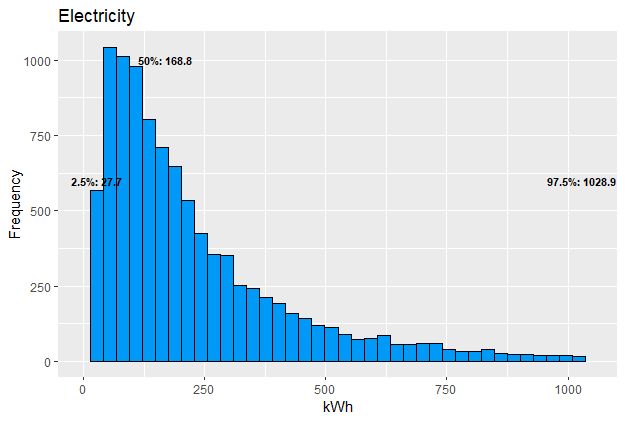
\includegraphics[width=340pt, height=200pt]{Chapters/chapter4/figures/ElectMulti.png}
	%%\centerline{\epsfig{/Chapters/chapter1/figures/cat.eps,width=.8\textheight,height=.4\textwidth}}
	\caption[List of figure caption goes here]{Histogram using the posterior predictive distribution of electricity demand}\label{fig13}
\end{figure}

\begin{figure}[!h]
	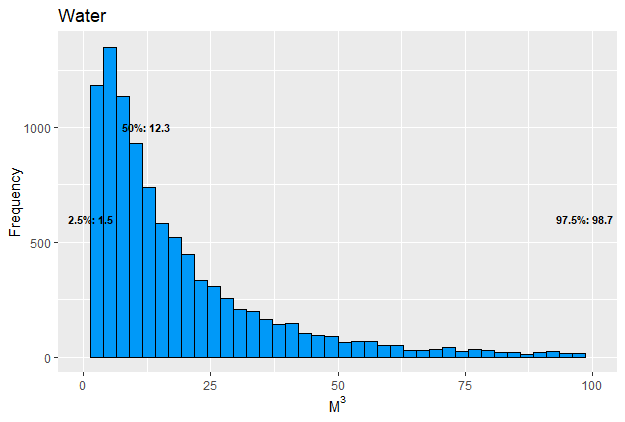
\includegraphics[width=340pt, height=200pt]{Chapters/chapter4/figures/WaterMulti.png}
	%%\centerline{\epsfig{/Chapters/chapter1/figures/cat.eps,width=.8\textheight,height=.4\textwidth}}
	\caption[List of figure caption goes here]{Histogram using the posterior predictive distribution of water demand}\label{fig14}
\end{figure}  

\begin{figure}[!h]
	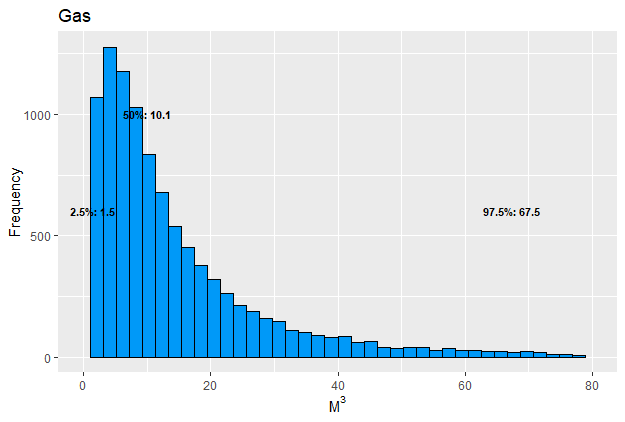
\includegraphics[width=340pt, height=200pt]{Chapters/chapter4/figures/GasMulti.png}
	%%\centerline{\epsfig{/Chapters/chapter1/figures/cat.eps,width=.8\textheight,height=.4\textwidth}}
	\caption[List of figure caption goes here]{Histogram using the posterior predictive distribution of gas demand}\label{fig15}
\end{figure}    
\end{enumerate}




\chapter{Simulation methods}\label{chap5}

In the previous chapters, we focused on conjugate families, where the posterior and predictive distributions have standard analytical forms (e.g., normal, Student's t, gamma, binomial, Poisson, etc.) and where the marginal likelihood has a closed-form analytical solution. However, realistic models are often more complex and lack such closed-form solutions.

To address this complexity, we rely on simulation (stochastic) methods to draw samples from posterior and predictive distributions. This chapter introduces posterior simulation, a cornerstone of Bayesian inference. We discuss Markov Chain Monte Carlo (MCMC) methods, including Gibbs sampling, Metropolis-Hastings, and Hamiltonian Monte Carlo, as well as other techniques like importance sampling and sequential Monte Carlo.

The simulation methods discussed in this chapter are specifically applied throughout this book. However, we do not delve into deterministic methods, such as numerical integration (quadrature), or other simulation methods, including discrete approximation, the probability integral transform, the method of composition, accept-reject sampling, and slice sampling algorithms. While these methods are also widely used, they are not as common as the approaches explicitly employed in this book.

For readers interested in these alternative methods, we recommend exploring \cite[Chaps.~2 and 3]{robert2010introducing}, \cite[Chaps.~2, 3, and 8]{robert2011monte}, \cite[Chap.~5]{greenberg2012introduction}, and \cite[Chap.~10]{gelman2021bayesian}.

%\section{The inverse transform method}\label{sec51}

%\section{Method of composition}\label{sec52}

%\section{Accept and reject algorithm}\label{sec53}

\section{Markov chain Monte Carlo methods}\label{sec51}

Markov Chain Monte Carlo (MCMC) methods are algorithms used to approximate complex probability distributions by constructing a Markov chain. This chain is a sequence of random samples where each sample depends only on the previous one. The goal of MCMC methods is to obtain draws from the posterior distribution as the equilibrium distribution. The key point in MCMC methods is the transition kernel or density, $\pi(\bm{\theta}^{(s)}|\bm{\theta}^{(s-1)})$, which generates a draw $\bm{\theta}^{(s)}$ at stage $s$ that depends solely on $\bm{\theta}^{(s-1)}$. This transition distribution must be designed such that the Markov chain converges to a unique stationary distribution, which, in our case, is the posterior distribution, that is, $\pi(\bm{\theta}^{(s)}|\bm{y})=\int_{\bm{\Theta}}\pi(\bm{\theta}^{(s)}|\bm{\theta}^{(s-1)},\bm{y})\pi(\bm{\theta}^{(s-1)}|\bm{y})d\bm{\theta}^{(s-1)}$.

Given that we start at an arbitrary point, $\bm{\theta}^{(0)}$, the algorithm requires that the Markov chain be \textit{irreducible}, meaning that the process can reach any other state with positive probability. Additionally, the process must be \textit{aperiodic}, meaning that for each state, the greatest common divisor of the number of steps it takes to return to the state is 1, ensuring that there are no cycles forcing the system to return to a state only after a fixed number of steps. Furthermore, the process must be \textit{recurrent}, meaning that it will return to any state an infinite number of times with probability one. However, to ensure convergence to the stationary distribution, a stronger condition is required: the process must be \textit{positive recurrent}, meaning that the expected return time to a state is finite. Given an \textit{irreducible}, \textit{aperiodic}, and \textit{positive recurrent} transition density, the Markov chain algorithm will asymptotically converge to the stationary posterior distribution we are seeking. For more details, see \cite[chap.~6]{robert2011monte}.
   

%\subsection{Some theory}\label{sec551}

\subsection{Gibbs sampler}\label{sec511}

This Gibbs sampler algorithm is one of the most widely used MCMC methods for sampling from non-standard distributions in Bayesian analysis. While it is a special case of the Metropolis-Hastings (MH) algorithm, it originated from a different theoretical background \cite{Geman1984}. The key requirement for implementing the Gibbs sampling algorithm is the availability of conditional posterior distributions. The algorithm works by cycling through the conditional posterior distributions corresponding to different blocks of the parameter space under inference.

Two simplify concepts let's focus on a parameter space composed by two blocks, $\bm{\theta} = [\bm{\theta}_1 \ \bm{\theta}_2]^{\top}$, the Gibbs sampling algorithm uses as transition kernel $\pi(\bm{\theta}_1^{(s)},\bm{\theta}_2^{(s)}|\bm{\theta}_1^{(s-1)},\bm{\theta}_2^{(s-1)},\bm{y})=\pi(\bm{\theta}_1^{(s)}|\bm{\theta}_2^{(s-1)},\bm{y})\pi(\bm{\theta}_2^{(s)}|\bm{\theta}_1^{(s)},\bm{y})$. Thus,
{\scriptsize
\begin{align*}
	\int_{\bm{\Theta}}\pi(\bm{\theta}^{(s)}|\bm{\theta}^{(s-1)},\bm{y})\pi(\bm{\theta}^{(s-1)}|\bm{y})d\bm{\theta}^{(s-1)}
	&=\int_{\bm{\Theta}_2}\int_{\bm{\Theta}_1}\pi(\bm{\theta}_1^{(s)}|\bm{\theta}_2^{(s-1)},\bm{y})\pi(\bm{\theta}_2^{(s)}|\bm{\theta}_1^{(s)},\bm{y})\pi(\bm{\theta}^{(s-1)}_1,\bm{\theta}^{(s-1)}_2|\bm{y})d\bm{\theta}^{(s-1)}_1d\bm{\theta}^{(s-1)}_2\\
	&=\pi(\bm{\theta}_2^{(s)}|\bm{\theta}_1^{(s)},\bm{y})\int_{\bm{\Theta}_2}\int_{\bm{\Theta}_1}\pi(\bm{\theta}_1^{(s)}|\bm{\theta}_2^{(s-1)},\bm{y})\pi(\bm{\theta}^{(s-1)}_1,\bm{\theta}^{(s-1)}_2|\bm{y})d\bm{\theta}^{(s-1)}_1d\bm{\theta}^{(s-1)}_2\\
	&=\pi(\bm{\theta}_2^{(s)}|\bm{\theta}_1^{(s)},\bm{y})\int_{\bm{\Theta}_2}\pi(\bm{\theta}_1^{(s)}|\bm{\theta}_2^{(s-1)},\bm{y})\pi(\bm{\theta}^{(s-1)}_2|\bm{y})d\bm{\theta}^{(s-1)}_2\\
	&=\pi(\bm{\theta}_2^{(s)}|\bm{\theta}_1^{(s)},\bm{y})\int_{\bm{\Theta}_2}\pi(\bm{\theta}_1^{(s)},\bm{\theta}_2^{(s-1)}|\bm{y})d\bm{\theta}^{(s-1)}_2\\
	&=\pi(\bm{\theta}_2^{(s)}|\bm{\theta}_1^{(s)},\bm{y})\pi(\bm{\theta}_1^{(s)}|\bm{y})\\
	&=\pi(\bm{\theta}_1^{(s)},\bm{\theta}_2^{(s)}|\bm{y}).\\
\end{align*}
}
Then, $\pi(\bm{\theta}|\bm{y})$ is the stationary distribution for the Gibbs transition kernel.

A word of caution! Even if we have well-defined conditional posterior distributions $\pi(\bm{\theta}_1^{(s)} \mid \bm{\theta}_2^{(s-1)}, \bm{y})$ and $\pi(\bm{\theta}_2^{(s)} \mid \bm{\theta}_1^{(s)}, \bm{y})$, and we can simulate from them, the joint posterior distribution $\pi(\bm{\theta}_1^{(s)}, \bm{\theta}_2^{(s)} \mid \bm{y})$ may not correspond to any proper distribution. We should be mindful of this situation, especially when dealing with improper prior distributions (see \cite[Chap.~10]{robert2011monte} for details).

Algorithm \ref{Alg:Gibbs} shows how to implement a Gibbs sampler with $d$ blocks. 

\begin{algorithm}[h!]
	\caption{Gibbs sampling}\label{Alg:Gibbs}
	\begin{algorithmic}[1]  		 			
		\State Set $\bm{\theta}_2^{(0)}$, $\bm{\theta}_3^{(0)}$, ..., $\bm{\theta}_d^{(0)}$
		\For{\texttt{$s=1,\dots,S$}}
		\State Draw $\bm{\theta}_1^{(s)}$ from $\pi(\bm{\theta}_1^{(s)}|\bm{\theta}_2^{(s-1)},\dots,\bm{\theta}_d^{(s-1)})$
		\State Draw $\bm{\theta}_2^{(s)}$ from $\pi(\bm{\theta}_2^{(s)}|\bm{\theta}_1^{(s)},\dots,\bm{\theta}_d^{(s-1)})$
		\State $\vdots$
		\State Draw $\bm{\theta}_d^{(s)}$ from $\pi(\bm{\theta}_d^{(s)}|\bm{\theta}_2^{(s)},\dots,\bm{\theta}_{d-1}^{(s)})$ 
		\EndFor 
		\end{algorithmic} 
\end{algorithm}

\textbf{Example: The normal model with independent priors}

Let's recap the math test exercise in Chapter \ref{chap4}, this time assuming independent priors. Specifically, let $Y_i \sim N(\mu, \sigma^2)$, where $\mu \sim N(\mu_0, \sigma_0^2)$ and $\sigma^2 \sim IG(\alpha_0 / 2, \delta_0 / 2)$. The sample size is 50, and the mean and standard deviation of the math scores are 102 and 10, respectively. We set $\mu_0 = 100$, $\sigma_0^2 = 100$, and $\alpha_0 = \delta_0 = 0.001$.

The posterior distribution is
\begin{align*}
	\pi(\mu,\sigma^2|\bm{y})&\propto (\sigma^2)^{-N/2}\exp\left\{-\frac{1}{2\sigma^2}\sum_{i=1}^N(y_i-\mu)^2\right\}\\
	&\times \exp\left\{-\frac{1}{2\sigma^2_0}(\mu-\mu_0)^2\right\}\times \left(\frac{1}{\sigma^2}\right)^{\alpha_0/2+1}\exp\left\{-\frac{\delta_0}{2\sigma^2}\right\}.
\end{align*}
Thus, the conditional posterior distribution of $\mu$ is
\begin{align*}
	\pi(\mu,\sigma^2|\bm{y})&\propto \exp\left\{-\frac{1}{2}\left[\frac{1}{\sigma^2}\sum_{i=1}^N(y_i-\mu)^2+\frac{1}{\sigma^2_0}(\mu-\mu_0)^2\right]\right\}\\
	&\propto \exp\left\{-\frac{1}{2}\left[\mu^2\left(\frac{1}{\sigma^2/N}+\frac{1}{\sigma^2_0}\right)-2\mu\left(\frac{\bar{y}}{\sigma^2/N}+\frac{\mu_0}{\sigma_0^2}\right)\right]\right\}.  
\end{align*} 
We set $\mu_n=\sigma^{2}_n\left(\frac{\bar{y}}{\sigma^2/N}+\frac{\mu_0}{\sigma_0^2}\right)$ and $\sigma^{2}_n=\left(\frac{1}{\sigma^2/N}+\frac{1}{\sigma_0^2}\right)^{-1}$. Thus,
\begin{align*}
	\pi(\mu,\sigma^2|\bm{y})&\propto \exp\left\{-\frac{1}{2\sigma_n^2}\left[\mu^2-2\mu\mu_n+\mu_n^2-\mu_n^2\right]\right\}\\
	&\propto \exp\left\{-\frac{1}{2\sigma_n^2}(\mu-\mu_n)^2\right\}.\\  
\end{align*} 
This is the kernel of a normal distribution, that is, $\mu|\sigma^2,\bm{y}\sim N(\mu_n,\sigma_n^2)$.

The conditional posterior distribution of $\sigma^2$ is given by
\begin{align*}
	\pi(\sigma^2|\mu,\bm{y})&\propto (\sigma^2)^{-N/2}\exp\left\{-\frac{1}{2\sigma^2}\sum_{i=1}^N(y_i-\mu)^2\right\}\\
	&\times \left(\frac{1}{\sigma^2}\right)^{\alpha_0/2+1}\exp\left\{-\frac{\delta_0}{2\sigma^2}\right\}\\
	&\propto (\sigma^2)^{-N/2-\alpha_0/2-1} \exp\left\{-\frac{1}{2\sigma^2}\left[\sum_{i=1}^N(y_i-\mu)^2+\delta_0\right]\right\}.
\end{align*} 
Thus, $\sigma^2|\mu,\bm{y}\sim IG(\alpha_n/2,\delta_n/2)$, where $\alpha_n=N+\alpha_0$ and $\delta_n=\sum_{i=1}^N(y_i-\mu)^2+\delta_0=N\hat{\sigma}^2+N(\bar{y}-\mu)^2+\delta_0$ given that $\sum_{i=1}^N(y_i-\bar{y})=0$, where $\bar{y}$ and $\hat{\sigma}$ are the mean and standard deviation estimates.

As we have the conditional posterior distributions, we can use the Gibbs sampling algorithm to perform inference in this model. The following code shows how to do it.

\begin{tcolorbox}[enhanced,width=4.67in,center upper,
	fontupper=\large\bfseries,drop shadow southwest,sharp corners]
	\textit{R code. Gibbs sampler: The math example}
	\begin{VF}
		\begin{lstlisting}[language=R]
rm(list = ls()); set.seed(010101)
N <- 50 # Sample size
muhat <- 102 # Sample mean
sig2hat <- 100 # Sample variance
# Hyperparameters
mu0 <- 100; sig20 <- 100; delta0 <- 0.001; alpha0 <- 0.001
# MCMC parameters
MCMC <- 10000; burnin <- 1000; S <- MCMC + burnin
keep <- (burnin+1):S
# Posterior draws
sig2Post <- rep(NA, S)
muPost <- rep(NA, S)
alphan <- alpha0 + N; sig2 <- sig20
# Gibbs sampler
for(s in 1:S){
	sig2n <- (1/(sig2/N)+1/sig20)^(-1)
	mun <- sig2n*(muhat/(sig2/N)+mu0/sig20)
	mu <- rnorm(1, mun, sig2n^0.5)
	deltan <- N*(sig2hat + (muhat - mu)^2)
	sig2 <- invgamma::rinvgamma(1, shape = alphan, rate = deltan)
	muPost[s] <- mu;sig2Post[s] <- sig2
}
sig2s <- coda::mcmc(sig2Post[keep]) 
mus <- coda::mcmc(muPost[keep]) 
summary(sig2s); summary(mus)
hist(mus, main = "Histogram: Posterior mean", xlab = "Posterior mean", col = "blue", breaks = 50)
muPost_tq <- quantile(mus, c(0.025, 0.5, 0.975)); muPost_tq
PmuPost_tcutoff <- mean(mus > 102); PmuPost_tcutoff
\end{lstlisting}
	\end{VF}
\end{tcolorbox} 

\begin{figure}[!h]
	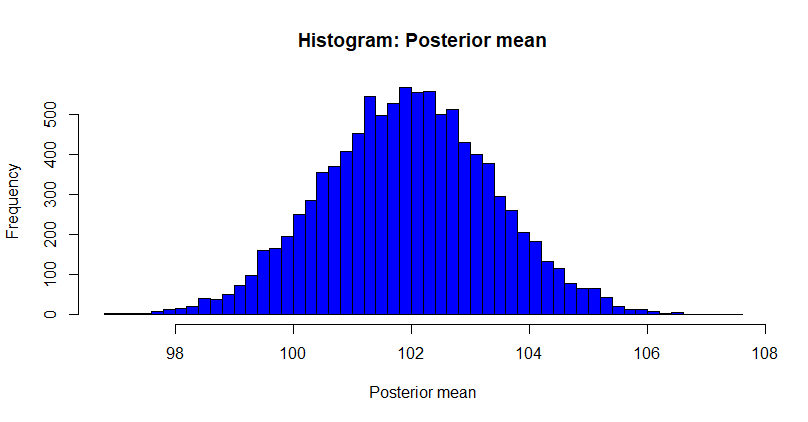
\includegraphics[width=340pt, height=200pt]{Chapters/chapter5/figures/PostMeanMathTest.png}
	%%\centerline{\epsfig{/Chapters/chapter1/figures/cat.eps,width=.8\textheight,height=.4\textwidth}}
	\caption[List of figure caption goes here]{Histogram of posterior draws of mean: Math test}\label{fig51}
\end{figure}

Figure \ref{fig51} shows the histogram of the draws of the posterior mean of the math test results. The posterior mean and median are 101.94 and 101.95, and the 95\% credible interval is (99.14, 104.79).\\


\textbf{Example: Mining disaster change point}

Let's use the dataset \textit{Mining.csv} provided by \cite{carlin1992hierarchical}.This dataset counts mining disasters per year from 1851 to 1962 in British coal mines. 

We assume that there is an unknown structural change point in the amount of mining disasters where the parameters of the Poisson distributions describing change. In particular,
\begin{align*}
	p(y_t)=\begin{Bmatrix}
		\frac{\exp(-\lambda_1)\lambda_1^{y_t}}{y_t!}, & t=1,2,\dots,H\\
		\frac{\exp(-\lambda_2)\lambda_2^{y_t}}{y_t!}, & t=H+1,\dots,T\\
	\end{Bmatrix},
\end{align*}  
where $H$ is the changing point.

We use conjugate families for $\lambda_l$, $l=1,2$, that is, $\lambda_l\sim G(\alpha_{l0},\delta_{l0})$, and set $\pi(H)=1/T$, that is, an discrete uniform distribution for the changing point. 

\textbf{Example: Linear regression electricity demand}
Let's recap the electricity demand example in Chapter \ref{chap4}.  

\textbf{Example: Multivariate normal model, utility demand}
Let's recap the utility demand exercise in Chapter \ref{chap4}. 



\subsection{Metropolis-Hastings}\label{sec512}

\section{Importance sampling}\label{sec52}

\section{Sequential Monte Carlo}\label{sec53}

\section{Hamiltonian Monte Carlo}\label{sec54}

\section{Convergence diagnostics}\label{sec55}
\subsection{Numerical standard error}
\subsection{Effective sample size}
\subsection{Checking for errors in the posterior simulator}
\cite{geweke2004getting}
\part{Regression models: A GUIded tour}
\chapter{Univariate models}\label{chap6}

We describe how to perform Bayesian inference in some of the most common univariate models: normal-inverse gamma, logit, probit, multinomial probit and logit, ordered probit, negative binomial, tobit, quantile regression, and Bayesian bootstrap in linear models. The point of departure is assuming a random sample of cross-sectional units. Then, we show the posterior distributions of the parameters and some applications. In addition, we show how to perform inference in various models using three levels of programming skills: our graphical user interface (GUI), packages from \textbf{R}, and programming the posterior distributions. The first requires no programming skills, the second requires an intermediate level, and the third demands more advanced skills. We also include mathematical and computational exercises.

We can run our GUI typing

\begin{tcolorbox}[enhanced,width=4.67in,center upper,
	fontupper=\large\bfseries,drop shadow southwest,sharp corners]
	\textit{R code. How to display our graphical user interface}
	\begin{VF}
		\begin{lstlisting}[language=R]
	shiny::runGitHub("besmarter/BSTApp", launch.browser = T)
\end{lstlisting}
	\end{VF}
\end{tcolorbox} 

in the \textbf{R} package console or any \textbf{R} code editor. However, users should see Chapter \ref{chapGUI} for details.

\section{The Gaussian linear model}\label{sec61}

The Gaussian linear model specifies ${\bf{y}}={\bf{X}}\bm{\bm{\beta}}+\bm{\mu}$ such that $\bm{\mu}\sim N(\bf{0},\sigma^2\bf{I}_N)$ is an stochastic error, ${\bf{X}}$ is a $N \times K$ matrix of regressors, $\bm{\bm{\beta}}$ is a $K$-dimensional vector of location coefficients, $\sigma^2$ is the variance of the model (scale parameter), ${\bf{y}}$ is a $N$-dimensional vector of a dependent variable, and $N$ is the sample size. We describe this model using the conjugate family in Section \ref{sec43}, that is, $\pi(\bm{\bm{\beta}},\sigma^2)=\pi(\bm{\bm{\beta}}|\sigma^2)\times\pi(\sigma^2)$, and this allowed to get the posterior marginal distribution for $\bm{\bm{\beta}}$ and $\sigma^2$.

We assume independent prior in this section, that is, $\pi(\bm{\beta},\sigma^2)=\pi(\bm{\beta})\times\pi(\sigma^2)$, where $\bm{\beta} \sim N(\bm{\beta}_0, {\bf{B}}_0)$ and $\sigma^2 \sim IG(\alpha_0/2, \delta_0/2)$, $\alpha_0/2$ and $\delta_0/2$ are the shape and rate parameters. This setting allows getting the posterior conditional distributions, that is, $\pi(\bm{\beta}|\sigma^2,{\bf{y}}, {\bf{X}})$ and $\pi(\sigma^2|\bm{\beta},{\bf{y}}, {\bf{X}})$, which in turn allows to use the Gibbs sampler algorithm to perform posterior inference of $\bm{\beta}$ and $\sigma^2$.

The likelihood function in this model is
\begin{align*}
	p({\bf{y}}| \bm{\beta}, \sigma^2, {\bf{X}}) = (2\pi\sigma^2)^{-\frac{N}{2}} \exp \left\{-\frac{1}{2\sigma^2} ({\bf{y}} - \bf{X\bm{\beta}})^{\top}({\bf{y}} - \bf{X\bm{\beta}}) \right\}.
\end{align*}

Then, the conditional posterior distributions are

\begin{align*}
	\bm{\beta}|\sigma^2, {\bf{y}}, {\bf{X}} \sim N(\bm{\beta}_n, \sigma^2{\bf{B}}_n),
\end{align*}
and
\begin{align*}
	\sigma^2|\bm{\beta}, {\bf{y}}, {\bf{X}} \sim IG(\alpha_n/2, \delta_n/2),
\end{align*}

 where ${\bf{B}}_n = ({\bf{B}}_0^{-1} + \sigma^{-2} {\bf{X}}^{\top}{\bf{X}})^{-1}$, $\bm{\beta}_n= {\bf{B}}_n({\bf{B}}_0^{-1}\bm{\beta}_0 + \sigma^{-2} {\bf{X}}^{\top}{\bf{y}})$, $\alpha_n = \alpha_0 + N$ and $\delta_n = \delta_0 + ({\bf{y}}-{\bf{X}}\bm{\beta})^{\top}({\bf{y}}-{\bf{X}}\bm{\beta})$ (see Exercise 1 in this chapter).\footnote{This model can be extended to consider heteroskedasticity such that $y_i\sim N({\bf{x}}_i^{\top}\bm{\beta}, \sigma^2/\tau_i)$, where $\tau_i\sim G(v/2,v/2)$. See exercise 2 for details.}\\

\textbf{Example: The market value of soccer players in Europe}

Let's analyze the determinants of the market value of soccer players in Europe. In particular, we use the dataset \textit{1ValueFootballPlayers.csv} which is in folder \textbf{DataApp} in our github repository \textbf{https://github.com/besmarter/BSTApp}. This dataset was used by \cite{Serna2018} to finding the determinants of high performance soccer players in the five most important national leagues in Europe.

The specification of the model is
\begin{align*}
	\log(\text{Value}_i)&={\beta}_1+{\beta}_2\text{Perf}_i+{\beta}_3\text{Age}_i+{\beta}_4\text{Age}^2_i+{\beta}_5\text{NatTeam}_i\\
	&+{\beta}_6\text{Goals}_i+{\beta}_7\text{Exp}_i+{\beta}_{8}\text{Exp}^2_i+\mu_i,
\end{align*}

where \textit{Value} is the market value in Euros (2017), \textit{Perf} is a measure of performance, \textit{Age} is the players' age in years, \textit{NatTem} is an indicator variable that takes the value of 1 if the player has been on the national team, \textit{Goals} is the number of goals scored by the player during his career, and \textit{Exp} is his experience in years.  

We assume that the dependent variable distributes normal, then we use a normal-inverse gamma model using vague conjugate priors where ${\bf{B}}_0=1000{\bf{I}}_{8}$, $\bm{\beta}_0={\bf{0}}_{8}$, $\alpha_0=0.001$ and $\delta_0=0.001$. We perform a Gibbs sampler with 5,000 MCMC iterations plus a burn-in equal to 5,000, and a thinning parameter equal to 1.

Once our GUI is displayed (see beginning of this chapter), we should follow Algorithm \ref{alg:Gaussian} to run linear Gaussian models in our GUI (see Chapter \ref{chapGUI} for details):
\begin{algorithm}[h!]
	\caption{Linear Gaussian model}\label{alg:Gaussian}
	\begin{algorithmic}[1]  		 			
		\State Select \textit{Univariate Models} on the top panel
		\State Select \textit{Normal} model using the left radio button
		\State Upload the dataset selecting first if there is header in the file, and the kind of separator in the \textit{csv} file of the dataset (comma, semicolon, or tab). Then, use the \textit{Browse} button under the \textbf{Choose File} legend. You should see a preview of the dataset
		\State Select MCMC iterations, burn-in and thinning parameters using the \textit{Range sliders}
		\State Select dependent and independent variables using the \textit{Formula builder} table
		\State Click the \textit{Build formula} button to generate the formula in \textbf{R} syntax. You can modify the formula in the \textbf{Main equation} box using valid arguments of the \textit{formula} command structure in \textbf{R}
		\State Set the hyperparameters: mean vector, covariance matrix, shape and scale parameters. This step is not necessary as by default our GUI uses non-informative priors
		\State Click the \textit{Go!} button
		\State Analyze results
		\State Download posterior chains and diagnostic plots using the \textit{Download Posterior Chains} and \textit{Download Posterior Graphs} buttons
	\end{algorithmic} 
\end{algorithm}

We can see in the next \textbf{R} codes how to perform the linear Gaussian model using the command \textit{MCMCregress} of the \textit{MCMCpack} package, and programming the Gibbs sampler ourselves. We should get similar results using the three approaches: GUI, package and our function. In fact, our GUI relies on the \textit{MCMCregress} command. For instance, the value of a top soccer player in Europe increases 134\% ($\exp(0.85)-1)$) on average when he has played in the national team, the credible interval at 95\% is (86\%, 197\%).  


\begin{tcolorbox}[enhanced,width=4.67in,center upper,
	fontupper=\large\bfseries,drop shadow southwest,sharp corners]\label{code1}
	\textit{R code. The value of soccer players, using \textbf{R} packages}
	\begin{VF}
		\begin{lstlisting}[language=R]		
rm(list = ls())
set.seed(010101)
########################## Linear regression: Value of soccer players ##########################
Data <- read.csv("https://raw.githubusercontent.com/besmarter/BSTApp/refs/heads/master/DataApp/1ValueFootballPlayers.csv", sep = ",", header = TRUE, quote = "")
attach(Data)
y <- log(Value) 
# Value: Market value in Euros (2017) of soccer players
# Regressors quantity including intercept
X <- cbind(1, Perf, Age, Age2, NatTeam, Goals, Exp, Exp2)
# Perf: Performance. Perf2: Performance squared. Age: Age; Age: Age squared. 
# NatTeam: Indicator of national team. Goals: Scored goals. Goals2: Scored goals squared
# Exp: Years of experience. Exp2: Years of experience squared. Assists: Number of assists
k <- dim(X)[2]
N <- dim(X)[1]
# Hyperparameters
d0 <- 0.001/2
a0 <- 0.001/2
b0 <- rep(0, k)
c0 <- 1000
B0 <- c0*diag(k)
B0i <- solve(B0)
# MCMC parameters
mcmc <- 5000
burnin <- 5000
tot <- mcmc + burnin
thin <- 1
# Posterior distributions using packages: MCMCpack sets the model in terms of the precision matrix
posterior  <- MCMCpack::MCMCregress(y~X-1, b0=b0, B0 = B0i, c0 = a0, d0 = d0, burnin = burnin, mcmc = mcmc, thin = thin)
summary(coda::mcmc(posterior))
Iterations = 1:5000
Thinning interval = 1 
Number of chains = 1 
Sample size per chain = 5000 
1. Empirical mean and standard deviation for each variable,
plus standard error of the mean:
					Mean       SD  Naive SE Time-series SE
X         3.695499 2.228060 3.151e-02      3.151e-02
XPerf     0.035445 0.004299 6.079e-05      6.079e-05
XAge      0.778410 0.181362 2.565e-03      2.565e-03
XAge2    -0.016617 0.003380 4.781e-05      4.781e-05
XNatTeam  0.850362 0.116861 1.653e-03      1.689e-03
XGoals    0.009097 0.001603 2.266e-05      2.266e-05
XExp      0.206208 0.062713 8.869e-04      8.428e-04
XExp2    -0.006992 0.002718 3.844e-05      3.719e-05
sigma2    0.969590 0.076091 1.076e-03      1.076e-03
\end{lstlisting}
	\end{VF}
\end{tcolorbox} 

\begin{tcolorbox}[enhanced,width=4.67in,center upper,
	fontupper=\large\bfseries,drop shadow southwest,sharp corners]
	\textit{R. code. The value of soccer players, programming our Gibbs sampler}
	\begin{VF}
		\begin{lstlisting}[language=R]		
# Posterior distributions programming the Gibbs sampling
# Auxiliary parameters
XtX <- t(X)%*%X
bhat <- solve(XtX)%*%t(X)%*%y
an <- a0 + N
# Gibbs sampling functions
PostSig2 <- function(Beta){
	dn <- d0 + t(y - X%*%Beta)%*%(y - X%*%Beta)
	sig2 <- invgamma::rinvgamma(1, shape = an/2, rate = dn/2)
	return(sig2)
}
PostBeta <- function(sig2){
	Bn <- solve(B0i + sig2^(-1)*XtX)
	bn <- Bn%*%(B0i%*%b0 + sig2^(-1)*XtX%*%bhat)
	Beta <- MASS::mvrnorm(1, bn, Bn)
	return(Beta)
}
PostBetas <- matrix(0, mcmc+burnin, k)
PostSigma2 <- rep(0, mcmc+burnin)
Beta <- rep(0, k)
for(s in 1:tot){
	sig2 <- PostSig2(Beta = Beta)
	PostSigma2[s] <- sig2
	Beta <- PostBeta(sig2 = sig2)
	PostBetas[s,] <- Beta
}
keep <- seq((burnin+1), tot, thin)
PosteriorBetas <- PostBetas[keep,]
colnames(PosteriorBetas) <- c("Intercept", "Perf", "Age", "Age2", "NatTeam", "Goals", "Exp", "Exp2")
summary(coda::mcmc(PosteriorBetas))
Iterations = 1:5000
Thinning interval = 1 
Number of chains = 1 
Sample size per chain = 5000 
1. Empirical mean and standard deviation for each variable,
plus standard error of the mean:
					Mean       SD  Naive SE Time-series SE
Intercept  3.663230 2.194363 3.103e-02      3.103e-02
Perf       0.035361 0.004315 6.102e-05      6.102e-05
Age        0.780374 0.178530 2.525e-03      2.525e-03
Age2      -0.016641 0.003332 4.713e-05      4.713e-05
NatTeam    0.850094 0.119093 1.684e-03      1.684e-03
Goals      0.009164 0.001605 2.270e-05      2.270e-05
Exp        0.205965 0.062985 8.907e-04      8.596e-04
Exp2      -0.007006 0.002731 3.862e-05      3.701e-05
PosteriorSigma2 <- PostSigma2[keep]
summary(coda::mcmc(PosteriorSigma2))
Iterations = 1:5000
Thinning interval = 1 
Number of chains = 1 
Sample size per chain = 5000 
1. Empirical mean and standard deviation for each variable,
plus standard error of the mean:
Mean             SD       Naive SE Time-series SE 
0.973309       0.077316       0.001093       0.001116 
\end{lstlisting}
	\end{VF}
\end{tcolorbox} 

\section{The logit model}\label{sec62}

In the logit model the dependent variable is binary, $Y_i=\left\{1,0\right\}$, then it follows a Bernoulli distribution, $Y_i\stackrel{ind} {\thicksim}B(\pi_i)$, that is, $p(Y_i=1)=\pi_i$, such that $\pi_i=\frac{\exp\left\{{\bf{x}}_i^{\top}\bm{\beta}\right\}}{1+\exp\left\{{\bf{x}}_i^{\top}\bm{\beta}\right\}}$.

The likelihood function of the logit model is
\begin{align*}
	p({\bf{y}}|\bm{\beta},{\bf{X}})&=\prod_{i=1}^N \pi_i^{y_i}(1-\pi_i)^{1-y_i}\\
	&=\prod_{i=1}^N\left(\frac{\exp\left\{{\bf{x}}_i^{\top}\bm{\beta}\right\}}{1+\exp\left\{{\bf{x}}_i^{\top}\bm{\beta}\right\}}\right)^{y_i}\left(\frac{1}{1+\exp\left\{{\bf{x}}_i^{\top}\bm{\beta}\right\}}\right)^{1-y_i}.
\end{align*}

We can specify a Normal distribution as prior, $\bm{\beta}\sim N({\bm{\beta}}_0,{\bf{B}}_0)$. Then, the posterior distribution is

\begin{align*}
	\pi(\bm{\beta}|{\bf{y}},{\bf{X}})&\propto\prod_{i=1}^N\left(\frac{\exp\left\{{\bf{x}}_i^{\top}\bm{\beta}\right\}}{1+\exp\left\{{\bf{x}}_i^{\top}\bm{\beta}\right\}}\right)^{y_i}\left(\frac{1}{1+\exp\left\{{\bf{x}}_i^{\top}\bm{\beta}\right\}}\right)^{1-y_i}\\
	&\times\exp\left\{-\frac{1}{2}(\bm{\beta}-\bm{\beta}_0)^{\top}\bf{B}_0^{-1}(\bm{\beta}-\bm{\beta}_0)\right\}.
\end{align*}

The logit model does not have a standard posterior distribution. Then, a random walk Metropolis--Hastings algorithm can be used to obtain draws from the posterior distribution. A potential proposal is a multivariate Normal centered at the current value, with covariance matrix $\tau^2({\bf{B}}_0^{-1}+\widehat{{\bm{\Sigma}}}^{-1})^{-1}$, where $\tau>0$ is a tuning parameter and $\widehat{\bm{\Sigma}}$ is the sample covariance matrix from the maximum likelihood estimation \cite{Martin2011}.\footnote{Tuning parameters should be set in a way such that one obtains reasonable diagnostic criteria and acceptation rates.}

Observe that $\log(p({\bf{y}}|\bm{\beta},{\bf{X}}))=\sum_{i=1}^Ny_i{\bf{x}}_i^{\top}\bm{\beta}-\log(1+\exp({\bf{x}}_i^{\top}\bm{\beta}))$. We can use this expression when calculating the acceptance parameter in the computational implementation of the Metropolis-Hastings algorithm. In particular, the acceptance parameter is \begin{equation*}
	\alpha=\min\left\{1, \exp(\log(p({\bf{y}}|\bm{\beta}^{c},{\bf{X}}))+\log(\pi(\bm{\beta}^c))-(\log(p({\bf{y}}|\bm{\beta}^{(s-1)},{\bf{X}}))+\log(\pi(\bm{\beta}^{(s-1)}))))\right\},
\end{equation*}
where $\bm{\beta}^c$ and $\bm{\beta}^{(s-1)}$ are the draws from the proposal distribution and the previous iteration of the Markov chain, respectively.\footnote{Formulating the acceptance rate using $\log$ helps to mitigate computational problems.}\\

\textbf{Example: Simulation exercise}

Let's do a simulation exercise to check the performance of the algorithm. Set $\bm{\beta}=\begin{bmatrix}0.5 & 0.8 & -1.2\end{bmatrix}^{\top}$, $x_{ik}\sim N(0,1)$, $k=2,3$ and $i=1,2,\dots,10000$.

We set as hyperparameters $\bm{\beta}_0=[0 \ 0 \ 0]^{\top}$ and ${\bf{B}}_0=1000{\bf{I}}_3$. The tune parameter for the Metropolis-Hastings algorithm is equal to 1.

Once our GUI is displayed (see beginning of this chapter), we should follow Algorithm \ref{alg:Logit} to run logit models in our GUI (see Chapter \ref{chapGUI} for details):
\begin{algorithm}[h!]
	\caption{Logit model}\label{alg:Logit}
	\begin{algorithmic}[1]  		 			
		\State Select \textit{Univariate Models} on the top panel
		\State Select \textit{Logit} model using the left radio button
		\State Upload the dataset selecting first if there is header in the file, and the kind of separator in the \textit{csv} file of the dataset (comma, semicolon, or tab). Then, use the \textit{Browse} button under the \textbf{Choose File} legend. You should see a preview of the dataset
		\State Select MCMC iterations, burn-in and thinning parameters using the \textit{Range sliders}
		\State Select dependent and independent variables using the \textit{Formula builder} table
		\State Click the \textit{Build formula} button to generate the formula in \textbf{R} syntax. You can modify the formula in the \textbf{Main equation} box using valid arguments of the \textit{formula} command structure in \textbf{R}
		\State Set the hyperparameters: mean vector and covariance matrix. This step is not necessary as by default our GUI uses non-informative priors
		\State Select the tuning parameter for the Metropolis-Hastings algorithm
		\State Click the \textit{Go!} button
		\State Analyze results
		\State Download posterior chains and diagnostic plots using the \textit{Download Posterior Chains} and \textit{Download Posterior Graphs} buttons
	\end{algorithmic} 
\end{algorithm}

We can see in the next \textbf{R} codes how to perform the logit model using the command \textit{MCMClogit} of the \textit{MCMCpack} package, and programming the Metropolis-Hastings algorithm ourselves. 

We should get similar results using the three approaches: GUI, package and our function. Our GUI relies on the \textit{MCMClogit} command. In particular, we obtain an acceptance rate of 0.46, and the diagnostics suggest that the posterior chains behave well. In general, the 95\% credible intervals encompass the population values, and the mean and median are very close to these values.  

\begin{tcolorbox}[enhanced,width=4.67in,center upper,
	fontupper=\large\bfseries,drop shadow southwest,sharp corners]
	\textit{R. code. Simulation of the logit model estimation using \textbf{R} packages}
	\begin{VF}
		\begin{lstlisting}[language=R]		
########################## Logit: Simulation ##########################
# Simulate data
rm(list = ls())
set.seed(010101)
N <- 10000 # Sample size
B <- c(0.5, 0.8, -1.2) # Population location parameters
x2 <- rnorm(N) # Regressor
x3 <- rnorm(N) # Regressor
X <- cbind(1, x2, x3) # Regressors
XB <- X%*%B
PY <- exp(XB)/(1 + exp(XB)) # Probability of Y = 1
Y <- rbinom(N, 1, PY) # Draw Y's
table(Y) # Frequency
# write.csv(cbind(Y, x2, x3), file = "DataSimulations/LogitSim.csv") # Export data
# MCMC parameters
iter <- 5000; burnin <- 1000; thin <- 5; tune <- 1
# Hyperparameters
K <- dim(X)[2] 
b0 <- rep(0, K)
c0 <- 1000
B0 <- c0*diag(K)
B0i <- solve(B0)
# Posterior distributions using packages: MCMCpack sets the model in terms of the precision matrix
RegLog <- MCMCpack::MCMClogit(Y~X-1, mcmc = iter, burnin = burnin, thin = thin, b0 = b0, B0 = B0i, tune = tune)
summary(RegLog)
Iterations = 1001:5996
Thinning interval = 5 
Number of chains = 1 
Sample size per chain = 1000 
1. Empirical mean and standard deviation for each variable,
plus standard error of the mean:
			Mean      SD  Naive SE Time-series SE
X    0.4896 0.02550 0.0008064       0.001246
Xx2  0.8330 0.02730 0.0008632       0.001406
Xx3 -1.2104 0.03049 0.0009643       0.001536
2. Quantiles for each variable:
			2.5%     25%     50%     75%   97.5%
X    0.4424  0.4728  0.4894  0.5072  0.5405
Xx2  0.7787  0.8159  0.8327  0.8505  0.8852
Xx3 -1.2758 -1.2296 -1.2088 -1.1902 -1.1513
\end{lstlisting}
	\end{VF}
\end{tcolorbox} 

\begin{tcolorbox}[enhanced,width=4.67in,center upper,
	fontupper=\large\bfseries,drop shadow southwest,sharp corners]
	\textit{R. code. Simulation of the logit model estimation programming our M-H algorithm}
	\begin{VF}
		\begin{lstlisting}[language=R]		
# Posterior distributions programming the Metropolis-Hastings algorithm
MHfunc <- function(y, X, b0 = rep(0, dim(X)[2] + 1), B0 = 1000*diag(dim(X)[2] + 1), tau = 1, iter = 6000, burnin = 1000, thin = 5){
	Xm <- cbind(1, X) # Regressors
	K <- dim(Xm)[2] # Number of location parameters
	BETAS <- matrix(0, iter + burnin, K) # Space for posterior chains
	Reg <- glm(y ~ Xm - 1, family = binomial(link = "logit")) # Maximum likelihood estimation
	BETA <- Reg$coefficients # Maximum likelihood parameter estimates 
	tot <- iter + burnin # Total iterations M-H algorithm
	COV <- vcov(Reg) # Maximum likelihood covariance matrix
	COVt <- tau^2*solve(solve(B0) + solve(COV)) # Covariance matrix for the proposal distribution
	Accep <- rep(0, tot) # Space for calculating the acceptance rate
	# Create progress bar in case that you want to see iterations progress
	pb <- winProgressBar(title = "progress bar", min = 0,
	max = tot, width = 300)
	for(it in 1:tot){
		BETAc <- BETA + MASS::mvrnorm(n = 1, mu = rep(0, K), Sigma = COVt) # Candidate location parameter
		likecand <- sum((Xm%*%BETAc) * Y - apply(Xm%*%BETAc, 1, function(x) log(1 + exp(x)))) # Log likelihood for the candidate
		likepast <- sum((Xm%*%BETA) * Y - apply((Xm%*%BETA), 1, function(x) log(1 + exp(x)))) # Log likelihood for the actual draw
		priorcand <- (-1/2)*crossprod((BETAc - b0), solve(B0))%*%(BETAc - b0) # Log prior for candidate
		priorpast <- (-1/2)*crossprod((BETA - b0), solve(B0))%*%(BETA - b0) # Log prior for actual draw
		alpha <- min(1, exp((likecand + priorcand) - (likepast + priorpast))) #Probability of selecting candidate
		u <- runif(1) # Decision rule for selecting candidate
		if(u < alpha){
			BETA <- BETAc # Changing reference for candidate if selected
			Accep[it] <- 1 # Indicator if the candidate is accepted
		} 
		BETAS[it, ] <- BETA # Saving draws
		setWinProgressBar(pb, it, title=paste( round(it/tot*100, 0),
		"% done"))
	}
	close(pb)
	keep <- seq(burnin, tot, thin)
	return(list(Bs = BETAS[keep[-1], ], AceptRate = mean(Accep[keep[-1]])))
}
\end{lstlisting}
	\end{VF}
\end{tcolorbox} 

\begin{tcolorbox}[enhanced,width=4.67in,center upper,
	fontupper=\large\bfseries,drop shadow southwest,sharp corners]
	\textit{R. code. Simulation of the logit model programming our M-H algorithm, results}
	\begin{VF}
		\begin{lstlisting}[language=R]		
Posterior <- MHfunc(y = Y, X = cbind(x2, x3), iter = iter, burnin = burnin, thin = thin) # Running our M-H function changing some default parameters.
paste("Acceptance rate equal to", round(Posterior$AceptRate, 2), sep = " ")
"Acceptance rate equal to 0.46"
PostPar <- coda::mcmc(Posterior$Bs)
# Names
colnames(PostPar) <- c("Cte", "x1", "x2")
# Summary posterior draws
summary(PostPar)
Iterations = 1:1000
Thinning interval = 1 
Number of chains = 1 
Sample size per chain = 1000 
1. Empirical mean and standard deviation for each variable,
plus standard error of the mean:
Mean      SD  Naive SE Time-series SE
Cte  0.4893 0.02427 0.0007674       0.001223
x1   0.8309 0.02699 0.0008536       0.001440
x2  -1.2107 0.02943 0.0009308       0.001423
2. Quantiles for each variable:
		2.5%     25%     50%     75%   97.5%
Cte  0.4431  0.4721  0.4899  0.5059  0.5344
x1   0.7817  0.8123  0.8305  0.8505  0.8833
x2  -1.2665 -1.2309 -1.2107 -1.1911 -1.1538
# Trace and density plots
plot(PostPar)
# Autocorrelation plots
coda::autocorr.plot(PostPar)
# Convergence diagnostics
coda::geweke.diag(PostPar)
Fraction in 1st window = 0.1
Fraction in 2nd window = 0.5 
Cte     x1     x2 
-0.975 -3.112  1.326 
coda::raftery.diag(PostPar,q=0.5,r=0.05,s = 0.95)
Quantile (q) = 0.5
Accuracy (r) = +/- 0.05
Probability (s) = 0.95 
Burn-in  Total Lower bound  Dependence
(M)      (N)   (Nmin)       factor (I)
Cte 6        731   385          1.90      
x1  6        703   385          1.83      
x2  6        725   385          1.88 
coda::heidel.diag(PostPar)
Stationarity start     p-value
test         iteration        
Cte passed         1       0.4436 
x1  passed       101       0.3470 
x2  passed         1       0.0872 
Halfwidth Mean   Halfwidth
test                      
Cte passed     0.489 0.00240  
x1  passed     0.832 0.00268  
x2  passed    -1.211 0.00279
\end{lstlisting}
	\end{VF}
\end{tcolorbox} 

\section{The probit model}\label{sec63}

The probit model also has as dependent variable a binary outcome.
In this case, there is a latent variable ($y_i^*$, unobserved) that defines the structure of the estimation problem.
In particular,
\begin{equation*}
Y_i=\begin{Bmatrix}
	0, \ Y_i^*\leq 0 \\ 
	1, \ Y_i^*> 0 \\ 
\end{Bmatrix},
\end{equation*}

such that $Y_i^*=\bf{x}_i^{\top}\bm{\beta}+\mu_i$, $\mu_i\stackrel{i.i.d.} {\thicksim}N(0,1)$.\footnote{The variance in this model is set to 1 due to identification restrictions.	Observe that $P(Y_i=1|\bf{x}_i)=P(Y_i^*>0|\bf{x}_i)=P(\bf{x}_i^{\top}\bm{\beta}+\mu_i>0|\bf{x}_i)=P(\mu_i>-\bf{x}_i^{\top}\bm{\beta}|\bf{x}_i)=P(c\times\mu_i>-c\times\bf{x}_i^{\top}\bm{\beta}|\bf{x}_i)$ $\forall c>0$. Multiplying for a positive constant does not affect the probability of $Y_i=1$.} This implies $P(Y_i=1)=\pi_i=\Phi(\bf{x}_i^{\top}\bm{\beta})$.\\

\cite{Albert1993} implemented data augmentation \cite{Tanner1987} to apply a Gibbs sampling algorithm in this model.
Augmenting this model with $Y_i^*$, we can have the likelihood contribution from observation $i$, $p(y_i|y_i^*)=\mathbbm{1}_{y_i=0}\mathbbm{1}_{y_i^*\leq 0}+\mathbbm{1}_{y_i=1}\mathbbm{1}_{y_i^*> 0}$, where $\mathbbm{1}_A$ is an indicator function that takes the value of 1 when condition $A$ is satisfied.\\

The posterior distribution is $\pi(\bm{\beta},\bm{y^*}|\bm{y},\bm{X})\propto\prod_{i=1}^N\left[\mathbbm{1}_{y_i=0}\mathbbm{1}_{y_i^*\leq 0}+\mathbbm{1}_{y_i=1}\mathbbm{1}_{y_i^*> 0}\right] \times {N}_N(\bm{y}^*|\bm{X\bm{\beta}},\bm{I}_n)\times {N}_K(\bm{\beta}|\bm{\beta}_0,\bm{B}_0)$ when taking a Gaussian distribution as prior $\bm{\beta}\sim{N}_k(\bm{\beta}_0,\bm{B}_0)$.
This implies
\begin{equation*}
	y_i^*|\bm{\beta},\bm{y},\bm{X}\sim\begin{Bmatrix}
		TN_{(-\infty,0]}(\bf{x}_i^{\top}\bm{\beta},1) \ , \ y_i= 0 \\ 
		TN_{(0,\infty)}(\bf{x}_i^{\top}\bm{\beta},1) \ \ \ , \ y_i= 1
	\end{Bmatrix},\footnote{$TN$ denotes a truncated normal density.}
\end{equation*}
\begin{equation*}
	\bm{\beta}|\bm{y}^*, \bm{X} \sim N(\bm{\beta}_n,\bm{B}_n), 
\end{equation*}
\noindent where $\bm{B}_n = (\bm{B}_0^{-1} + \bm{X}^{\top}\bm{X})^{-1}$, and $\bm{\beta}_n= \bm{B}_n(\bm{B}_0^{-1}\bm{\beta}_0 + \bm{X}^{\top}\bm{y}^*)$.\\

\textbf{Example: Determinants of hospitalization}

We use the dataset named \textbf{2HealthMed.csv}, which is in folder \textbf{DataApp} in our github repository \textbf{(https://github.com/besmarter/BSTApp} and was used by \cite{Ramirez2013}. Our dependent variable is a binary indicator with a value equal to 1 if an individual was hospitalized in 2007, and 0 otherwise.

The specification of the model is
\begin{align*}
	\text{Hosp}_i&={\beta}_1+{\beta}_2\text{SHI}_i+{\beta}_3\text{Female}_i+{\beta}_4\text{Age}_i+{\beta}_5\text{Age}_i^2+{\beta}_6\text{Est2}_i+{\beta}_7\text{Est3}_i\\
	&+{\beta}_8\text{Fair}_i+{\beta}_9\text{Good}_i+{\beta}_{10}\text{Excellent}_i,
\end{align*}

where \textit{SHI} is a binary variable equal to 1 if the individual is in a subsidized health care program and 0 otherwise, \textit{Female} is an indicator of gender, \textit{Age} in years, \textit{Est2} and \textit{Est3} are indicators of socioeconomic status, the reference is \textit{Est1}, which is the lowest, and self perception of health status where \textit{bad} is the reference.

Let's set $\bm{\beta}_0={\bf{0}}_{10}$, ${\bf{B}}_0={\bf{I}}_{10}$, iterations, burn-in and thinning parameters equal to 10000, 1000 and 1, respectively. We can use the Algorithm \ref{alg:Gaussian} to run the probit model in our GUI. We should select \textit{Probit} model in stage 2. Our GUI relies in the command \textit{rbprobitGibbs} from the package \textit{bayesm} to perform inference in the Probit model. The following \textbf{R} code shows how to run this example using the command \textit{rbprobitGibbs}. We asked to program a Gibbs sampler algorithm to perform inference in the probit model in the exercises.

We find evidence that gender and self-perceived health status affect the probability of hospitalization. Women have a higher probability of being hospitalized than men, and a better perception of health status decreases this probability.

\begin{tcolorbox}[enhanced,width=4.67in,center upper,
	fontupper=\large\bfseries,drop shadow southwest,sharp corners]
	\textit{R. code. Determinants of hospitalization}
	\begin{VF}
		\begin{lstlisting}[language=R]			
mydata <- read.csv("https://raw.githubusercontent.com/besmarter/BSTApp/refs/heads/master/DataApp/2HealthMed.csv", sep = ",", header = TRUE, quote = "")
attach(mydata)
str(mydata)
K <- 10 # Number of regressors
b0 <- rep(0, K) # Prio mean
B0i <- diag(K) # Prior precision (inverse of covariance)
Prior <- list(betabar = b0, A = B0i) # Prior list
y <- Hosp # Dependent variables
X <- cbind(1, SHI, Female, Age, Age2, Est2, Est3, Fair, Good, Excellent) # Regressors
Data <- list(y = y, X = X) # Data list
Mcmc <- list(R = 10000, keep = 1, nprint = 0) # MCMC parameters
RegProb <- bayesm::rbprobitGibbs(Data = Data, Prior = Prior, Mcmc = Mcmc) # Inference using bayesm package
PostPar <- coda::mcmc(RegProb$betadraw) # Posterior draws
colnames(PostPar) <- c("Cte", "SHI", "Female", "Age", "Age2", "Est2", "Est3", "Fair", "Good", "Excellent") # Names
summary(PostPar) # Posterior summary
Iterations = 1:10000
Thinning interval = 1 
Number of chains = 1 
Sample size per chain = 10000
2. Quantiles for each variable:
				2.5%        25%        50%        75%      97.5%
Cte       -1.22e+00 -1.03e+00 -9.43e-01 -8.50e-01 -0.671744
SHI       -1.24e-01 -4.63e-02 -6.30e-03  3.26e-02  0.104703
Female     2.80e-02  9.65e-02  1.28e-01  1.60e-01  0.223123
Age       -7.55e-03 -2.50e-03  1.25e-04  2.80e-03  0.007646
Age2      -4.98e-05  9.05e-06  4.02e-05  7.07e-05  0.000128
Est2      -1.89e-01 -1.23e-01 -8.84e-02 -5.32e-02  0.012714
Est3      -2.13e-01 -1.03e-01 -4.73e-02  1.01e-02  0.109527
Fair      -7.09e-01 -5.69e-01 -4.93e-01 -4.16e-01 -0.269494
Good      -1.42e+00 -1.28e+00 -1.20e+00 -1.12e+00 -0.982533
Excellent -1.33e+00 -1.15e+00 -1.06e+00 -9.74e-01 -0.795881
\end{lstlisting}
	\end{VF}
\end{tcolorbox} 

\section{The multinomial probit model}\label{sec64}
The multinomial probit model is used to model the choice of the $l$-th alternative over a set $L$ mutually exclusive options.
We observe 
\begin{equation*}
y_{il}=
\begin{Bmatrix}
	1, & y_{il}^*\geq \max\left\{\bm{y}_i^*\right\}  \\
	0, & \text{otherwise}
\end{Bmatrix},
\end{equation*}

such that $\bm{y}_i^*=\bm{X}_{i}\bm{\delta}+\bm\mu_i$, $\bm\mu_i\stackrel{i.i.d.} {\thicksim}N(\bm 0,\bm{\Sigma})$, $\bm{y}_i^*$ is an unobserved latent $L$ dimensional vector, $\bm{X}_{i}=\left[(1 \ \bm{c}_i^{\top})\otimes \bm{I}_L \ \bm{A}_i\right]$ is an $L\times j$ matrix of regressors for each alternative, $l=1,2,\dots,L$, $j=L\times (1+dim\left\{\bm{c}_i\right\})+a$, $\bm{c}_i$ is a vector of the individuals' specific characteristics, $\bm{A}_i$ is an $L\times a$ matrix of alternative-varying regressors, $a$ is the number of alternative-varying regressors, and $\bm{\delta}$ is a $j$ dimensional vector of parameters.

We take into account simultaneously the alternative-varying regressors (alternative attributes) and alternative-invariant regressors (individual characteristics).\footnote{Note that this model is not identified if $\bm{\Sigma}$ is unrestricted. The likelihood function is the same if a scalar random variable is added to each of the $L$ latent regressions.} $\bm{y}_i^*$ can be stacked up into a multiple regression with correlated stochastic errors, $\bm{y}^*=\bm{X}\bm\delta+\bm{\mu}$, where $\bm{y}^*=\left[\bm{y}_1^{*\top},\bm{y}_2^{*\top},\dots,\bm{y}_N^{*\top}\right]$,$\bm{X}=\left[\bm{X}_1^{\top},\bm{X}_2^{\top},\dots,\bm{X}_N^{\top}\right]^{\top}$, and $\bm{\mu}=\left[\bm{\mu}_1^{\top},\bm{\mu}_2^{\top},\dots,\bm{\mu}_N^{\top}\right]^{\top}$.

Following the practice of expressing $y_{il}^*$ relative to $y_{iL}^*$ by letting $\bm{w}_i=\left[w_{i1},w_{i2},\dots,w_{iL-1}\right]^{\top}$, $w_{il}=y_{il}^*-y_{iL}^*$, we can write $\bm{w}_i=\bm{R}_i\bm{\beta}+\bm{\epsilon}_i$, $\bm{\epsilon_i}\sim{N}(\bm 0,\bm{\Omega})$, where $\bm{R}_i=\left[(1 \ \bm{c}_i^{\top})\otimes \bm{I}_{L-1} \ \bm{\Delta A}_i\right]$ is an $L-1\times k$ matrix where $\Delta \bm{A}_i=\bm{A}_{li}-\bm{A}_{Li}$, $l=1,2, \dots, L-1$, that is, the last row of $\bm{A}_i$ is subtracted from each row of $\bm{A}_i$, and ${\bm{\beta}}$ is a $k$ dimensional vector, $k=(L-1)\times(1+dim\left\{\bm{c}_i\right\})+a$.

Observe that $\bm{\beta}$ contains the same last $a$ elements as $\bm{\delta}$, that is, alternative specific attributes coefficients, but the first $(L-1)\times(1+dim\left\{\bm{c}_i\right\})$-th elements are $\delta_{jl}-\delta_{jL}$, $j=1+dim\left\{\bm{c}_i\right\}$, $l=1,2,\dots,L-1$, that is, the difference between the coefficients of each qualitative response and the $L$-th alternative for the individuals' characteristics.This makes it difficult to interpret the multinomial probit coefficients.

Note that in multinomial models, for each alternative specific attribute, it is only required to estimate one coefficient for all alternatives, whereas for individuals' characteristics (non-alternative specific regressors), it is necessary to estimate $L-1$ coefficients (the coefficient of the base alternative is set equal to 0).

The likelihood function in this model is $p(\bm{\beta},\bm{\Omega}|\bm{y},\bm{R})=\prod_{i=1}^N\prod_{l=1}^L p_{il}^{y_{il}}$ where $p_{il}=p(y_{il}^*\geq \max(\bm{y}_i^*))$.

We assume independent priors, $\bm{\beta}\sim N(\bm{\beta}_0,\bm{B}_0)$ and $\bm{\Omega}^{-1}\sim W(\alpha_0,\bm{\Sigma}_0)$.\footnote{$W$ denotes the Wishart density.} We can employ Gibbs sampling in this model because this is a standard Bayesian linear regression model when data augmentation in $\bm{w}$ is used.
The posterior conditional distributions are
\begin{equation*}
	\bm{\beta}|\bm{\Omega},\bm{w}\sim{N}(\bm{\beta}_n,\bm{B}_n),
\end{equation*}
\begin{equation*}
	\bm{\Omega}^{-1}|\bm{\beta},\bm{w}\sim{W}(\alpha_n,\bm{\Sigma}_n),
\end{equation*}

where $\bm{B}_n=(\bm{B}_0^{-1}+\bm{X}^{*\top}\bm{X}^*)^{-1}$, $\bm{\beta}_n=\bm{B}_n(\bm{B}_0^{-1}\bm{\beta}_0+\bm{X}^{*\top}\bm{w}^*)$, $\bm{\Omega}^{-1}=\bm{C}^{\top}\bm{C}$, $\bm{X}_i^{*\top}=\bm{C}^{\top}\bm{R}_i$, $\bm{w}_i^*=\bm{C}^{\top}\bm{w}_i$, $\bm{X}^*=\begin{bmatrix}\bm{X}_1^*\\
	\bm{X}_2^*\\
	\vdots\\
	\bm{X}_N^*
\end{bmatrix}$, $\alpha_n=\alpha_0+N$, $\bm{\Sigma}_n=(\bm{\Sigma}_0+\sum_{i=1}^N (\bm{w}_i-\bm{R}_i\bm{\beta})^{\top}(\bm{w}_i-\bm{R}_i\bm{\beta}))^{-1}$.

We can collapse the multinomial vector $\bm{y}_i$ into the indicator variable $d_i=\sum_{l=1}^{L-1}l\times \mathbbm{1}_{\max(\bm{w}_{l})=w_{il}}$.\footnote{Observe that the identification issue in this model is due to scaling $w_{il}$ by a positive constant does not change the value of $d_i$.} Then the distribution of $\bm{w}_i|\bm{\beta},\bm{\Omega}^{-1},d_i$ is an $L-1$ dimensional Gaussian distribution truncated over the appropriate cone in $\mathcal{R}^{L-1}$.
\cite{McCulloch1994} propose drawing from the univariate conditional distributions $w_{il}|\bm{w}_{i,-l},\bm{\beta},\bm{\Omega}^{-1},d_i\sim TN_{I_{il}}(m_{il},\tau_{ll}^2)$, where 

\begin{equation*}
I_{il}=\begin{Bmatrix} w_{il}>\max(\bm{w}_{i,-l},0), & d_i=l\\
	w_{il}<\max(\bm{w}_{i,-l},0), & d_i\neq l\\
\end{Bmatrix},
\end{equation*}
and permuting the columns and rows of $\bm{\Omega}^{-1}$ so that the $l$-th column and row is the last,
\begin{equation*}
	\bm{\Omega}^{-1}=\begin{bmatrix}
		\bm{\Omega}_{-l,-l} & \bm\omega_{-l,l}\\
		\bm\omega_{l,-1} & \omega_{l,l}\\
	\end{bmatrix}^{-1}
	=\begin{bmatrix}
		\bm{\Omega}_{-l,-l}^{-1}+{\tau}^{-2}_{ll}\bm{f}_l\bm{f}_l^{\top} & -\bm{f}_l\tau^{-2}_{ll}\\
		-{\tau}^{-2}_{ll}\bm{f}_l^{\top} & {\tau}^{-2}_{ll}\\
	\end{bmatrix}
\end{equation*}
\noindent where $\bm{f}_l=\bm{\Omega}_{-l,-l}^{-1}\bm{\omega}_{-l,l}$, $\tau_{ll}^2= \omega_{ll}-\bm{\omega}_{l,-l}\bm{\Omega}^{-1}_{-l,-1}\bm{\omega}_{-l,l}$, $m_{il}=\bm{r}_{il}^{\top}\bm{\beta}+\bm{f}_l^{\top}(\bm{w}_{i,-l}-\bm{R}_{i,-l}\bm{\beta})$, $\bm{w}_{i,-l}$ is an $L-2$ dimensional vector of all components of $\bm{w}_i$ excluding $w_{il}$, $\bm{r}_{il}$ is the $l$-th row of $\bm{R}_i$, $l=1,2,\dots,L-1$. 

The identified parameters are obtained by normalizing with respect to one of the diagonal elements $\frac{1}{\omega_{1,1}^{0.5}}\bm{\beta}$ and $\frac{1}{\omega_{1,1}}\bm{\Omega}$.\footnote{Our GUI is based on the \textit{bayesm} package that takes into account this identification restriction to display the outcomes of the posterior chains.}

A warning is required here! This model is an example where we have to make decisions about setting the model in an identified parameter space or unidentified space. The mixing properties of the posterior draws can be better in the latter case \cite{mcculloch2000bayesian}, this means less computational burden. However, we should to recover the identified space in a final stage. In addition, we should take into account that defining priors in the unidentified space may have unintended consequences on the posterior distributions of the identified space \cite{nobile2000comment}. The multinomial probit model that is presented in this section is set in the unidentified space \cite{McCulloch1994}. A version of the multinomial probit in the identified space is presented by \cite{mcculloch2000bayesian}.\\ 

\textbf{Example: Choice of fishing mode}

We used in this application the dataset \textit{3Fishing.csv} from \cite[p.~491]{cameron05}. The dependent variable is mutually exclusive alternatives regarding fishing modes (mode), where beach is equal to 1, pier is equal to 2, private boat is equal to 3, and chartered boat (baseline alternative) is equal to 4. In this model, we have
{\small{
\begin{align*}
	\bm{X}_i & = \begin{Bmatrix}
		1 & 0 & 0 & 0 & \text{Income}_i & 0 & 0 & 0 & \text{Price}_{i,1} & \text{Catch rate}_{i,1}\\ 
		0 & 1 & 0 & 0 & 0 & \text{Income}_i & 0 & 0 & \text{Price}_{i,2} & \text{Catch rate}_{i,2}\\
		0 & 0 & 1 & 0 & 0 & 0 & \text{Income}_i & 0 & \text{Price}_{i,3} & \text{Catch rate}_{i,3}\\
		0 & 0 & 0 & 1 & 0 & 0 & 0 & \text{Income}_i & \text{Price}_{i,4} & \text{Catch rate}_{i,4}\\
	\end{Bmatrix}.
\end{align*}
}}

In this example chartered boat is the base category, the number of choice categories is four, there are two alternative-specific regressors (price and catch rate), and one non alternative-specific regressor (income). This setting involves the estimation of eight location parameters ($\bm\beta$): three intercepts, three for income, one for price, and one for catch rate. This is the order of the posterior chains in our GUI. Note that the location coefficients are set equal to 0 for the baseline category. For multinomial models, we strongly recommend using the last category as the baseline.

We also get posterior estimates for a $3\times 3$ covariance matrix (four alternatives minus one), where the element (1,1) is equal to 1 due to identification restrictions, and elements 2 and 4 are the same, as well as 3 and 7, and 6 and 8, due to symmetry.\footnote{This is the order in the pdf, eps and csv files that can be downloaded from our GUI.} Observe that this identification restriction implies \textit{NaN} values in \cite{Geweke1992} and \cite{Heidelberger1983} tests for element (1,1) of the covariance matrix, and just eight dependence factors associated with the remaining elements of the covariance matrix. 

Once our GUI is displayed (see beginning of this chapter), we should follow Algorithm \ref{alg:MultinomialProbit} to run multinomial probit models in our GUI (see Chapter \ref{chapGUI} for details), which in turn uses the command \textit{rmnpGibbs} from the \textit{bayesm} package.

\begin{algorithm}[h!]
	\caption{Multinomial probit models}\label{alg:MultinomialProbit}
	\begin{algorithmic}[1]  		 			
		\State Select \textit{Univariate Models} on the top panel
		\State Select \textit{Multinomial Probit} model using the left radio button
		\State Upload the dataset selecting first if there is header in the file, and the kind of separator in the \textit{csv} file of the dataset (comma, semicolon, or tab). Then, use the \textit{Browse} button under the \textbf{Choose File} legend. You should see a preview of the dataset
		\State Select MCMC iterations, burn-in and thinning parameters using the \textit{Range sliders}
		\State Select dependent and independent variables using the \textit{Formula builder} table
		\State Select the number of the \textbf{Base Alternative}
		\State Select the \textbf{Number of choice categorical alternatives}
		\State Select the \textbf{Number of alternative specific variables}
		\State Select the \textbf{Number of Non-alternative specific variables} 
		\State Click the \textit{Build formula} button to generate the formula in \textbf{R} syntax.
		\State Set the hyperparameters: mean vector, covariance matrix, scale matrix and degrees of freedom. This step is not necessary as by default our GUI uses non-informative priors
		\State Click the \textit{Go!} button
		\State Analyze results
		\State Download posterior chains and diagnostic plots using the \textit{Download Posterior Chains} and \textit{Download Posterior Graphs} buttons
	\end{algorithmic} 
\end{algorithm}


We ran 100,000 MCMC iterations plus 10,000 as burn-in with a thinning parameter equal to 5, where all priors use default values for the hyperparameters in our GUI. We found that the 95\% credible intervals of the coefficient associated with income for beach and private boat alternatives are equal to  (8.58e-06, 8.88e-05) and (3.36e-05, 1.45e-04). This suggests that the probability of choosing these alternatives increases compared to a chartered boat when income increases. In addition, an increase in the price or a decrease in the catch rate for specific fishing alternatives imply lower probabilities of choosing them as the 95\% credible intervals are (-9.91e-03, -3.83e-03) and (1.40e-01, 4.62e-01), respectively. However, the posterior chain diagnostics suggest there are convergence issues with the posterior draws (see exercise 5). 

\begin{tcolorbox}[enhanced,width=4.67in,center upper,
	fontupper=\large\bfseries,drop shadow southwest,sharp corners]
	\textit{R. code. Choice of fishing mode, results}
	\begin{VF}
		\begin{lstlisting}[language=R]	
Iterations = 10005:110000
Thinning interval = 5 
Number of chains = 1 
Sample size per chain = 20000 
Quantiles for each variable:
				2.5%        25%        50%        75%      97.5%
cte_1   -5.83e-01 -4.08e-01 -3.22e-01 -2.37e-01 -7.93e-02
cte_2   -1.93e-01 -4.14e-02  2.16e-02  7.93e-02  1.93e-01
cte_3   -8.15e-01 -5.43e-01 -4.29e-01 -3.33e-01 -1.70e-01
NAS_1_1  8.58e-06  3.61e-05  4.95e-05  6.27e-05  8.88e-05
NAS_1_2 -3.24e-05 -7.04e-06  5.52e-06  1.93e-05  5.17e-05
NAS_1_3  3.36e-05  6.38e-05  8.08e-05  9.99e-05  1.45e-04
AS_1    -9.91e-03 -7.90e-03 -6.86e-03 -5.93e-03 -3.83e-03
AS_2     1.40e-01  2.25e-01  2.72e-01  3.28e-01  4.62e-01		\end{lstlisting}
	\end{VF}
\end{tcolorbox} 


\section{The multinomial logit model}\label{sec65}

The multinomial logit model is used to model mutually exclusive discrete outcomes or qualitative response variables. However, this model assumes the independence of irrelevant alternatives (IIA), meaning that the choice between two alternatives does not depend on a third alternative. We consider the multinomial mixed logit model (not to be confused with the random parameters logit model), which accounts for both alternative-varying regressors (conditional) and alternative-invariant regressors (multinomial) simultaneously.\footnote{The multinomial mixed logit model can be implemented as a conditional logit model.}

In this setting there are $L$ mutually exclusive alternatives, and the dependent variable $y_{il}$ is equal to 1 if the $l$th alternative is chosen by individual $i$, and 0 otherwise, $l=\left\{1,2,\dots,L\right\}$. The likelihood function is $p(\bm{\beta}|\bm{y},\bm{X})=\prod_{i=1}^{N}\prod_{l=1}^{L}p_{il}^{y_{il}}$, where the probability that individual $i$ chooses the alternative $l$ is given by $p_{il}:=p(y_i=l|\bm{\beta},\bm{X})=\frac{\exp\left\{\bm{x}_{il}^{\top}\bm{\beta}_l\right\}}{\sum_{j=1}^{L}\exp\left\{\bm{x}_{ij}^{\top}\bm{\beta}_j\right\}}$, $\bm{y}$ and $\bm{X}$ are the vector and matrix of the dependent variable and regressors, and $\bm{\beta}$ is the vector containing all the coefficients. Remember that coefficients associated with alternative-invariant regressors are set to 0 for the baseline category, and the coefficients associated with the alternative-varying regressors are the same for all the categories. In addition, we assume $\bm{\beta}\sim N(\bm{\beta}_0,\bm{B}_0)$ as prior distribution. Thus, the posterior distribution is $\pi(\bm{\beta}|\bm{y},\bm{X})\propto p(\bm{\beta}|\bm{y},\bm{X})\times \pi(\bm{\beta})$.

As the multinomial logit model does not have a standard posterior distribution, \cite{rossi2012bayesian} propose a ``tailored'' independent Metropolis--Hastings algorithm where the proposal distribution is a multivariate Student's $t$ distribution with $v$ degrees of freedom (tuning parameter), mean equal to the maximum likelihood estimator, and scale equal to the inverse of the Hessian matrix.\\

\textbf{Example: Simulation exercise}

Let's do a simulation exercise to check the performance of the Metropolis-Hastings algorithm to perform inference in the multinomial logit model. Assume a situation where there are three alternatives, one alternative-invariant regressor plus the intercept, and three alternative-varying regressors. The population parameters are $\bm{\beta}_1=[1 \ -2.5 \ 0.5 \ 0.8 \ -3]^{\top}$, $\bm{\beta}_2=[1 \ -3.5 \ 0.5 \ 0.8 \ -3]^{\top}$ and $\bm{\beta}_3=[0 \ 0 \ 0.5 \ 0.8 \ -3]^{\top}$, the first two elements of the vectors are associated with the intercept and the alternative-invariant regressor, and the last three elements with the alternative-varying regressors. The sample size is 1000, and all regressors are simulated from standard normal distributions.

We can deploy our GUI using the command line at the beginning of this chapter. We should follow Algorithm \ref{alg:MultinomialLogit} to run multinomial logit models in our GUI (see Chapter \ref{chapGUI} for details):

\begin{algorithm}[h!]
	\caption{Multinomial logit models}\label{alg:MultinomialLogit}
	\begin{algorithmic}[1]  		 			
		\State Select \textit{Univariate Models} on the top panel
		\State Select \textit{Multinomial Logit} model using the left radio button
		\State Upload the dataset selecting first if there is header in the file, and the kind of separator in the \textit{csv} file of the dataset (comma, semicolon, or tab). Then, use the \textit{Browse} button under the \textbf{Choose File} legend. You should see a preview of the dataset
		\State Select MCMC iterations, burn-in and thinning parameters using the \textit{Range sliders}
		\State Select dependent and independent variables using the \textit{Formula builder} table
		\State Select the \textbf{Base Alternative}
		\State Select the \textbf{Number of choice categorical alternatives}
		\State Select the \textbf{Number of alternative specific variables}
		\State Select the \textbf{Number of Non-alternative specific variables} 
		\State Click the \textit{Build formula} button to generate the formula in \textbf{R} syntax.
		\State Set the hyperparameters: mean vector and covariance matrix. This step is not necessary as by default our GUI uses non-informative priors
		\State Select the tuning parameter for the Metropolis-Hastings algorithm, that is, the \textbf{Degrees of freedom: Multivariate Student's t distribution} 
		\State Click the \textit{Go!} button
		\State Analyze results
		\State Download posterior chains and diagnostic plots using the \textit{Download Posterior Chains} and \textit{Download Posterior Graphs} buttons
	\end{algorithmic} 
\end{algorithm}

The following code in \textbf{R} shows how to implement the M-H algorithm from scratch. The first part simulates the dataset, the second part builds the loglikelihood function, and the third part implements the M-H algorithm. We use vague priors centered on zero, and covariance matrix $1000\bm{I}_{7}$. We observe that the posterior estimates closely match the population parameters, and all 95\% credible intervals contain the population parameters.  

\begin{tcolorbox}[enhanced,width=4.67in,center upper,
	fontupper=\large\bfseries,drop shadow southwest,sharp corners]
	\textit{R. code. Simulation of the multinomial logit model}
	\begin{VF}
		\begin{lstlisting}[language=R]		
remove(list = ls())
set.seed(12345)
# Simulation of data
N<-1000  # Sample Size
B<-c(0.5,0.8,-3); B1<-c(-2.5,-3.5,0); B2<-c(1,1,0)
# Alternative specific attributes of choice 1, for instance, price, quality and duration of choice 1
X1<-matrix(cbind(rnorm(N,0,1),rnorm(N,0,1),rnorm(N,0,1)),N,length(B)) 
# Alternative specific attributes of choice 2, for instance, price, quality and duration of choice 2
X2<-matrix(cbind(rnorm(N,0,1),rnorm(N,0,1),rnorm(N,0,1)),N,length(B))
# Alternative specific attributes of choice 3, for instance, price, quality and duration of choice 3
X3<-matrix(cbind(rnorm(N,0,1),rnorm(N,0,1),rnorm(N,0,1)),N,length(B))
X4<-matrix(rnorm(N,1,1),N,1)
V1<-B2[1]+X1%*%B+B1[1]*X4; V2<-B2[2]+X2%*%B+B1[2]*X4; V3<-B2[3]+X3%*%B+B1[3]*X4
suma<-exp(V1)+exp(V2)+exp(V3)
p1<-exp(V1)/suma; p2<-exp(V2)/suma; p3<-exp(V3)/suma
p<-cbind(p1,p2,p3)
y<- apply(p,1, function(x)sample(1:3, 1, prob = x, replace = TRUE))
y1<-y==1; y2<-y==2; y3<-y==3
\end{lstlisting}
	\end{VF}
\end{tcolorbox} 

\begin{tcolorbox}[enhanced,width=4.67in,center upper,
	fontupper=\large\bfseries,drop shadow southwest,sharp corners]
	\textit{R. code. Simulation of the multinomial logit model}
	\begin{VF}
		\begin{lstlisting}[language=R]		
# Log likelihood
log.L<- function(Beta){
	V1<-Beta[1]+Beta[3]*X4+X1%*%Beta[5:7]
	V2<-Beta[2]+Beta[4]*X4+X2%*%Beta[5:7]
	V3<- X3%*%Beta[5:7]
	suma<-exp(V1)+exp(V2)+exp(V3)
	p11<-exp(V1)/suma; 	p22<-exp(V2)/suma; 	p33<-exp(V3)/suma
	suma2<-NULL
	for(i in 1:N){
		suma1<-y1[i]*log(p11[i])+y2[i]*log(p22[i])+y3[i]*log(p33[i])
		suma2<-c(suma2,suma1)}
	logL<-sum(suma2)
	return(-logL)
}
# Parameters: Proposal
k <- 7
res.optim<-optim(rep(0, k), log.L, method="BFGS", hessian=TRUE)
MeanT <- res.optim$par
ScaleT <- as.matrix(Matrix::forceSymmetric(solve(res.optim$hessian))) # Force this matrix to be symmetric
# Hyperparameters: Priors
B0 <- 1000*diag(k); b0 <- rep(0, k)
MHfunction <- function(iter, tuning){
	Beta <- rep(0, k); Acept <- NULL 
	BetasPost <- matrix(NA, iter, k)
	pb <- winProgressBar(title = "progress bar", min = 0, max = iter, width = 300)
	for(s in 1:iter){
		LogPostBeta <- -log.L(Beta) + mvtnorm::dmvnorm(Beta, mean = b0, sigma = B0, log = TRUE)
		BetaC <- c(LaplacesDemon::rmvt(n=1, mu = MeanT, S = ScaleT, df = tuning))
		LogPostBetaC <- -log.L(BetaC) + mvtnorm::dmvnorm(BetaC, mean = b0, sigma = B0, log = TRUE)
		alpha <- min(exp((LogPostBetaC-mvtnorm::dmvt(BetaC, delta = MeanT, sigma = ScaleT, df = tuning, log = TRUE))-(LogPostBeta-mvtnorm::dmvt(Beta, delta = MeanT, sigma = ScaleT, df = tuning, log = TRUE))) ,1)
		u <- runif(1)
		if(u <= alpha){
			Acepti <- 1; Beta <- BetaC
		}else{
			Acepti <- 0; Beta <- Beta
		}
		BetasPost[s, ] <- Beta; Acept <- c(Acept, Acepti)
		setWinProgressBar(pb, s, title=paste( round(s/iter*100, 0),"% done"))
	}
	close(pb); AcepRate <- mean(Acept)
	Results <- list(AcepRate = AcepRate, BetasPost = BetasPost)
	return(Results)
}
\end{lstlisting}
	\end{VF}
\end{tcolorbox} 


\begin{tcolorbox}[enhanced,width=4.67in,center upper,
	fontupper=\large\bfseries,drop shadow southwest,sharp corners]
	\textit{R. code. Simulation of the multinomial logit model}
	\begin{VF}
		\begin{lstlisting}[language=R]		
# MCMC parameters
mcmc <- 10000; burnin <- 1000; thin <- 5; iter <- mcmc + burnin; keep <- seq(burnin, iter, thin); tuning <- 6 # Degrees of freedom
ResultsPost <- MHfunction(iter = iter, tuning = tuning)
summary(coda::mcmc(ResultsPost$BetasPost[keep[-1], ]))
Iterations = 1:2000
Thinning interval = 1 
Number of chains = 1 
Sample size per chain = 2000 
1. Empirical mean and standard deviation for each variable,
plus standard error of the mean:
			Mean      SD Naive SE Time-series SE
[1,]  0.9711 0.20162 0.004508       0.004508
[2,]  0.9742 0.20934 0.004681       0.004681
[3,] -2.4350 0.18950 0.004237       0.004137
[4,] -3.4195 0.24656 0.005513       0.005513
[5,]  0.5253 0.07396 0.001654       0.001654
[6,]  0.8061 0.08007 0.001790       0.001790
[7,] -3.0853 0.17689 0.003955       0.003955
2. Quantiles for each variable:
			2.5%     25%     50%     75%   97.5%
var1  0.5862  0.8367  0.9650  1.1017  1.3683
var2  0.5679  0.8310  0.9681  1.1151  1.3761
var3 -2.8239 -2.5607 -2.4291 -2.3050 -2.0812
var4 -3.9176 -3.5806 -3.4074 -3.2496 -2.9423
var5  0.3840  0.4761  0.5250  0.5759  0.6647
var6  0.6555  0.7494  0.8064  0.8616  0.9604
var7 -3.4476 -3.1991 -3.0777 -2.9641 -2.7500
\end{lstlisting}
	\end{VF}
\end{tcolorbox} 

\section{Ordered probit model}\label{sec66}

The ordered probit model is used when there is a natural order in the categorical response variable. In this case, there is a latent variable $y_i^*=\bm{x}_i^{\top}\bm{\beta}+\mu_i$, $\mu_i\stackrel{i.i.d.} {\thicksim} N(0,1)$ such that $y_i=l$ if and only if $\alpha_{l-1}<y_i^*\leq\alpha_l$, $l=\left\{1,2,\dots,L\right\}$, where $\alpha_0=-\infty$, $\alpha_1=0$ and $\alpha_L=\infty$.\footnote{Identification issues necessitate setting the variance in this model equal to 1 and $\alpha_1=0$. Observe that multiplying $y_i^*$ by a positive constant or adding a constant to all of the cut-offs and subtracting the same constant from the intercept does not affect $y_i$.} Then, $p(y_i=l)=\Phi(\alpha_l-\bm{x}_i^{\top}\bm{\beta})-\Phi(\alpha_{l-1}-\bm{x}_i^{\top}\bm{\beta})$, and the likelihood function is $p(\bm{\beta},\bm{\alpha}|\bm{y},\bm{X})=\prod_{i=1}^{N}p(y_i=l|\bm{\beta},\bm{\alpha},\bm{X})$.

There are independent priors of this model, $\pi(\bm{\beta},\bm{\gamma})=\pi(\bm{\beta})\times \pi(\bm{\gamma})$, where $\bm{\beta}\sim N(\bm{\beta}_0,\bm{B}_0)$ and $\bm{\gamma}\sim N(\bm{\gamma}_0,\bm{\Gamma}_0)$, $\bm{\gamma}=\left[\gamma_2,\gamma_3,\dots,\gamma_{L-1}\right]^{\top}$, such that $\bm{\alpha}=\left[\exp\left\{\gamma_2\right\},\sum_{l=2}^3\exp\left\{\gamma_l\right\},\dots,\sum_{l=2}^{L-1}\exp\left\{\gamma_l\right\}\right]^{\top}$. The latter structure imposes the ordinal condition in the cut-offs.

This model does not have a standard conditional posterior distribution for $\bm{\gamma}$ ($\bm{\alpha}$), but it does have a standard conditional distribution for $\bm{\beta}$ once data augmentation is used. Then, we can use a Metropolis-within-Gibbs sampling algorithm. In particular, we use Gibbs sampling algorithms to draw $\bm{\beta}$ and $\bm{y}^*$,
\begin{equation*}
	\bm{\beta}|\bm{y}^*, \bm{\alpha}, \bm{X} \sim N(\bm{\beta}_n,\bm{B}_n), 
\end{equation*}
where $\bm{B}_n = (\bm{B}_0^{-1} + \bm{X}^{\top}\bm{X})^{-1}$, $\bm{\beta}_n= \bm{B}_n(\bm{B}_0^{-1}\bm{\beta}_0 + \bm{X}^{\top}\bm{y}^*)$, and $y_i^*|\bm{\beta},\bm{\alpha},\bm{y},\bm{X}\sim TN_{(\alpha_{y_i-1},\alpha_{y_i})}(\bm{x}_i^{\top}\bm{\beta},1)$.

We use a random-walk Metropolis--Hastings algorithm for $\bm{\gamma}$ that has as proposal a Gaussian distribution with mean equal to the current value, and covariance matrix $s^2(\bm{\Gamma}_0^{-1}+\hat{\bm{\Sigma}}_{\gamma}^{-1})^{-1}$, where $s>0$ is a tuning parameter, and $\hat{\bm{\Sigma}}_{\gamma}$ is the sample covariance matrix associated with $\gamma$ from the maximum likelihood estimation.\\

\textbf{Example: Determinants of preventive health care visits}

We used the file named \textit{2HealthMed.csv} in this applications. In particular, the dependent variable is \textit{MedVisPrevOr}, which is an ordered variable equal to 1 if the individual did not visit a physician for preventive reasons, 2 if the individual visited once in that year, and so on, until it is equal to 6 for visiting five or more times. The latter category is 1.6\% of the sample. Observe that the dependent variable has six categories.

In this example, the set of regressors is given by \textit{SHI}, which an indicator of being in the subsidized health care system (1 means being in the system), sex (\textit{Female}), age (linear and squared), socioeconomic conditions indicator (\textit{Est2} and \textit{Est3}), the lowest is tha baseline category, self perception of health status (\textit{Fair}, \textit{Good} and \textit{Excellent}), where \textit{Bad} is the baseline, and education level, primary (\textit{PriEd}), high school (\textit{HighEd}), vocational (\textit{VocEd}), and university (\textit{UnivEd}), \textit{no education} is the baseline category.

We ran this application with 50,000 MCMC iterations plus 10,000 as burn-in, and thinning parameter equal to 5. This setting means 10,000 effective posterior draws. We set $\bm{\beta}_0=\bm{0}_{11}$, $\bm{B}_0=1000\bm{I}_{11}$, $\bm{\gamma}_0=\bm{0}_4$, $\bm{\Gamma}_0=\bm{I}_4$, and the tuning parameter is 1.

We can run the ordered probit models in our GUI following the steps in the Algorithm \ref{alg:OrderedProbit}.
 
\begin{algorithm}[h!]
	\caption{Ordered probit models}\label{alg:OrderedProbit}
	\begin{algorithmic}[1]  		 			
		\State Select \textit{Univariate Models} on the top panel
		\State Select \textit{Ordered Probit} model using the left radio button
		\State Upload the dataset selecting first if there is header in the file, and the kind of separator in the \textit{csv} file of the dataset (comma, semicolon, or tab). Then, use the \textit{Browse} button under the \textbf{Choose File} legend. You should see a preview of the dataset
		\State Select MCMC iterations, burn-in and thinning parameters using the \textit{Range sliders}
		\State Select dependent and independent variables using the \textit{Formula builder} table
		\State Click the \textit{Build formula} button to generate the formula in \textbf{R} syntax. Remember that this formula must have -1 to omit the intercept in the specification.
		\State Set the hyperparameters: mean vectors and covariance matrices. This step is not necessary as by default our GUI uses non-informative priors
		\State Select the tuning parameter for the Metropolis-Hastings algorithm 
		\State Click the \textit{Go!} button
		\State Analyze results
		\State Download posterior chains and diagnostic plots using the \textit{Download Posterior Chains} and \textit{Download Posterior Graphs} buttons
	\end{algorithmic} 
\end{algorithm}

The following \textbf{R} code shows how to perform inference in this model using the command \textit{rordprobitGibbs} from the \textit{bayesm} library, which is the command that our GUI uses.

\begin{tcolorbox}[enhanced,width=4.67in,center upper,
	fontupper=\large\bfseries,drop shadow southwest,sharp corners]
	\textit{R. code. Determinants of preventive health care visits}
	\begin{VF}
		\begin{lstlisting}[language=R]		
rm(list = ls())
set.seed(010101)
Data <- read.csv("https://raw.githubusercontent.com/besmarter/BSTApp/refs/heads/master/DataApp/2HealthMed.csv", sep = ",", header = TRUE, quote = "")
attach(Data)
y <- MedVisPrevOr 
# MedVisPrevOr: Oredered variable for preventive visits to doctors in one year: 1 (none), 2 (once), ... 6 (five or more)
X <- cbind(SHI, Female, Age, Age2, Est2, Est3, Fair, Good, Excellent, PriEd, HighEd, VocEd, UnivEd)
k <- dim(X)[2]
L <- length(table(y))
# Hyperparameters
b0 <- rep(0, k); c0 <- 1000; B0 <- c0*diag(k)
gamma0 <- rep(0, L-2); Gamma0 <- diag(L-2)
# MCMC parameters
mcmc <- 60000+1; thin <- 5; tuningPar <- 1/(L-2)^0.5
DataApp <- list(y = y, X = X, k = L)
Prior <- list(betabar = b0, A = solve(B0), dstarbar = gamma0, Ad = Gamma0)
mcmcpar <- list(R = mcmc, keep = 5, s = tuningPar)
PostBeta <- bayesm::rordprobitGibbs(Data = DataApp, Prior = Prior, Mcmc = mcmcpar)
\end{lstlisting}
	\end{VF}
\end{tcolorbox} 

\begin{tcolorbox}[enhanced,width=4.67in,center upper,
	fontupper=\large\bfseries,drop shadow southwest,sharp corners]
	\textit{R. code. Determinants of preventive health care visits, results}
	\begin{VF}
		\begin{lstlisting}[language=R]
BetasPost <- coda::mcmc(PostBeta[["betadraw"]])
colnames(BetasPost) <- c("SHI", "Female", "Age", "Age2", "Est2", "Est3", "Fair", "Good", "Excellent", "PriEd", "HighEd", "VocEd", "UnivEd")
summary(BetasPost)		
Iterations = 1:12000
Thinning interval = 1 
Number of chains = 1 
Sample size per chain = 12000 
1. Empirical mean and standard deviation for each variable,
plus standard error of the mean:
Mean        SD  Naive SE Time-series SE
SHI        0.0654824 2.281e-02 2.082e-04      3.357e-04
Female    -0.0374788 1.908e-02 1.742e-04      1.742e-04
Age        0.0190336 1.869e-03 1.706e-05      4.576e-05
Age2      -0.0002328 2.438e-05 2.225e-07      6.690e-07
Est2       0.0949445 2.226e-02 2.032e-04      4.659e-04
Est3      -0.1383965 3.411e-02 3.114e-04      3.459e-04
Fair       0.6451828 5.375e-02 4.907e-04      3.924e-03
Good       0.7343932 4.955e-02 4.523e-04      4.491e-03
Excellent  0.9826531 6.393e-02 5.836e-04      5.261e-03
PriEd      0.0309418 2.376e-02 2.169e-04      2.221e-04
HighEd    -0.1805753 2.910e-02 2.656e-04      3.456e-04
VocEd      0.1395760 9.640e-02 8.800e-04      9.291e-04
UnivEd    -0.2218120 1.189e-01 1.086e-03      1.086e-03
2. Quantiles for each variable:
				2.5%        25%        50%        75%      97.5%
SHI        0.02090  0.04995  0.06540  0.08085  0.11021
Female    -0.07463 -0.05042 -0.03777 -0.02456  0.00023
Age        0.01550  0.01781  0.01902  0.02023  0.02268
Age2      -0.00028 -0.00024 -0.00023 -0.00021 -0.00018
Est2       0.05149  0.08004  0.09482  0.10968  0.13933
Est3      -0.20559 -0.16144 -0.13815 -0.11563 -0.07179
Fair       0.55799  0.61295  0.64148  0.67268  0.74395
Good       0.66690  0.70808  0.73032  0.75406  0.81064
Excellent  0.88919  0.94770  0.97836  1.01026  1.08460
PriEd     -0.01584  0.01493  0.03101  0.04718  0.07732
HighEd    -0.23782 -0.20035 -0.18021 -0.16073 -0.12435
VocEd     -0.04911  0.07474  0.13811  0.20414  0.33331
UnivEd    -0.45381 -0.30239 -0.22193 -0.14148  0.00863
# Convergence diagnostics
coda::geweke.diag(BetasPost)
coda::raftery.diag(BetasPost,q=0.5,r=0.05,s = 0.95)
coda::heidel.diag(BetasPost)
# Cut offs
Cutoffs <- PostBeta[["cutdraw"]]
summary(Cutoffs)
coda::geweke.diag(Cutoffs)
coda::heidel.diag(Cutoffs)
coda::raftery.diag(Cutoffs[,-1],q=0.5,r=0.05,s = 0.95)
\end{lstlisting}
	\end{VF}
\end{tcolorbox} 

The results suggest that older individuals (at decreasing rate) in the subsidized health program, characterized in the second socioeconomic status with increasing good self perception of health condition, and not having high school as their highest education degree, have a higher probability of visiting a physician for preventive health aims. Convergence diagnostics look well, except for the self health perception draws.

We also got the posterior estimates of the cutoffs in the ordered probit model.
These estimates are necessary to calculate the probability that an individual is in a specific category of visiting physicians. Due to identification restrictions, the first cutoff is set equal to 0. That is why we have \textit{NaN} values in \cite{Geweke1992} and \cite{Heidelberger1983} tests, and we observe only four values in the \cite{Raftery1992} test, which correspond to the remaining free cutoffs. It seems that these cutoff estimates have some convergence issues when taking as diagnostic tool the \cite{Raftery1992} test.
Their dependence factors are also very high.

\section{Negative binomial model}\label{sec67}

The dependent variable in the negative binomial model is a nonnegative integer or count. In contrast to the Poisson model, the negative binomial model takes into account over-dispersion. The Poisson model has equal mean and variance (equi-dispersion).

We assume that $y_i\stackrel{i.n.d.} {\thicksim}NB(\gamma,\theta_i)$, that is, the density function for individual $i$ is $\frac{\Gamma(y_i+\gamma)}{\Gamma(\gamma)y_i!}(1-\theta_i)^{y_i}\theta_i^{\gamma}$, where the success probability is $\theta_i=\frac{\gamma}{\lambda_i+\gamma}$, $\lambda_i=\exp\left\{\bm{x}_i^{\top}\bm{\beta}\right\}$ is the mean, and $\gamma=\exp\left\{\alpha \right\}$ is the target for number of successful trials, or dispersion parameter.

We assume independent priors for this model are $\bm{\beta} \sim N(\bm{\beta}_0,\bm{B}_0)$ and 
$\alpha \sim G(\alpha_0, \delta_0)$.\footnote{$G$ denotes a gamma density.}

This model does not have standard conditional posterior distributions, so \cite{rossi2012bayesian} use a random-walk Metropolis--Hastings algorithm where the proposal distribution for $\bm{\beta}$ is Gaussian centered at the current stage with covariance matrix $s_{\bm{\beta}}^2\hat{\bm{\Sigma}}_{\bm{\beta}}$ where $s_{\bm{\beta}}$ is a tuning parameter and $\hat{\bm{\Sigma}}_{\bm{\beta}}$ is the maximum likelihood covariance estimator. In addition, the proposal for $\alpha$ is normal centered at the current value, with variance $s_{\alpha}^2\hat{\sigma}_{\alpha}^2$ where $s_{\alpha}$ is a tuning parameter and $\hat{\sigma}_{\alpha}^2$ is the maximum likelihood variance estimator.\\

\textbf{Example: Simulation exercise}

Let's do a simulation exercise to check the performance of the M-H algorithms in the negative binomial model. There are two regressors, $x_{i1}\sim U(0,1)$ and $x_{i1}\sim N(0,1)$, and the intercept. The dispersion parameter is $\gamma=\exp\left\{1.2\right\})$, and $\bm{\beta}=\left[1 \ 1 \ 1\right]^{\top}$. The sample size is 1,000.

We run this simulation using 10,000 MCMC iterations, a burn-in  equal to 1,000, and a thinning parameter equal to 5. We set vague priors for the location parameters, particularly,  $\bm{\beta}_0=\bm{0}_{3}$ and $\bm{B}_0=1000\bm{I}_{3}$, and $\alpha_0=0.5$ and $\delta_0=0.1$, which are the default values in the \textit{rnegbinRw} command from \textit{bayesm} package in \textbf{R}. In addition, the tuning parameters of the Metropolis--Hastings algorithms are $s_{\beta}=2.93/k^{1/2}$ and $s_{\alpha}=2.93$, which are also the default parameters in \textit{rnegbinRw}, $k$ is the number of location parameters.

We can run the negative binomial models in our GUI following the steps in the Algorithm \ref{alg:NegativeBinomial}.

\begin{algorithm}[h!]
	\caption{Negative binomial models}\label{alg:NegativeBinomial}
	\begin{algorithmic}[1]  		 			
		\State Select \textit{Univariate Models} on the top panel
		\State Select \textit{Negative Binomial (Poisson)} model using the left radio button
		\State Upload the dataset selecting first if there is header in the file, and the kind of separator in the \textit{csv} file of the dataset (comma, semicolon, or tab). Then, use the \textit{Browse} button under the \textbf{Choose File} legend. You should see a preview of the dataset
		\State Select MCMC iterations, burn-in and thinning parameters using the \textit{Range sliders}
		\State Select dependent and independent variables using the \textit{Formula builder} table
		\State Click the \textit{Build formula} button to generate the formula in \textbf{R} syntax. You can modify the formula in the \textbf{Main equation} box using valid arguments of the \textit{formula} command structure in \textbf{R}
		\State Set the hyperparameters: mean vector, covariance matrix, shape and scale parameters. This step is not necessary as by default our GUI uses non-informative priors
		\State Select the tuning parameters for the Metropolis-Hastings algorithms 
		\State Click the \textit{Go!} button
		\State Analyze results
		\State Download posterior chains and diagnostic plots using the \textit{Download Posterior Chains} and \textit{Download Posterior Graphs} buttons
	\end{algorithmic} 
\end{algorithm}

The following \textbf{R} code shows how to perform inference in the negative binomial model programming the M-H algorithms from scratch. We ask to estimate this example using the \textit{rnegbinRw} command in exercise 8.

We observe from the results that all 95\% credible intervals encompass the population parameters, and the posterior means are very close to the population parameters.

\begin{tcolorbox}[enhanced,width=4.67in,center upper,
	fontupper=\large\bfseries,drop shadow southwest,sharp corners]
	\textit{R. code. Simulation of the negative binomial model}
	\begin{VF}
		\begin{lstlisting}[language=R]
rm(list = ls())
set.seed(010101)
N <- 2000 # Sample size
x1 <- runif(N); x2 <- rnorm(N)
X <- cbind(1, x1, x2); k <- dim(X)[2]; B <- rep(1, k)
alpha <- 1.2; gamma <- exp(alpha); lambda <- exp(X%*%B)
y <- rnbinom(N, mu = lambda, size = gamma)
# log likelihood
logLik <- function(par){
	alpha <- par[1]; beta <- par[2:(k+1)]
	gamma <- exp(alpha)
	lambda <- exp(X%*%beta)
	logLikNB <- sum(sapply(1:N, function(i){dnbinom(y[i], size = gamma, mu = lambda[i], log = TRUE)}))
	return(-logLikNB)
}
# Parameters: Proposal
par0 <- rep(0.5, k+1)
res.optim <- optim(par0, logLik, method="BFGS", hessian=TRUE)
res.optim$par
res.optim$convergence
Covar <- solve(res.optim$hessian) 
CovarBetas <- Covar[2:(k+1),2:(k+1)]
VarAlpha <- Covar[1:1]
# Hyperparameters: Priors
B0 <- 1000*diag(k); b0 <- rep(0, k)
alpha0 <- 0.5; delta0 <- 0.1
\end{lstlisting}
	\end{VF}
\end{tcolorbox} 

\begin{tcolorbox}[enhanced,width=4.67in,center upper,
	fontupper=\large\bfseries,drop shadow southwest,sharp corners]
	\textit{R. code. Simulation of the negative binomial model, M-H algorithm}
	\begin{VF}
		\begin{lstlisting}[language=R]
# Metropolis-Hastings function 
MHfunction <- function(iter, sbeta, salpha){
	Beta <- rep(0, k); 	Acept1 <- NULL; Acept2 <- NULL
	BetasPost <- matrix(NA, iter, k); alpha <- 1
	alphaPost <- rep(NA, iter); par <- c(alpha, Beta)
	pb <- winProgressBar(title = "progress bar", min = 0, max = iter, width = 300)
	for(s in 1:iter){
		LogPostBeta <- -logLik(par) + dgamma(alpha, shape = alpha0, scale = delta0, log = TRUE) + mvtnorm::dmvnorm(Beta, mean = b0, sigma = B0, log = TRUE)
		BetaC <- c(MASS::mvrnorm(1, mu = Beta, Sigma = sbeta^2*CovarBetas))
		parC <- c(alpha, BetaC)
		LogPostBetaC <- -logLik(parC) + dgamma(alpha, shape = alpha0, scale = delta0, log = TRUE) +  mvtnorm::dmvnorm(BetaC, mean = b0, sigma = B0, log = TRUE)
		alpha1 <- min(exp((LogPostBetaC - mvtnorm::dmvnorm(BetaC, mean = Beta, sigma = sbeta^2*CovarBetas, log = TRUE))-(LogPostBeta - mvtnorm::dmvnorm(Beta, mean = Beta, sigma = sbeta^2*CovarBetas, log = TRUE))),1)
		u1 <- runif(1)
		if(u1 <= alpha1){Acept1i <- 1; Beta <- BetaC}else{
			Acept1i <- 0; Beta <- Beta
		}
		par <- c(alpha, Beta)
		LogPostBeta <- -logLik(par) + dgamma(alpha, shape = alpha0, scale = delta0, log = TRUE) + mvtnorm::dmvnorm(Beta, mean = b0, sigma = B0, log = TRUE)
		alphaC <- rnorm(1, mean = alpha, sd = salpha*VarAlpha^0.5)
		parC <- c(alphaC, Beta)
		LogPostBetaC <- -logLik(parC) + dgamma(alphaC, shape = alpha0, scale = delta0, log = TRUE) +  mvtnorm::dmvnorm(Beta, mean = b0, sigma = B0, log = TRUE)
		alpha2 <- min(exp((LogPostBetaC - dnorm(alphaC, mean = alpha, sd = salpha*VarAlpha^0.5, log = TRUE))-(LogPostBeta - dnorm(alpha, mean = alpha, sd = salpha*VarAlpha^0.5, log = TRUE))),1)
		u2 <- runif(1)
		if(u2 <= alpha2){Acept2i <- 1; alpha <- alphaC}else{
			Acept2i <- 0; alpha <- alpha
		}
		
		BetasPost[s, ] <- Beta; alphaPost[s] <- alpha
		Acept1 <- c(Acept1, Acept1i); Acept2 <- c(Acept2, Acept2i)
		setWinProgressBar(pb, s, title=paste( round(s/iter*100, 0),"% done"))
	}
	close(pb)
	AcepRateBeta <- mean(Acept1); AcepRateAlpha <- mean(Acept2)
	Results <- list(AcepRateBeta = AcepRateBeta, AcepRateAlpha = AcepRateAlpha, BetasPost = BetasPost, alphaPost = alphaPost)
	return(Results)
}
\end{lstlisting}
	\end{VF}
\end{tcolorbox} 

\begin{tcolorbox}[enhanced,width=4.67in,center upper,
	fontupper=\large\bfseries,drop shadow southwest,sharp corners]
	\textit{R. code. Simulation of the negative binomial model, results}
	\begin{VF}
		\begin{lstlisting}[language=R]
# MCMC parameters
mcmc <- 10000
burnin <- 1000
thin <- 5
iter <- mcmc + burnin
keep <- seq(burnin, iter, thin)
sbeta <- 2.93/sqrt(k); salpha <- 2.93
# Run M-H
ResultsPost <- MHfunction(iter = iter, sbeta = sbeta, salpha = salpha)
ResultsPost$AcepRateBeta
ResultsPost$AcepRateAlpha
summary(coda::mcmc(ResultsPost$BetasPost[keep[-1], ]))
Iterations = 1:2000
Thinning interval = 1 
Number of chains = 1 
Sample size per chain = 2000 
1. Empirical mean and standard deviation for each variable,
plus standard error of the mean:
			Mean      SD  Naive SE Time-series SE
[1,] 1.0270 0.04799 0.0010730      0.0014727
[2,] 0.9981 0.07752 0.0017333      0.0024262
[3,] 0.9677 0.02343 0.0005239      0.0007182
2. Quantiles for each variable:
			2.5%    25%    50%    75% 97.5%
var1 0.9343 0.9943 1.0255 1.0592 1.122
var2 0.8445 0.9448 0.9980 1.0520 1.144
var3 0.9242 0.9512 0.9678 0.9839 1.013
summary(coda::mcmc(ResultsPost$alphaPost[keep[-1]]))
Iterations = 1:2000
Thinning interval = 1 
Number of chains = 1 
Sample size per chain = 2000 
1. Empirical mean and standard deviation for each variable,
plus standard error of the mean:
			Mean             SD       Naive SE Time-series SE 
1.282664       0.058769       0.001314       0.001427 
2. Quantiles for each variable:
2.5%   25%   50%   75% 97.5% 
1.173 1.242 1.282 1.320 1.407
\end{lstlisting}
	\end{VF}
\end{tcolorbox} 

\section{Tobit model}\label{sec68}
The dependent variable is partially observed in Tobit models due to sampling schemes, whereas the regressors are completely observed. In particular,

\begin{equation*}
	y_i=\begin{Bmatrix}
		L \ , \ \ \ y_i^*<L\\
		y_i^* \ , \ L\leq y_i^* < U \\ 
		U \ , \ \ \ y_i^*\geq U
	\end{Bmatrix},
\end{equation*}

where $y_i^*\stackrel{i.n.d.} {\thicksim}{N}(\bm{x}_i^{\top}\bm{\beta},\sigma^2)$.\footnote{We can set $L$ or $U$ equal to $-\infty$ or $\infty$ to model data censored in just one side.}\\

We use conjugate independent priors $\bm{\beta}\sim N(\bm{\beta}_0,\bm{B}_0)$ and 
$\sigma^2 \sim IG(\alpha_0/2, \delta_0/2)$, and data augmentation using $\bm{y}^*_C$ such that $y_{C_i}^*\stackrel{i.n.d.} {\thicksim}N(\bm{x}_i^{\top}\bm{\beta},\sigma^2)$, $y_{C_i}=\left\{y_{C_i^L}^*\cup y_{C_i^U}^*\right\}$ are lower and upper censored data. This allows implementing the Gibbs sampling algorithm \cite{Chib1992}.
Then, \begin{align*}
\pi(\bm{\beta},\sigma^2,\bm{y^*}|\bm{y},\bm{X})&\propto\prod_{i=1}^N\left[\mathbbm{1}_{y_i=L}\mathbbm{1}_{y_{C_i^L}^* < L}+\mathbbm{1}_{L\leq y_i < U}+\mathbbm{1}_{y_i=U}\mathbbm{1}_{y_{C_i^U}^* \geq U}\right]\\
&\times{N}(y_i^*|\bm{x}_i^{\top}\bm{\beta},\sigma^2)\times N(\bm{\beta}|\bm{\beta}_0,\bm{B}_0)\times IG(\sigma^2|\alpha_0/2, \delta_0/2)
\end{align*}

The posterior distributions are
\begin{equation*}
	y_{C_i}^*|\bm{\beta},\sigma^2,\bm{y},\bm{X}\sim\begin{Bmatrix}
		TN_{(-\infty,L)}(\bm{x}_i^{\top}\bm{\beta},\sigma^2) \ , \ y_i= L \\ 
		TN_{[U,\infty)}(\bm{x}_i^{\top}\bm{\beta},\sigma^2) \ \ \ , \ y_i= U
	\end{Bmatrix},
\end{equation*}
\begin{equation*}
	\bm{\beta}|\sigma^2, \bm{y}, \bm{X} \sim \mathcal{N}(\bm{\beta}_n, \sigma^2\bm{B}_n), 
\end{equation*}
\begin{equation*}
	\sigma^2|\bm{\beta}, \bm{y}, \bm{X} \sim IG(\alpha_n/2, \delta_n/2),
\end{equation*}

where $\bm{B}_n = (\bm{B}_0^{-1} + \sigma^{-2}\bm{X}^{\top}\bm{X})^{-1}$, $\bm{\beta}_n= \bm{B}_n(\bm{B}_0^{-1}\bm{\beta}_0 + \sigma^{-2}\bm{X}^{\top}\bm{y}^*)$, $\alpha_n = \alpha_0 + N$ and $\delta_n = \delta_0 + (\bm{y}^*-\bm{X}\bm{\beta})^{\top}(\bm{y}^*-\bm{X}\bm{\beta})$.\\

\textbf{Example: The market value of soccer players in Europe continues}

We continue the example of the market value of soccer players from Section \ref{sec61}. We specify the same equation, but assume the sample is censored from below, and have just information of soccer players whose market value is higher than one million euros. The dependent variable is \textit{log(ValueCens)}, and the left censoring point is 13.82.

The Algorithm \ref{alg:Tobit} shows how to estimate Tobit models in our GUI. Our GUI uses the command \textit{MCMCtobit} from the package \textit{MCMCpack}. 

\begin{algorithm}[h!]
	\caption{Tobit models}\label{alg:Tobit}
	\begin{algorithmic}[1]  		 			
		\State Select \textit{Univariate Models} on the top panel
		\State Select \textit{Tobit} model using the left radio button
		\State Upload the dataset selecting first if there is header in the file, and the kind of separator in the \textit{csv} file of the dataset (comma, semicolon, or tab). Then, use the \textit{Browse} button under the \textbf{Choose File} legend. You should see a preview of the dataset
		\State Select MCMC iterations, burn-in and thinning parameters using the \textit{Range sliders}
		\State Select dependent and independent variables using the \textit{Formula builder} table
		\State Click the \textit{Build formula} button to generate the formula in \textbf{R} syntax. You can modify the formula in the \textbf{Main equation} box using valid arguments of the \textit{formula} command structure in \textbf{R}
		\State Set the left and right censoring points. To censor above only, specify \textit{-Inf} in the left censoring box, and to censor below only, specify \textit{Inf} in the right censoring box
		\State Set the hyperparameters: mean vector, covariance matrix, shape and scale parameters. This step is not necessary as by default our GUI uses non-informative priors
		\State Click the \textit{Go!} button
		\State Analyze results
		\State Download posterior chains and diagnostic plots using the \textit{Download Posterior Chains} and \textit{Download Posterior Graphs} buttons
	\end{algorithmic} 
\end{algorithm}

We run this application using the same hyperparameters that we set in the example of Section \ref{sec61}. All results seem similar to those in the example of linear models. In addition, the posterior chains seem to achieve good diagnostics.
 
\begin{tcolorbox}[enhanced,width=4.67in,center upper,
	fontupper=\large\bfseries,drop shadow southwest,sharp corners]
	\textit{R. code. The value of soccer player with left censoring}
	\begin{VF}
		\begin{lstlisting}[language=R]
rm(list = ls()); set.seed(010101)
Data <- read.csv("https://raw.githubusercontent.com/besmarter/BSTApp/refs/heads/master/DataApp/1ValueFootballPlayers.csv", sep = ",", header = TRUE, quote = "")
attach(Data)
y <- log(ValueCens) 
X <- cbind(1, Perf, Age, Age2, NatTeam, Goals, Exp, Exp2)
k <- dim(X)[2]
N <- dim(X)[1]
# Hyperparameters
d0 <- 0.001; a0 <- 0.001
b0 <- rep(0, k); c0 <- 1000; B0 <- c0*diag(k)
B0i <- solve(B0)
# MCMC parameters
mcmc <- 50000
burnin <- 10000
tot <- mcmc + burnin
thin <- 1
# Posterior distributions using packages: MCMCpack sets the model in terms of the precision matrix
posterior  <- MCMCpack::MCMCtobit(y~X-1, b0=b0, B0 = B0i, c0 = a0, d0 = d0, burnin = burnin, mcmc = mcmc, thin = thin, below = 13.82, above = Inf)
summary(coda::mcmc(posterior))
Iterations = 1:50000
Thinning interval = 1 
Number of chains = 1 
Sample size per chain = 50000 
1. Empirical mean and standard deviation for each variable,
plus standard error of the mean:
				Mean       SD  Naive SE Time-series SE
X         1.045830 2.641038 1.181e-02      1.673e-02
XPerf     0.033990 0.004515 2.019e-05      2.247e-05
XAge      1.025099 0.213368 9.542e-04      1.335e-03
XAge2    -0.021871 0.004004 1.791e-05      2.542e-05
XNatTeam  0.847495 0.125924 5.631e-04      6.393e-04
XGoals    0.010088 0.001649 7.377e-06      7.691e-06
XExp      0.174383 0.069948 3.128e-04      3.846e-04
XExp2    -0.005652 0.002970 1.328e-05      1.561e-05
sigma2    0.982906 0.095965 4.292e-04      6.727e-04
2. Quantiles for each variable:
				2.5%       25%       50%       75%      97.5%
X        -4.174794 -0.725691  1.076420  2.840533  6.1935618
XPerf     0.025110  0.030949  0.033980  0.037003  0.0428650
XAge      0.608620  0.880648  1.023043  1.168486  1.4480001
XAge2    -0.029801 -0.024556 -0.021822 -0.019164 -0.0140990
XNatTeam  0.603953  0.762394  0.846461  0.932056  1.0960274
XGoals    0.006875  0.008977  0.010091  0.011197  0.0133323
XExp      0.038752  0.127167  0.173880  0.221355  0.3122043
XExp2    -0.011483 -0.007623 -0.005654 -0.003662  0.0001615
sigma2    0.811953  0.915246  0.977257  1.043158  1.1879232
\end{lstlisting}
	\end{VF}
\end{tcolorbox} 

\begin{tcolorbox}[enhanced,width=4.67in,center upper,
	fontupper=\large\bfseries,drop shadow southwest,sharp corners]
	\textit{R. code. The value of soccer player with left censoring, Gibbs sampler}
	\begin{VF}
		\begin{lstlisting}[language=R]
# Gibbs sampling functions
XtX <- t(X)%*%X
PostBeta <- function(Yl, sig2){
	Bn <- solve(B0i + sig2^(-1)*XtX)
	bn <- Bn%*%(B0i%*%b0 + sig2^(-1)*t(X)%*%Yl)
	Beta <- MASS::mvrnorm(1, bn, Bn)
	return(Beta)
}
PostYl <- function(Beta, L, U, i){
	Ylmean <- X[i,]%*%Beta
	if(y[i] == L){
		Yli <- truncnorm::rtruncnorm(1, a = -Inf, b = L, mean = Ylmean, sd = sig2^0.5)
	}else{
		if(y[i] == U){
			Yli <- truncnorm::rtruncnorm(1, a = U, b = Inf, mean = Ylmean, sd = sig2^0.5)
		}else{
			Yli <- y[i]
		}
	}
	return(Yli)
}
PostSig2 <- function(Beta, Yl){
	dn <- d0 + t(Yl - X%*%Beta)%*%(Yl - X%*%Beta)
	sig2 <- invgamma::rinvgamma(1, shape = an/2, rate = dn/2)
	return(sig2)
}
PostBetas <- matrix(0, mcmc+burnin, k); Beta <- rep(0, k)
PostSigma2 <- rep(0, mcmc+burnin); sig2 <- 1
L <- log(1000000); U <- Inf
# create progress bar in case that you want to see iterations progress
pb <- winProgressBar(title = "progress bar", min = 0, max = tot, width = 300)
for(s in 1:tot){
	Yl <- sapply(1:N, function(i){PostYl(Beta = Beta, L = L, U = U, i)})
	Beta <- PostBeta(Yl = Yl, sig2)
	sig2 <- PostSig2(Beta = Beta, Yl = Yl) 
	PostBetas[s,] <- Beta; PostSigma2[s] <- sig2
	setWinProgressBar(pb, s, title=paste( round(s/tot*100, 0), "% done"))
}
close(pb)
keep <- seq((burnin+1), tot, thin)
PosteriorBetas <- PostBetas[keep,]
colnames(PosteriorBetas) <- c("Intercept", "Perf", "Age", "Age2", "NatTeam", "Goals", "Exp", "Exp2")
summary(coda::mcmc(PosteriorBetas))
summary(coda::mcmc(PostSigma2[keep]))
\end{lstlisting}
	\end{VF}
\end{tcolorbox} 

\section{Quantile regression}\label{sec69}
In quantile regression the location parameters vary according to the quantile of the dependent variable. Let $q_{\tau}(\bm{x}_i)=\bm{x}_i^{\top}\bm{\beta}_{\tau}$ denote the $\tau$-th $(0<\tau<1)$ quantile regression function of $y_i$ given $\bm{x}_i$ such that $y_i=\bm{x}_i^{\top}\bm{\beta}_{\tau}+\mu_i$ where $\int_{-\infty}^{0}f_{\tau}(\mu_i)d\mu_i=\tau$, that is, the $\tau$-th quantile of $\mu_i$ is 0.

In particular, \cite{Kozumi2011} propose $f_{\tau}(\mu_i)=\tau(1-\tau)\exp\left\{-\mu_i(\tau-\mathbbm{1}_{\mu_i<0})\right\}$ (asymmetric Laplace distribution), where $\mu_i(\tau-\mathbbm{1}_{\mu_i<0})$ is the check (loss) function. These authors propose the location-scale mixture of normals with a representation given by $\mu_i=\theta e_i+\psi \sqrt{e_i}z_i$ where $\theta=\frac{1-2\tau}{\tau(1-\tau)}$, $\psi^2=\frac{2}{\tau(1-\tau)}$, $e_i\sim E(1)$ and $z_i\sim N(0,1)$, $e_i\perp z_i$.\footnote{$E$ denotes an exponential density.} As a consequence of this representation and the fact that the sample is i.i.d., $p(\bm{y}|\bm{\beta}_{\tau},\bm{e},\bm{X})\propto \left(\prod_{i=1}^{n}e_i^{-1/2}\right)\exp\left\{-\sum_{i=1}^{N}\frac{(y_i-\bm{x}_i^{\top}\bm{\beta}_{\tau}-\theta e_i)^2}{2\psi^2 e_i}\right\}$.

Taking as prior a normal distribution for $\bm{\beta}_{\tau}$, that is, $\bm{\beta}_{\tau}\sim N(\bm{\beta}_{\tau 0},\bm{B}_{\tau 0})$, and using data augmentation for $\bm{e}$, we can implement a Gibbs sampling algorithm in this model. The posterior distributions are

\begin{equation*}
	\bm{\beta}_{\tau}|\bm{e}, \bm{y}, \bm{X} \sim N(\bm{\beta}_{n\tau},\bm{B}_{n\tau}), 
\end{equation*}
\begin{equation*}
	e_i|\bm{\beta}_{\tau}, \bm{y}, \bm{X} \sim GIG(1/2,\alpha_{ni}, \delta_{ni}),\footnote{$GIG$ denotes a  generalized inverse Gaussian density.}
\end{equation*}

where $\bm{B}_{n\tau} = \left(\bm{B}_{\tau 0}^{-1} + \sum_{i=1}^{N}\frac{\bm{x}_i\bm{x}_i^{\top}}{\psi^2 e_i}\right)^{-1}$, $\bm{\beta}_{n\tau}= \bm{B}_{n\tau}\left(\bm{B}_{\tau 0}^{-1}\bm{\beta}_{\tau 0}+\sum_{i=1}^{N}\frac{\bm{x}_i(y_i-\theta e_i)}{\psi^2 e_i}\right)$, $\alpha_{ni} = (y_i-\bm{x}_i^{\top}\bm{\beta}_{\tau})^2/\psi^2$ and $\delta_{ni} = 2+\theta^2/\psi^2$.\\

\textbf{Example: The market value of soccer players in Europe continues}

We continue the example of the market value of soccer players from Section \ref{sec61}. Now, we wan to know if the marginal effect of having been in the national team changes with the quantile of the market value of top soccer players in Europe. Thus, we have same regressors as in the example in the previous section, but analyze the effects in the 0.5-th an d0.9-th quantiles of the \textit{NatTeam}.

The Algorithm \ref{alg:Quantile} shows how to estimate Tobit models in our GUI. Our GUI uses the command \textit{MCMCquantreg} from the package \textit{MCMCpack}. The next are code shows to perform this using this package.

The results show that at the median market value, the 95\% credible interval for the coefficient associated with \textit{national team} is (0.34, 1.02), with a posterior mean of 0.69. At the 0.9 quantile, these values are (0.44, 1.59) and 1.03, respectively. It appears that being on the national team increases the market value of more expensive players more significantly on average, although there is some overlap in the credible intervals.

\begin{algorithm}[h!]
	\caption{Quantile regression}\label{alg:Quantile}
	\begin{algorithmic}[1]  		 			
		\State Select \textit{Univariate Models} on the top panel
		\State Select \textit{Tobit} model using the left radio button
		\State Upload the dataset selecting first if there is header in the file, and the kind of separator in the \textit{csv} file of the dataset (comma, semicolon, or tab). Then, use the \textit{Browse} button under the \textbf{Choose File} legend. You should see a preview of the dataset
		\State Select MCMC iterations, burn-in and thinning parameters using the \textit{Range sliders}
		\State Select dependent and independent variables using the \textit{Formula builder} table
		\State Click the \textit{Build formula} button to generate the formula in \textbf{R} syntax. You can modify the formula in the \textbf{Main equation} box using valid arguments of the \textit{formula} command structure in \textbf{R}
		\State Set the left and right censoring points. To censor above only, specify \textit{-Inf} in the left censoring box, and to censor below only, specify \textit{Inf} in the right censoring box
		\State Set the hyperparameters: mean vector, covariance matrix, shape and scale parameters. This step is not necessary as by default our GUI uses non-informative priors
		\State Click the \textit{Go!} button
		\State Analyze results
		\State Download posterior chains and diagnostic plots using the \textit{Download Posterior Chains} and \textit{Download Posterior Graphs} buttons
	\end{algorithmic} 
\end{algorithm}

\begin{tcolorbox}[enhanced,width=4.67in,center upper,
	fontupper=\large\bfseries,drop shadow southwest,sharp corners]
	\textit{R. code. The value of soccer player, quantile regression}
	\begin{VF}
		\begin{lstlisting}[language=R]
rm(list = ls()); set.seed(010101)
Data <- read.csv("https://raw.githubusercontent.com/besmarter/BSTApp/refs/heads/master/DataApp/1ValueFootballPlayers.csv", sep = ",", header = TRUE, quote = "")
attach(Data)
y <- log(ValueCens) 
X <- cbind(1, Perf, Age, Age2, NatTeam, Goals, Exp, Exp2)
k <- dim(X)[2]; N <- dim(X)[1]
# Hyperparameters
b0 <- rep(0, k); c0 <- 1000; B0 <- c0*diag(k); B0i <- solve(B0)
# MCMC parameters
mcmc <- 50000; burnin <- 10000
tot <- mcmc + burnin; thin <- 1
\end{lstlisting}
	\end{VF}
\end{tcolorbox} 

\begin{tcolorbox}[enhanced,width=4.67in,center upper,
	fontupper=\large\bfseries,drop shadow southwest,sharp corners]
	\textit{R. code. The value of soccer player, quantile regression}
	\begin{VF}
		\begin{lstlisting}[language=R]
# Quantile
q <- 0.5
posterior05  <- MCMCpack::MCMCquantreg(y~X-1, tau = q, b0=b0, B0 = B0i, burnin = burnin, mcmc = mcmc, thin = thin, below = 13.82, above = Inf)
summary(coda::mcmc(posterior05))
1. Empirical mean and standard deviation for each variable,
plus standard error of the mean:
					Mean       SD  Naive SE Time-series SE
X         7.374348 2.916758 1.304e-02      2.291e-02
XPerf     0.029325 0.005938 2.655e-05      5.241e-05
XAge      0.550633 0.241596 1.080e-03      1.903e-03
XAge2    -0.012027 0.004597 2.056e-05      3.643e-05
XNatTeam  0.685275 0.170768 7.637e-04      1.587e-03
XGoals    0.010608 0.002425 1.085e-05      1.951e-05
XExp      0.092561 0.085499 3.824e-04      6.799e-04
XExp2    -0.002979 0.003877 1.734e-05      2.941e-05
2. Quantiles for each variable:
					2.5%       25%       50%        75%     97.5%
X         1.74594  5.405772  7.351090  9.2994982 13.216024
XPerf     0.01753  0.025340  0.029354  0.0333155  0.040906
XAge      0.06845  0.390780  0.553187  0.7139430  1.016664
XAge2    -0.02087 -0.015141 -0.012095 -0.0089849 -0.002813
XNatTeam  0.34645  0.572081  0.686735  0.7996086  1.016189
XGoals    0.00578  0.009055  0.010562  0.0121751  0.015403
XExp     -0.06761  0.034149  0.089632  0.1482128  0.267536
XExp2    -0.01094 -0.005456 -0.002891 -0.0004099  0.004466
q <- 0.9
posterior09  <- MCMCpack::MCMCquantreg(y~X-1, tau = q, b0=b0, B0 = B0i, burnin = burnin, mcmc = mcmc, thin = thin, below = 13.82, above = Inf)
summary(coda::mcmc(posterior09))
1. Empirical mean and standard deviation for each variable,
plus standard error of the mean:
					Mean       SD  Naive SE Time-series SE
X         8.860043 5.933902 2.654e-02      6.686e-02
XPerf     0.019663 0.010241 4.580e-05      1.140e-04
XAge      0.532823 0.483213 2.161e-03      5.397e-03
XAge2    -0.012328 0.008864 3.964e-05      9.620e-05
XNatTeam  1.033384 0.294271 1.316e-03      3.389e-03
XGoals    0.008781 0.004340 1.941e-05      4.991e-05
XExp      0.132760 0.177677 7.946e-04      2.125e-03
XExp2    -0.002713 0.007639 3.416e-05      8.531e-05
2. Quantiles for each variable:
					2.5%       25%       50%       75%    97.5%
X        -2.7084122  4.829341  8.821031 12.850002 20.66191
XPerf    -0.0001863  0.012782  0.019605  0.026495  0.03991
XAge     -0.4180422  0.207000  0.532486  0.858221  1.48632
XAge2    -0.0300400 -0.018216 -0.012235 -0.006345  0.00497
XNatTeam  0.4384014  0.840123  1.038986  1.234456  1.59482
XGoals    0.0019513  0.005661  0.008176  0.011327  0.01881
XExp     -0.2320608  0.014760  0.139452  0.256663  0.46053
XExp2    -0.0162717 -0.007954 -0.003198  0.002031  0.01385
\end{lstlisting}
	\end{VF}
\end{tcolorbox} 

\section{Bayesian bootstrap regression}\label{sec610}

We implement the Bayesian bootstrap \cite{Rubin1981} for linear regression models. In particular, the Bayesian bootstrap simulates the posterior distributions assuming that the sample cumulative distribution function (cdf) is the population cdf (this assumption is also implicit in the frequentist bootstrap \cite{Efron1979}).

Given $y_i\stackrel{i.n.d.} {\thicksim}\mathcal{F}$ where $\mathcal{F}$ does not define a particular parametric family of distributions, $i=1,2,\dots,N$, but sets $E(Y_i|\bm{x}_i)=\bm{x}_i^{\top}\bm{\beta}$, such that $\bm{x}_i$ is a $K$ dimensional vector of regressors and $\bm{\beta}$ is a $K$ dimensional vector of parameters, the Bayesian bootstrap generates posterior probabilities for each $y_i$ where the values of $Y$ that are not observed have zero posterior probability.

The algorithm to implement the Bayesian bootstrap is the following:
\begin{algorithm}[!h]
	\caption{Bayesian bootstrap from scratch in linear regression}
	\label{Alg:BB}
	\begin{algorithmic}[1]
		\State Draw $\bm{g}\sim Dir(\alpha_1,\alpha_2,\dots,\alpha_N)$ such that $\alpha_i=1 \ \forall i$.
		\State $\bm{g}=(g_1,g_2,\dots,g_N)$ is the vector of probabilities to attach to $(y_1,\bm{x}_1^{\top}),(y_2,\bm{x}_2^{\top}),\dots,(y_n,\bm{x}_N^{\top})$ for each Bayesian bootstrap replication.
		\State Sample $(y_i,\bm{x}_i^{\top})$ $N$ times with replacement and probabilities $g_i$, $i=1,2,\dots,N$.
		\State Estimate $\bm{\beta}$ using ordinary least squares in the model $E(\bm{Y}|\bm{X})=\bm{X}\bm{\beta}$, $\bm{y}$ being an $S_1$ dimensional vector of realizations of $\bm{Y}$, and $\bm{X}$ an $S_1\times k$ matrix from the previous stage.$^*$ 
		\State Repeat this process $S$ times.
		\State The distribution of $\bm{\beta}^{(s_2)}$ is the Bayesian distribution of $\bm{\beta}$.		
	\end{algorithmic}
	$^*${\footnotesize{Ordinary least squares is the posterior mean of $\bm{\beta}$ using Jeffrey's prior in a linear regression.}}
\end{algorithm}

\textbf{Example: Simulation exercise}

Let's do a simulation exercise to check the performance of the Algorithm \ref{Alg:BB} to perform inference using the Bayesian bootstrap. The data generating process is given by two regressors that distribute normal standard. The location vector is $\bm{\beta}=\left[1 \ 1 \ 1\right]^{\top}$, and variance $\sigma^2=1$, the sample size is 1,000.

Algorithm \ref{alg:BayBootstrap} shows how to use our GUI to run the Bayesian bootstrap. Our GUI is based on the \textit{bayesboot} command from \textit{bayesboot} package in \textbf{R}. Exercise 11 asks about using this package to perform inference in this simulation, and compared the results with the ones that we get using our GUI setting $S=10000$.

\begin{algorithm}[h!]
	\caption{Bayesian bootstrap in linear regression}\label{alg:BayBootstrap}
	\begin{algorithmic}[1]  		 			
		\State Select \textit{Univariate Models} on the top panel
		\State Select \textit{Bootstrap} model using the left radio button
		\State Upload the dataset selecting first if there is header in the file, and the kind of separator in the \textit{csv} file of the dataset (comma, semicolon, or tab). Then, use the \textit{Browse} button under the \textbf{Choose File} legend. You should see a preview of the dataset
		\State Select number of bootstrap replications using the \textit{Range sliders}
		\State Select dependent and independent variables using the \textit{Formula builder} table
		\State Click the \textit{Build formula} button to generate the formula in \textbf{R} syntax. You can modify the formula in the \textbf{Main equation} box using valid arguments of the \textit{formula} command structure in \textbf{R}
		\State Click the \textit{Go!} button
		\State Analyze results
		\State Download posterior chains and diagnostic plots using the \textit{Download Posterior Chains} and \textit{Download Posterior Graphs} buttons
	\end{algorithmic} 
\end{algorithm}

The following \textbf{R} code shows how to program the Bayesian bootstrap from scratch. We observe from the results that all 95\% credible intervals encompass the population parameters, and the posterior means are close to the population parameters.

\begin{tcolorbox}[enhanced,width=4.67in,center upper,
	fontupper=\large\bfseries,drop shadow southwest,sharp corners]
	\textit{R. code. Bayesian bootstrap}
	\begin{VF}
		\begin{lstlisting}[language=R]
rm(list = ls()); set.seed(010101)
N <- 1000; x1 <- runif(N); x2 <- rnorm(N)
X <- cbind(x1, x2); k <- dim(X)[2]
B <- rep(1, k+1); sig2 <- 1
u <- rnorm(N, 0, sig2); y <- cbind(1, X)%*%B + u
data <- as.data.frame(cbind(y, X))
names(data) <- c("y", "x1", "x2")
Reg <- function(d){
	Reg <- lm(y ~ x1 + x2, data = d)
	Bhat <- Reg$coef
	return(Bhat)
}
S <- 10000; alpha <- 1
BB <- function(S, df, alpha){
	Betas <- matrix(NA, S, dim(df)[2])
	N <- dim(df)[1]
	pb <- winProgressBar(title = "progress bar", min = 0, max = S, width = 300)
	for(s in 1:S){
		g <- LaplacesDemon::rdirichlet(N, alpha)
		ids <- sample(1:N, size = N, replace = TRUE, prob = g)
		datas <- df[ids,]
		names(datas) <- names(df)
		Bs <- Reg(d = datas)
		Betas[s, ] <- Bs
		setWinProgressBar(pb, s, title=paste( round(s/S*100, 0), "% done"))
	}
	close(pb)
	return(Betas)
}
BBs <- BB(S = S, df = data, alpha = alpha)
summary(coda::mcmc(BBs))
\end{lstlisting}
	\end{VF}
\end{tcolorbox} 
 
\begin{tcolorbox}[enhanced,width=4.67in,center upper,
	fontupper=\large\bfseries,drop shadow southwest,sharp corners]
	\textit{R. code. Bayesian bootstrap, results}
	\begin{VF}
		\begin{lstlisting}[language=R]
Iterations = 1:10000
Thinning interval = 1 
Number of chains = 1 
Sample size per chain = 10000 
1. Empirical mean and standard deviation for each variable,
plus standard error of the mean:
			Mean      SD  Naive SE Time-series SE
[1,] 0.9172 0.06386 0.0006386      0.0006291
[2,] 1.1733 0.10888 0.0010888      0.0010201
[3,] 1.0137 0.03386 0.0003386      0.0003386
2. Quantiles for each variable:
			2.5%    25%    50%    75% 97.5%
var1 0.7926 0.8743 0.9169 0.9599 1.043
var2 0.9608 1.0984 1.1739 1.2468 1.389
var3 0.9473 0.9910 1.0136 1.0365 1.079
\end{lstlisting}
	\end{VF}
\end{tcolorbox} 


\section{Summary}\label{sec611}
In this chapter, we present the core univariate regression models and demonstrate how to perform Bayesian inference using Markov Chain Monte Carlo methods. Specifically, we cover a mix of algorithms: Gibbs sampling, Metropolis-Hastings, nested M-H, and M-H-within-Gibbs. These algorithms form the foundation to perform Bayesian inference in more complex settings using cross-sectional data sets.

\section{Exercises}\label{sec612}

\begin{enumerate}
	\item Get the posterior conditional distributions of the Gaussian linear model assuming independent priors $\pi(\bm{\beta},\sigma^2)=\pi(\bm{\beta})\times\pi(\sigma^2)$, where $\bm{\beta} \sim N(\bm{\beta}_0, {\bf{B}}_0)$ and $\sigma^2 \sim IG(\alpha_0/2, \delta_0/2)$.
	
	\item Show that the posterior conditional distributions of the Gaussian linear model with heteroskedasticity assuming independent priors $\pi(\bm{\beta},\sigma^2,\bm{\tau})=\pi(\bm{\beta})\times\pi(\sigma^2)\times\prod_{i=1}^N\pi(\tau_i)$, where $\bm{\beta} \sim N(\bm{\beta}_0, {\bf{B}}_0)$, $\sigma^2 \sim IG(\alpha_0/2, \delta_0/2)$ and $\tau_i\sim G(v/2,v/2)$ are $\bm{\beta}|\sigma^2,\bm{\tau},{\bf{y}},{\bf{X}}\sim N(\bm{\beta}_n,{\bf{B}}_n)$, $\sigma^2|\bm{\beta},\bm{\tau},{\bf{y}},{\bf{X}}\sim IG(\alpha_n/2,\delta_n/2)$ and $\tau_i|\bm{\beta},\sigma^2,{\bf{y}},{\bf{X}}\sim G(v_{1n}/2,v_{2in}/2)$, where $\bm{\tau}=[\tau_1,\dots,\tau_n]^{\top}$, ${\bf{B}}_n=({\bf{B}}_0^{-1}+\sigma^{-2}{{\bf{X}}}^{\top}\Psi{{\bf{X}}})^{-1}$, $\bm{\beta}_n={\bf{B}}_n({\bf{B}}_0^{-1}\bm{\beta}_0+\sigma^{-2}{\bf{X}}^{\top}\Psi{\bf{y}})$, $\alpha_n=\alpha_0+N$, $\delta_n=\delta_0+({\bf{y}}-{\bf{X}}\bm{\beta})^{\top}\Psi({\bf{y}}-{\bf{X}}\bm{\beta})$, $v_{1n}=v+1$, $v_{2in}=v+\sigma^{-2}(y_i-{\bf{x}}_i^{\top}\bm{\beta})^2$, and $\Psi=\text{diagonal}\left\{\tau_i\right\}$.
		
	\item \textbf{The market value of soccer players in Europe continues}
	
	Use the setting of the previous exercise to perform inference using a Gibbs sampling algorithm of the the market value of soccer players in Europe setting $v=5$ and same other hyperparameters as the homoscedastic case. Is there any meaningful difference for the coefficient associated with the national team compared to the application in the homoscedastic case?
	
	\item \textbf{Example: Determinants of hospitalization continues}
	
	Program a Gibbs sampling algorithm in the application of determinants of hospitalization.
	
	\item \textbf{Choice of the fishing mode continues} 
	
	\begin{itemize}
		\item Run the Algorithm \ref{alg:MultinomialProbit} of the book to show the results of the Geweke \cite{Geweke1992}, Raftery \cite{Raftery1992} and Heidelberger \cite{Heidelberger1983} tests using our GUI.
		\item Use the command \textit{rmnpGibbs} to do the example of the choice of the fishing mode. 
	\end{itemize}
	
	
	\item \textbf{Simulation exercise of the multinomial logit model continues}
	
	Perform inference in the simulation of the multinomial logit model using the command \textit{rmnlIndepMetrop} from the \textit{bayesm} package of \textbf{R} and using our GUI.
	
	\item \textbf{Simulation of the ordered probit model}
	
	Simulate an ordered probit model where the first regressor distributes $N(6, 5)$ and the second distributes $G(1,1)$, the location parameter is $\bm{\beta}=\left[0.5 \ -0.25 \ 0.5\right]^{\top}$, and the cutoffs is the vector $\bm{\alpha}=\left[0 \ 1 \ 2.5\right]^{\top}$. Program from scratch a Metropolis-within-Gibbs sampling algorithm to perform inference in this simulation.
	
	\item \textbf{Simulation of the negative binomial model continues}
	
	Perform inference in the simulation of the negative binomial model using the \textit{bayesm} package in \textbf{R} software.
	
	\item \textbf{The market value of soccer players in Europe continues}
	
	Perform the application of the value of soccer players with left censuring at one million Euros in our GUI using the Algorithm \ref{alg:Tobit}, and the hyperparameters of the example.
	
	\item \textbf{The market value of soccer players in Europe continues}
	
	Program from scratch the Gibbs sampling algorithm in the example of the market value of soccer players at the 0.75 quantile.
	
	\item Use the \textit{bayesboot} package to perform inference in the simulation exercise of Section \ref{sec610}, and compared the results with the ones that we get using our GUI setting $S=10000$.    

\end{enumerate}

\chapter{Multivariate models}\label{chap7}

We describe how to perform Bayesian inference in multivariate response models, including multivariate regression, seemingly unrelated regression, instrumental variables, and the multivariate probit model. In particular, we present the posterior distributions of the parameters and demonstrate several applications and simulations. Additionally, we show how to perform inference in these models using three levels of programming skills: GUI, packages, and programming the algorithms from scratch. Finally, we provide some mathematical and computational exercises.

Remember that we can run our GUI typing

\begin{tcolorbox}[enhanced,width=4.67in,center upper,
	fontupper=\large\bfseries,drop shadow southwest,sharp corners]
	\textit{R code. How to display our graphical user interface}
	\begin{VF}
		\begin{lstlisting}[language=R]
	shiny::runGitHub("besmarter/BSTApp", launch.browser = T)
\end{lstlisting}
	\end{VF}
\end{tcolorbox} 

in the \textbf{R} package console or any \textbf{R} code editor. However, users should see Chapter \ref{chapGUI} for seeing other options.

\section{Multivariate regression}\label{sec71}

A complete presentation of this model is given in Section \ref{sec44}. We show here the setting, and the posterior distributions for facility in exposition. In particular, there are $M$ multiply dependent variables which share the same set of regressors, and their stochastic errors are contemporaneously correlated. In particular, $\bm{Y}=\left[{\bm{y_{1}}} \ {\bm{y_{2}}} \ \ldots \ {\bm{y_{M}}}\right]$ is a $ N\times M$ matrix that is generated by $\bm{Y}=\bm{X}\bm{B}+\bm{U}$ where $\bm{X}$ is an $ N\times K$ matrix of regressors, $\bm{B}=\left[\bm{\beta}_{1} \ \bm{\beta}_{2} \ldots \bm{\beta}_{M}\right]$ is a $ K\times M$ matrix of parameters, and $\bm{U}=\left[\bm{\mu}_{1} \ \bm{\mu}_{2}\ldots \bm{\mu}_{M}\right]$ is a matrix of stochastic random errors such that $\bm{\mu}_i\sim{N}(\bm{0},\bm{\Sigma})$, $i=1,2,\dots,N$ is each row of $\bm{U}$.

The prior is given by $\bm{B}\mid\bm{\Sigma}\sim{N}(\bm{B}_0,\bm{V}_0, \bm{\Sigma})$ and $\bm{\Sigma}\sim{I}{W}(\bm{\Psi}_0,\alpha_0)$. Therefore, the conditional posterior distributions are
\begin{equation*}
	\bm{B}\mid\bm{\Sigma}, \bm{Y}, \bm{X} \sim{N}(\bm{B}_n, \bm{V}_n, \bm{\Sigma}), 
\end{equation*}
\begin{equation*}
	\bm{\Sigma}\mid \bm{Y}, \bm{X} \sim {I}{W}(\bm{\Psi}_n, \alpha_n),
\end{equation*}

where $\bm{V}_n=(\bm{X}^{\top}\bm{X}+\bm{V}_0^{-1})^{-1}$, $\bm{B}_n=\bm{V}_n(\bm{V}_0^{-1}\bm{B}_0 + \bm{X}^{\top}\bm{X}\hat{\bm{B}})$, $\hat{\bm{B}}=(\bm{X}^{\top}\bm{X})^{-1}\bm{X}^{\top}\bm{Y}$, ${\bm{S}}=(\bm{Y}-\bm{X}\hat{\bm{B}})^{\top}(\bm{Y}-\bm{X}\hat{\bm{B}})$, $\bm{\Psi}_n = {\bm{\Psi}}_{0}+{\bm{S}}+{\bm{B}}_{0}^{\top}{\bm{V}}_{0}^{-1}{\bm{B}}_{0}+\widehat{\bm{B}}^{\top}{\bm{X}}^{\top}{\bm{X}}\widehat{\bm{B}}-{\bm{B}}_n^{\top}{\bm{V}}_n^{-1}{\bm{B}}_n$, and $\alpha_n = \alpha_0 + N$. We can use a Gibbs sampling algorithm in this model since the conditional posterior distributions are standard.\\

\textbf{Example: The effect of institutions on per capita gross domestic product}

To illustrate multivariate regression models, we use the dataset provided by \cite{Acemoglu2001}, who analyzed the effect of property rights on economic growth.

We begin with the following \textit{simultaneous structural} economic model:\footnote{This model captures the potential underlying economic relationship between the variables.}
\begin{align}\label{eq:str1}
	\log(\text{pcGDP95}_i) &= \beta_1 + \beta_2 \text{PAER}_i + \beta_3 \text{Africa} + \beta_4 \text{Asia} + \beta_5 \text{Other} + u_{1i},
\end{align}
\begin{align}\label{eq:str2}
	\text{PAER}_i &= \alpha_1 + \alpha_2 \log(\text{pcGDP95}_i) + \alpha_3 \log(\text{Mort}_i) + u_{2i},
\end{align}
where \textit{pcGDP95}, \textit{PAER}, and \textit{Mort} represent the per capita gross domestic product (GDP) in 1995, the average index of protection against expropriation between 1985 and 1995, and the settler mortality rate during the period of colonization, respectively. \textit{Africa}, \textit{Asia}, and \textit{Other} are indicator variables for continents, with \textit{America} serving as the baseline group.

In this model, there is \textit{simultaneous causality} due to the contemporaneous effect of \textit{GDP} on \textit{PAER}, and vice versa. Therefore, estimating Equations \ref{eq:str1} and \ref{eq:str2} without accounting for this phenomenon results in posterior mean estimates that are \textit{biased} and \textit{inconsistent} from a sampling (frequentist) perspective.\footnote{Note that $\mathbb{E}[u_1\text{PAER}]\neq 0$, which means failing to meet a necessary condition for obtaining \textit{unbiased} and \textit{consistent} estimators of $\bm{\beta}$. See Exercise 1.} A potential strategy to address this issue is to estimate the \textit{reduced-form} model, i.e., a model without \textit{simultaneous causality}, where all \textit{endogenous variables} are functions of \textit{exogenous variables}. The former are determined within the model (e.g., $\log(\text{pcGDP95}_i)$ and \textit{PAER} in this example), while the latter are determined outside the model (e.g., $\log(\text{Mort}_i)$, \textit{Africa}, \textit{Asia}, and \textit{Other} in this example).

Replacing Equation \ref{eq:str2} into Equation \ref{eq:str1}, and solving for $\log(\textit{pcGDP95})$,
\begin{align}\label{eq:red1}
	\log(\text{pcGDP95}_i)=\pi_1+\pi_2\log(\text{Mort}_i)+\pi_3 \text{Africa}+\pi_4 \text{Asia}+\pi_5 \text{Other}+e_{1i}.   
\end{align}
Then, by substituting Equation \ref{eq:red1} into Equation \ref{eq:str2}, and solving for \textit{PAER}, we obtain
\begin{align}\label{eq:red2}
	\text{PAER}_i = \gamma_1 + \gamma_2 \log(\text{Mort}_i) + \gamma_3 \text{Africa} + \gamma_4 \text{Asia} + \gamma_5 \text{Other} + e_{2i},
\end{align}
where $\pi_2 = \frac{\beta_2\alpha_3}{1 - \beta_2\alpha_2}$ and $\gamma_2 = \frac{\alpha_3}{1 - \beta_2\alpha_2}$, given that $\beta_2 \alpha_2 \neq 1$, i.e., independent equations (see Exercise 2).

Observe that Equations \ref{eq:red1} and \ref{eq:red2} have the form of a multivariate regression model, where the common set of regressors is $\bm{X} = \left[\log(\text{Mort}) \ \text{Africa} \ \text{Asia} \ \text{Other}\right]$ and the common set of dependent variables is $\bm{Y} = \left[\log(\text{pcGDP95}) \ \text{PAER}\right]$. Therefore, we can estimate this model using the setup outlined in this section.

In the first stage, we estimate the parameters of the \textit{reduced-form} model (Equations \ref{eq:red1} and \ref{eq:red2}), but the main interest lies in estimating the parameters of the \textit{structural} model (Equations \ref{eq:str1} and \ref{eq:str2}). A valid question is whether we can recover (identify) the \textit{structural} parameters from the \textit{reduced-form} parameters. There are two criteria to answer this question: the order condition, which is necessary, and the rank condition, which is both necessary and sufficient.\\
 
\textbf{The order condition}

Given a system of equations with $M$ endogenous variables, and $K$ exogenous variables (including the intercept), there are two ways to assess the order condition:
\begin{itemize}
	\item The parameters of an equation in the system are identified if there are at least $M-1$ variables excluded from the equation (\textit{exclusion restrictions}). The equation is \textit{exactly identified} if the number of excluded variables is $M-1$, and is \textit{over identified} if the number of excluded variables is greater than $M-1$.
	\item The parameters of equation $m$ in the system are identified if $K-K_m\geq M_m-1$, where $K_m$ and $M_m$ are the number of exogenous and endogenous variables in equation $m$, respectively. The $m$-th equation is \textit{exactly identified} if $K-K_m = M_m-1$, and \textit{over identified} if if $K-K_m > M_m-1$. 
\end{itemize}

We can see from Equations \ref{eq:str1} and \ref{eq:str2} in this example that $K=5$, $M=2$, $K_1=4$, $K_2=2$, $M_1=2$ and $M_2=2$. This means that $K-K_1=1=M-1$ and $K-K_2=3>M-1=1$, that is, the order condition says that both equations satisfy the necessary condition of identification, the first equation would be \textit{exactly identified}, and the second equation would be \textit{over identified}. Observe that there is one excluded variable from the first equation, and there are three excluded variables from the second equation.
\\

\textbf{The rank condition}

The rank condition (necessary and sufficient) says that given a \textit{structural} model with $M$ equations ($M$ endogenous variables), an equation is identified if and only if there is at least one determinant different from zero from a $(M-1)\times(M-1)$ matrix built using the excluded variables in the analyzed equation, but included in any other equation of the system.

It is useful to build the \textit{identification matrix} to implement the \textit{rank} condition. Table \ref{tab:71} shows this matrix in this example.

\begin{table}[!h]
	%\noautomaticrules
	\tabletitle{Identification matrix.}\label{tab:71}%
	\begin{tabular}{ccccccc}
		$\log(\text{pcGDP95})$ & PAER & Constant & $\log(\text{Mort})$ & Africa & Asia & Other \\
		\hline
		1 & -$\beta_2$ & -$\beta_1$ & 0 & -$\beta_3$ & -$\beta_4$ & -$\beta_5$\\
		-$\alpha_2$ & 1 & $-\alpha_1$ & -$\alpha_3$ & 0 & 0 & 0 \\
	\end{tabular}
\end{table}

The only excluded variable in the $\log(\text{pcGDP95})$ equation is $\log(\text{Mort})$. Therefore, there is only one matrix that can be constructed using the excluded variables from this equation, which is $[-\alpha_3]$ (see column 4 in Table \ref{tab:71}). The determinant of this matrix is $-\alpha_3$, and as long as this coefficient is nonzero (i.e., $\alpha_3 \neq 0$), meaning that the mortality rate is relevant in the PAER equation, the coefficients in the $\log(\text{pcGDP95})$ equation are \textit{exactly identified}. For example, $\beta_2 = \frac{\pi_2}{\gamma_2}$, which represents the effect of property rights on GDP, is exactly identified.

It is crucial to observe the importance of excluding $\log(\text{Mort})$ from the $\log(\text{pcGDP95})$ equation, while including $\log(\text{Mort})$ in the PAER equation. This is known as the \textit{exclusion restriction}, which requires the presence of an exogenous source of variability in the PAER equation to help identify the $\log(\text{pcGDP95})$ equation. The presence of relevant exogenous sources of variability is an essential factor in the identification, estimation, and inference of \textit{structural} parameters.

As for the identification of the \textit{structural} parameters in the PAER equation, there are three potential matrices that can be constructed: $[-\beta_3]$, $[-\beta_4]$, and $[-\beta_5]$ (see columns 5, 6, and 7 in Table \ref{tab:71}). As long as any of these parameters are relevant in the $\log(\text{pcGDP95})$ equation, the PAER equation is identified. In this case, the PAER equation is \textit{over-identified}, meaning there are multiple ways to estimate the parameters in this equation. For example, $\alpha_2 = \gamma_3/\pi_3 = \gamma_4/\pi_4 = \gamma_5/\pi_5$ (see Exercise 2).

In general, recovering the \textit{structural} parameters from the \textit{reduced-form} parameters can be challenging due to the need for relevant identification restrictions, which can be difficult to find in some applications.\footnote{Good introductory-level textbooks on identification in linear systems include \cite[Chap. ~19]{gujarati2009basic} and \cite[Chap. ~16]{wooldridge2016introductory}.}

For this example, we set non-informative priors: $\bm{B}_0 = \left[\bm{0}_5 \ \bm{0}_5\right]$, $\bm{V}_0 = 100 \bm{I}_K$, $\bm{\Psi}_0 = 5 \bm{I}_2$, and $\alpha_0 = 5$.\footnote{Note that we are setting the priors in the \textit{reduced-form} model. This may have unintended consequences for the posterior distributions of the \textit{structural} parameters, which are ultimately the parameters of interest to researchers. For further discussion, see \cite[p.~302]{koop2003bayesian}.} Once our GUI is displayed (see the beginning of this chapter), we should follow Algorithm \ref{alg:MultReg} to run multivariate linear models in the GUI (see Chapter \ref{chapGUI} for details, particularly on how to set the data set).
\begin{algorithm}[h!]
	\caption{Multivariate linear model}\label{alg:MultReg}
	\begin{algorithmic}[1]  		 			
		\State Select \textit{Multivariate Models} on the top panel
		\State Select \textit{Simple Multivariate} model using the left radio button
		\State Upload the dataset selecting first if there is header in the file, and the kind of separator in the \textit{csv} file of the dataset (comma, semicolon, or tab). Then, use the \textit{Browse} button under the \textbf{Choose File} legend
		\State Select MCMC iterations, burn-in and thinning parameters using the \textit{Range sliders}
		\State Select the number of dependent variables in the box \textbf{Number of endogenous variables: m}
		\State Select the number of independent variables (including the intercept) in the box \textbf{Number of exogenous variables: k}
		\State Set the hyperparameters: mean vectors, covariance matrix, degrees of freedom, and the scale matrix. This step is not necessary as by default our GUI uses non-informative priors
		\State Click the \textit{Go!} button
		\State Analyze results
		\State Download posterior chains and diagnostic plots using the \textit{Download Posterior Chains} and \textit{Download Posterior Graphs} buttons
	\end{algorithmic} 
\end{algorithm}

The following \textbf{R} code shows how to perform the Gibss sampling algorithm in this example using the dataset \textit{4Institutions.csv}. We ask to run this example using the \textit{rmultireg} command from the \textit{bayesm} package as an exercise. We find that the posterior mean \textit{structural} effect of property rights on GDP is 0.98, and the 95\% credible interval is (0.56, 2.87). This means that there is evidence supporting a positive effect of property rights on gross domestic product. 

\begin{tcolorbox}[enhanced,width=4.67in,center upper,
	fontupper=\large\bfseries,drop shadow southwest,sharp corners]
	\textit{R code. The effect of institutions on per capita GDP}
	\begin{VF}
		\begin{lstlisting}[language=R]
rm(list = ls())
set.seed(12345)
DataInst <- read.csv("https://raw.githubusercontent.com/besmarter/BSTApp/refs/heads/master/DataApp/4Institutions.csv", sep = ",", header = TRUE, quote = "")
attach(DataInst)
Y <- cbind(logpcGDP95, PAER)
X <- cbind(1, logMort, Africa, Asia, Other)
M <- dim(Y)[2]
K <- dim(X)[2]
N <- dim(Y)[1]
# Hyperparameters
B0 <- matrix(0, K, M)
c0 <- 100
V0 <- c0*diag(K)
Psi0 <- 5*diag(M)
a0 <- 5
# Posterior parameters
Bhat <- solve(t(X)%*%X)%*%t(X)%*%Y 
S <- t(Y - X%*%Bhat)%*%(Y - X%*%Bhat)
Vn <- solve(solve(V0) + t(X)%*%X) 
Bn <- Vn%*%(solve(V0)%*%B0 + t(X)%*%X%*%Bhat)
Psin <- Psi0 + S + t(B0)%*%solve(V0)%*%B0 + t(Bhat)%*%t(X)%*%X%*%Bhat - t(Bn)%*%solve(Vn)%*%Bn
an <- a0 + N
#Posterior draws
s <- 10000 #Number of posterior draws
SIGs <- replicate(s, LaplacesDemon::rinvwishart(an, Psin))
BsCond <- sapply(1:s, function(s) {MixMatrix::rmatrixnorm(n = 1, mean=Bn, U = Vn,V = SIGs[,,s])})
summary(coda::mcmc(t(BsCond)))
SIGMs <- t(sapply(1:s, function(l) {gdata::lowerTriangle(SIGs[,,l], diag=TRUE, byrow=FALSE)}))
summary(coda::mcmc(SIGMs))
hdiBs <- HDInterval::hdi(t(BsCond), credMass = 0.95) # Highest posterior density credible interval
hdiBs
hdiSIG <- HDInterval::hdi(SIGMs, credMass = 0.95) # Highest posterior density credible interval
hdiSIG
beta2 <- BsCond[2,]/BsCond[7,] 
summary(coda::mcmc(beta2)) # Effect of property rights on GDP
Iterations = 1:10000
Thinning interval = 1 
Number of chains = 1 
Sample size per chain = 10000 
1. Empirical mean and standard deviation for each variable,
plus standard error of the mean:
Mean             SD       Naive SE Time-series SE 
0.9796        16.8430         0.1684         0.1684 
2. Quantiles for each variable:
2.5%    25%    50%    75%  97.5% 
0.5604 0.7984 0.9677 1.2329 2.8709 
\end{lstlisting}
	\end{VF}
\end{tcolorbox} 

\section{Seemingly unrelated regression}\label{sec72}

In seemingly unrelated regression (SUR) models, there are $M$ dependent variables, each with potentially different regressors, such that the stochastic errors are contemporaneously correlated. The model is given by:
\[
\bm{y}_m = \bm{X}_m \bm{\beta}_m + \bm{\mu}_m,
\]
where $\bm{y}_m$ is an $N$-dimensional vector of observations, $\bm{X}_m$ is an $N \times K_m$ matrix of regressors, $\bm{\beta}_m$ is a $K_m$-dimensional vector of location parameters, and $\bm{\mu}_m$ is an $N$-dimensional vector of stochastic errors, for $m = 1, 2, \dots, M$.

Let $\bm{\mu}_i = \left[\mu_{i1} \ \mu_{i2} \ \dots \ \mu_{iM}\right]^{\top}$, where $\bm{\mu}_i \sim {N}(\bm{0}, \bm{\Sigma})$. Stacking the $M$ equations, we can write the model as:
\[
\bm{y} = \bm{X} \bm{\beta} + \bm{\mu},
\]
where $\bm{y} = \left[\bm{y}_1^{\top} \ \bm{y}_2^{\top} \ \dots \ \bm{y}_M^{\top}\right]^{\top}$ is an $MN$-dimensional vector, $\bm{\beta} = \left[\bm{\beta}_1^{\top} \ \bm{\beta}_2^{\top} \ \dots \ \bm{\beta}_M^{\top}\right]^{\top}$ is a $K$-dimensional vector with $K = \sum_{m=1}^M K_m$, and $\bm{X}$ is an $MN \times K$ block-diagonal matrix composed of the individual $\bm{X}_m$, i.e.,
\[
\bm{X} = \begin{bmatrix}
	\bm{X}_1 & \bm{0} & \dots & \bm{0} \\
	\bm{0} & \bm{X}_2 & \dots & \bm{0} \\
	\vdots & \vdots & \ddots & \vdots \\
	\bm{0} & \bm{0} & \dots & \bm{X}_M
\end{bmatrix}.
\]
Similarly, the vector of errors is given by $\bm{\mu} = \left[\bm{\mu}_1^{\top} \ \bm{\mu}_2^{\top} \ \dots \ \bm{\mu}_M^{\top}\right]^{\top}$, which is an $MN$-dimensional vector of stochastic errors, with $\bm{\mu} \sim {N}(\bm{0}, \bm{\Sigma} \otimes \bm{I}_N)$.

The likelihood function for the parameters is then:
\[
p(\bm{\beta}, \bm{\Sigma} \mid \bm{y}, \bm{X}) \propto |\bm{\Sigma}|^{-N/2} \exp\left\{ -\frac{1}{2} (\bm{y} - \bm{X} \bm{\beta})^{\top} (\bm{\Sigma}^{-1} \otimes \bm{I}_N) (\bm{y} - \bm{X} \bm{\beta}) \right\}.
\]

Using independent priors $\pi(\bm{\beta})\sim{N}(\bm{\beta}_0,\bm{B}_0)$ and $\pi(\bm{\Sigma}^{-1})\sim{W}(\alpha_0,\bm{\Psi}_0)$, the posterior distributions are
\begin{equation*}
	\bm{\beta}\mid\bm{\Sigma}, \bm{y}, \bm{X} \sim {N}(\bm{\beta}_n, \bm{B}_n), 
\end{equation*}
\begin{equation*}
	\bm{\Sigma}^{-1}\mid\bm{\beta}, \bm{y}, \bm{X} \sim {W}(\alpha_n, \bm{\Psi}_n),
\end{equation*}

where $\bm{B}_n=(\bm{X}^{\top}(\bm{\Sigma}^{-1}\otimes \bm{I}_N )\bm{X}+\bm{B}_0^{-1})^{-1}$, $\bm{\beta}_n=\bm{B}_n(\bm{B}_0^{-1}\bm{\beta}_0 + \bm{X}^{\top}(\bm{\Sigma}^{-1}\otimes \bm{I}_N)\bm{y})$, $\alpha_n = \alpha_0 + N$ and $\bm{\Psi}_n = (\bm{\Psi}_0^{-1} + \bm{U}^{\top}\bm{U})^{-1}$, where $\bm{U}$ is an $N\times M$ matrix whose columns are $\bm{y}_m-\bm{X}_m\bm{\beta}_m$. 

We can demonstrate, through straightforward yet tedious algebra, that by defining $\bm{y}_i = [y_{i1} \ y_{i2} \ \dots \ y_{iM}]$ and
\begin{align*}
	\bm{X}_i=\begin{bmatrix}
		x_{1i}^{\top} & \bm{0} & \dots & \bm{0}\\
		\bm{0} & x_{2i}^{\top} & \dots & \bm{0}\\
		\vdots & \vdots & \ddots & \vdots\\
		\bm{0} & \bm{0} & \dots & x_{Mi}^{\top}\\
	\end{bmatrix},
\end{align*} 
we alternatively have $\bm{B}_n=(\bm{B}_0^{-1}+\sum_{i=1}^N \bm{X}_i^{\top}\bm{\Sigma}^{-1}\bm{X}_i)^{-1}$, $\bm{\beta}_n=\bm{B}_n(\bm{B}_0^{-1}\bm{\beta}_0+\sum_{i=1}^N \bm{X}_i^{\top}\bm{\Sigma}^{-1}\bm{y}_i)$ and $\bm{\Psi}_n = (\bm{\Psi}_0^{-1} + \sum_{i=1}^N (\bm{y}_i-\bm{X}_i^{\top}\bm{\beta}) (\bm{y}_i-\bm{X}_i^{\top}\bm{\beta})^{\top})^{-1}$.

Observe that we have standard conditional posteriors, thus, we can employ a Gibbs sampling algorithm to get the posterior draws.\\

\textbf{Example: Utility demand}

Let's use the dataset \textit{Utilities.csv} to estimate a seemingly unrelated regression (SUR) model for utilities. We adopt the same setting as in Exercise 14 of Chapter \ref{chap4}, where we estimate a multivariate regression model while omitting households with no consumption in any utility. In this exercise, we observe that not all regressors are relevant for the demand of electricity, water, and gas. Thus, we estimate the following model:
\begin{align*}
	\log(\text{electricity}_i) & = \beta_1 + \beta_2\log(\text{electricity price}_i)+\beta_3\log(\text{water price}_i)\\
	&+\beta_4\log(\text{gas price}_i)+\beta_5\text{IndSocio1}_i+\beta_6\text{IndSocio2}_i+\beta_7\text{Altitude}_i\\
	&+\beta_8\text{Nrooms}_i+\beta_9\text{HouseholdMem}_i+\beta_{10}\log(\text{Income}_i)+\mu_{i1}\\
	\log(\text{water}_i) & = \alpha_1 + \alpha_2\log(\text{electricity price}_i)+\alpha_3\log(\text{water price}_i)\\
	&+\alpha_4\log(\text{gas price}_i)+\alpha_5\text{IndSocio1}_i+\alpha_6\text{IndSocio2}_i\\
	&+\alpha_7\text{Nrooms}_i+\alpha_8\text{HouseholdMem}_i+\mu_{i2}\\
	\log(\text{gas}_i) & = \gamma_1 + \gamma_2\log(\text{electricity price}_i)+\gamma_3\log(\text{water price}_i)\\
	&+\gamma_4\log(\text{gas price}_i)+\gamma_5\text{IndSocio1}_i+\gamma_6\text{IndSocio2}_i+\gamma_7\text{Altitude}_i\\
	&+\gamma_8\text{Nrooms}_i+\gamma_9\text{HouseholdMem}_i+\mu_{i3},
\end{align*} 
where electricity, water, and gas represent the monthly consumption of electricity (kWh), water (m$^3$), and gas (m$^3$) of Colombian households. The dataset includes information on 2,103 households, with details on the average prices of electricity (USD/kWh), water (USD/m$^3$), and gas (USD/m$^3$), as well as indicators of the socioeconomic conditions of the neighborhood where the household is located (IndSocio1 being the lowest and IndSocio3 the highest). Additionally, there is information on whether the household is located in a municipality situated at over 1,000 meters above sea level, the number of rooms in the house, the number of household members, and monthly income (USD).

Since each equation has a different set of regressors, and we suspect correlation between the stochastic errors of the three equations, we should estimate a seemingly unrelated regression (SUR) model. We expect unobserved correlation across these equations because we are modeling utilities, and in some cases, a single provider handles all three services and issues one bill.

Algorithm \ref{alg:SUR} demonstrates how to estimate SUR models using our GUI. Our GUI utilizes the command \textit{rsurGibbs} from the \textit{bayesm} package in \textbf{R} software. See Chapter \ref{chapGUI} for further details, including instructions on how to set up the dataset, and check the templates available in our GitHub repository (\textbf{https://github.com/besmarter/BSTApp}) in the \textbf{DataApp} and \textbf{DataSim} folders.

The following code shows how to program this application using this package. We use 10000 MCMC iterations, $\bm{\beta}_0=\bm{0}_{27}$, $\bm{B}_0=100\bm{I}_{27}$, $\alpha_0=5$ and $\bm{\Psi}=5\bm{I}_3$.

We find that the posterior median estimates of the own-price elasticities of demand for electricity, water, and gas are -1.88, -0.36, and -0.62, respectively, and none of the 95\% credible intervals encompass 0. This means that a 1\% increase in the prices of electricity, water, and gas results in a 1.88\%, 0.36\%, and 0.62\% decrease in the monthly consumption of these utilities, respectively.\footnote{This is an example where concerns about \textit{biased} and \textit{inconsistent} posterior mean estimates may arise, for instance, due to \textit{simultaneous causality} between quantity and demand. These concerns are valid; however, we are using micro-level data, which implies no demand-supply simultaneity. Additionally, the utility providers operate in regulated natural monopoly markets, which mitigates endogeneity from searching provider strategies. Finally, we took prices directly from provider records, which avoids potential price measurement errors \cite{ramirez2024welfare}.} In general, there is evidence supporting the relevance of all regressors in these equations, with a few exceptions, and unobserved correlation in the demand for these services, which further supports the use of a SUR model in this application.

\begin{algorithm}[h!]
	\caption{Seemingly unrelated regression}\label{alg:SUR}
	\begin{algorithmic}[1]  		 			
		\State Select \textit{Multivariate Models} on the top panel
		\State Select \textit{Seemingly Unrelated Regression} model using the left radio button
		\State Upload the dataset selecting first if there is header in the file, and the kind of separator in the \textit{csv} file of the dataset (comma, semicolon, or tab). Then, use the \textit{Browse} button under the \textbf{Choose File} legend
		\State Select MCMC iterations, burn-in and thinning parameters using the \textit{Range sliders}
		\State Select the number of dependent variables in the box \textbf{Number of endogenous variables: m}
		\State Select the number of independent variables in the box \textbf{TOTAL number Exogenous Variables: k}. This is the sum of all exogenous variables over all equations including intercepts. In the example of \textbf{Utility demand}, it is equal to 27
		\State Set the hyperparameters: mean vectors, covariance matrix, degrees of freedom, and the scale matrix. This step is not necessary as by default our GUI uses non-informative priors
		\State Click the \textit{Go!} button
		\State Analyze results
		\State Download posterior chains and diagnostic plots using the \textit{Download Posterior Chains} and \textit{Download Posterior Graphs} buttons
	\end{algorithmic} 
\end{algorithm}


\begin{tcolorbox}[enhanced,width=4.67in,center upper,
	fontupper=\large\bfseries,drop shadow southwest,sharp corners]
	\textit{R code. Utility demand in Colombia}
	\begin{VF}
		\begin{lstlisting}[language=R]
rm(list = ls())
set.seed(010101)
library(dplyr)
DataUt <- read.csv("https://raw.githubusercontent.com/besmarter/BSTApp/refs/heads/master/DataApp/Utilities.csv", sep = ",", header = TRUE, quote = "")
DataUtEst <- DataUt %>%  
filter(Electricity != 0 & Water !=0 & Gas != 0)
attach(DataUtEst)
y1 <- log(Electricity); y2 <- log(Water); y3 <- log(Gas)
X1 <- cbind(1, LnPriceElect, LnPriceWater, LnPriceGas, IndSocio1, IndSocio2, Altitude, Nrooms, HouseholdMem, Lnincome)
X2 <- cbind(1, LnPriceElect, LnPriceWater, LnPriceGas, IndSocio1, IndSocio2, Nrooms, HouseholdMem)
X3 <- cbind(1, LnPriceElect, LnPriceWater, LnPriceGas, IndSocio1, IndSocio2, Altitude, Nrooms, HouseholdMem)
regdata <- NULL
regdata[[1]] <- list(y = y1, X = X1); regdata[[2]] <- list(y = y2, X = X2); regdata[[3]] <- list(y = y3, X = X3)
M <- length(regdata); K1 <- dim(X1)[2]; K2 <- dim(X2)[2]; K3 <- dim(X3)[2] 
K <- K1 + K2 + K3
# Hyperparameters
b0 <- rep(0, K); c0 <- 100; B0 <- c0*diag(K); V <- 5*diag(M); a0 <- M
Prior <- list(betabar = b0, A = solve(B0), nu = a0, V = V)
#Posterior draws
S <- 10000; keep <- 1; Mcmc <- list(R = S, keep = keep)
PosteriorDraws <- bayesm::rsurGibbs(Data = list(regdata = regdata), Mcmc = Mcmc, Prior = Prior)
\end{lstlisting}
	\end{VF}
\end{tcolorbox}

\begin{tcolorbox}[enhanced,width=4.67in,center upper,
	fontupper=\large\bfseries,drop shadow southwest,sharp corners]
	\textit{R code. Utility demand in Colombia, results}
	\begin{VF}
		\begin{lstlisting}[language=R]
Bs <- PosteriorDraws[["betadraw"]]
Names <- c("Const", "LnPriceElect", "LnPriceWater", "LnPriceGas", "IndSocio1", "IndSocio2", 
"Altitude", "Nrooms", "HouseholdMem", "Lnincome", "Const",
"LnPriceElect", "LnPriceWater", "LnPriceGas", "IndSocio1", "IndSocio2", 
"Nrooms", "HouseholdMem","Const",
"LnPriceElect", "LnPriceWater", "LnPriceGas", "IndSocio1", "IndSocio2", 
"Altitude", "Nrooms", "HouseholdMem")
colnames(Bs) <- Names
summary(coda::mcmc(Bs))
2. Quantiles for each variable:
					2.5%      25%       50%      75%    97.5%
Const         0.44452  1.03120  1.342407  1.65192  2.25376
LnPriceElect -2.39679 -2.06328 -1.882706 -1.70369 -1.36996
LnPriceWater -0.44221 -0.38678 -0.356850 -0.32669 -0.26969
LnPriceGas   -0.21655 -0.13777 -0.098191 -0.05902  0.01872
IndSocio1    -0.87630 -0.78653 -0.737701 -0.68840 -0.59675
IndSocio2    -0.24601 -0.18286 -0.151440 -0.11896 -0.05681
Altitude     -0.27080 -0.23838 -0.220742 -0.20385 -0.17259
Nrooms        0.04596  0.06178  0.070023  0.07835  0.09422
HouseholdMem  0.06600  0.07994  0.086857  0.09411  0.10785
Lnincome      0.03836  0.05421  0.062957  0.07165  0.08717
Const         0.88957  1.73496  2.169638  2.62170  3.47216
LnPriceElect -0.81956 -0.31624 -0.054075  0.21132  0.71842
LnPriceWater -0.49559 -0.40995 -0.364248 -0.32026 -0.23639
LnPriceGas    0.06075  0.16754  0.226690  0.28570  0.39476
IndSocio1    -0.64203 -0.50302 -0.427819 -0.35226 -0.21315
IndSocio2    -0.50401 -0.40949 -0.359821 -0.31063 -0.21199
Nrooms        0.05688  0.08023  0.093139  0.10555  0.12968
HouseholdMem  0.10041  0.12065  0.131506  0.14260  0.16314
Const        -2.28569 -1.58566 -1.220078 -0.84612 -0.14787
LnPriceElect -2.42484 -2.01228 -1.797269 -1.57889 -1.16396
LnPriceWater -0.10684 -0.03923 -0.004088  0.03153  0.09905
LnPriceGas   -0.76526 -0.67445 -0.625899 -0.57734 -0.48125
IndSocio1    -0.91381 -0.80243 -0.744909 -0.68577 -0.57341
IndSocio2    -0.31791 -0.24388 -0.203300 -0.16415 -0.09012
Altitude      0.24896  0.29099  0.311668  0.33256  0.37278
Nrooms        0.06050  0.07921  0.089386  0.09943  0.11793
HouseholdMem  0.14467  0.16144  0.170024  0.17843  0.19431
summary(coda::mcmc(PosteriorDraws[["Sigmadraw"]]))
2. Quantiles for each variable:
				2.5%     25%     50%     75%  97.5%
var1 0.19912 0.20822 0.21332 0.21863 0.2290
var2 0.08183 0.09284 0.09870 0.10475 0.1160
var3 0.05121 0.05973 0.06426 0.06882 0.0781
var4 0.08183 0.09284 0.09870 0.10475 0.1160
var5 0.47763 0.49934 0.51131 0.52387 0.5493
var6 0.07318 0.08653 0.09351 0.10079 0.1145
var7 0.05121 0.05973 0.06426 0.06882 0.0781
var8 0.07318 0.08653 0.09351 0.10079 0.1145
var9 0.29523 0.30900 0.31654 0.32428 0.3397
\end{lstlisting}
	\end{VF}
\end{tcolorbox}

We ask in the Exercise 5 to run this application using our GUI and the information in the dataset \textit{Utilities.csv}. Observe that this file should be modified to agree the structure that requires our GUI (see the dataset \textit{5Institutions.csv} in the folder \textit{DataApp} of our GitHub repository -\textbf{https://github.com/besmarter/BSTApp}- for a template). In addition, we ask to program from scratch the Gibbs sampler algorithm in this application.  

\section{Instrumental variable}\label{sec73}

This inferential approach is used when there are \textit{endogeneity} issues, that is, when the stochastic error is not independent of the regressors. This, in turn, generates \textit{bias} in posterior mean estimates when we use an inferential approach that does not account for this issue. \textit{Endogeneity} can be caused by \textit{simultaneous causality}, \textit{omitting relevant correlated variables}, or \textit{measurement error} in the regressors.\footnote{See \cite[Chap. ~15]{wooldridge2016introductory} for an introductory treatment of instrumental variables in the Frequentist inferential approach.}

Let’s specify the dependent variable as a linear function of one endogenous regressor and some exogenous regressors. That is, 
\[
y_{i} = \bm{x}_{ei}^{\top}\bm{\beta}_1 + \beta_s x_{si} + \mu_{i}
\]
where \(x_{si} = \bm{x}_{ei}^{\top}\bm{\gamma}_1 + \bm{z}_i^{\top}\bm{\gamma}_2 + v_{i}\), \(x_s\) is the variable that generates the endogeneity issues (\(\mathbb{E}[\mu \mid x_{s}] \neq 0\)), \(\bm{x}_e\) are \(K_1\) exogenous regressors (\(\mathbb{E}[\mu \mid \bm{x}_{e}] = \bm{0}\)), and \(\bm{z}\) are \(K_2\) instruments. The instruments are regressors that drive \(x_s\) (\(\mathbb{E}[x_{s} \bm{z}] \neq \bm{0}\)), but do not have a direct effect on \(y\) (\(\mathbb{E}[y \bm{z} \mid x_s] = \bm{0}\)). The equation for \(y\) is called the \textit{structural equation}, and it is the equation that the researcher is ultimately interested in.

Assuming $(u_{i},v_i)^{\top}\stackrel{i.i.d.} {\thicksim} {N}(0,\bm{\Sigma})$, $\bm{\Sigma}=[\sigma_{lm}]$, $l,m=1,2$, the likelihood function is
\begin{align*}
	p(\bm{\beta},\bm{\gamma},\bm{\Sigma}\mid \bm{y},\bm{X},\bm{Z})=\frac{1}{(2\pi)^\frac{N}{2}|\bm{\Sigma}|^\frac{N}{2}}\exp\left\{-\frac{1}{2}\sum_{i=1}^N(y_i-\bm{x}_i^{\top}\bm{\beta}, x_{si} -\bm{w}_i^{\top}\bm{\gamma})\bm{\Sigma}^{-1}
	\begin{pmatrix}
		y_i-\bm{x}_i^{\top}\bm{\beta} \\
		x_{si}-\bm{w}_i^{\top}\bm{\gamma}
	\end{pmatrix}
	\right\},
\end{align*}
where $\bm{\beta}=\left[\bm{\beta}_1^{\top} \ \beta_s\right]^{\top}$, $\bm{\gamma}=\left[\bm{\gamma}_1^{\top} \ \bm{\gamma}_2^{\top}\right]^{\top}$, $\bm{x}_i=\left[\bm{x}_{ei}^{\top} \ x_{si}\right]^{\top}$ and $\bm{w}_i=\left[\bm{x}_{ei}^{\top} \ \bm{z}_{i}^{\top}\right]^{\top}$.

We obtain the standard conditional posterior densities by specifying the following independent priors: 
\[
\bm{\gamma} \sim N(\bm{\gamma}_0, \bm{G}_0), \quad \bm{\beta} \sim N(\bm{\beta}_0, \bm{B}_0), \quad \bm{\Sigma}^{-1} \sim {W}(\alpha_0, \bm{\Psi}_0).
\]
In particular, the conditional distributions are:
\begin{equation*}
	\bm{\beta} \mid \bm{\gamma}, \bm{\Sigma}, \bm{y}, \bm{X}, \bm{Z} \sim N(\bm{\beta}_n, \bm{B}_n),
\end{equation*}
\begin{equation*}
	\bm{\gamma} \mid \bm{\beta}, \bm{\Sigma}, \bm{y}, \bm{X}, \bm{Z} \sim N(\bm{\gamma}_n, \bm{G}_n),
\end{equation*}
\begin{equation*}
	\bm{\Sigma}^{-1} \mid \bm{\beta}, \bm{\gamma}, \bm{y}, \bm{X}, \bm{Z} \sim {W}(\alpha_n, \bm{\Psi}_n),
\end{equation*}
where
\[
\bm{\beta}_n = \bm{B}_n \left( \bm{B}_0^{-1} \bm{\beta}_0 + \omega_1^{-1} \sum_{i=1}^{N} \left[ \bm{x}_i \left( y_i - \frac{\sigma_{12}(x_{si} - \bm{w}_i^{\top} \bm{\gamma})}{\sigma_{22}} \right) \right] \right),
\]
\[
\bm{B}_n = \left( \omega_1^{-1} \sum_{i=1}^{N} \bm{x}_i \bm{x}_i^{\top} + \bm{B}_0^{-1} \right)^{-1}, \quad \omega_1 = \sigma_{11} - \frac{\sigma_{12}^2}{\sigma_{22}},
\]
\[
\bm{G}_n = \left( \omega_2^{-1} \sum_{i=1}^{N} \bm{w}_i \bm{w}_i^{\top} + \bm{G}_0^{-1} \right)^{-1}, \quad \bm{\gamma}_n = \bm{G}_n \left( \bm{G}_0^{-1} \bm{\gamma}_0 + \omega_2^{-1} \sum_{i=1}^{N} \left[ \bm{w}_i \left( x_{si} - \frac{\sigma_{12} (y_i - \bm{x}_i^{\top} \bm{\beta})}{\sigma_{11}} \right) \right] \right),
\]
\[
\omega_2 = \sigma_{22} - \frac{\sigma_{12}^2}{\sigma_{11}}, \quad \bm{\Psi}_n = \left[ \bm{\Psi}_0^{-1} + \sum_{i=1}^N \begin{pmatrix} y_i - \bm{x}_i^{\top} \bm{\beta} \\ x_{si} - \bm{w}_i^{\top} \bm{\gamma} \end{pmatrix} (y_i - \bm{x}_i^{\top} \bm{\beta}, x_{si} - \bm{w}_i^{\top} \bm{\gamma}) \right]^{-1},
\]
\[
\alpha_n = \alpha_0 + N, \quad \sigma_{lj} \text{ are the elements of } \bm{\Sigma}.
\]

We also use a Gibbs sampling algorithm in this model since we have standard conditional posterior distributions.\\

\textbf{Example: Simulation exercise}

Let's simulate the simple process $y_i=\beta_1+\beta_2x_{si}+\mu_i$ and $x_{si}=\gamma_1+\gamma_2z_i+v_i$ where $[\mu_i \ v_i]^{\top}\sim N(\bm{0},\bm{\Sigma})$, $\bm{\Sigma}=[\sigma_{lj}]$ such that $\sigma_{12}\neq 0$, $i=1,2,\dots,100$.

Observe that $\mu\mid v\sim N\left(\frac{\sigma_{12}}{\sigma_{22}}v,\sigma_{11}-\frac{\sigma_{21}^2}{\sigma_{22}}\right)$, this implies that $\mathbb{E}[\mu\mid x_s]=\mathbb{E}[\mu\mid v]=\frac{\sigma_{12}}{\sigma_{22}}v\neq 0$ given $\sigma_{12}\neq 0$ and $\mathbb{E}[\mu\mid z]=0$.
Let's set all location parameters equal to 1, and $\sigma_{11}=\sigma_{22}=1$, $\sigma_{12}=0.8$, and $z\sim N(0,1)$. We know from the large sampling properties of the posterior mean that this converge to the maximum likelihood estimator (see Section \ref{sec11}, and \cite{Lehmann2003,van2000asymptotic}), which in this setting is $\hat{\beta}_2=\frac{\widehat{Cov}(x_s,y)}{\widehat{Var}(x_s)}$ which converges in probability to $\beta_2+\frac{\sigma_{12}}{\sigma_{22}Var(x_s)}=\beta_2+\frac{\sigma_{12}}{\sigma_{22}(\gamma_2^2Var(z)+\sigma_{22})}=1.4$, that is, the asymptotic bias when using the posterior mean of a linear regression without taking into account endogeneity is 0.4 in this example.

We assess the sampling performance of the Bayesian estimators by simulating this setting 100 times. The following code demonstrates how to do this using a linear model that does not account for the \textit{endogeneity} issue (see Section \ref{sec61}), as well as how to implement the instrumental variable model using the function \textit{rivGibbs} from the package \textit{bayesm}.\footnote{It seems that this function does not account for the effect of the exogenous regressors in the equation for the endogenous regressors.} In this setup, we use \( \bm{B}_0 = 1000 \bm{I}_2 \), \( \bm{\beta}_0 = \bm{0}_2 \), and the parameters of the inverse gamma distribution are set to 0.0005. For the instrumental variable model, we additionally set \( \bm{\gamma}_0 = \bm{0}_2 \), \( \bm{G}_0 = 1000 \bm{I}_2 \), \( \alpha_0 = 3 \), and \( \bm{\Psi}_0 = 3 \bm{I}_2 \).

\begin{tcolorbox}[enhanced,width=4.67in,center upper,
	fontupper=\large\bfseries,drop shadow southwest,sharp corners]
	\textit{R code. Simulation exercise, sampling properties ordinary and instrumental models}
	\begin{VF}
		\begin{lstlisting}[language=R]
rm(list = ls()); set.seed(010101)
N <- 100; k <- 2
B <- rep(1, k); G <- rep(1, 2); s12 <- 0.8
SIGMA <- matrix(c(1, s12, s12, 1), 2, 2)
z <- rnorm(N); Z <- cbind(1, z); w <- matrix(1,N,1); S <- 100
U <- replicate(S, MASS::mvrnorm(n = N, mu = rep(0, 2), SIGMA))
x <- G[1] + G[2]*z + U[,2,]; y <- B[1] + B[2]*x + U[,1,]
# Hyperparameters
d0 <- 0.001/2; a0 <- 0.001/2
b0 <- rep(0, k); c0 <- 1000; B0 <- c0*diag(k)
B0i <- solve(B0); g0 <- rep(0, 2)
G0 <- 1000*diag(2); G0i <- solve(G0)
nu <- 3; Psi0 <- nu*diag(2)
# MCMC parameters
mcmc <- 5000; burnin <- 1000
tot <- mcmc + burnin; thin <- 1
# Gibbs sampling
Gibbs <- function(x, y){
	Data <- list(y = y, x = x, w = w, z = Z)
	Mcmc <- list(R = mcmc, keep = thin, nprint = 0)
	Prior <- list(md = g0, Ad = G0i, mbg = b0, Abg = B0i, nu = nu, V = Psi0)
	RestIV <- bayesm::rivGibbs(Data = Data, Mcmc = Mcmc, Prior = Prior)
	PostBIV <- mean(RestIV[["betadraw"]])
	ResLM <- MCMCpack::MCMCregress(y ~ x + w - 1, b0 = b0, B0 = B0i, c0 = a0, d0 = d0)
	PostB <- mean(ResLM[,1]); Res <- c(PostB,PostBIV)
	return(Res)
}
PosteriorMeans <- sapply(1:S, function(s) {Gibbs(x = x[,s], y = y[,s])})
rowMeans(PosteriorMeans)
Model <- c(replicate(S, "Ordinary"), replicate(S, "Instrumental"))
postmeans <- c(t(PosteriorMeans))
df <- data.frame(postmeans, Model, stringsAsFactors = FALSE)
library(ggplot2); library(latex2exp)
histExo <- ggplot(df, aes(x = postmeans, fill = Model)) + geom_histogram(bins = 40, position = "identity", color = "black", alpha = 0.5) + labs(title = "Overlayed Histograms", x = "Value", y = "Count") + scale_fill_manual(values = c("blue", "red")) + geom_vline(aes(xintercept = mean(postmeans[1:S])), color = "black", linewidth = 1, linetype = "dashed") + geom_vline(aes(xintercept = mean(postmeans[101:200])), color = "black", linewidth = 1, linetype = "dashed") + geom_vline(aes(xintercept = B[2]), color = "green", linewidth = 1, linetype = "dashed") + xlab(TeX("$E[\\beta_2]$")) + ylab("Frequency") + ggtitle("Histogram: Posterior means simulating 100 samples") 
histExo 
\end{lstlisting}
	\end{VF}
\end{tcolorbox}

Figure \ref{fig71} displays the histograms of the posterior means of \( \beta_2 \) using the ordinary model, which does not account for endogeneity, and the instrumental variable model. On one hand, the mean of the posterior means for the ordinary model is 1.41 (black dashed line in the red histogram), implying a bias of 0.41, which is very close to the population bias of 0.40. On the other hand, the mean of the posterior means for the instrumental variable model is 1.04 (black dashed line in the blue histogram), which is close to the population value of \( \beta_2 = 1 \) (green dashed line).

We also observe that the histogram of the posterior means for the ordinary model is less dispersed. That is, this estimator is more efficient, which is a well-known result in the Frequentist inferential approach when comparing ordinary least squares and two-stage least squares (see \cite[Chap. ~5]{wooldridge2010econometric}).

Two very important aspects in the instrumental variables literature are the \textit{weakness} and \textit{exogeneity} of the instruments. The former refers to how strong the relationship is between the instruments and the endogenous regressors, while the latter refers to the independence of the instruments from the stochastic error in the \textit{structural equation}. In Exercise 6, we ask you to use the previous code as a baseline to study these two aspects. Observe the link between the \textit{weakness} and \textit{exogeneity} of the instrument, and the \textit{exclusion restrictions} (\( \mathbb{E}[x_s \bm{z}] \neq \bm{0} \) and \( \mathbb{E}[y \bm{z} \mid x_s] = \bm{0} \)). This is the point of departure of \cite{Conley2012}, who propose assessing the plausibility of the \textit{exclusion restrictions} by defining \textit{plausible exogeneity} as having prior information that the effect of the instrument in the \textit{structural equation} is near zero, but perhaps not exactly zero.
 
\begin{figure}
	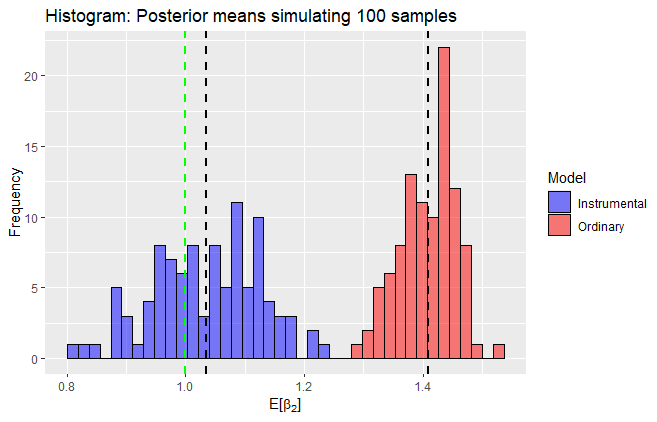
\includegraphics[width=340pt, height=200pt]{Chapters/chapter7/figures/Fig71.png}
	\caption[List of figure caption goes here]{Histogram of posterior means: Ordinary and instrumental models.}\label{fig71}
\end{figure}

Algorithm \ref{alg:IVReg} can be used to estimate the instrumental variable model using our GUI. We ask in Exercise 8 to replicate the example of the effect of institutions on per capita GDP using our GUI.  

\begin{algorithm}[h!]
	\caption{Instrumental variable model}\label{alg:IVReg}
	\begin{algorithmic}[1]  		 			
		\State Select \textit{Multivariate Models} on the top panel
		\State Select \textit{Variable instrumental (two equations)} model using the left radio button
		\State Upload the dataset selecting first if there is header in the file, and the kind of separator in the \textit{csv} file of the dataset (comma, semicolon, or tab). Then, use the \textit{Browse} button under the \textbf{Choose File} legend
		\State Select MCMC iterations, burn-in and thinning parameters using the \textit{Range sliders}
		\State Write down the formula of the structural equation in the \textbf{Main Equation} box. This formula must be written using the syntax of the \textit{formula} command of \textbf{R} software. This equation includes intercept by default, do not include it in the equation
		\State Write down the formula of the endogenous regressor in the \textbf{Instrumental Equation} box. This formula must be written using the syntax of the \textit{formula} command of \textbf{R} software. This equation includes intercept by default, do not include it in the equation
		\State Set the hyperparameters: mean vectors, covariance matrices, degrees of freedom, and the scale matrix. This step is not necessary as by default our GUI uses non-informative priors
		\State Click the \textit{Go!} button
		\State Analyze results
		\State Download posterior chains and diagnostic plots using the \textit{Download Posterior Chains} and \textit{Download Posterior Graphs} buttons
	\end{algorithmic} 
\end{algorithm}

\section{Multivariate probit model}\label{sec74}

In the multivariate probit model \cite{Edwards2003}, the response variable \( y_{il} = \{0, 1\} \) indicates that individual \( i \) makes binary choices among \( L \) mutually exclusive alternatives, where \( l = 1, 2, \dots, L \) and \( i = 1, 2, \dots, N \). Specifically, 
\begin{align*}
	y_{il} = \begin{cases}
		0, & \quad y_{il}^* \leq 0 \\
		1, & \quad y_{il}^* > 0
	\end{cases}
\end{align*}
where \( \bm{y}_i^* = \bm{X}_i \bm{\beta} + \bm{\mu}_i \sim \text{i.i.d.} \, N(\bm{0}, \bm{\Sigma}) \). Here, \( \bm{y}_i^* \) is an unobserved latent \( L \)-dimensional vector, \( \bm{X}_i = \bm{x}_i^\top \otimes \bm{I}_L \) is an \( L \times K \) design matrix of regressors, with \( K = L \times k \), where \( k \) is the number of regressors (i.e., the length of \( \bm{x}_i \)). In addition, \( \bm{\beta} = \left[\bm{\beta}_1^\top \ \bm{\beta}_2^\top \dots \bm{\beta}_k^\top\right]^\top \), where \( \bm{\beta}_j \) forms an \( L \)-dimensional vector of coefficients for \( j = 1, 2, \dots, k \).

The likelihood function for this model is given by 
\[
p(\bm{\beta}, \bm{\Sigma} \mid \bm{y}, \bm{X}) = \prod_{i=1}^N \prod_{l=1}^L p_{il}^{y_{il}},
\]
where \( p_{il} = p(y_{il}^* \geq 0) \).

Observe that $p({y}_{il}^*\geq 0)=p({\lambda}_{ll}{y}_{il}^*\geq 0)$, $\lambda_{ll}>0$. This generates identification issues because just the correlation matrix can be identified, same case as the univariate probit model where the variance of the model is fixed to 1. We follow the post processing strategy proposed by \cite{Edwards2003} to get identified parameters, that is, $\tilde{\bm{\beta}}=vec\left\{\bm{\Lambda}\bm{B}\right\}$ and the correlation matrix $\bm{R}=\bm{\Lambda}\bm{\Sigma}\bm{\Lambda}$, where $\bm{\Lambda}=diag\left\{\sigma_{ll}\right\}^{-1/2}$ and $\bm{B}=\left[\bm{\beta}_1 \ \bm{\beta}_2\dots \bm{\beta}_k\right]$.\footnote{In a Bayesian setting, a model can be non-identified; however, the posterior distribution of the model parameters exists as long as a proper prior distribution is specified \cite{Edwards2003}.}

We assume independent priors: $\bm{\beta} \sim N(\bm{\beta}_0, \bm{B}_0)$ and $\bm{\Sigma}^{-1} \sim W(\alpha_0, \bm{\Psi}_0)$. We can apply Gibbs sampling to this model, as it is a standard Bayesian linear regression model when data augmentation in $\bm{y}^*$ is used.

The posterior conditional distributions are
\begin{equation*}
	\bm{\beta}\mid \bm{\Sigma},\bm{w}\sim{N}(\bm{\beta}_n,\bm{B}_n),
\end{equation*}
\begin{equation*}
	\bm{\Sigma}^{-1}\mid \bm{\beta},\bm{w}\sim{W}(\alpha_n,\bm{\Psi}_n),
\end{equation*}
\begin{equation*}
	y_{il}^*\mid \bm{y}_{i,-l}^*,\bm{\beta},\bm{\Sigma}^{-1},\bm{y_i}\sim{T}{N}_{I_{il}}(m_{il},\tau_{ll}^2)
\end{equation*}

where $\bm{B}_n=(\bm{B}_0^{-1}+\bm{X}^{*\top}\bm{X}^*)^{-1}$, $\bm{\beta}_n=\bm{B}_n(\bm{B}_0^{-1}\bm{\beta}_0+\bm{X}^{*\top}\bm{y}^{**})$, $\bm{\Sigma}^{-1}=\bm{C}^{\top}\bm{C}$, $\bm{X}_i^{*}=\bm{C}^{\top}\bm{X}_i$, $\bm{y}_i^{**}=\bm{C}^{\top}\bm{y}_i^*$, $\alpha_n=\alpha_0+N$, $\bm{\Psi}_n=(\bm{\Psi}_0+\sum_{i=1}^N (\bm{y}_i^*-\bm{X}_i\bm{\beta})(\bm{y}_i^*-\bm{X}_i\bm{\beta})^{\top})^{-1}$,  $m_{il}=\bm{x}_{il}^{\top}\bm{\beta}+\bm{f}_l^{\top}(\bm{y}_{i,-l}^*-\bm{X}_{i,-l}\bm{\beta})$, $\bm{y}_{i,-l}^*$ is an $L-1$ dimensional vector of all components of $\bm{y}_i^*$ excluding $y_{il}^*$, $\bm{x}_{il}^{\top}$ is the $l$-th row of $\bm{X}_i$, $\bm{X}_{i,-l}$ is $\bm{X}_{i}$ after deleting the $l$-th row, $\bm{f}_l^{\top}=\bm{\omega}_{l,-l}^{\top}\bm{\Sigma}_{-l,-l}^{-1}$, $\bm{\omega}_{l,-l}^{\top}$ and $\bm{\Sigma}_{-l,-l}$ are the $l$-th row of $\bm{\Sigma}$ extracting the $l$-th element, and the sub-matrix of $\bm{\Sigma}$ extracting the $l,l$ element, and $\tau_{ll}^2=\sigma_{l,l}-\bm{\omega}_{l,-l}^{\top}\bm{\Sigma}_{-l,-l}^{-1}\bm{\omega}_{-l,l}$, and 
\begin{align*}
	\bm{X}^*=\begin{bmatrix}\bm{X}_1^*\\
		\bm{X}_2^*\\
		\vdots\\
		\bm{X}_N^*
	\end{bmatrix}, & \ I_{il}=\begin{Bmatrix} y_{il}^*> 0, & y_{il}=1\\
	y_{il}^*\leq 0 , & y_{il}=0\\
\end{Bmatrix},\text{ and}&\bm{\Sigma}=\begin{bmatrix}\bm{\omega}_1^{\top} \\ \bm{\omega}_2^{\top} \\ \vdots \\ \bm{\omega}_{L}^{\top} \end{bmatrix}.
\end{align*}

The setting in our GUI has same regressors in each binary decision. However, we can see that the multivariate probit model is similar to a SUR model in latent variables. We ask in Exercise 9 to implement a Gibbs sampling algorithm for a multivariate probit model with different regressors in each equation.\\

\textbf{Example: Self selection in hospitalization due to a subsidized health care program}

We use the dataset \textit{7HealthMed.csv}, where the dependent variable is $y = \left[\text{Hosp} \ \text{SHI}\right]^{\top}$, with $\text{Hosp} = 1$ if an individual was hospitalized in the year prior to the survey (0 otherwise), and $\text{SHI} = 1$ if the individual had subsidized health insurance (0 otherwise).

Recall that our application of binary response models aimed to uncover the determinants of hospitalization in Medellín (Colombia), where one of the regressors was a binary indicator of participation in a subsidized health care program (Section \ref{sec63}). We can use a bivariate probit model if we suspect there is dependence between the decisions regarding these two variables. A priori, we would expect that being in a subsidized health care program increases the probability of hospitalization \textit{ceteris paribus}, due to reduced costs for the patient. However, if an individual expects to be hospitalized in the future, and the factors influencing this decision are unobserved by the modeler, a feedback effect may exist from hospitalization to enrollment in the subsidized health care program.

\begin{algorithm}[h!]
	\caption{Multivariate probit model}\label{alg:MtultProbit}
	\begin{algorithmic}[1]  		 			
		\State Select \textit{Multivariate Models} on the top panel
		\State Select \textit{Multivariate Probit} model using the left radio button
		\State Upload the dataset selecting first if there is header in the file, and the kind of separator in the \textit{csv} file of the dataset (comma, semicolon, or tab). Then, use the \textit{Browse} button under the \textbf{Choose File} legend
		\State Select MCMC iterations, burn-in and thinning parameters using the \textit{Range sliders}
		\State Write down the number of cross-sectional units in the \textbf{Number of individuals: n} box
		\State Write down the number of exogenous variables in the \textbf{Number of exogenous variables: k} box
		\State Write down the number of choices in the \textbf{Number of choices: l} box
		\State Set the hyperparameters: mean vectors, covariance matrix, degrees of freedom, and the scale matrix. This step is not necessary as by default our GUI uses non-informative priors
		\State Click the \textit{Go!} button
		\State Analyze results
		\State Download posterior chains and diagnostic plots using the \textit{Download Posterior Chains} and \textit{Download Posterior Graphs} buttons
	\end{algorithmic} 
\end{algorithm}
We considered seven regressors: a constant, gender (female), age, self-perception of health status (with categories fair, good, and excellent, using bad as the reference category), and the proportion of the individual’s age spent living in their neighborhood. The last variable attempts to account for social capital, which can affect enrollment in the subsidized health insurance program, as the target population is identified by the local government \cite{Ramirez2019a}. The dataset includes 12,975 individuals who can ``choose" two options: hospitalization and enrollment in the subsidized health insurance regime.

Algorithm \ref{alg:MtultProbit} shows how to run a multivariate probit model using our GUI.
\begin{tcolorbox}[enhanced,width=4.67in,center upper,
	fontupper=\large\bfseries,drop shadow southwest,sharp corners]
	\textit{R code. Self selection in hospitalization}
	\begin{VF}
		\begin{lstlisting}[language=R]
rm(list = ls()); set.seed(010101)
Data <- read.csv("https://raw.githubusercontent.com/besmarter/BSTApp/refs/heads/master/DataApp/7HealthMed.csv", sep = ",", header = TRUE, quote = "")
attach(Data); str(Data)
p <- 2; nd <- 7; N <- length(y)/p; y <- y
Xd <- as.matrix(Data[seq(1, p*N, 2),3:9])
XcreateMP<-function(p,nxs,nind,Data){
	pandterm = function(message) {
		stop(message, call. = FALSE)
	}
	if (missing(nxs)) 
	pandterm("requires number of regressors: include intercept if required")
	if (missing(nind)) 
	pandterm("requires number of units (individuals)")
	if (missing(Data)) 
	pandterm("requires dataset")
	if (nrow(Data)!=nind*2)
	pandterm("check dataset! number of units times number alternatives should be equal to dataset rows")
	XXDat<-array(0,c(p,1+nxs,nind))
	XX<-array(0,c(p,nxs*p,nind))
	YY<-array(0,c(p,1,nind))
	is<- seq(p,nind*p,p)
	cis<- seq(nxs,nxs*p+1,nxs)
	for(i in is){
		j<-which(i==is)
		XXDat[,,j]<-as.matrix(Data[c((i-(p-1)):i),-1])
		YY[,,j]<-XXDat[,1,j]
		for(l in 1:p){
			XX[l,((cis[l]-(nxs-1)):cis[l]),j]<-XXDat[l,-1,j]
		}
	}
	return(list(y=YY,X=XX))
}
Dat <- XcreateMP(p = p, nxs = nd, nind = N, Data = Data)
y<-NULL; X<-NULL
for(i in 1:dim(Dat$y)[3]){
	y<-c(y,Dat$y[,,i])
	X<-rbind(X,Dat$X[,,i])
}
DataMP = list(p=p, y=y, X=X)
# Hyperparameters
k <- dim(X)[2]; b0 <- rep(0, k); c0 <- 1000
B0 <- c0*diag(k); B0i <- solve(B0)
a0 <- p - 1 + 3; Psi0 <- a0*diag(p)
Prior <- list(betabar = b0, A = B0i, nu = a0, V = Psi0)
# MCMC parameters
mcmc <- 20000; thin <- 5; 
Mcmc <- list(R = mcmc, keep = thin)
\end{lstlisting}
	\end{VF}
\end{tcolorbox}

\begin{tcolorbox}[enhanced,width=4.67in,center upper,
	fontupper=\large\bfseries,drop shadow southwest,sharp corners]
	\textit{R code. Self selection in hospitalization, results}
	\begin{VF}
		\begin{lstlisting}[language=R]
Results <- bayesm::rmvpGibbs(Data = DataMP, Mcmc = Mcmc, Prior = Prior)
betatilde1 <- Results$betadraw[,1:7] / sqrt(Results$sigmadraw[,1])
summary(coda::mcmc(betatilde1))
Quantiles for each variable:

				2.5%       25%       50%       75%     97.5%
var1 -1.2247602 -1.059257 -0.970870 -0.889741 -0.733411
var2  0.0269885  0.090098  0.121863  0.155585  0.220662
var3  0.0007652  0.002207  0.002925  0.003685  0.005049
var4 -0.7477149 -0.598898 -0.522549 -0.445173 -0.296718
var5 -1.4520842 -1.309922 -1.234633 -1.160468 -1.018396
var6 -1.3503717 -1.182381 -1.092511 -1.005472 -0.837939
var7 -0.1791758 -0.103506 -0.064418 -0.024499  0.051849
betatilde2 <- Results$betadraw[,8:14] / sqrt(Results$sigmadraw[,4])
summary(coda::mcmc(betatilde2))
Quantiles for each variable:
				2.5%       25%       50%       75%    97.5%
var1  0.306343  0.477265  0.564698  0.656616  0.82932
var2  0.258347  0.289819  0.305902  0.322116  0.35284
var3  0.007848  0.008656  0.009124  0.009591  0.01045
var4 -0.488810 -0.313532 -0.218459 -0.130373  0.04144
var5 -0.677686 -0.511529 -0.418139 -0.332415 -0.17322
var6 -0.703355 -0.527642 -0.433378 -0.341355 -0.16989
var7  0.164388  0.203623  0.224533  0.245306  0.28513
sigmadraw12 <-  Results$sigmadraw[,3] / (Results$sigmadraw[,1]*Results$sigmadraw[,4])^0.5
summary(coda::mcmc(sigmadraw12))
Quantiles for each variable:
2.5%       25%       50%       75%     97.5% 
-0.070515 -0.025009 -0.002895  0.018432  0.060986
\end{lstlisting}
	\end{VF}
\end{tcolorbox}

We set 20,000 MCMC iterations with a thinning parameter equal to 5. The hyperparameters are $\bm{\beta}_0 = \bm{0}_{14}$, $\bm{B}_0 = 100\bm{I}_{14}$, $\alpha_0 = 4$, and $\bm{\Psi}_0 = 4\bm{I}_2$.\footnote{Note that the order of the location coefficients in our GUI follows the equations, not the order of the regressors as in the theoretical setting presented in this section. This distinction is important for correctly setting the hyperparameters and interpreting the results of the location parameters.}

The previous \textbf{R} code demonstrates how to obtain the posterior draws using the \textit{rmvpGibbs} command from the \textit{bayesm} package. The results suggest that females, older individuals, and those who self-assess their health as poor are more likely to be hospitalized. Furthermore, females, older individuals, and those with a poor or fair self-perception of health, who have lived a larger proportion of their life in their current neighborhood, are more likely to be enrolled in the subsidized health care system. However, the results indicate that there is no unobserved correlation between the two equations, as the 95\% credible interval for the correlation is (-0.07, 0.06).

\section{Summary}\label{sec75}
In this chapter, we present the setting and posterior distributions of the most common multivariate models. The multivariate framework allows us to address \textit{endogeneity} issues by using the conditional distribution of a multivariate normal vector. Moreover, we always obtain posterior conditional distributions that belong to standard families (multivariate normal, Wishart, and truncated normal) in these models. This property enables the implementation of the Gibbs sampling algorithm for all these models.

\section{Exercises}\label{sec76}
\begin{enumerate}
	\item Show that $\mathbb{E}[u_1\text{PAER}] = \frac{\alpha_1}{1 - \beta_1\alpha_1} \sigma_1^2$, assuming that $\mathbb{E}[u_1 u_2] = 0$, where $\text{Var}(u_1) = \sigma_1^2$, in the example of the effect of institutions on per capita GDP.
	
	\item Show that $\beta_1=\pi_1/\gamma_1$, in the example of the effect of institutions on per capita GDP.
	
	\item \textbf{The effect of institutions on per capita gross domestic product continues I}
	
	Use the \textit{rmultireg} command from the \textit{bayesm} package to perform inference in the example of the effect of institutions on per capita GDP. 
	
	\item \textbf{Demand and supply simulation}
	
	Given the structural demand-supply model:
\begin{align*}
	q_i^d &= \beta_1 + \beta_2 p_i + \beta_3 y_i + \beta_4 pc_i + \beta_5 ps_i + u_{i1}, \\
	q_i^s &= \alpha_1 + \alpha_2 p_i + \alpha_3 er_i + u_{i2},
\end{align*}
where $q^d$ is demand, $q^s$ is supply, $p$, $y$, $pc$, $ps$, and $er$ are price, income, complementary price, substitute price, and exchange rate, respectively. Complementary and substitute prices refer to the prices of complementary and substitute goods for $q$. Assume that $\bm{\beta} = \left[ 5 \ -0.5 \ 0.8 \ -0.4 \ 0.7 \right]^{\top}$, $\bm{\alpha} = \left[ -2 \ 0.5 \ -0.4 \right]^{\top}$, $u_1 \sim N(0, 0.5^2)$, and $u_2 \sim N(0, 0.5^2)$. Additionally, assume that $y \sim N(10, 1)$, $pc \sim N(5, 1)$, $ps \sim N(5, 1)$, and $er \sim N(15, 1)$.

\begin{itemize}
	\item Find the \textit{reduced-form} model by using the condition that in equilibrium, demand and supply are equal, i.e., $q^d = q^s$. This condition defines the observable quantity, $q$.
	\item Simulate $p$ and $q$ from the \textit{reduced-form} equations.
	\item Perform inference for the \textit{reduced-form} model using the \textit{rmultireg} command from the \textit{bayesm} package.
	\item Use the posterior draws of the \textit{reduced-form} parameters to perform inference for the \textit{structural} parameters. Any issues? Hint: Are all \textit{structural} parameters exactly identified?
\end{itemize}

\item \textbf{Utility demand continues}

\begin{itemize}
	\item Run the \textbf{Utility demand} application using our GUI and the information in the dataset \textit{Utilities.csv}. Hint: This file should be modified to agree the structure that requires our GUI (see the dataset \textit{5Institutions.csv} in the folder \textit{DataApp} of our GitHub repository -\textbf{https://github.com/besmarter/BSTApp}- for a template).
	\item Program from scratch the Gibbs sampler algorithm in this application.   
\end{itemize}

\item \textbf{Simulation exercise of instrumental variables continues I}

\begin{itemize}
	\item Use the setting of the simulation exercise with instrumental variables to analyze the impact of a weak instrument. For instance, set $\gamma_2 = 0.2$ and compare the performance of the posterior means of the ordinary and instrumental variable models.
	\item Perform a simulation to analyze how the degree of exogeneity of the instrument affects the performance of the posterior mean in the instrumental variable model.
\end{itemize}

\item \textbf{Simulation exercise of instrumental variables continues II}

Program from scratch the Gibbs sampling algorithm of the instrumental model for the simulation exercise of the instrumental variables.

\item \textbf{The effect of institutions on per capita gross domestic product continues II}

Estimate the structural Equation \ref{eq:str1} using the instrumental variable model where the instrument of PAER is $\log(\textit{Mort})$. Compare the effect of property rights on per capita GDP of this model with the effect estimated in the example of the effect of institutions on per capita gross domestic product. Use the file \textit{6Institutions.csv} to do this exercise in our GUI, and set $\bm{B}_0=100\bm{I}_5$, $\bm{\beta}_0=\bm{0}_5$, $\bm{\gamma}_0=\bm{0}_2$, $\bm{G}_0=100\bm{I}_2$ $\alpha_0=3$ and $\bm{\Psi}_0=3\bm{I}_2$. The MCMC iterations, burn-in and thinning parameters are 50000, 1000 and 5, respectively.

\item \textbf{Multivariate probit with different regressors}

Let's do a simulation exercise where $y_{i1}^*=0.5-1.2x_{i11}+0.7x_{i12}+0.8x_{i3}+\mu_{i1}$ and $y_{i2}^*=1.5-0.8x_{i21}+0.5x_{i22}+\mu_{i2}$, $\bm{\Sigma}=\begin{bmatrix}
	1 & 0.5\\
	0.5 & 1
\end{bmatrix}$, where all regressors distribute standard normal, and $N=5000$. Use $\bm{\beta}_0=\bm{0}$, $\bm{B}_0=1000\bm{B}$, $\alpha_0=4$ and $\bm{\Psi}_0=4\bm{I}_2$. Set number of iterations 2000 and a thinning parameter equal to 5.  

\begin{itemize}
	\item Perform inference using the setting of Section \ref{sec74}, that is, assuming that $x_{i3}$ could have an effect on $y_{i2}$.
	\item Program a Gibss sampling algorithm taking into account that there are different regressors in each binary decision, that is, $x_{i3}$ does not have an effect on $y_{i2}$. 
\end{itemize}      

\end{enumerate}



\chapter{Time series models}\label{chap8}
In this chapter, we provide a brief introduction to performing inference in time series models using a Bayesian framework. There is a large literature in time series in statistics and econometrics, and it would be impossible to present a good treatment in a few pages of an introductory book. However, there are excellent books in Bayesian inference in time series, see for instance, \cite{west2006bayesian,petris2009dynamic,pole2018applied}.

A time series is a sequence of observations collected in chronological order, allowing us to track how variables change over time. However, it also introduces technical challenges, as we must account for statistical features such as autocorrelation and stationarity. Since time series data is time-dependent, we adjust our notation. Specifically, we use $t$ and $T$ instead of $i$ and $N$ to explicitly indicate time.

Our starting point in this chapter is the \textit{state-space representation} of time series models. Much of the Bayesian inference literature in time series adopts this approach, as it allows dynamic systems to be modeled in a structured way. This representation provides modularity, flexibility, efficiency, and interpretability in complex models where the state evolves over time. It also enables the use of recursive estimation methods, such as the \textit{Kalman filter} for dynamic Gaussian linear models and the \textit{particle filter} (also known as \textit{sequential Monte Carlo}) for non-Gaussian and nonlinear state-space models. The latter method is especially useful for \textit{online} predictions or when there are data storage limitations. These inferential tools are based on the sequential updating process of Bayes' rule, where the posterior at time $t$ becomes the prior at time $t+1$ (see Equation \ref{equpdate}).

Remember that we can run our GUI typing

\begin{tcolorbox}[enhanced,width=4.67in,center upper,
	fontupper=\large\bfseries,drop shadow southwest,sharp corners]
	\textit{R code. How to display our graphical user interface}
	\begin{VF}
		\begin{lstlisting}[language=R]
		shiny::runGitHub("besmarter/BSTApp", launch.browser = T)\end{lstlisting}
	\end{VF}
\end{tcolorbox} 

in the \textbf{R} package console or any \textbf{R} code editor, and once our GUI is deployed, select \textit{Time series Models}. However, users should see Chapter \ref{chapGUI} for details.

\section{State-space representation}\label{sec81}
A \textit{state-space model} is composed by of an \textit{unobservable state vector}  $\bm{\beta}_t \in \mathbb{R}^K$, and an \textit{observed} measure $\bm{Y}_t \in \mathbb{R}^M$, $t=1,2,\dots$ such that (i) $\bm{\beta}_t$ is a \textit{Markov process}, this is, $\pi(\bm{\beta}_t|\bm{\beta}_{1:t-1})=\pi(\bm{\beta}_t|\bm{\beta}_{t-1})$, all the information regarding $\bm{\beta}_t$ based on all its history up to $t-1$ is carried by $\bm{\beta}_{t-1}$, and (ii) $\bm{Y}_t$ is independent of $\bm{Y}_s$ conditional on $\bm{\beta}_t$, $t\neq s$ \cite[Chap.~2]{petris2009dynamic}.

These assumptions imply that $\pi(\bm{\beta}_{0:t},\bm{Y}_{1:t})=\pi(\bm{\beta}_0)\prod_{s=1}^{t}\pi(\bm{\beta}_s|\bm{\beta}_{s-1})\pi(\bm{Y}_s|\bm{\beta}_s)$.\footnote{A \textit{state-space model} where the states are random variables taking discrete values is called \textit{hidden Markov model}.}

There are three key aspects of \textit{state-space models}: \textit{filtering}, \textit{smoothing}, and \textit{forecasting}. In \textit{filtering}, we aim to estimate the current state given observations up to time $t$, specifically obtaining the density $\pi(\bm{\beta}_{s}|\bm{y}_{1:t})$ for $s = t$. In \textit{smoothing}, we conduct a retrospective analysis of the system, obtaining $\pi(\bm{\beta}_{s}|\bm{y}_{1:t})$ for $s < t$. In \textit{forecasting}, we forecast future observations by first obtaining $\pi(\bm{\beta}_{s}|\bm{y}_{1:t})$ as an intermediate step to compute $\pi(\bm{Y}_{s}|\bm{y}_{1:t})$ for $s > t$. A valuable feature of these methods is that all these densities can be calculated recursively. \cite{petris2009dynamic} show the recursive equations in Propositions 2.1 (filtering), 2.3 (smoothing) and 2.5 (forecasting).

An important class of \textit{state-space models} is the \textit{Gaussian linear state-space model}, also know as, \textit{dynamic linear model}:
\begin{align*}
	\bm{Y}_t&=\bm{X}_t\bm{\beta}_t+\bm{\mu}_t& \text{(Observation equations)}\\
	\bm{\beta}_t&=\bm{G}_t\bm{\beta}_{t-1}+\bm{w}_t & \text{(States equations)},
\end{align*}
where $\bm{\beta}_0\sim N(\bm{b}_0,\bm{B}_0)$, $\bm{\mu}_t\sim N(\bm{0}, \bm{\Sigma}_t)$, $\bm{w}_t\sim N(\bm{0}, \bm{\Omega}_t)$, $\bm{\beta}_0$, $\bm{\mu}_t$ and $\bm{w}_t$ are independent, $\bm{X}_t$ and $\bm{G}_t$ are $M\times K$ and $K\times K$ known matrices. Observe that this assumptions implies that $\bm{Y}_t|\bm{\beta}_t\sim N(\bm{X}_t\bm{\beta}_t,\bm{\Sigma}_t)$, and $\bm{\beta}_t|\bm{\beta}_{t-1}\sim N(\bm{G}_t\bm{\beta}_{t-1},\bm{\Omega}_t)$.\footnote{A general \textit{state-space model} is given by $\bm{Y}_t=\bm{f}_t(\bm{\beta}_t,\bm{\mu}_t)$, and $\bm{\beta}_t=\bm{m}_t(\bm{\beta}_{t-1},\bm{w}_t)$ for arbitrary functions $\bm{f}_t$ and $\bm{m}_t$, and distributions for $\bm{\mu}_t$ and $\bm{w}_t$, and a prior distribution for $\bm{\beta}_0$.}

Let $\bm{\beta}_{t-1}|\bm{y}_{1:t-1}\sim N(\bm{b}_{t-1},\bm{B}_{t-1})$, then, we can get the \textit{Kalman filter} by getting
\begin{enumerate}
	\item The one-step-ahead predictive distribution of $\bm{\beta}_t$ given $\bm{y}_{1:t-1}$ is $\bm{\beta}_t|\bm{y}_{1:t-1}\sim N(\bm{a}_t, \bm{R}_t)$, where $\bm{a}_t=\bm{G}_t\bm{b}_{t-1}$ and $\bm{R}_t=\bm{G}_t\bm{B}_{t-1}\bm{G}_t^{\top}+\bm{\Omega}_t$.
	\item  The one-step-ahead predictive distribution of $\bm{Y}_t$ given $\bm{y}_{1:t-1}$ is $\bm{Y}_t|\bm{y}_{1:t-1}\sim N(\bm{f}_t, \bm{Q}_t)$, where $\bm{f}_t=\bm{X}_t\bm{a}_t$ and $\bm{Q}_t=\bm{X}_t\bm{R}_t\bm{X}_t^{\top}+\bm{\Sigma}_t$.
	\item The distribution of the one-step-ahead prediction error  $\bm{e}_t=\bm{Y}_t-\mathbb{E}[\bm{Y}_t|\bm{y}_{1:t-1}]=\bm{Y}_t-\bm{f}_t$ is $N(\bm{0}, \bm{Q}_t)$ \cite[Chap.~6]{shumway2017time}. 
	\item The filtering distribution of $\bm{\beta}_t$ given $\bm{y}_{1:t}$ is $\bm{\beta}_t|\bm{y}_{1:t}\sim N(\bm{b}_t, \bm{B}_t)$, where $\bm{b}_t=\bm{a}_t+\bm{K}_t\bm{e}_t$, $\bm{K}_t=\bm{R}_t\bm{X}_t^{\top}\bm{Q}_t^{-1}$ is the \textit{Kalman gain}, and $\bm{B}_t=\bm{R}_t-\bm{R}_t\bm{X}_t^{\top}\bm{Q}_t^{-1}\bm{X}_t\bm{R}_t$.   
\end{enumerate}    

The formal proofs of these results can be found in \cite[Chap~2]{petris2009dynamic}. Just take into account that the logic of these results follow the results of the Seemingly unrelated regression (SUR) model in Section \ref{sec72} for a particular time period. In addition, we know that the posterior distribution using information up to $t-1$ becomes the prior in $t$ (see Equation \ref{equpdate}, $\pi(\bm{\theta}|\mathbf{y}_{1:t})\propto p(y_{t}|\bm{y}_{1:t-1},\bm{\theta})\times \pi(\bm{\theta}|\bm{y}_{1:t-1})$). This is the updating process from  $\bm{\beta}_t|\bm{y}_{1:t-1}\sim N(\bm{a}_t, \bm{R}_t)$ to $\bm{\beta}_t|\bm{y}_{1:t}\sim N(\bm{b}_t, \bm{B}_t)$. Moreover, the posterior mean and variance of the SUR model with independent conjugate priors for a particular time period can be written as $\bm{a}_{t}+\bm{R}_{t}\bm{X}_t^{\top}(\bm{X}_t\bm{R}_{t}\bm{X}_t^{\top}+ \bm{\Sigma}_t)^{-1}(\bm{y}_t-\bm{X}_t\bm{a}_{t})$ and $\bm{R}_{t}-\bm{R}_{t}\bm{X}_t^{\top}(\bm{X}_t\bm{R}_{t}\bm{X}_t^{\top}+\bm{\Sigma}_t)^{-1} \bm{X}_t\bm{R}_{t}^{\top}$, respectively. Let's see this, we know from Section \ref{sec72} that $\bm{B}_t=(\bm{R}_t^{-1}+\bm{X}_t^{\top}\bm{\Sigma}^{-1}\bm{X}_t)^{-1}$ and $\bm{\beta}_t=\bm{B}_t(\bm{R}_t^{-1}\bm{a}_t+\bm{X}_t^{\top}\bm{\Sigma}^{-1}\bm{y}_t)$. Thus, let's show that both conditional posterior distributions are the same. In particular, the posterior mean in the \textit{state-space representation} is $[\bm{I}_K-\bm{R}_{t}\bm{X}_t^{\top}(\bm{X}_t\bm{R}_{t}\bm{X}_t^{\top}+ \bm{\Sigma}_t)^{-1}\bm{X}_t]\bm{a}_{t}+\bm{R}_{t}\bm{X}_t^{\top}(\bm{X}_t\bm{R}_{t}\bm{X}_t^{\top}+ \bm{\Sigma}_t)^{-1}\bm{y}_t$, where 
\begin{align*}
	\bm{R}_{t}\bm{X}_t^{\top}(\bm{X}_t\bm{R}_{t}\bm{X}_t^{\top}+ \bm{\Sigma}_t)^{-1}
	&=\bm{R}_{t}\bm{X}_t^{\top}[\bm{\Sigma}_t^{-1}-\bm{\Sigma}_t^{-1}\bm{X}_t(\bm{R}_t^{-1}+\bm{X}_t^{\top}\bm{\Sigma}_t^{-1}\bm{X}_t)^{-1}\bm{X}_t^{\top}\bm{\Sigma}_t^{-1}]\\
	&=\bm{R}_{t}[\bm{I}_K-\bm{X}_t^{\top}\bm{\Sigma}_t^{-1}\bm{X}_t(\bm{R}_t^{-1}+\bm{X}_t^{\top}\bm{\Sigma}_t^{-1}\bm{X}_t)^{-1}]\bm{X}_t^{\top}\bm{\Sigma}_t^{-1}\\
	&=\bm{R}_{t}(\bm{I}_K-[\bm{I}_K-\bm{R}_t^{-1}(\bm{R}_t^{-1}+\bm{X}_t^{\top}\bm{\Sigma}_t^{-1}\bm{X}_t)^{-1}])\bm{X}_t^{\top}\bm{\Sigma}_t^{-1}\\
	&=(\bm{R}_t^{-1}+\bm{X}_t^{\top}\bm{\Sigma}_t^{-1}\bm{X}_t)^{-1}\bm{X}_t^{\top}\bm{\Sigma}_t^{-1},
\end{align*}
where the first equality uses the Woodbury matrix identity (matrix inversion lemma), and the third equality uses $\bm{D}(\bm{D}+\bm{E})^{-1}=\bm{I}-\bm{E}(\bm{D}+\bm{E})^{-1}$. 

Thus, $[\bm{I}_K-\bm{R}_{t}\bm{X}_t^{\top}(\bm{X}_t\bm{R}_{t}\bm{X}_t^{\top}+ \bm{\Sigma}_t)^{-1}\bm{X}_t]\bm{a}_{t}+\bm{R}_{t}\bm{X}_t^{\top}(\bm{X}_t\bm{R}_{t}\bm{X}_t^{\top}+ \bm{\Sigma}_t)^{-1}\bm{y}_t=[\bm{I}_K-(\bm{R}_t^{-1}+\bm{X}_t^{\top}\bm{\Sigma}_t^{-1}\bm{X}_t)^{-1}\bm{X}_t^{\top}\bm{\Sigma}_t^{-1}\bm{X}_t]\bm{a}_{t}+(\bm{R}_t^{-1}+\bm{X}_t^{\top}\bm{\Sigma}_t^{-1}\bm{X}_t)^{-1}\bm{X}_t^{\top}\bm{\Sigma}_t^{-1}\bm{y}_t=(\bm{R}_t^{-1}+\bm{X}_t^{\top}\bm{\Sigma}_t^{-1}\bm{X}_t)^{-1}\bm{R}_t^{-1}\bm{a}_{t}+(\bm{R}_t^{-1}+\bm{X}_t^{\top}\bm{\Sigma}_t^{-1}\bm{X}_t)^{-1}\bm{X}_t^{\top}\bm{\Sigma}_t^{-1}\bm{y}_t=(\bm{R}_t^{-1}+\bm{X}_t^{\top}\bm{\Sigma}_t^{-1}\bm{X}_t)^{-1}(\bm{R}_t^{-1}\bm{a}_{t}+\bm{X}_t^{\top}\bm{\Sigma}_t^{-1}\bm{y}_t)=(\bm{R}_t^{-1}+\bm{X}_t^{\top}\bm{\Sigma}_t^{-1}\bm{X}_t)^{-1}(\bm{R}_t^{-1}\bm{a}_{t}+\bm{X}_t^{\top}\bm{\Sigma}_t^{-1}\bm{X}_t\hat{\bm{\beta}}_t)$. The second equality uses $\bm{I}-(\bm{D}+\bm{E})^{-1}\bm{D}=(\bm{D}+\bm{E})^{-1}\bm{E}$, and $\hat{\bm{\beta}}_t=(\bm{X}_t^{\top}\bm{\Sigma}_t^{-1}\bm{X}_t)^{-1}\bm{X}_t^{\top}\bm{\Sigma}_t^{-1}\bm{y}_t$. This means that the posterior mean is a weighted average of the prior mean, and the maximum likelihood estimator (generalized least squares estimator).

The weights are linked to the signal-to-noise ratio, that is, the proportion of the total variability ($\bm{\Omega}_t+\bm{\Sigma}_t$) due to the signal ($\bm{\Omega}_t$) versus the noise ($\bm{\Sigma}_t$). Note that in the simplest case where $M=K=1$, and $\bm{X}_t=\bm{G}_t=1$, then $\bm{K}_t=\bm{R}_t\bm{Q}_t^{-1}=(B_{t-1}+\Omega_t)/(B_{t-1}+\Omega_t+\Sigma_t)$. Thus, the weight associated with the observations is equal to 1 if $\Sigma_t=0$, that is, the posterior mean is equal to the actual observation. On the other hand, if $\Sigma_t$ increases compare to $\Omega_t$, there is more weight to the prior information, and consequently, the posterior mean is smoother as it heavily dependents on the history. We ask in Exercise 1 to perform simulations with different signal-to-noise ratios to see the effects on the system.   

The equality of variances of both approaches is as follows:
\begin{align*}
	Var[\bm{\beta}_t|\bm{y}_{1:t}]&
	= \bm{R}_{t}-\bm{R}_{t}\bm{X}_t^{\top}(\bm{X}_t\bm{R}_{t}\bm{X}_t^\top+\bm{\Sigma}_t)^{-1} \bm{X}_t\bm{R}_{t}\\
	&=\bm{R}_{t}-\bm{R}_{t}\bm{X}_t^{\top}(\bm{\Sigma}_t^{-1}- \bm{\Sigma}_t^{-1}\bm{X}_t(\bm{R}_{t}^{-1}+\bm{X}_t^{\top}\bm{\Sigma}_t^{-1}\bm{X}_t)^{-1}\bm{X}_t^{\top}\bm{\Sigma}_t^{-1})\bm{X}_t\bm{R}_{t}\\
	&=\bm{R}_{t}-\bm{R}_{t}\bm{X}_t^{\top}\bm{\Sigma}_t^{-1}\bm{X}_t\bm{R}_{t}+ \bm{R}_{t}\bm{X}_t^{\top}\bm{\Sigma}_t^{-1}\bm{X}_t(\bm{R}_{t}^{-1}+\bm{X}_t^{\top}\bm{\Sigma}_t^{-1}\bm{X}_t)^{-1}\bm{X}_t^{\top}\bm{\Sigma}_t^{-1}\bm{X}_t\bm{R}_{t}\\
	&=\bm{R}_{t}-\bm{R}_{t}\bm{X}_t^{\top}\bm{\Sigma}_t^{-1}\bm{X}_t\bm{R}_{t}+ \bm{R}_{t}\bm{X}_t^{\top}\bm{\Sigma}_t^{-1}\bm{X}_t[\bm{I}_K-(\bm{R}_{t}^{-1}+\bm{X}_t^{\top}\bm{\Sigma}_t^{-1}\bm{X}_t)^{-1}\bm{R}_{t}^{-1}]\bm{R}_{t}\\
	&=\bm{R}_{t}-\bm{R}_{t}\bm{X}_t^{\top}\bm{\Sigma}_t^{-1}\bm{X}_t(\bm{R}_{t}^{-1}+\bm{X}_t^{\top}\bm{\Sigma}_t^{-1}\bm{X}_t)^{-1}\\
	&=\bm{R}_t[\bm{I}_K-\bm{X}_t^{\top}\bm{\Sigma}_t^{-1}\bm{X}_t(\bm{R}_{t}^{-1}+\bm{X}_t^{\top}\bm{\Sigma}_t^{-1}\bm{X}_t)^{-1}]\\
	&=\bm{R}_{t}[\bm{I}_K-(\bm{I}_K-\bm{R}_{t}^{-1}(\bm{R}_{t}^{-1}+\bm{X}_t^{\top}\bm{\Sigma}_t^{-1}\bm{X}_t)^{-1})]\\
	&=(\bm{R}_{t}^{-1}+\bm{X}_t^{\top}\bm{\Sigma}_t^{-1}\bm{X}_t)^{-1},
\end{align*}
where the second equality uses the Woodbury matrix identity, the fourth equality uses $(\bm{D}+\bm{E})^{-1}\bm{D}=\bm{I}-(\bm{D}+\bm{E})^{-1}\bm{E}$, and the seventh equality uses $\bm{D}(\bm{D}+\bm{E})^{-1}=\bm{I}-\bm{E}(\bm{D}+\bm{E})^{-1}$.  

The \textit{Kalman filter} allows calculating recursively in a forward way $\pi(\bm{\beta}_t|\bm{y}_{1:t})$ from $\pi(\bm{\beta}_{t-1}|\bm{y}_{1:t-1})$ starting from $\pi(\bm{\beta}_0)$.

Let $\bm{\beta}_{t+1}|\bm{y}_{1:T}\sim N(\bm{s}_{t+1},\bm{S}_{t+1})$, then we can get the \textit{Kalman smoother} by $\bm{\beta}_{t}|\bm{y}_{1:T}\sim N(\bm{s}_{t},\bm{S}_{t})$, where $\bm{s}_t=\bm{b}_t+\bm{B}_t\bm{G}_{t+1}^{\top}\bm{R}_{t+1}^{-1}(\bm{s}_{t+1}-\bm{a}_{t+1})$ and $\bm{S}_t=\bm{B}_t-\bm{B}_t\bm{G}_{t+1}^{\top}\bm{R}_{t+1}^{-1}(\bm{R}_{t+1}-\bm{S}_{t+1})\bm{R}_{t+1}^{-1}\bm{G}_{t+1}\bm{B}_{t}$. The proof can be found in \cite[Chap~2]{petris2009dynamic}. 

Thus, we can calculate the \textit{Kalman smoother} starting from $t=T-1$, that is, $\bm{\beta}_{T}|\bm{y}_{1:T}\sim N(\bm{s}_{T},\bm{S}_{T})$. However, this is the filtering distribution at $T$, which means $\bm{s}_{T}=\bm{b}_{T}$ and $\bm{S}_{T}=\bm{B}_{T}$, and then, we should proceed recursively in a backward way.

Finally, the forecasting recursion in the \textit{dynamic linear model}, given $\bm{a}_t(0)=\bm{b}_t$ and $\bm{R}_t(0)=\bm{B}_t$, $h\geq 1$, is given by 
\begin{enumerate}
	\item The forecasting distribution of $\bm{\beta}_{t+h}|\bm{y}_{1:t}$ is $N(\bm{a}_t(h),\bm{R}_t(h))$, where $\bm{a}_t(h)=\bm{G}_{t+h}\bm{a}_{t}(h-1)$ and $\bm{R}_t(h)=\bm{G}_{t+h}\bm{R}_t(h-1)\bm{G}_{t+h}^{\top}+\bm{\Omega}_{t+h}$.
	\item The forecasting distribution $\bm{Y}_{t+h}|\bm{y}_{1:t}$ is $N(\bm{f}_t(h),\bm{Q}_t(h))$, where $\bm{f}_t(h)=\bm{X}_{t+h}\bm{a}_t(h)$ and $\bm{Q}_t(h)=\bm{X}_{t+h}\bm{R}_t(h)\bm{X}_{t+h}^{\top}+\bm{\Sigma}_{t+h}$.  
\end{enumerate}
The proof can be found in \cite[Chap~2]{petris2009dynamic}.

These recursive equations allows to perform probabilistic forecasting $h$-steps-ahead for the state and observation equations.

These results show how to use these recursive equations to perform filtering, smoothing and forecasting in \textit{dynamic linear models} (\textit{Gaussian linear state-space models}). Despite that these algorithms look simple, they suffer from numerical instability that lead to non-symmetric and negative definite calculated covariance matrices. Thus, special care should be put when working with them.

In addition, this set up assumes that the $\bm{\Sigma}_t$ and $\bm{\Omega}_t$ are known. However, this is no the case in most situations. Thus, we should estimate them. One option is to perform maximum likelihood estimation. However, this approach does not take into account the uncertainty associated with the fact that $\bm{\Sigma}_t$ and $\bm{\Omega}_t$ are unknown when their estimates are \textit{plug in} the \textit{state space} recursions. On the other hand, we can use a Bayesian approach, and perform the recursions associated with each posterior draw of the unknown parameters. Thus, we take into account their uncertainty.

The point of departure is the posterior distribution, such that
\begin{align*}
	\pi(\bm{\theta},\bm{\beta}_0,\dots,\bm{\beta}_T|\bm{y}, \bm{X}, \bm{G})&\propto\pi(\bm{\beta}_0|\bm{\theta})\pi(\bm{\theta})\prod_{t=1}^{T}\pi(\bm{\beta}_t|\bm{\beta}_{t-1},\bm{\theta})\pi(\bm{y}_t|\bm{\beta}_t,\bm{\theta}),
\end{align*} 
where $\bm{\theta}$ is the vector of unknown parameters.

We can compute $\pi(\bm{\beta}_s,\bm{\theta}|\bm{y}_{1:t})=\pi(\bm{\beta}_s|\bm{y}_{1:t},\bm{\theta})\pi(\bm{\theta}|\bm{y}_{1:t})$, for $s=t$ (\textit{filtering}), $s<t$ (\textit{smoothing}), and $s>t$ (\textit{forecasting}). The marginal posterior distribution of the states is $\pi(\bm{\beta}_s|\bm{y}_{1:t})=\int_{\bm{\Theta}}\pi(\bm{\beta}_s|\bm{y}_{1:t},\bm{\theta})\pi(\bm{\theta}|\bm{y}_{1:t})d\bm{\theta}$.

We can use the Gibbs sampling algorithm to get the posterior draws in the \textit{dynamic linear model} assuming conjugate families. In particular, let's see the univariate case with \textit{random walk states}, 
\begin{align}
	Y_t&=\bm{x}_t^{\top}\bm{\beta}_t+\mu_t\label{eq1Obs}\\
	\bm{\beta}_t&=\bm{\beta}_{t-1}+\bm{w}_t \label{eq1St},
\end{align}
where $\mu_t\sim N(0,\sigma^2)$ and $\bm{w}_t\sim N(\bm{0},\text{diag}\left\{\omega_1^2,\dots,\omega_K^2\right\})$. We assume that $\pi(\sigma^2,\omega_1^2,\dots,\omega_K^2,\bm{\beta}_0)=\pi(\sigma^2)\pi(\omega_1^2),\dots,\pi(\omega_K^2)\pi(\bm{\beta}_0)$ where $\sigma^2\sim IG(\alpha_0/2,\delta_0/2)$, $\omega_k^2\sim IG(\alpha_{k0}/2,\delta_{k0}/2)$, $k=1,\dots,K$, and $\bm{\beta}_0\sim N(\bm{b}_0,\bm{B}_0)$. Thus, the conditional posterior distributions are $\sigma^2|\bm{y},\bm{X},\bm{\beta}_{1:T}\sim IG(\alpha_{n}/2,\delta_n/2)$, where $\alpha_{n}=T+\alpha_0$ and $\delta_n=\sum_{t=1}^T(y_t-\bm{x}_t^{\top}\bm{\beta}_t)^2+\delta_0$, and $\omega_k^2|\bm{y},\bm{X},\bm{\beta}_{0:T}\sim IG(\alpha_{kn}/2,\delta_{kn}/2)$, where $\alpha_{kn}=T+\alpha_{k0}$ and $\delta_{kn}=\sum_{t=1}^T(\bm{\beta}_{t,k}-\bm{\beta}_{t-1,k})^2+\delta_{k0}$. The vector of the dependent variable is $\bm{y}$, and all regressors are in $\bm{X}$.

We also need to sample the states from $\pi(\bm{\beta}_{1:T}|\bm{y},\bm{X},\sigma^2,\omega_1^2,\dots,\omega_K^2)$. This can be done using the forward filtering backward sampling (FFBS) algorithm \cite{carter1994gibbs,fruhwirth1994data,shephard1994partial}. This algorithm is basically a simulation version of the \textit{smoothing} recursion, which allows getting draws of the states, even if we do not have analytical solutions, for instance, in non-linear settings. See below and \cite[Chap.~3]{petris2009dynamic} for details. A word of caution here, users should be careful to set non-informative priors in this setting, and in general, settings where there are a large number of parameters (see \cite[Chap.~8]{koop2003bayesian} for details). Thus, it is useful to use empirical Bayes methods focusing on relevant hyperparameters, for instance, the hyperparameters of the inverse-gamma distributions which define the signal-to-noise ratio.   

We use the command \textit{dlmGibbsDIG} from the \textit{dlm} package in our GUI to perform Bayesian inference in the univariate \textit{dynamic linear model} with \textit{random walk states}. This function uses the FFBS algorithm, and assumes independent inverse-gamma priors for the scale parameters. In addition, this package uses the singular value decomposition to calculate the covariance matrices to avoid numerical instability.

Algorithm \ref{alg:DLM} shows how to perform inference in univariate \textit{dynamic linear model} with random walk states in our GUI. See also Chapter \ref{chapGUI} for details regarding the dataset structure.

\begin{algorithm}[h!]
	\caption{Dynamic linear models}\label{alg:DLM}
	\begin{algorithmic}[1]  		 			
		\State Select \textit{Time series Model} on the top panel
		\State Select \textit{Dynamic linear model} using the left radio button
		\State Upload the dataset selecting first if there is header in the file, and the kind of separator in the \textit{csv} file of the dataset (comma, semicolon, or tab). Then, use the \textit{Browse} button under the \textbf{Choose File} legend
		\State Select MCMC iterations, burn-in and thinning parameters using the \textit{Range sliders}
		\State Set the hyperparameters of the \textit{variance of the observation equation}: prior mean and variance. This step is not necessary as by default our GUI uses non-informative priors
		\State Set the hyperparameters of the \textit{variance of the state equations}: just one set of prior mean and variance parameters. This step is not necessary as by default our GUI uses non-informative priors
		\State Click the \textit{Go!} button
		\State Analyze results
		\State Download posterior chains and diagnostic plots using the \textit{Download Posterior Chains} and \textit{Download Posterior Graphs} buttons
	\end{algorithmic} 
\end{algorithm}

\textbf{Example: Simulation exercise of the dynamic linear model}

We simulate the process $y_t=\beta_{t1}+{x}_t{\beta}_{t2}+\mu_t$ and $\bm{\beta}_t=\bm{\beta}_{t-1}+\bm{w}_t$, $t=1,2,\dots,200$, where $\bm{\beta}_t=[\beta_{t1} \ {\beta}_{t2}]^{\top}$, $\mu_t\sim N(0,0.5^2)$, $\bm{w}_t\sim N(\bm{0},\text{diag}\left\{0.2,0.1\right\})$, $x_t\sim N(1, 1)$, $\bm{\beta}_0$ and $\bm{B}_0$ are the OLS estimates and variance of the recursive OLS estimates (see below), respectively.

The following algorithm shows how to perform inference using \textit{dlmGibbsDIG}, and compares the results to the maximum likelihood estimator. The latter is based on \textit{dlmMLE} function. We also use the \textit{dlmSvd2var} function, that is based on the singular value decomposition, to calculate the variance of the smoothing states.

Users can observe that we employ a straightforward strategy for setting the hyperparameters. First, we recursively estimate the model using ordinary least squares (OLS), progressively increasing the sample size, and save the location parameters. Next, we compute the covariance matrix of this sequence and use it to set the priors: the prior mean of the state vector variance is set to the maximum element of the main diagonal of this covariance matrix (\textit{a.theta}), and the prior variance is set to ten times this value (\textit{b.theta}). For the observation equation, the prior mean of the variance is set to the OLS estimate (\textit{a.y}), and the prior variance is set to ten times this value (\textit{b.y}). We perform some sensitivity analysis of the results regarding the hyperparameters, and it seems that the results are robust. However, we encourage to give more consideration to empirical Bayes methods for setting hyperparameters in \textit{state-space models}.

\begin{tcolorbox}[enhanced,width=4.67in,center upper,
	fontupper=\large\bfseries,drop shadow southwest,sharp corners]
	\textit{R code. Simulation: Dynamic linear model}
	\begin{VF}
		\begin{lstlisting}[language=R]
rm(list = ls()); set.seed(010101)
T <- 200; sig2 <- 0.5^2
x <- rnorm(T, mean = 1, sd = 1) 
X <- cbind(1, x); B0 <- c(1, 0.5)
K <- length(B0)
e <- rnorm(T, mean = 0, sd = sig2^0.5)
Omega <- diag(c(0.2, 0.1))
w <- MASS::mvrnorm(T, c(0, 0), Omega)
Bt <- matrix(NA, T, K); Bt[1,] <- B0
yt <- rep(NA, T) 
yt[1] <- X[1,]%*%B0 + e[1]
yt[1] <- x[1]*Bt[1] + e[1]
for(t in 1:T){
	if(t == 1){
		Bt[t,] <- w[t,]
	}else{
		Bt[t,] <- Bt[t-1,] + w[t,]
	}
	yt[t] <- X[t,]%*%Bt[t,] + e[t]
}
RegLS <- lm(yt ~ x)
SumRegLS <- summary(RegLS)
SumRegLS; SumRegLS$sigma^2  
Bp <- matrix(RegLS$coefficients, T, K, byrow = TRUE)
S <- 20
for(t in S:T){
	RegLSt <- lm(yt[1:t] ~ x[1:t])
	Bp[t,] <- RegLSt$coefficients 
}
# plot(Bp[S:T,2], type = "l")
VarBp <- var(Bp)
# State spece model
ModelReg <- function(par){
	Mod <- dlm::dlmModReg(x, dV = exp(par[1]), dW = exp(par[2:3]), m0 = RegLS$coefficients,	C0 = VarBp)
	return(Mod)
}
outMLEReg <- dlm::dlmMLE(yt, parm = rep(0, K+1), ModelReg)
exp(outMLEReg$par)
RegFilter <- dlm::dlmFilter(yt, ModelReg(outMLEReg$par))
RegSmoth <- dlm::dlmSmooth(yt, ModelReg(outMLEReg$par))
SmoothB2 <- RegSmoth$s[-1,2]
VarSmooth <- dlm::dlmSvd2var(u = RegSmoth[["U.S"]], RegSmoth[["D.S"]])
SDVarSmoothB2 <- sapply(2:(T+1), function(t){VarSmooth[[t]][K,K]^0.5}) 
LimInfB2 <- SmoothB2 - qnorm(0.975)*SDVarSmoothB2
LimSupB2 <- SmoothB2 + qnorm(0.975)*SDVarSmoothB2
# Gibbs
MCMC <- 2000; burnin <- 1000
gibbsOut <- dlm::dlmGibbsDIG(yt, mod = dlm::dlmModReg(x), a.y = SumRegLS$sigma^2, b.y = 10*SumRegLS$sigma^2, a.theta = max(diag(VarBp)), b.theta = 10*max(diag(VarBp)), n.sample = MCMC, thin = 5, save.states = TRUE)
\end{lstlisting}
	\end{VF}
\end{tcolorbox} 
 
\begin{tcolorbox}[enhanced,width=4.67in,center upper,
	fontupper=\large\bfseries,drop shadow southwest,sharp corners]
	\textit{R code. Simulation: Dynamic linear model}
	\begin{VF}
		\begin{lstlisting}[language=R]
B2t <- matrix(0, MCMC - burnin, T + 1)
for(t in 1:(T+1)){
	B2t[,t] <- gibbsOut[["theta"]][t,2,-c(1:burnin)] 
}
Lims <- apply(B2t, 2, function(x){quantile(x, c(0.025, 0.975))})
summary(coda::mcmc(gibbsOut[["dV"]]))
summary(coda::mcmc(gibbsOut[["dW"]]))
# Figure
require(latex2exp) # LaTeX equations in figures
xx <- c(1:(T+1), (T+1):1)
yy <- c(Lims[1,], rev(Lims[2,]))
plot   (xx, yy, type = "n", xlab = "Time", ylab = TeX("$\\beta_{t2}$"))
polygon(xx, yy, col = "lightblue", border = "lightblue")
xxML <- c(1:T, T:1)
yyML <- c(LimInfB2, rev(LimSupB2))
polygon(xxML, yyML, col = "blue", border = "blue")
lines(colMeans(B2t), col = "red", lw = 2)
lines(Bt[,2], col = "black", lw = 2)
lines(SmoothB2, col = "green", lw = 2)
title("State vector: Slope parameter")
\end{lstlisting}
	\end{VF}
\end{tcolorbox}

Figure \ref{fig1} shows the comparison between maximum likelihood (ML) and Bayesian inference. The light blue (Bayesian) and dark blue (maximum likelihood) shadows show the credible and confidence intervals at 95\% for the state slope parameter ($\beta_{t2}$). We see that the Bayesian interval encompass the ML interval. This is a reflection of the extra uncertainty of the unknown variances. The black line is the actual trajectory of $\beta_{t2}$, the green and red lines are the \textit{smoothing} recursions using the ML and Bayesian estimates (posterior mean), respectively.\\ 

\begin{figure}[!h]
	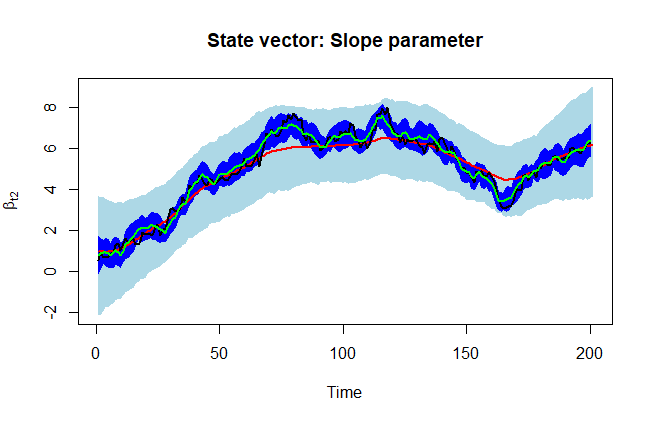
\includegraphics[width=340pt, height=200pt]{Chapters/chapter8/figures/SimSSreg.png}
	\caption[List of figure caption goes here]{Simulation: Dynamic linear model.}\label{fig1}
\end{figure} 

\textbf{Example: Effects of inflation on interest rate I}

We use the dataset \textit{16INTDEF.csv} provided by \cite[Chaps.~10]{wooldridge2016introductory} to study the effects of inflation on interest rate. The specification is $\Delta i_t=\beta_{t1}+\beta_{t2}\Delta inf_t+\beta_{t3}\Delta def_t+\mu_t$ and $\bm{\beta}_t=\bm{\beta}_{t-1}+\bm{w}_t$, where $\Delta z_t=z_{t}-z_{t-1}$ is the difference operator, $i_t$ is the three-month T-bill rate, $inf_t$ is the annual inflation rate based on the consumer price index (CPI), and $def_t$ is the federal budget deficit as percentage of gross domestic product (GDP) from 1948 to 2003 in the USA. In addition, $\mu_t\sim N(0,\sigma^2)$, $\bm{w}_t\sim N(\bm{0},\text{diag}\left\{\omega_1^2,\omega_1^2\right\})$. We assume inverse-gamma distributions for the priors of scale parameters, and set 12000 MCMC iterations, 2000 as burn-in, and 10 the thinning parameter.

The following code shows how to perform this application. We use the variance of the recursive estimation of the OLS to set the hyperparameters of the inverse-gamma distribution for the variance of $\bm{w}_t$, and the OLS estimate of the variance of the model to set the hyperparameters of the distribution of $\sigma^2$.

Figure \ref{fig2} shows the posterior results of the effect of the inflation on the interest rate. This is a fan chart indicating deciles from 10\% to 90\%, the red shadow area shows around the median value, and the black line is the mean value of the state associated with the annual change in inflation. We see that the annual changes in interest rate are weakly positive related to annual changes in inflation. 

\begin{tcolorbox}[enhanced,width=4.67in,center upper,
	fontupper=\large\bfseries,drop shadow southwest,sharp corners]
	\textit{R code. Dynamic linear model: Effects of inflation on interest rate}
	\begin{VF}
		\begin{lstlisting}[language=R]
rm(list = ls()); set.seed(010101)
DataIntRate <- read.csv("https://raw.githubusercontent.com/besmarter/BSTApp/refs/heads/master/DataApp/16INTDEF.csv", sep = ",", header = TRUE, quote = "")
attach(DataIntRate); Xt <- cbind(diff(inf), diff(def))
K <- dim(Xt)[2] + 1; yt <- diff(i3)
T <- length(yt); RegLS <- lm(yt ~ Xt)
SumRegLS <- summary(RegLS); SumRegLS; SumRegLS$sigma^2  
# Recursive OLS
Bp <- matrix(RegLS$coefficients, T, K, byrow = TRUE)
S <- 20
for(t in S:T){
	RegLSt <- lm(yt[1:t] ~ Xt[1:t,])
	Bp[t,] <- RegLSt$coefficients 
}
VarBp <- var(Bp)
# State spece model
ModelReg <- function(par){
	Mod <- dlm::dlmModReg(Xt, dV = exp(par[1]), dW = exp(par[2:(K+1)]), m0 = RegLS$coefficients,
	C0 = diag(VarBp))
	return(Mod)
}
MCMC <- 12000; burnin <- 2000; thin <- 10
gibbsOut <- dlm::dlmGibbsDIG(yt, mod = dlm::dlmModReg(Xt), a.y = 0.1, rate.y = 0.1,
shape.theta = 0.1, rate.theta = 0.1,
n.sample = MCMC,
thin = thin, save.states = TRUE)
B2t <- matrix(0, MCMC - burnin, T + 1)
for(t in 1:(T+1)){
	B2t[,t] <- gibbsOut[["theta"]][t,2,-c(1:burnin)] 
}
dV <- coda::mcmc(gibbsOut[["dV"]][-c(1:burnin)])
dW <- coda::mcmc(gibbsOut[["dW"]][-c(1:burnin),])
summary(dV); summary(dW)
plot(dV); plot(dW)
library(fanplot); library(latex2exp)
df <- as.data.frame(B2t)
plot(NULL, main="Percentiles", xlim = c(1, T+1), ylim = c(-1, 2), xlab = "Time", ylab = TeX("$\\beta_{t1}$"))
fan(data = df); lines(colMeans(B2t), col = "black", lw = 2)
abline(h=0, col = "blue")
\end{lstlisting}
	\end{VF}
\end{tcolorbox}

\begin{figure}[!h]
	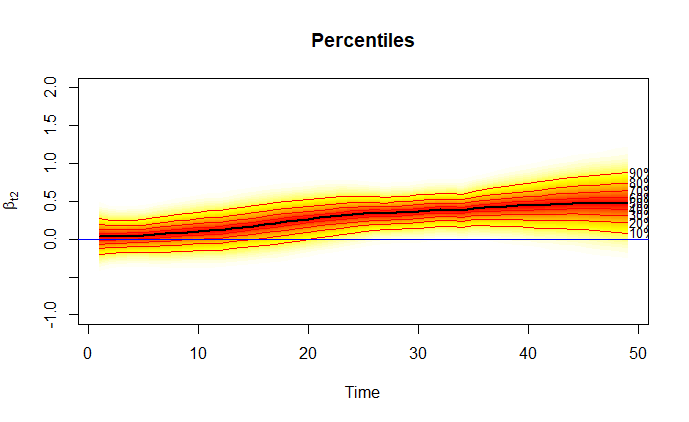
\includegraphics[width=340pt, height=200pt]{Chapters/chapter8/figures/IntInf.png}
	\caption[List of figure caption goes here]{Effects of inflation on interest rate: Dynamic linear model.}\label{fig2}
\end{figure}


We can extend the \textit{dynamic linear model} with \textit{random walk states} to take into account time invariant location parameters. In particular, we follow \cite{de1995simulation}, who propose the \textit{simulation smoother}. This algorithm overcomes some shortcomings of the FFBS algorithm, such as slow convergence and computational overhead. We focus on the case $M=1$, 
\begin{align}
	{Y}_t&=\bm{z}_t^{\top}\bm{\alpha}+\bm{x}_t^{\top}\bm{\beta}_t+\bm{h}_t^{\top}\bm{\epsilon}_t,& t=1,2,\dots,T. & \text{   (Observation equation)}\label{DeJongObs}\\
	\bm{\beta}_t&=\bm{\beta}_{t-1}+\bm{H}_t\bm{\epsilon}_t, & t=1,2,\dots,T. & \text{   (States equations)}\label{DeJongSt},
\end{align}
where $\bm{z}_t$ and $\bm{x}_t$ are $L$-dimensional and $K$-dimensional vectors of regressors associated with time-invariant and time-varying parameters, respectively, $\bm{h}_t$ is a vector of dimension $1+K$, $\bm{H}_t$ is a matrix of dimension $K\times 1+K$, $\bm{\beta}_0=\bm{0}$ and $\bm{\epsilon}_t\sim N(\bm{0}_{1+K},\sigma^2\bm{I}_{1+K})$.

Observe that this specification encompasses Equations \ref{eq1Obs} and \ref{eq1St} setting $\bm{\epsilon}_t=[\mu_t \ \bm{w}_t^{\top}]^{\top}$, $\bm{h}_t=[1 \ 0 \ \dots \ 0]$, $\bm{H}_t=[\bm{0}_K \ \bm{U}_{K\times K}]$ such that $\text{diag}\left\{\omega_1^2 \ \dots \ \omega_K^2\right\}=\sigma^2\bm{U}\bm{U}^{\top}$, $\bm{\alpha}=\bm{0}$, and $\bm{h}_t\bm{H}_t^{\top}=\bm{0}_{K}$.

The nice idea of \cite{de1995simulation} was to propose an efficient algorithm to get draws from $\bm{\eta}_t=\bm{F}_t\bm{\epsilon}_t$, where the most common choice is $\bm{F}_t=\bm{H}_t$, which means drawing samples from the perturbations of the states, and then, recovering the states from Equation \ref{DeJongSt} and $\bm{\beta}_0=\bm{0}$. \cite{de1995simulation} present a more general version of the \textit{state space model} that the one presented here. 

Using the system given by Equations \ref{DeJongObs} and \ref{DeJongSt}, $\bm{F}_t=\bm{H}_t$ and $\bm{h}_t\bm{H}_t^{\top}=\bm{0}_{K}$, the \textit{filtering} recursions are given by $e_t=Y_t-\bm{z}_t^{\top}\bm{\alpha}-\bm{x}_t^{\top}\bm{b}_{t-1}$, ${q}_t=\bm{x}_t^{\top}\bm{B}_{t-1}\bm{x}_t+\bm{h}_t^{\top}\bm{h}_t$, $\bm{K}_t=\bm{B}_{t-1}\bm{x}_tq_t^{-1}$, $\bm{b}_t=\bm{b}_{t-1}+\bm{K}_t e_t$, and $\bm{B}_t=\bm{B}_{t-1}-\bm{B}_{t-1}\bm{x}_t\bm{K}_t^{\top}+\bm{H}_t\bm{H}_t^{\top}$, where $\bm{b}_0=\bm{0}$ and $\bm{B}_0=\bm{H}_0\bm{H}_0^{\top}$. See system 2 in \cite{de1995simulation} for a more general case. We should save $e_t$ (innovation vector), $q_t$ (scale innovation variance) and $\bm{K}_t$ (\textit{Kalman gain}) from this recursion. 

Then, setting $\bm{r}_T=0$ and $\bm{M}_T=\bm{0}$, we run backwards from $t=T-1, T-2, \dots, 1$, the following recursions: $\bm{\Lambda}_{t+1}=\bm{H}_{t+1}\bm{H}_{t+1}^{\top}$, $\bm{C}_{t+1}=\bm{\Lambda}_{t+1}-\bm{\Lambda}_{t+1}\bm{M}_{t+1}\bm{\Lambda}_{t+1}^{\top}$, $\bm{\xi}_{t+1}\sim N(\bm{0}_K,\sigma^2\bm{C}_{t+1})$, $\bm{L}_{t+1}=\bm{I}_K-\bm{K}_{t+1}\bm{x}_{t+1}^{\top}$, $\bm{V}_{t+1}=\bm{\Lambda}_{t+1}\bm{M}_{t+1}\bm{L}_{t+1}$, $\bm{r}_{t}=\bm{x}_{t+1} e_{t+1}/q_{t+1} + \bm{L}_{t+1}^{\top}\bm{r}_{t+1}-\bm{V}_{t+1}^{\top}\bm{C}_{t+1}^{-1}\bm{\xi}_{t+1}$, $\bm{M}_{t}=\bm{x}_{t+1}\bm{x}_{t+1}^{\top}/q_{t+1}+\bm{L}_{t+1}^{\top}\bm{M}_{t+1}\bm{L}_{t+1}+\bm{V}_{t+1}^{\top}\bm{C}_{t+1}^{-1}\bm{V}_{t+1}$, and $\bm{\eta}_{t+1}=\bm{\Lambda}_{t+1}\bm{r}_{t+1}+\bm{\xi}_{t+1}$. \cite{de1995simulation} show that $\bm{\eta}=[\bm{\eta}_1^{\top} \ \dots \ \bm{\eta}_T^{\top}]^{\top}$ is drawn from $p(\bm{H}_t\bm{\epsilon}_t|y_t,\bm{x}_t,\bm{z}_t,\bm{h}_t,\bm{H}_t,\bm{\alpha},\sigma^2, t=1,2,\dots,T)$. Thus, we can recover $\bm{\beta}_t$ using \ref{DeJongSt} and $\bm{\beta}_0=\bm{0}_K$.

We assume in the model given by Equations \ref{DeJongObs} and \ref{DeJongSt} that $\bm{h}_t=[1 \ 0 \ \dots \ 0]^{
\top}$ and $\bm{H}_t=[\bm{0}_K \ \text{diag}\left\{1/\tau_1\dots1/\tau_K\right\}]$, and then perform Bayesian inference assuming independent priors, that is, $\pi(\bm{\beta}_0,\bm{\alpha},\sigma^2,\bm{\tau})=\pi(\bm{\beta}_0)\pi(\bm{\alpha})\pi(\sigma^2)\prod_{k=1}^K\pi(\tau_k^2)$ where $\sigma^2\sim IG(\alpha_0/2,\delta_0/2)$, $\tau_k^2\sim G(v_{0}/2,v_{0}/2)$, $k=1,\dots,K$, $\bm{\alpha}\sim N(\bm{a}_0,\bm{A}_0)$ and $\bm{\beta}_0\sim N(\bm{b}_0,\bm{B}_0)$. The conditional posterior distributions are $\sigma^2|\bm{y},\bm{X},\bm{Z},\bm{\beta}_{0:T},\bm{\alpha},\bm{\tau}\sim IG(\alpha_{n}/2,\delta_n/2)$, where $\delta_n=\sum_{t=1}^T\left[(\bm{\beta}_t-\bm{\beta}_{t-1})^{\top}\bm{\Psi}(\bm{\beta}_t-\bm{\beta}_{t-1})+(y_t-\bm{z}_t^{\top}\bm{\alpha}-\bm{x}_t^{\top}\bm{\beta}_t)^{\top}(y_t-\bm{z}_t^{\top}\bm{\alpha}-\bm{x}_t^{\top}\bm{\beta}_t)\right]+\delta_0$ and  $\alpha_{n}=T(K+1)+\alpha_0$, $\bm{\tau}=[\tau_1 \ \dots \ \tau_K]$, $\bm{\Psi}=\text{diag}\left\{\tau_1^2,\dots,\tau_K^2\right\}$, and $\tau_k^2|\bm{y},\bm{X},\bm{Z},\bm{\beta}_{0:T},\sigma^2\sim G(v_{1n}/2,v_{2kn}/2)$, where $v_{1n}=T+v_{0}$ and $v_{2kn}=\sigma^{-2}\sum_{t=1}^T(\bm{\beta}_{t,k}-\bm{\beta}_{t-1,k})^2+v_{0}$, and $\bm{\alpha}|\bm{y},\bm{X},\bm{Z},\sigma^2,\bm{\beta}_{1:T},\bm{\tau}\sim N(\bm{a}_n,\bm{A}_n)$, where $\bm{A}_n=(\bm{A}_0^{-1}+\sigma^{-2}\sum_{t=1}^T\bm{z}_t\bm{z}_t^{\top})^{-1}$ and $\bm{a}_n=\bm{A}_n(\bm{A}_0^{-1}\bm{a}_0+\sigma^{-2}\sum_{t=1}^T\bm{z}_t(y_t-\bm{x}_t^{\top}\bm{\beta}_t))$. The vector of the dependent variable is $\bm{y}$, and all regressors are in $\bm{X}$ and $\bm{Z}$.

We can see that all the previous posterior distributions are conditional on the state vector $\bm{\beta}_{0:T}$, which can be sampled using the \textit{simulation smoother} algorithm conditional on draws of the time-invariant parameters. Thus, the \textit{state space model} provides an excellent illustration of the modular nature of the Bayesian framework where performing inference of more complex models very often simply involves adding new blocks to a MCMC algorithm. This means we can break down a complex inferential problem into smaller, more manageable parts, this is, a ``divide and conquer" approach. This is possible due to the structure of conditional posterior distributions. Exercise 3 asks to perform a simulation of the model given by Equations \ref{DeJongObs} and \ref{DeJongSt}, and program the MCMC algorithm including the \textit{simulation smoother}.   

\section{ARMA processes}\label{sec82}

Since the seminal work of \cite{box_jenkins_1976}, autoregressive moving average (ARMA) models have become ubiquitous in time series analysis. Thus, we present a brief introduction to these models in this section.

Let's start with the linear Gaussian model with autorregresive errors,
\begin{align}
	Y_t & = \bm{x}_t^{\top}\bm{\beta}+\mu_t\label{eq1}\\
	\phi(L)\mu_t & = \epsilon_t \label{eq2}, 
\end{align}
where $\epsilon_t \stackrel{iid}{\sim} N(0,\sigma^2)$, $\phi(L)=1-\phi_1L-\phi_2L^2-\dots-\phi_pL^p$ is a polynomial in the lag operator ($L$), where $Lz_t=z_{t-1}$, and in general, $L^rz_t=z_{t-r}$.

Thus, we see that stochastic error $\mu_t$ follows an \textit{autoregressive process of order $p$}, that is, $\mu_t\sim AR(p)$. It is standard practice to assume that $\mu_t$ is second-order stationary, this implies that the mean, variance and autocovariance of $\mu_t$ are finite and independent of $t$ and $s$, although $\mathbb{E}[\mu_t\mu_s]$ may depend on $|t-s|$. Then, all roots of $\phi(L)$ lie outside the unit circle, for instance, given an $AR(1)$, then, $1-\phi_1L=0$, implies, $L=1/\phi_1$ such that  $|\phi_1|<0$ for the process being second-order stationary.

The likelihood function conditional on the first $p$ observations is
\begin{align*}
	p(Y_{p+1},\dots,Y_T|y_{p},\dots,y_1,\bm{\theta})&=\prod_{t=p+1}^{T}p(Y_t|H_{t-1},\bm{\theta})\\
	&\propto \sigma^{-(T-p)}\exp\left\{-\frac{1}{2\sigma^2}\sum_{t=p+1}^T(Y_t-\hat{Y}_{t|t-1,\bm{\theta}})^2\right\},
\end{align*} 
where $H_{t-1}$ is the past history, $\bm{\theta}$ collects all parameters ($\bm{\beta}, \phi_1,\dots,\phi_p, \sigma^2$), and $\hat{Y}_{t|t-1,\bm{\theta}}=(1-\phi(L))Y_t+\phi(L)\bm{x}^{\top}\bm{\beta}$.

We can see that multiplying the first expression in Equation \ref{eq1} by $\phi(L)$, we can express the model as 
\begin{align}\label{eq3}
	Y_t^*=\bm{x}_t^{*\top}\bm{\beta}+\epsilon_t
\end{align}
where $Y_t^*=\phi(L)Y_t$ and $\bm{x}_t^{*}=\phi(L)\bm{x}_t$.

Thus, collecting all observations $t=p+1,p+2,\dots,T$, we have $\bm{y}^*=\bm{X}^*\bm{\beta}+\bm{\epsilon}$, where $\bm{\epsilon}\sim N(\bm{0},\sigma^2\bm{I}_{T-p})$, $\bm{y}^*$ is a $T-p$ dimensional vector, and $\bm{X}^*$ is a $(T-p)\times K$ dimensional matrix.

Assuming that $\bm{\beta}|\sigma\sim N(\bm{\beta}_0,\sigma^2\bm{B}_0)$, $\sigma^2\sim IG(\alpha_0/2,\delta_0/2)$ and $\bm{\phi}\sim N(\bm{\phi}_0,\bm{\Phi}_0)\mathbbm{1}[\bm{\phi}\in S_{\bm{\phi}}]$, where $S_{\bm{\phi}}$ is the stationary region of $\bm{\phi}=[\phi_1 \ \dots \ \phi_p]^{\top}$. Then, Equation \ref{eq3} implies that $\bm{\beta}|\sigma^2,\bm{\phi},\bm{y},\bm{X}\sim N(\bm{\beta}_n, \sigma^2{\bm{B}}_n)$, where $\bm{B}_n = (\bm{B}_0^{-1} + \bm{X}^{*\top}\bm{X}^{*})^{-1}$ and $\bm{\beta}_n = \bm{B}_n(\bm{B}_0^{-1}\bm{\beta}_0 + \bm{X}^{*\top}\bm{y}^{*})$. In addition, $\sigma^2|\bm{\beta},\bm{\phi},\bm{y},\bm{X}\sim IG(\alpha_n/2,\delta_n/2)$ where $\alpha_n=\alpha_0+T-p$ and $\delta_n=\delta_0+(\bm{y}^*-\bm{X}^{*}\bm{\beta})^{\top}(\bm{y}^*-\bm{X}^{*}\bm{\beta})+(\bm{\beta}-\bm{\beta}_0)\bm{B}_0^{-1}(\bm{\beta}-\bm{\beta}_0)$. Thus, the previous conditional posterior distributions imply that we can use a Gibbs sampling algorithm to perform inference of these parameters \cite{chib1993bayes}.

We know from Equation \ref{eq1} that $\mu_t=Y_t-\bm{x}_t^{\top}\bm{\beta}$, from Equation \ref{eq2} that $\mu_t=\phi_1\mu_{t-1}+\dots+\phi_p\mu_{t-p}+\epsilon_t$, $t=p+1,\dots,T$. In matrix notation $\bm{\mu}=\bm{U}\bm{\phi}+\bm{\epsilon}$, where $\bm{\mu}$ is a $T-p$ dimensional vector, $\bm{U}$ is a $(T-p)\times p$ matrix whose $t$-th row is $[\mu_{t-1} \ \dots \ \mu_{t-p}]$. Thus, the posterior distribution of $\bm{\phi}|\bm{\beta},\sigma^2,\bm{y},\bm{X}$ is $N(\bm{\phi}_n, \bm{\Phi}_n)\mathbbm{1}[\bm{\phi}\in S_{\bm{\phi}}]$, where $\bm{\Phi}_n=(\bm{\Phi}_0^{-1}+\sigma^{-2}\bm{U}^{\top}\bm{U})$ and $\bm{\phi}_n=\bm{\Phi}_n(\bm{\Phi}_0^{-1}\bm{\phi}_0+\sigma^{-2}\bm{U}^{\top}\bm{\mu})$ (see Exercise 4).

Drawing from the model restricted to stationarity is straightforward: we simply sample from the multivariate normal distribution and discard draws that do not meet the stationarity condition. The proportion of draws that satisfy this restriction represents the conditional probability that the process is stationary.\\

\textbf{Example: Effects of inflation on interest rate II}

We specified a \textit{dynamic linear model} in the example of the effects of inflation on interest rate to take into account a potential dynamic relationship. However, we can consider dynamics in this example assuming  $\Delta i_t=\beta_{1}+\beta_{2}\Delta inf_t+\beta_{3}\Delta def_t+\mu_t$ where $\mu_t=\phi \mu_{t-1} + \epsilon_t$, which implies $\Delta i_t=\beta_{1}(1-\phi_1)+\phi_1\Delta i_{t-1}+\beta_{2}(\Delta inf_t-\phi_1 \Delta inf_{t-1})+\beta_{3}(\Delta def_t-\phi_1 \Delta def_{t-1})+\epsilon_t$. Thus, we use again the dataset \textit{16INTDEF.csv} provided by \cite[Chaps.~10]{wooldridge2016introductory} to provide an illustration of linear regressions with $AR(1)$ errors.

The following code shows how to perform this application using vague priors assuming $\alpha_0=\delta_0=0.01$, $\bm{\beta}_0=\bm{0}$, $\bm{B}_0=\bm{I}$, $\bm{\phi}_0=\bm{0}$ and $\bm{\Phi}_0=\bm{I}$. We use 15000 MCMC iterations plus a burn-in equal 5000, and thin equal to 5. 


\begin{tcolorbox}[enhanced,width=4.67in,center upper,
	fontupper=\large\bfseries,drop shadow southwest,sharp corners]
	\textit{R code. AR(1) model: Effects of inflation on interest rate}
	\begin{VF}
		\begin{lstlisting}[language=R]
rm(list = ls())
set.seed(010101)
DataIntRate <- read.csv("https://raw.githubusercontent.com/besmarter/BSTApp/refs/heads/master/DataApp/16INTDEF.csv", sep = ",", header = TRUE, quote = "")
attach(DataIntRate)
yt <- diff(i3); ytlag <- dplyr::lag(yt, n = 1)
T <- length(yt)
Xt <- cbind(diff(inf), diff(def)); Xtlag <- dplyr::lag(Xt, n = 1)
K <- dim(Xt)[2] + 1
Reg <- lm(yt ~ ytlag + I(Xt[,-1] - Xtlag))
SumReg <- summary(Reg); SumReg
PostSig2 <- function(Beta, Phi){
	Xstar<- matrix(NA, T-1, K - 1)
	ystar <- matrix(NA, T-1, 1)
	for(t in 2:T){
		Xstar[t-1,] <- Xt[t,] - Phi*Xt[t-1,]
		ystar[t-1,] <- yt[t] - Phi*yt[t-1]
	}
	Xstar <- cbind(1, Xstar)
	an <- T - 1 + a0
	dn <- d0 + t(ystar - Xstar%*%Beta)%*%(ystar - Xstar%*%Beta) + t(Beta - b0)%*%B0i%*%(Beta - b0)
	sig2 <- invgamma::rinvgamma(1, shape = an/2, rate = dn/2)
	return(sig2)
}
PostBeta <- function(sig2, Phi){
	Xstar<- matrix(NA, T-1, K - 1)
	ystar <- matrix(NA, T-1, 1)
	for(t in 2:T){
		Xstar[t-1,] <- Xt[t,] - Phi*Xt[t-1,]
		ystar[t-1,] <- yt[t] - Phi*yt[t-1]
	}
	Xstar <- cbind(1, Xstar)
	XtXstar <- t(Xstar)%*%Xstar
	Xtystar <- t(Xstar)%*%ystar
	Bn <- solve(B0i + XtXstar)
	bn <- Bn%*%(B0i%*%b0 + Xtystar)
	Beta <- MASS::mvrnorm(1, bn, sig2*Bn)
	return(Beta)
}
PostPhi <- function(sig2, Beta){
	u <- yt - cbind(1,Xt)%*%Beta
	U <- u[-T]
	ustar <- u[-1]
	UtU <- t(U)%*%U
	Utu <- t(U)%*%ustar
	Phin <- solve(Phi0i + sig2^(-1)*UtU)
	phin <- Phin%*%(Phi0i%*%phi0 + sig2^(-1)*Utu)
	Phi <- truncnorm::rtruncnorm(1, a = -1, b = 1, mean = phin, sd = Phin^0.5)
	return(Phi)
}
		\end{lstlisting}
	\end{VF}
\end{tcolorbox}


\begin{tcolorbox}[enhanced,width=4.67in,center upper,
	fontupper=\large\bfseries,drop shadow southwest,sharp corners]
	\textit{R code. AR(1) model: Effects of inflation on interest rate}
	\begin{VF}
		\begin{lstlisting}[language=R]
# Hyperparameters
d0 <- 0.01; a0 <- 0.01
b0 <- rep(0, K); c0 <- 1; 
B0 <- c0*diag(K); B0i <- solve(B0)
phi0 <- 0; Phi0 <- 1; Phi0i <- 1/Phi0
# MCMC parameters
mcmc <- 15000
burnin <- 5000
tot <- mcmc + burnin
thin <- 1
PostBetas <- matrix(0, mcmc+burnin, K)
PostSigma2s <- rep(0, mcmc+burnin)
PostPhis <- rep(0, mcmc+burnin)
Beta <- rep(0, K); Phi <- 0
sig2 <- SumReg$sigma^2; Phi <- SumReg$coefficients[2,1]
Beta <- SumReg$coefficients[c(1,3,4),1]
pb <- winProgressBar(title = "progress bar", min = 0, max = tot, width = 300)
for(s in 1:tot){
	sig2 <- PostSig2(Beta = Beta, Phi = Phi)
	PostSigma2s[s] <- sig2
	Beta <- PostBeta(sig2 = sig2, Phi = Phi)
	PostBetas[s,] <- Beta
	Phi <- PostPhi(sig2 = sig2, Beta = Beta)
	PostPhis[s] <- Phi
	setWinProgressBar(pb, s, title=paste( round(s/tot*100, 0), "% done"))
}
close(pb)
keep <- seq((burnin+1), tot, thin)
PosteriorBetas <- coda::mcmc(PostBetas[keep,])
summary(PosteriorBetas)
PosteriorSigma2 <- coda::mcmc(PostSigma2s[keep])
summary(PosteriorSigma2)
PosteriorPhi <- coda::mcmc(PostPhis[keep])
summary(PosteriorPhi)
dfBinf <- as.data.frame(PosteriorBetas[,2])
# Basic density
p <- ggplot(dfBinf, aes(x=var1)) + 
geom_density(color="darkblue", fill="lightblue") +
geom_vline(aes(xintercept=mean(var1)), color="blue", linetype="dashed", linewidth=1) +
geom_vline(aes(xintercept=quantile(var1, 0.025)), color="red", linetype="dashed", linewidth=1) +
geom_vline(aes(xintercept=quantile(var1, 0.975)), color="red", linetype="dashed", linewidth=1) +
labs(title="Density effect of inflation on interest rate", x="Effect of inflation", y = "Density")
\end{lstlisting}
	\end{VF}
\end{tcolorbox}

Figure \ref{fig3} shows the posterior density plot of the effects of inflation rate on interest rate. The posterior mean of this coefficient is approximately 0.25, and the credible interval at 95\% is (0, 0.46), which indicates again that the annual changes in interest rate are weakly positive related to annual changes in inflation (see Figure \ref{fig2} as reference). 

\begin{figure}[!h]
	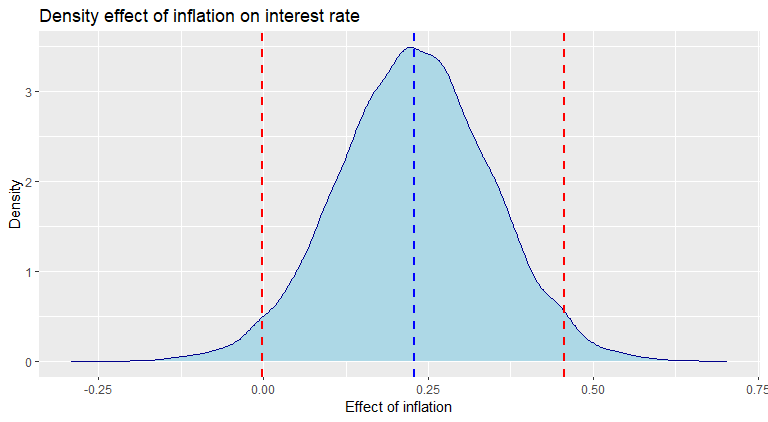
\includegraphics[width=340pt, height=200pt]{Chapters/chapter8/figures/InfInt.png}
	\caption[List of figure caption goes here]{Density: Effects of inflation on interest rate.}\label{fig3}
\end{figure} 


Observe that the previous setting encompasses the particular relevant case  $Y_t\sim AR(p)$, it is just omitting the covariates such that $Y_t=\mu_t$. \cite{chib1994bayes} extend the Bayesian inference of linear regression with $AR(p)$ errors to $ARMA(p,q)$ errors using a \textit{state-space} representation. 

Setting $Y_t=\mu_t$ such that $Y_t=\sum_{s=1}^{p}\phi_jY_{t-s}+\sum_{s=1}^{q}\theta_s \epsilon_{t-s}+\epsilon_t$, letting $r=\max \left\{p,q+1\right\}$, $\phi_s=0$ for $s>p$ and $\theta_s=0$ for $s>q$, and defining the matrices $\bm{x}^{\top}=[1 \ 0 \ \dots \ 0]$, $\bm{H}=[1 \ \psi_1 \ \dots \ \psi_{r-1}]^{\top}$, both are $r$-dimensional vectors, 
\begin{align*}
	\bm{G}=\begin{bmatrix}
		\phi_1 & 1 & 0 & \dots & 0\\
		\phi_2 & 0 & 1 & \dots & 0\\
		\vdots & \vdots & \ddots &  &\\
		\phi_{r-1} & 0 & 0 & \dots & 1\\
		\phi_r & 0 & 0 & \dots & 0\\
	\end{bmatrix} = \begin{bmatrix}
		\phi_1 & \vdots &  &  & \\
		\phi_2 & \vdots &  & \bm{I}_{r-1}  & \\
		\vdots & \vdots &  &  &\\
		\dots & \dots & \dots & \dots & \dots\\
		\phi_r & 0 & 0 & \dots & 0\\
	\end{bmatrix},
\end{align*} 
which is a $r\times r$ dimensional matrix, and give the \textit{state} vector $\bm{\beta}_t=[\beta_{1,t} \ \beta_{2,t} \ \dots \ \beta_{r,t}]^{\top}$, the $ARMA$ model has the following representation:
\begin{align*}
	Y_t&=\bm{x}^{\top}\bm{\beta}_t\\
	\bm{\beta}_t &= \bm{G}\bm{\beta}_{t-1}+\bm{H}\epsilon_{t}.
\end{align*}

This is a \textit{dynamic linear model} where $\bm{\Sigma}_t=0$, and $\bm{\Omega}_t=\sigma^2\bm{H}\bm{H}^{\top}$ (see \cite{petris2009dynamic,chib1994bayes}).

A nice advantage of the \textit{state-space} representation of the $ARMA$ model is that the evaluation of the likelihood can be performed efficiently using the recursive laws. Extensions to autoregressive integrated moving average $ARIMA(p,d,q)$ models can be seen in \cite[Chap.~3]{petris2009dynamic}. In $ARIMA(p,d,q)$ models, $d$ refers to the level of integration (difference) that is required to eliminate the stochastic trend in a time series (see \cite[Chap.~4]{enders_2014} for details).\\

\textbf{Example: $AR(2)$ process}

Let's see the \textit{state-space} representation of a stationary $AR(2)$ process with intercept, that is, $Y_t=\mu+\phi_1Y_{t-1}+\phi_2Y_{t-2}+\epsilon_t$, where $\epsilon_t\sim N(0,\sigma^2)$. Thus, $\mathbb{E}[Y_t]=\frac{\mu}{1-\phi_1-\phi_2}$, and variance $Var[Y_t]=\frac{\sigma^2(1-\phi_2)}{1-\phi_2-\phi_1^2-\phi_1^2\phi_2-\phi_2^2+\phi_2^3}$.

In addition, we can proof that setting $z_t=Y_t-\bar{\mu}$, we have $z_t=\phi_1z_{t-1}+\phi_2z_{t-2}+\epsilon_t$ where $\mathbb{E}[z_t]=0$, and these are equivalent representations (see Exercise 5). Then, setting  $\bm{x}^{\top}=[1 \ 0]$, $\bm{H}=[1 \ 0]^{\top}$, $\bm{G}=\begin{bmatrix}
	\phi_1 & 1\\
	\phi_2 & 0 \\
\end{bmatrix}$, $\bm{\beta}_t=[\beta_{t1} \ \beta_{t2}]^{\top}$, $\bm{\Sigma}_t=0$ and $\bm{\Omega}_t=\sigma^2$ we have
\begin{align*}
	z_t&=\bm{x}^{\top}\bm{\beta}_t& \text{(Observation equations)}\\
	\bm{\beta}_t&=\bm{G}\bm{\beta}_{t-1}+\bm{H}{\epsilon}_t & \text{(States equations)}.
\end{align*}

We use the function \textit{stan\_sarima} from the package \textit{bayesforecast} to perform Bayesian inference in $ARMA$ models in our GUI. The following code shows how to simulate an $AR(2)$ process, and perform Bayesian inference using this function.

\begin{tcolorbox}[enhanced,width=4.67in,center upper,
	fontupper=\large\bfseries,drop shadow southwest,sharp corners]
	\textit{R code. Simulation and inference: AR(2) model}
	\begin{VF}
		\begin{lstlisting}[language=R]
rm(list = ls()); set.seed(010101)
T <- 200; mu <- 0.5 
phi1 <- 0.5; phi2 <- 0.3; sig <- 0.5
Ey <- mu/(1-phi1-phi2); Sigy <- sig*((1-phi2)/(1-phi2-phi1^2-phi2*phi1^2-phi2^2+phi2^3))^0.5 
y <- rnorm(T, mean = Ey, sd = Sigy)
e <- rnorm(T, mean = 0, sd = sig)
for(t in 3:T){
	y[t] <- mu + phi1*y[t-1] + phi2*y[t-2] + e[t]
}
mean(y); sd(y)
y <- ts(y, start=c(1820, 1), frequency=1)
plot(y)
iter <- 10000; burnin <- 5000; thin <- 1; tot <- iter + burnin
library(bayesforecast)
sf1 <- bayesforecast::stan_sarima(y, order = c(2, 0, 0), prior_mu0 = normal(0, 1),
prior_ar = normal(0, 1), prior_sigma0 = inverse.gamma(0.01/2, 0.01/2),
seasonal = c(0, 0, 0), iter = tot, warmup = burnin, chains = 1)
keep <- seq(burnin+1, tot, thin)
Postmu <- sf1[["stanfit"]]@sim[["samples"]][[1]][["mu0"]][keep]
Postsig <- sf1[["stanfit"]]@sim[["samples"]][[1]][["sigma0"]][keep]
Postphi1 <- sf1[["stanfit"]]@sim[["samples"]][[1]][["ar0[1]"]][keep]
Postphi2 <- sf1[["stanfit"]]@sim[["samples"]][[1]][["ar0[2]"]][keep]
Postdraws <- coda::mcmc(cbind(Postmu, Postsig, Postphi1, Postphi2))
summary(Postdraws)
Quantiles for each variable:
            	2.5%    25%    50%    75%  97.5%
Postmu   0.39914 0.5732 0.6625 0.7518 0.9346
Postsig  0.47696 0.5071 0.5248 0.5439 0.5829
Postphi1 0.42384 0.5159 0.5634 0.6089 0.6979
Postphi2 0.06034 0.1456 0.1920 0.2361 0.3286
plot(Postdraws)
\end{lstlisting}
	\end{VF}
\end{tcolorbox}
We perform 10000 MCMC iterations plus a burn-in equal 5000 assuming $\sigma^2\sim IG(0.01/2, 0.01/2)$, $\mu\sim N(0, 1)$ and $\phi_k\sim N(0, 1)$, $k=1,2$. The trace plots look well, and all 95\% credible intervals encompass the population values.

Algorithm \ref{alg:ARMA} shows how to do perform inference in $ARMA(p,q)$ models using our GUI. See also Chapter \ref{chapGUI} for details regarding the dataset structure. 

\begin{algorithm}[h!]
	\caption{Autoregressive Moving Average ($ARMA$) models}\label{alg:ARMA}
	\begin{algorithmic}[1]  		 			
		\State Select \textit{Time series Model} on the top panel
		\State Select \textit{ARMA} using the left radio button
		\State Upload the dataset selecting first if there is header in the file, and the kind of separator in the \textit{csv} file of the dataset (comma, semicolon, or tab). Then, use the \textit{Browse} button under the \textbf{Choose File} legend
		\State Select MCMC iterations, burn-in and thinning parameters using the \textit{Range sliders}
		\State Set the order of the $ARMA$ model, $p$ and $q$ parameters
		\State Set the location and scale hyperparameters of the \textit{intercept}, autoregressive ($AR$), moving average ($MA$) and standard deviation. Take into account that there is just one set of hyperparameters for $AR$ and $MA$ coefficients. This step is not necessary as by default our GUI uses non-informative priors
		\State Click the \textit{Go!} button
		\State Analyze results
		\State Download posterior chains and diagnostic plots using the \textit{Download Posterior Chains} and \textit{Download Posterior Graphs} buttons
	\end{algorithmic} 
\end{algorithm}

The function \textit{stan\_sarima} uses software \textit{Stan} \cite{Stan2024}, which in turn uses \textit{Hamiltonian Monte Carlo} (HMC). The following code shows how to perform Bayesian inference in the $AR(2)$ model programming the HMC from scratch. We should clarify that this is only an illustration as HMC is less efficient than the Gibbs sampler in this example. However, HMC can outperform traditional MCMC algorithms in more complex models, especially when dealing with high-dimensional probability distributions or when MCMC struggles with poor mixing due to posterior correlation.

We perform the simulation in the first block setting $\mu=0.5$, $\phi_1=0.5$, $\phi_2=0.3$ and $\sigma=0.25$, and the sample size equal 200. Then, we set the hyperparameters, and the function to calculate the logarithm of the posterior distribution. We parametrize the model using $\tau = \log(\sigma^2)$ such that $\sigma^2=\exp\left\{\tau\right\}$, consequently, avoiding issues due to the restriction of non-negativity of $\sigma^2$. Thus, we must take into account the Jacobian due to the transformation, that is $d\sigma^2/d\tau=\exp(\tau)$. Then, we have the function to calculate the gradient vector of the log posterior distribution. We should calculate the gradient vector analytically because using finite difference can be computationally expensive. However, it can be a good idea to check the analytical calculations evaluation the function at the maximum posterior estimate, where this function should return values near 0, or compare results with finite differences in a few evaluation points.

The posterior distribution is given by\footnote{Take into account that we do not consider the first two observations when present the likelihood, this is no an issue when there is a large sample size.}
\begin{align*}
	\pi(\mu,\phi_1,\phi_2,\tau|\bm{y})&\propto \prod_{t=3}^T(\exp(\tau))^{-1/2}\exp\left\{-\frac{1}{2\exp(\tau)}(y_t-\mu-\phi_1y_{t-1}-\phi_2y_{t-2})^2\right\}\\
	&\times\exp\left\{-\frac{1}{2\sigma^2_{\mu}}(\mu-\mu_0)^2\right\}\times\exp\left\{-\frac{1}{2\sigma^2_{\phi_1}}(\phi_1-\phi_{10})^2\right\}\\
	&\times\exp\left\{-\frac{1}{2\sigma^2_{\phi_2}}(\phi_2-\phi_{20})^2\right\}\times\exp\left\{-(\alpha_0/2+1)\tau\right\}\exp\left\{-\delta_0/(2\exp(\tau))\right\}\exp(\tau).
\end{align*} 

The components of the gradient vector of the log posterior distribution are given by
\begin{align*}
	\frac{\partial \log(\pi(\mu,\phi_1,\phi_2,\tau|\bm{y}))}{\partial\mu}&=\frac{\sum_{t=3}^T(y_t-\mu-\phi_1y_{t-1}-\phi_2y_{t-2})}{\exp(\tau)}-\frac{1}{\sigma_{\mu}^2}(\mu-\mu_0)\\
	\frac{\partial\log(\pi(\mu,\phi_1,\phi_2,\tau|\bm{y}))}{\partial\phi_1}&=\frac{\sum_{t=3}^T(y_t-\mu-\phi_1y_{t-1}-\phi_2y_{t-2})y_{t-1}}{\exp(\tau)}-\frac{1}{\sigma_{\phi_1}^2}(\phi_1-\phi_{10})\\
	\frac{\partial\log(\pi(\mu,\phi_1,\phi_2,\tau|\bm{y}))}{\partial\phi_2}&=\frac{\sum_{t=3}^T(y_t-\mu-\phi_1y_{t-1}-\phi_2y_{t-2})y_{t-2}}{\exp(\tau)}-\frac{1}{\sigma_{\phi_2}^2}(\phi_2-\phi_{20})\\	\frac{\partial\log(\pi(\mu,\phi_1,\phi_2,\tau|\bm{y}))}{\partial\tau}&=-\frac{(T-2)}{2}+\frac{\sum_{t=3}^T(y_t-\mu-\phi_1y_{t-1}-\phi_2y_{t-2})^2}{2\exp(\tau)}\\
	&-(\alpha_0/2+1)+\delta_0/(2\exp(\tau))+1.\\
\end{align*}

Then, we have the code for the Hamiltonian Monte Carlo as given in Chapter \ref{chap5}. We set the initial values equal to $\mu=\bar{y}=1/(T-2)\sum_{t=3}^T y_t$, $\phi_1=\phi_2=0$ and $\exp((1/(T-2))\sum_{t=3}^T(y_t-\bar{y})^2)$, and $M$ equal to the inverse covariance matrix of the posterior distribution evaluated at the maximum a posterior estimate. In addition, $\epsilon$ is randomly draw from a uniform distribution between 0 and 2$\epsilon_0$, and $L$ is the highest integer near to $1/\epsilon$, this to approximately satisfy $L\epsilon=1$. 

We can check that all 95\% credible intervals encompass the population values, and the posterior means are near the population values. The acceptance rate is higher than 65\% on average, thus we should increase the base step ($\epsilon_0$). In addition, we do not impose the stationary conditions on $\phi_1$ and $\phi_2$. Exercise 6 asks to program a HMC taking into account these requirements.

\begin{tcolorbox}[enhanced,width=4.67in,center upper,
	fontupper=\large\bfseries,drop shadow southwest,sharp corners]
	\textit{R code. Simulation and inference: AR(2) model using Hamiltonian Monte Carlo}
	\begin{VF}
		\begin{lstlisting}[language=R]
# Simulation AR(2)
rm(list = ls()); set.seed(010101); T <- 1000; K <- 4 
mu <- 0.5; phi1 <- 0.5; phi2 <- 0.3; sig <- 0.5 
Ey <- mu/(1-phi1-phi2); Sigy <- sig*((1-phi2)/(1-phi2-phi1^2-phi2*phi1^2-phi2^2+phi2^3))^0.5 
y <- rnorm(T, mean = Ey, sd = Sigy); e <- rnorm(T, mean = 0, sd = sig)
for(t in 3:T){
	y[t] <- mu + phi1*y[t-1] + phi2*y[t-2] + e[t]
}
# Hyperparameters
d0 <- 0.01; a0 <- 0.01; mu0 <- 0; MU0 <- 1
phi0 <- c(0, 0); Phi0 <- diag(2)
# Log posterior multiply by -1 to use optim
LogPost <- function(theta, y){
	mu <- theta[1]; phi1 <- theta[2]; phi2 <- theta[3]
	tau <- theta[4]; sig2 <- exp(tau); logLik <- NULL
	for(t in 3:T){
		logLikt <- dnorm(y[t], mean = mu + phi1*y[t-1] + phi2*y[t-2], sd = sig2^0.5, log = TRUE)
		logLik <- c(logLik, logLikt)
	}
	logLik <- sum(logLik)
	logPrior <- dnorm(mu, mean = mu0, sd = MU0^0.5, log = TRUE) + dnorm(phi1, mean = phi0[1], sd = Phi0[1,1]^0.5, log = TRUE) + dnorm(phi2, mean = phi0[2], sd = Phi0[2,2]^0.5, log = TRUE) + invgamma::dinvgamma(sig2, shape = a0/2, rate = d0/2, log = TRUE)
	logPosterior <- logLik + logPrior + tau
	return(-logPosterior) # Multiply by -1 to minimize using optim
}
theta0 <- c(mean(y), 0, 0, var(y))
Opt <- optim(theta0, LogPost, y = y, hessian = TRUE)
theta0 <- Opt$par; VarPost <- solve(Opt$hessian)
# Gradient log posterior
GradientTheta <- function(theta, y){
	mu <- theta[1]; phi1 <- theta[2]; phi2 <- theta[3]
	tau <- theta[4]; sig2 <- exp(tau); SumLik <- matrix(0, 3, 1)
	SumLik2 <- NULL
	for(t in 3:T){
		xt <- matrix(c(1, y[t-1], y[t-2]), 3, 1)
		SumLikt <- (y[t] - (mu + phi1*y[t-1] + phi2*y[t-2]))*xt
		SumLik2t <- (y[t] - (mu + phi1*y[t-1] + phi2*y[t-2]))^2
		SumLik <- rowSums(cbind(SumLik, SumLikt))
		SumLik2 <- sum(SumLik2, SumLik2t)
	}
	Grad_mu <- SumLik[1]/sig2 - (1/MU0)*(mu - mu0)
	Grad_phi1 <- SumLik[2]/exp(tau) - 1/Phi0[1,1]*(phi1 - phi0[1])
	Grad_phi2 <- SumLik[3]/exp(tau) - 1/Phi0[2,2]*(phi2 - phi0[2])
	Grad_tau <- -(T-2)/2 + SumLik2/(2*exp(tau)) - (a0/2 + 1) + d0/(2*exp(tau)) + 1 
	Grad <- c(Grad_mu, Grad_phi1, Grad_phi2, Grad_tau)
	return(Grad)
}
\end{lstlisting}
	\end{VF}
\end{tcolorbox}

\begin{tcolorbox}[enhanced,width=4.67in,center upper,
	fontupper=\large\bfseries,drop shadow southwest,sharp corners]
	\textit{R code. Simulation and inference: AR(2) model using Hamiltonian Monte Carlo}
	\begin{VF}
		\begin{lstlisting}[language=R]
# Hamiltonian Monte Carlo function
HMC <- function(theta, y, epsilon, M){
	L <- ceiling(1/epsilon)
	Minv <- solve(M); thetat <- theta
	K <- length(thetat)
	mom <- t(mvtnorm::rmvnorm(1, rep(0, K), M))
	logPost_Mom_t <- -LogPost(thetat, y) +  mvtnorm::dmvnorm(t(mom), rep(0, K), M, log = TRUE)  
	for(l in 1:L){
		if(l == L){
			mom <- mom + 0.5*epsilon*GradientTheta(theta, y)
			theta <- theta + epsilon*Minv%*%mom
		}else{
			mom <- mom + epsilon*GradientTheta(theta, y)
			theta <- theta + epsilon*Minv%*%mom
		}
	}
	logPost_Mom_star <- -LogPost(theta, y) +  mvtnorm::dmvnorm(t(mom), rep(0, K), M, log = TRUE)  
	alpha <- min(1, exp(logPost_Mom_star-logPost_Mom_t))
	u <- runif(1)
	if(u <= alpha){
		thetaNew <- c(theta)
	}else{
		thetaNew <- thetat
	}
	rest <- list(theta = thetaNew, Prob = alpha)
	return(rest)
}
# Posterior draws
S <- 1000; burnin <- 1000; thin <- 2; tot <- S + burnin
thetaPost <- matrix(NA, tot, K)
ProbAcept <- rep(NA, tot)
theta0 <- c(mean(y), 0, 0, exp(var(y))) 
M <- solve(VarPost); epsilon0 <- 0.1
pb <- winProgressBar(title = "progress bar", min = 0, max = tot, width = 300)
for(s in 1:tot){
	epsilon <- runif(1, 0, 2*epsilon0)
	L <- ceiling(1/epsilon)
	HMCs <- HMC(theta = theta0, y, epsilon, M) 
	theta0 <- HMCs$theta 
	thetaPost[s,] <- HMCs$theta
	ProbAcept[s] <- HMCs$Prob
	setWinProgressBar(pb, s, title=paste( round(s/tot*100, 0), "% done"))
}
close(pb)
keep <- seq((burnin+1), tot, thin)
thetaF <- coda::mcmc(thetaPost[keep,])
summary(thetaF)
summary(exp(thetaF[,K]))
ProbAceptF <- coda::mcmc(ProbAcept[keep])
summary(ProbAceptF)
\end{lstlisting}
	\end{VF}
\end{tcolorbox} 
    
\section{Stochastic volatility models}\label{sec83}
A notable example of non-linear and non-Gaussian \textit{state-space models} is stochastic volatility models (SVMs), which are widely used to model the volatility of financial returns. SVMs have gained significant attention due to their flexibility, ability to capture complex dynamics such as asymmetries, and ease of generalization to simultaneously model multiple returns, making them advantageous over generalized autoregressive conditional heteroskedasticity (GARCH) models proposed by \cite{bollerslev_1986}. However, estimating SVMs is more challenging than estimating GARCH models. This is because GARCH models determine variance in a deterministic manner, whereas SVMs do so stochastically. Consequently, GARCH models are typically estimated using maximum likelihood methods, while SVMs require Bayesian approaches, adding complexity to the estimation process.

The specification of the stochastic volatility model is given by
\begin{align}
	y_t&=\bm{x}_t^{\top}\bm{\beta}+\exp\left\{0.5h_t\right\}\mu_t& \text{(Observation equation)}\label{eqsvobs}\\
	h_t&=\mu+\phi(h_{t-1}-\mu)+\sigma w_t& \text{(State equation)}\label{eqsvst},
\end{align}
where $y_t$ are the log-returns, $\bm{x}_t$ are controls, $\bm{\beta}$ are time-invariant location parameters, $\mu_t\sim N(0,1)$, $w_t\sim N(0,1)$, $\mu_t\perp w_t$, the initial log-variance process $h_0\sim N(\mu, \sigma^2/(1-\phi^2))$, $\mu$, $\phi$ and $\sigma$ are the level, persistence and standard deviation of the log-variance, respectively.

Given the specification in Equations \ref{eqsvobs} and \ref{eqsvst}, we can write down the observation equation as $\log\left\{(y_t-\bm{x}_t^{\top}\bm{\beta})^2\right\}=h_t+\log(\mu_t^2)$, thus there is now a linear, but non-Gaussian \textit{state-space model}. \cite{kastner2014ancillarity} approximate the distribution of $\log(\mu_t^2)$ by a mixture of normal distributions, that is, $\log(\mu_t^2)|l_t\sim N(m_{l_t},s_{l_t}^2)$, $l_r\in \left\{1,2,\dots,10\right\}$ defines the mixture component indicator at time $t$. Thus, $\log\left\{(y_t-\bm{x}_t^{\top}\bm{\beta})^2\right\}=h_t+\log(\mu_t^2)$ and $h_t=\mu+\phi(h_{t-1}-\mu)+\sigma w_t$ can be written as a linear and conditionally Gaussian \textit{state-space model}, where $\log\left\{(y_t-\bm{x}_t^{\top}\bm{\beta})^2\right\}=m_{l_t}+h_t+\mu_t^2$, $\mu_t\sim N(0, s_{l_t}^2)$.        

We use the \textit{stochvol} package in our GUI to perform MCMC inference in the SVMs \cite{hosszejni_kastner_2021}; this package in turn is based on the MCMC algorithms proposed by \cite{kastner2014ancillarity}. The default prior distributions in the \textit{stochvol} package are $\bm{\beta}\sim N(\bm{b}_0,\bm{B}_0)$, $\mu\sim N(\mu_0,\sigma_{\mu0}^2)$, $(\phi+1)/2\sim B(\alpha_0,\beta_0)$, and $\sigma^2\sim G(1/2,1/(2\sigma^2_{\sigma^2}))$. The prior distribution of $\phi$ is set to achieve stationarity of the process ($\phi\in(-1,1)$). Most of applications find $\phi\approx 1$, thus authors of the package recommend to set $\alpha_0 \gtrsim 5$ and $\beta_0\approx 1.5$. The prior distribution of $\sigma^2$ is equivalent to $\sigma\sim |N(0,\sigma^2_{\sigma^2})|$ (half-normal distribution); this is recommended by the authors as the convenient conjugate inverse-gamma distribution does not work well due to bounding $\sigma$ away from 0, which is no a good feature when modeling the log-variance of log-returns.

The following code shows how to simulate and perform Bayesian inference in the stochastic volatility model using the function \textit{svsample} from the \textit{stochvol} package. We set the stochastic volatility parameters $\mu=-10$, $\phi=0.95$ and $\sigma=0.3$. We assume two regressors that distribute standard normal, $\bm{\beta}=[0.5 \ 0.3]^{\top}$, and the sample size is 1250, which is approximately having daily returns during 5 years. We use the default hyperparameters, 10000 MCMC iterations, a burn-in equal 5000 and a thin parameter equal 5.

The summary statistics of the posterior draws show that all 95\% credible intervals encompass the population parameters, and posterior chains seem to achieve convergence. Figure \ref{fig4} displays the posterior results of the volatility ($h_t$). The posterior mean (blue) follow the ``observed" series (black), and the 95\% credible intervals (light blue) encompass most of the time the ``observed" series. 

\begin{tcolorbox}[enhanced,width=4.67in,center upper,
	fontupper=\large\bfseries,drop shadow southwest,sharp corners]
	\textit{R code. Simulation and inference: Stochastic volatility model}
	\begin{VF}
		\begin{lstlisting}[language=R]
rm(list = ls()); set.seed(010101)
T <- 1250; K <- 2
X <- matrix(rnorm(T*K), T, K)
B <- c(0.5, 0.3); mu <- -10; phi <- 0.95; sigma <- 0.3
h <- numeric(T); y <- numeric(T)
h[1] <- rnorm(1, mu, sigma / sqrt(1 - phi^2))  # Initial state
y[1] <- X[1,]%*%B + rnorm(1, 0, exp(h[1] / 2))           # Initial observation
for (t in 2:T) {
	h[t] <- mu + phi*(h[t-1]-mu) + rnorm(1, 0, sigma)
	y[t] <- X[t,]%*%B + rnorm(1, 0, sd = exp(0.5*h[t]))
}
df <- as.data.frame(cbind(y, X))
colnames(df) <- c("y", "x1", "x2")
MCMC <- 10000; burnin <- 10000; thin <- 5
res <- stochvol::svsample(y, designmatrix = X, draws = MCMC, burnin = burnin, thin = thin, priormu = c(0, 100), priorsigma = c(1), priorphi = c(5, 1.5), priorbeta =  c(0, 10000))
summary(res[["para"]][[1]][,-c(4,5)])
summary(res[["beta"]])
ht <- res[["latent"]][[1]]
library(dplyr)
library(ggplot2)
library(latex2exp)
ggplot2::theme_set(theme_bw())
x_means <- colMeans(ht)
x_quantiles <- apply(ht, 2, function(x) quantile(x, probs = c(0.025, 0.975)))
df <- tibble(t = seq(1, T), mean = x_means, lower = x_quantiles[1, ], upper = x_quantiles[2, ], x_true = h, observations = y)
plot_filtering_estimates <- function(df) {
	p <- ggplot(data = df, aes(x = t)) + geom_ribbon(aes(ymin = lower, ymax = upper), alpha = 1, fill = "lightblue") + geom_line(aes(y = x_true), colour = "black", alpha = 1, linewidth = 0.5) + geom_line(aes(y = mean), colour = "blue", linewidth = 0.5) + 	ylab(TeX("$h_{t}$")) + xlab("Time")
	print(p)
}
plot_filtering_estimates(df)
\end{lstlisting}
	\end{VF}
\end{tcolorbox} 

\begin{figure}[!h]
	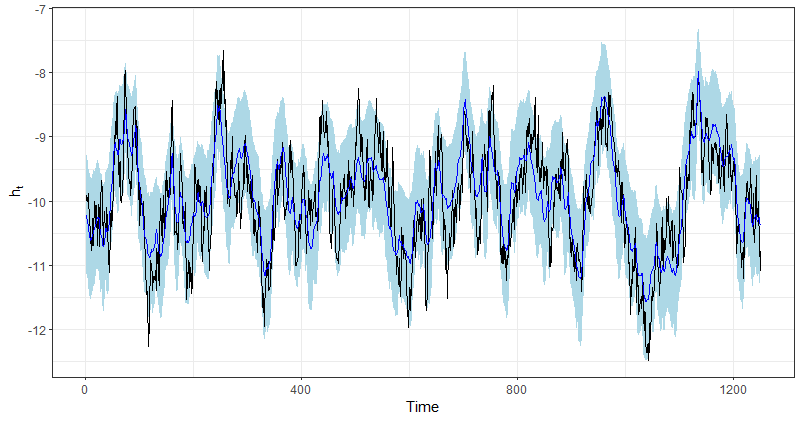
\includegraphics[width=340pt, height=200pt]{Chapters/chapter8/figures/SVmodel.png}
	\caption[List of figure caption goes here]{Stochastic volatility model.}\label{fig4}
\end{figure} 

So far, we have used MCMC algorithms to perform inference in \textit{state-space models}. These algorithms require all observations to estimate the unknown parameters, a process referred to as offline or batch inference. However, this approach has limitations when online inference is needed, as every new observation requires simulating a new posterior chain. This is because MCMC algorithms do not naturally adapt to sequential updates. In contrast, particle filter algorithms, which are a subset of sequential Monte Carlo (SMC) methods, are specifically designed for sequential use, making them suitable for online inference.    
     
Remember from Chapter \ref{chap5} that particle filters (sequential Monte Carlo) are algorithms that allow computing a numerical approximation to the filtering distribution $\pi(\bm{\theta}_{1:t}|\bm{y}_{1:t})$ sequentially in time. This is particularly relevant in non-linear and non-Gaussian models where there is no analytical solution for the filtering distribution.

The following code shows how to perform SMC in the vanilla stochastic volatility model assuming that the proposal distribution is the conditional prior distribution, that is, $q(h_t|h_{t-1},y_t)=\pi(h_t|h_{t-1})$, which is normal with mean $\mu+\phi(h_{t-1}-\mu)$ and variance $\sigma^2$. This choice implies that the incremental importance weights are equal to $p(y_t|h_t)$, which is $N(0,\exp(h_t))$. Therefore, the weights are proportional to the likelihood function. We perform multinomial resampling every time period in the code, and start the algorithm in the stationary distribution of $h_t$. Remember that there are other resampling approaches that are more efficient, for instance, residual resampling. See Chapter \ref{chap5} for details. We ask in Exercise 7 to modify this code to perform resampling when the effective sample size is lower than 50\% of the number of particles. In addition, we ask to program a sequential importance sampling, and check why is important to perform resampling in this simple example. 

Figure \ref{fig5} illustrates the filtering recursion using SMC with uneven weights (blue line), even weights (purple line), bands corresponding to plus/minus two standard deviations (light blue shading), and the true state (black line).\footnote{This standard deviation estimates the conditional posterior's standard deviation derived from the particles, not the estimator's standard deviation. The latter requires several independent particle runs on the same data.} The results indicate that SMC performs well even in a simple implementation, with no significant differences between using even and uneven weights (see Chapter \ref{chap5}).

In this example we use the population parameters to perform the filtering recursion. However, this is no the case in practice, that is, we have to estimate the time invariant parameters. Therefore, there are more elaborate algorithms to achieve this (see Chapter \ref{chap5}). For instance, \cite{andrieu2010pmcmc} propose particle Markov chain Monte Carlo, this is a family of methods that combines MCMC and SMC. See \cite{dahlin2019getting} for a tutorial of particle Metropolis-Hastings in \textbf{R}. A potential practical solution, for applications that require a sequential updating of a posterior distribution over an unbounded time horizon, is to estimate offline the time invariant parameters using MCMC algorithms up to a specific time period, and then update sequentially online the state vector during subsequent time periods, and iterate this process. This is not optimal, but it can be practical.  

\begin{tcolorbox}[enhanced,width=4.67in,center upper,
	fontupper=\large\bfseries,drop shadow southwest,sharp corners]
	\textit{R code. Simulation and inference: Stochastic volatility model programming sequential Monte Carlo from scratch}
	\begin{VF}
		\begin{lstlisting}[language=R]
rm(list = ls()); set.seed(010101)
T <- 1250; mu <- -10; phi <- 0.95; sigma <- 0.3
h <- numeric(T); y <- numeric(T)
h[1] <- rnorm(1, mu, sigma / sqrt(1 - phi^2))  
y[1] <- rnorm(1, 0, exp(h[1] / 2))           
for (t in 2:T) {
	h[t] <- mu + phi*(h[t-1]-mu) + rnorm(1, 0, sigma)
	y[t] <- rnorm(1, 0, sd = exp(0.5*h[t]))
}
N <- 10000
log_Weights <- matrix(NA, N, T)  # Log weights
Weights <- matrix(NA, N, T)  # Weights 
WeightsST <- matrix(NA, N, T)  # Normalized weights 
WeightsSTT <- matrix(1/N, N, T)  # Normalized weights bar 
particles <- matrix(NA, N, T)   # Particles
particlesT <- matrix(NA, N, T)   # Particles bar
logalphas <- matrix(NA, N, T)   # Incremental importance 
particles[, 1] <- rnorm(N, mu, sigma / sqrt(1 - phi^2))  # Stationary prior
log_Weights[, 1] <- dnorm(y[1], 0, sd = exp(0.5*particles[,1]), log = TRUE)  # Likelihood
Weights[, 1] <- exp(log_Weights[, 1])
WeightsST[, 1] <- Weights[, 1] / sum(Weights[, 1])
ESS[1] <- (sum(WeightsST[, 1]^2))^(-1)
ind <- sample(1:N, size = N, replace = TRUE, prob = WeightsST[, 1]) # Resample 
particles[, 1] <- particles[ind, 1] # Resampled particles
particlesT[, 1] <- particles[, 1] # Resampled particles
WeightsST[, 1] <- rep(1/N, N) # Resampled weights
pb <- winProgressBar(title = "progress bar", min = 0, max = T, width = 300)
for (t in 2:T) {
	particles[, t] <- rnorm(N, mu + phi*(particles[, t - 1] - mu), sigma)  # Sample from proposal
	logalphas[, t] <- dnorm(y[t], 0, sd = exp(0.5*particles[,t]), log = TRUE) 
	Weights[, t] <- exp(logalphas[, t])
	WeightsST[, t] <- Weights[, t] / sum(Weights[, t])
	if(t < T){
		ind <- sample(1:N, size = N, replace = TRUE, prob = WeightsST[, t])
		particles[, 1:t] <- particles[ind, 1:t]
	}else{
		ind <- sample(1:N, size = N, replace = TRUE, prob = WeightsST[, t])
		particlesT[, 1:t] <- particles[ind, 1:t]
	}
	setWinProgressBar(pb, t, title=paste( round(t/T*100, 0), "% done"))
}
close(pb)
\end{lstlisting}
	\end{VF}
\end{tcolorbox}

\begin{tcolorbox}[enhanced,width=4.67in,center upper,
	fontupper=\large\bfseries,drop shadow southwest,sharp corners]
	\textit{R code. Simulation and inference: Stochastic volatility model programming sequential Monte Carlo from scratch}
	\begin{VF}
		\begin{lstlisting}[language=R]
FilterDist <- colSums(particles * WeightsST)
SDFilterDist <- (colSums(particles^2 * WeightsST) - FilterDist^2)^0.5
FilterDistT <- colSums(particlesT * WeightsSTT)
SDFilterDistT <- (colSums(particlesT^2 * WeightsSTT) - FilterDistT^2)^0.5
MargLik <- colMeans(Weights)
plot(MargLik, type = "l")
library(dplyr)
library(ggplot2)
require(latex2exp)
ggplot2::theme_set(theme_bw())
Tfig <- 250
keepFig <- 1:Tfig
df <- tibble(t = keepFig,
mean = FilterDist[keepFig],
lower = FilterDist[keepFig] - 2*SDFilterDist[keepFig],
upper = FilterDist[keepFig] + 2*SDFilterDist[keepFig],
meanT = FilterDistT[keepFig],
lowerT = FilterDistT[keepFig] - 2*SDFilterDistT[keepFig],
upperT = FilterDistT[keepFig] + 2*SDFilterDistT[keepFig],
x_true = h[keepFig])
plot_filtering_estimates <- function(df) {
	p <- ggplot(data = df, aes(x = t)) +
	geom_ribbon(aes(ymin = lower, ymax = upper), alpha = 1,
	fill = "lightblue") +
	geom_line(aes(y = x_true), colour = "black", alpha = 1,
	linewidth = 0.5) +
	geom_line(aes(y = mean), colour = "blue", linewidth = 0.5) +
	geom_line(aes(y = meanT), colour = "purple", linewidth = 0.5) +
	ylab(TeX("$h_{t}$")) + xlab("Time")
	print(p)
}
plot_filtering_estimates(df)
\end{lstlisting}
	\end{VF}
\end{tcolorbox} 

 
\begin{figure}[!h]
	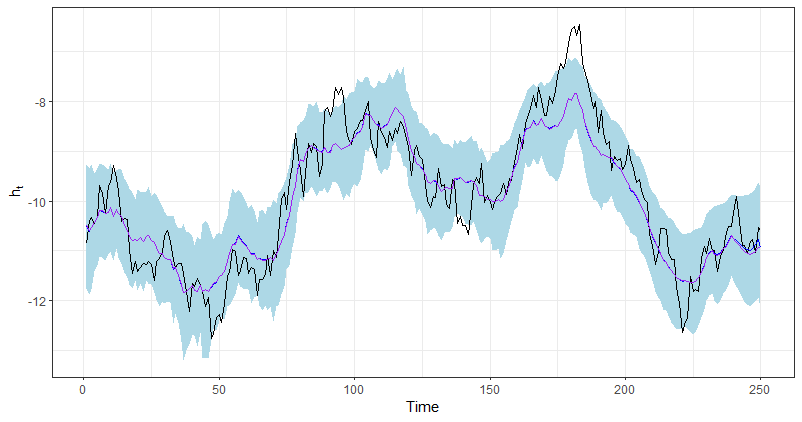
\includegraphics[width=340pt, height=200pt]{Chapters/chapter8/figures/SVSMC.png}
	\caption[List of figure caption goes here]{Stochastic volatility model: Sequential Monte Carlo (SMC).}\label{fig5}
\end{figure} 
  
\section{Vector Autoregressive models}\label{sec84}
Another widely used methodological approach in time series analysis is the vector autoregressive (VAR) model, which extends AR(p) models to the multivariate case. Since the seminal work by Sims (1980) \cite{sims1980macroeconomics}, these models have become a cornerstone of macroeconomic research. This chapter provides an introduction to Bayesian inference in VAR models, with detailed discussions available in \cite{koop2010bayesian,DelNegro2011VAR,wozniak2016bayesian}.

The \textit{reduced-form} VAR(p) model can be written as
\begin{align}\label{eqVAR}
	\bm{Y}_t=\bm{v} + \sum_{j=1}^p\bm{A}_{j}\bm{Y}_{t-j}+\bm{\mu}_t,
\end{align}
where $\bm{Y}_t$ is a $M$-dimensional vector having information of $M$ time series variables, $\bm{v}$ is a $M$-dimensional vector of intercepts, $\bm{A}_{j}$ are $M\times M$ matrices of coefficients, and $\bm{\mu}_t \stackrel{iid}{\sim} N_M(\bm{0}, \bm{\Sigma})$ stochastic errors, $t=1,2,\dots,T$ and $j=1,2,\dots,p$. Other deterministic terms and exogenous variables can be added to the specification without main difficulty, we do not do this to keep simply the notation. In addition, we assume that the stability condition is satisfied such that the stochastic process is stationary (see \cite[Chap.~2]{helmut2005new} for details). 

Following the matrix-form notation of the multivariate regression model (see sections \ref{sec44} and \ref{sec71}), we can set $\bm{Y}=\left[{\bm{Y_{1}}} \ {\bm{Y_{2}}} \ \ldots \ {\bm{Y_{M}}}\right]$, which is an $ T\times M$ matrix, $\bm{x}_t=[1 \ \bm{Y}_{t-1}^{\top} \ \dots \ \bm{Y}_{t-p}^{\top}]$ is a $(1+Mp)$-dimensional row vector, we define $K=1+Mp$ to facilitate notation, and set \begin{align*}
\bm{X}=\begin{bmatrix}
	\bm{x}_1\\
	\bm{x}_2\\
	\vdots \\
	\bm{x}_T\\
\end{bmatrix},
\end{align*}
which is a $ T\times K$ matrix, $\bm{B}=\left[\bm{v} \ \bm{A}_{1} \ \bm{A}_{2} \ldots \bm{A}_{P}\right]^{\top}$ is a $ K \times M$ matrix of parameters, and $\bm{U}=\left[\bm{\mu}_{1} \ \bm{\mu}_{2}\ldots \bm{\mu}_{M}\right]$ is a $T\times M$-dimensional matrix of stochastic random errors such that $\bm{U}\sim N_{T\times M}(\bm{0}_{T\times M},\bm{\Sigma}\otimes \bm{I}_T)$. Thus, we can express the VAR(p) model in the form of a multivariate regression model,
\begin{align*}
	\bm{Y}=\bm{X}\bm{B}+\bm{U}.
\end{align*}
We can assume conjugate priors to facilitate computation, that is, $\pi({\bm{B}},{\bm{\Sigma}})=\pi({\bm{B}}|{\bm{\Sigma}})\pi({\bm{\Sigma}})$ where $\pi({\bm{B}}|{\bm \Sigma})\sim N_{K\times M}({\bm{B}}_{0},{\bm{V}}_{0},{\bm{\Sigma}})$ and $\pi({\bm{\Sigma}})\sim IW({\bm{\Psi}}_{0},\alpha_{0})$. Thus, $\pi({\bm{B}},{\bm \Sigma}| {\bm{Y}}, {\bm{X}})=\pi ({\bm{B}}| {\bm \Sigma},{\bm{Y}},{\bm{X}})\pi({\bm \Sigma}| {\bm{Y}},{\bm{X}})$ where ${\bm{B}}| {\bm \Sigma},{\bm{Y}}, {\bm{X}} \sim N_{K\times M}({\bm{B}}_n,{\bm{V}}_n,{\bm \Sigma})$ and ${\bm \Sigma}| {\bm{Y}},{\bm{X}} \sim IW({\bm{\Psi}}_n,{\alpha}_n)$, ${\bm{B}}_n = ({\bm{V}}_{0}^{-1}+{\bm{X}}^{\top}{\bm{X}})^{-1}({\bm{V}}_{0}^{-1}{\bm{B}}_{0}+{\bm{X}}^{\top}{\bm{X}}\widehat{\bm{B}})$, ${\bm{V}}_n = ({\bm{V}}_{0}^{-1}+{\bm{X}}^{\top}{\bm{X}})^{-1}$, ${\bm{\Psi}}_n={\bm{\Psi}}_{0}+{\bm{S}}+{\bm{B}}_{0}^{\top}{\bm{V}}_{0}^{-1}{\bm{B}}_{0}+\widehat{\bm{B}}^{\top}{\bm{X}}^{\top}{\bm{X}}\widehat{\bm{B}}-{\bm{B}}_n^{\top}{\bm{V}}_n^{-1}{\bm{B}}_n$, ${\bm{S}}= ({\bm{Y}}-{\bm{X}}\widehat{\bm{B}})^{\top}({\bm{Y}}-{\bm{X}}\widehat{\bm{B}})$, $\widehat{\bm{B}}= ({\bm{X}}^{\top}{\bm{X}})^{-1}{\bm{X}}^{\top}{\bm{Y}}$, and  $\alpha_n= T+\alpha_{0}$. 

We also know from Section \ref{sec44} that the marginal posterior distribution of $\bm{B}$ is $T_{K\times M}({\bm{B}}_n,{\bm{V}}_n,{\bm{\Psi}}_n)$ with $\alpha_n+1-M$ degrees of freedom, and the predictive density of ${\bm{Y}}_{T+1}$ given ${\bm{Y}}$, $\pi({\bm{Y}}_{T+1}|{\bm{Y}})$ is a matrix (multivariate) t distribution $T_{1,M}(\alpha_n-M+1,{\bm{x}}_{T+1}{\bm{B}}_n,1+{\bm{x}}_{T+1}{\bm{V}}_n{\bm{x}}_{T+1}^{\top},{\bm{\Psi}}_n)$.

Thus, we see that once we write a VAR(p) model in the right way, we can perform Bayesian inference as we did in the multivariate regression model. However, assuming conjugate priors has some limitations. First, VAR(p) models have many parameters, for instance, 4 lags and 6 variables, implies 150 ($(1 + 6\times4)\times 6)$) location parameters plus 21 ($6\times(6+1)/2$) scale parameters of the covariance matrix, this implies loss of precision due to macroeconomic data no having large sample sizes regularly. Thus, it is desirable to impose prior restrictions in the specification of the model. This cannot be done using conjugate priors. Second, natural conjugate priors do not allow for flexible extensions such as having different regressors in different equations. Third, the prior structure implies that the prior covariance of the coefficients in any two equations must be proportional each other, this is because the prior covariance form is $\bm{\Sigma}\otimes \bm{V}_0$. However, this does not make sense in some applications, for instance, imposing prior zero restrictions in some coefficients would imply that the prior variance of these coefficients should be near zero. However, this has not to be the case for all coefficients in the model.

Thus, we can tackle the first previous issue by thinking about the VAR(p) specification as we did in the seemingly unrelated equations (SUR) model, where we have different regressors in different equations, and account for unobserved dependence. Thus, we can impose zero restrictions in the VAR(p) model improving its parsimony. Following the setting of Section \ref{sec72}, we have $\bm{Y}_{m}=\bm{Z}_{m}\bm{\beta}_m+\bm{\mu}_{m}$, where $\bm{Y}_m$ is a $T$-dimensional vector corresponding to time series variable $m$-th, $\bm{Z}_m$ is a matrix of dimension $T\times K_m$ of regressors, $\bm{\beta}_m$ is a $K_m$-dimensional vector of location parameters, and $\bm{\mu}_m$ is a $T$-dimensional vector of stochastic errors, $m=1,2,\dots,M$. 

Stacking the $M$ equations, we can write $\bm{y}=\bm{Z}\bm{\beta}+\bm{\mu}$ where $\bm{y}=\left[\bm{Y}_{1}^{\top} \ \bm{Y}_{2}^{\top} \dots \bm{Y}_{M}^{\top}\right]^{\top}$ is a $MT$-dimensional vector,  $\bm{\beta}=\left[\bm{\beta}_{1}^{\top} \ \bm{\beta}_{2}^{\top} \ldots \bm{\beta}_{M}^{\top}\right]^{\top}$ is a $ K$ dimensional vector, $K=\sum_{m=1}^{M} K_m$, $\bm{X}$ is an $MT\times K$ block diagonal matrix composed of $\bm{Z}_{m}$, that is,
\begin{align*}
	\bm{Z}&=\begin{bmatrix}
		\bm{Z}_1 & \bm{0} & \dots & \bm{0}\\
		\bm{0} & \bm{Z}_2 & \dots & \bm{0}\\
		\vdots & \vdots & \ddots & \vdots\\
		\bm{0} & \bm{0} & \dots & \bm{Z}_M		
	\end{bmatrix},
\end{align*}
and $\bm{\mu}=\left[\bm{\mu}_{1}^{\top} \ \bm{\mu}_{2}^{\top} \dots \ \bm{\mu}_{M}^{\top}\right]^{\top}$ is a $MT$-dimensional vector of stochastic errors such that $\bm{\mu}\sim{N}(\bm{0},\bm{\Sigma}\otimes \bm{I}_T)$.

We can use independent priors in this model to overcome the limitations of the conjugate prior, that is, $\pi(\bm{\beta})\sim{N}(\bm{\beta}_0,\bm{B}_0)$ and $\pi(\bm{\Sigma}^{-1})\sim{W}(\alpha_0,\bm{\Psi}_0)$. Thus, we know from Section \ref{sec72} that the posterior distributions are
\begin{equation*}
	\bm{\beta}|\bm{\Sigma}, \bm{y}, \bm{Z} \sim {N}(\bm{\beta}_n, \bm{B}_n), 
\end{equation*}
\begin{equation*}
	\bm{\Sigma}^{-1}|\bm{\beta}, \bm{y}, \bm{Z} \sim {W}(\alpha_n, \bm{\Psi}_n),
\end{equation*}

where $\bm{B}_n=(\bm{Z}^{\top}(\bm{\Sigma}^{-1}\otimes \bm{I}_T )\bm{Z}+\bm{B}_0^{-1})^{-1}$, $\bm{\beta}_n=\bm{B}_n(\bm{B}_0^{-1}\bm{\beta}_0 + \bm{Z}^{\top}(\bm{\Sigma}^{-1}\otimes \bm{I}_T)\bm{y})$, $\alpha_n = \alpha_0 + T$ and $\bm{\Psi}_n = (\bm{\Psi}_0^{-1} + \bm{U}^{\top}\bm{U})^{-1}$, where $\bm{U}$ is an $T\times M$ matrix whose columns are $\bm{Y}_m-\bm{Z}_m\bm{\beta}_m$.

Observe that we have standard conditional posteriors, thus, we can employ a Gibbs sampling algorithm to get the posterior draws. We can calculate the prediction $\bm{y}_{T+1}=[Y_{1T+1} \ Y_{2T+1} \ \dots \ Y_{MT+1}]^{\top}$ knowing that $\bm{y}_{T+1}\sim N(\bm{Z}_{T}\bm{\beta},\bm{\Sigma})$, where \begin{align*}
	\bm{Z}_T&=\begin{bmatrix}
		\bm{z}_{1T}^{\top} & 0 & \dots & 0\\
		0 & \bm{z}_{2T}^{\top} & \dots & 0\\
		\vdots & \vdots & \ddots & \vdots\\
		0 & 0& \dots & \bm{z}_{MT}^{\top}		
	\end{bmatrix},
\end{align*} 
and using the posterior draws of $\bm{\beta}^{(s)}$ and $\bm{\Sigma}^{(s)}$, $s=1,2,\dots,S$. We can also perform inference of functions of the parameters that are of main interest when using VAR models.

Note that the independent priors allow more flexibility regarding prior information. For instance, we can set $\bm{\Psi}_0 = \bm{S}^{-1}$, $\alpha_0=T$, $\bm{\beta}_0=\bm{0}$ and $\bm{B}_0$ as a diagonal matrix, where the variance of the components associated with the coefficients in the $m$-th equation are such that the prior variance of the coefficients of the own-lags are $a_1/l^2$, variances on lag l of variable $m\neq j$ are $a_2s_{m}/(l^2s_{j})$, and variance of the intercepts are set $a_3s_{m}$, $l=1,2,\dots,p$, where $s_{m}$ is the estimated standard error of the residuals in an unrestricted univariate autoregression of variable $m$ versus a constant and its $p$ lags \cite{litterman1986forecasting,koop2010bayesian}. Note that setting $a_1>a_2$ implies that own lags are more important to be good predictors than lags of other variables, and dividing by $l^2$ implies that recent lags are more relevant that further past lags. The specific choice of $a_1$, $a_2$ and $a_3$ ($a_k>0,k=1,2,3$) depends on each application, but it is easier to elicit these parameters rather than the $K(K+1)/2$ different components of $\bm{B}_0$. This setting is named the \textit{Minnesota prior}, as is based on the seminal proposals of Bayesian VAR models by researchers at the University of Minnesota and the Federal Reserve Bank of Minneapolis \cite{doan1984forecasting,litterman1986forecasting}.\footnote{In the case that the variables are not stationary, which is more probable when using variables in levels, like gross domestic product, $\bm{\beta}_0=\bm{0}$, except in the elements associated with the first own lags of the dependent variable of each equation, where the prior mean equals 1.} 

An important function when performing VAR analysis is the \textit{impulse response} function, which is, the response of one variable to an impulse in another variable in the model. The \textit{impulse response} function can be deduced using the $MA$ representation of the VAR model. In particular, we can write Equation \ref{eqVAR} using the lag operator (see Section \ref{sec82}),
\begin{align}\label{eqVAR1}
	\bm{Y}_t=\bm{v} + (\bm{A}_{1}L+\bm{A}_{2}L^2+\dots+\bm{A}_{p}L^p)\bm{Y}_t+\bm{\mu}_t,
\end{align}
thus $\bm{A}(L)\bm{Y}_t=\bm{v}+\bm{\mu}_t$, where $\bm{A}(L)=\bm{I}_M-\bm{A}_{1}L-\bm{A}_{2}L^2-\dots-\bm{A}_{p}L^p$. Let $\bm{\Phi}(L):= \sum_{s=0}^{\infty}\bm{\Phi}_sL^s$ an operator such that $\bm{\Phi}(L)\bm{A}(L)=\bm{I}_M$. Thus, we have that  $\bm{\Phi}(L)\bm{A}(L)\bm{Y}_t=\left(\sum_{s=0}^{\infty}\bm{\Phi}_sL^s\right)\bm{v}+\left(\sum_{s=0}^{\infty}\bm{\Phi}_sL^s\right)\bm{\mu}_{t}=\bm{\mu}+\sum_{s=0}^{\infty}\bm{\Phi}_s\bm{\mu}_{t-s}$. Note that $L^s\bm{v}=\bm{v}$ because $\bm{v}$ is constant, thus we set $\sum_{s=0}^{\infty}\bm{\Phi}_sL^s\bm{v}=\sum_{s=0}^{\infty}\bm{\Phi}_s\bm{v}=\bm{\Phi}(1)\bm{v}=(\bm{I}_M-\bm{A}_{1}-\bm{A}_{2}-\dots-\bm{A}_{p})^{-1}\bm{v}:=\bm{\mu}$, which is the mean of the process \cite[Chap.~2]{helmut2005new}. Therefore, the MA representation of the VAR is
\begin{align}\label{eqMA}
	\bm{Y}_t=\bm{\mu} + \sum_{s=0}^{\infty}\bm{\Phi}_s\bm{\mu}_{t-s},
\end{align}
where $\bm{\Phi}_0=\bm{I}_M$, and we can get the coefficients in $\bm{\Phi}_s$ by the recursion $\bm{\Phi}_s=\sum_{l=1}^s\bm{\Phi}_{s-l}\bm{A}_l$, $\bm{A}_l=\bm{0}$, $l>p$ and $s=1,2,..$ \cite[Chap.~2]{helmut2005new}.

The MA coefficients contain the impulse responses of the system. In particular, $\phi_{mj,s}$, which is the $mj$-th element of the matrix $\bm{\Phi}_s$, represents the response of the $m$-th variable to a unit shock of the variable $j$ in the system, $s$ periods ago, provided that the effect is not contaminated by other shocks in the system. The long-term effects (total multipliers) are given by $\bm{\Psi}_{\infty}:=\sum_{s=1}^{\infty}\bm{\Phi}_s=(\bm{I}_M-\bm{A}_{1}-\bm{A}_{2}-\dots-\bm{A}_{p})^{-1}$.

An assumption in these \textit{impulse response} functions is that a shock occurs in only one variable at a time. This can be questionable as different shocks may be correlated, consequently, occurring simultaneously. Thus, the \textit{impulse response} analysis can be performed based on the alternative MA representation, $\bm{Y}_t=\bm{\mu} + \sum_{s=0}^{\infty}\bm{\Phi}_s\bm{P}\bm{P}^{-1}\bm{\mu}_{t-s}=\bm{\mu} + \sum_{s=0}^{\infty}\bm{\Theta}_s\bm{w}_{t-s}$, where $\bm{\Theta}_s=\bm{\Phi}_s\bm{P}$ and $\bm{w}_{t}=\bm{P}^{-1}\bm{\mu}_{t}$, $\bm{P}$ is a lower triangular matrix such that $\bm{\Sigma}=\bm{P}\bm{P}^{\top}$. Note that the covariance matrix of $\bm{w}_t$ is $\bm{I}_M$ due to $\mathbb{E}[\bm{w}_t\bm{w}_t^{\top}]=\mathbb{E}[\bm{P}^{-1}\bm{\mu}_{t}\bm{\mu}_t^{\top}(\bm{P}^{-1})^{\top}]=\bm{P}^{-1}\bm{\Sigma}(\bm{P}^{-1})^{\top}=\bm{P}^{-1}\bm{P}\bm{P}^{\top}(\bm{P}^{-1})^{\top}=\bm{I}_M$. 

In this representation is sensible to assume that each shock occurs independently due to the covariance matrix of $\bm{w}_t$ being an identity. In addition, a unit shock is a shock of size one standard deviation due the result of the covariance matrix. This is named the \textit{ortogonalized impulse response}, where $\theta_{mj,s}$, which is the $mj$-th element of the matrix $\bm{\Theta}_s$, represents the response of the $m$-th variable to a standard deviation shock of the variable $j$ in the system, $s$ periods ago. The critical point with the ortogonalized impulse responses is that the order of the variables in the VAR is really important because implicitly establishes a recursive model, that is, the $m$-th equation in the system may contain $Y_{1t}, Y_{2t}, \dots, Y_{m-1t}$, but not $Y_{mt}, Y_{m+1t}, \dots, Y_{Mt}$ on the hand-right side of its equation. Thus, $Y_{mt}$ cannot have an instantaneous impact on $Y_{jt}$ for $j<m$ \cite[Chap.~2]{helmut2005new}.

Beyond the fascinating macroeconomic implications embedded in the specification of VAR models, the key point for this section is that we can infer impulse response functions using posterior draws.\\

\textbf{Example: Simulation exercise}

      
 
\section{Summary}\label{sec85}

\section{Exercises}\label{sec86}

\begin{enumerate}
	\item Simulate the \textit{dynamic linear model} assuming $X_t\sim N(1, 0.1\sigma^2)$, $w_t\sim N(0, 0.5\sigma^2)$, $\mu_t\sim N(0, \sigma^2)$, $\beta_0=1$, ${B}_0=0.5\sigma^2$, $\sigma^2=0.25$, and ${G}_t=1$, $t=1,\dots,100$. Then, perform the filtering recursion fixing $\Sigma=25\times 0.25$, $\Omega_1=0.5\Sigma$ (high signal-to-noise ratio) and  $\Omega_2=0.1\Sigma$ (low signal-to-noise ratio). Plot and compare the results. 	
	
	\item Simulate the \textit{dynamic linear model} $y_t=\beta_t x_t + \mu_t$, $\beta_t=\beta_{t-1}+w_t$, where $x_t\sim N(1, 0.1\sigma^2)$, $w_t\sim N(0, 0.5\sigma^2)$, $\mu_t\sim N(0, \sigma^2)$, $\beta_0=0$, $B_0=0.5\sigma^2$, and $\sigma^2=1$, $t=1,\dots,100$. Perform the filtering and smoothing recursions from scratch. 	
	
	\item Simulate the process $y_t=\alpha z_t + \beta_t x_t + \bm{h}^{\top}\bm{\epsilon}_t$, $\beta_t=\beta_{t-1}+\bm{H}^{\top}\bm{\epsilon}_t$, where $\bm{h}^{\top}=[1 \ 0]$, $\bm{H}^{\top}=[0 \ 1/\tau]$, $\bm{v}_t\sim N(\bm{0}_2, \sigma^2\bm{I}_2)$, $x_t\sim N(1, 2\sigma^2)$, $z_t\sim N(0, 2\sigma^2)$, $\alpha=2$, $\tau^2=5$ and $\sigma^2=0.1$, $t=1,\dots,200$. Assume $\pi({\beta}_0,{\alpha},\sigma^2,{\tau})=\pi({\beta}_0)\pi({\alpha})\pi(\sigma^2)\pi(\tau^2)$ where $\sigma^2\sim IG(\alpha_0/2,\delta_0/2)$, $\tau^2\sim G(v_{0}/2,v_{0}/2)$, ${\alpha}\sim N({a}_0,{A}_0)$ and ${\beta}_0\sim N({b}_0,{B}_0)$ such that $\alpha_0=\delta_0=1$, $v_0=5$, $a_0=0$, $A_0=1$, $\beta_0=0$, $B_0=\sigma^2/\tau^2$. Program the MCMC algorithm including the \textit{simulation smoother}.
	
	\item Show that the posterior distribution of $\bm{\phi}|\bm{\beta},\sigma^2,\bm{y},\bm{X}$ in the model $Y_t=\bm{x}_t^{\top}\bm{\beta}+\mu_t$ where $\phi(L)\mu_t=\epsilon_t$ and $\epsilon_t\stackrel{iid}{\sim}N(0,\sigma^2)$ is $N(\bm{\phi}_n, \bm{\Phi}_n)\mathbbm{1}[\bm{\phi}\in S_{\bm{\phi}}]$, where $\bm{\Phi}_n=(\bm{\Phi}_0^{-1}+\sigma^{-2}\bm{U}^{\top}\bm{U})$, $\bm{\phi}_n=\bm{\Phi}_n(\bm{\Phi}_0^{-1}\bm{\phi}_0+\sigma^{-2}\bm{U}^{\top}\bm{\mu})$, and $S_{\phi}$ is the stationary region of $\bm{\phi}$.	  
	
	\item Show that in the $AR(2)$ stationary process, $Y_t=\mu+\phi_1Y_{t-1}+\phi_2Y_{t-2}+\epsilon_t$, where $\epsilon_t\sim N(0,\sigma^2)$, $\mathbb{E}[Y_t]=\frac{\mu}{1-\phi_1-\phi_2}$, and $Var[Y_t]=\frac{\sigma^2(1-\phi_2)}{1-\phi_2-\phi_1^2-\phi_1^2\phi_2-\phi_2^2+\phi_2^3}$.
	
	\item Program a Hamiltonian Monte Carlo taking into account the stationary restrictions on $\phi_1$ and $\phi_2$, and $\epsilon_0$ such that the acceptance rate is near 65\%. 
	
	\item \textbf{Stochastic volatility model}
	\begin{itemize}
		\item Program a sequential importance sampling (SIS) from scratch in the vanilla stochastic volatility model setting $\mu=-10$, $\phi = 0.95$, $\sigma=0.3$ and $T=250$. Check what happen with its performance.
		\item Modify the sequential Monte Carlo (SMC) to perform multinomial resampling when the effective sample size is lower than 50\% the number of particles.  
	\end{itemize}

	\item Estimate the vanilla stochastic volatility model using the dataset \textit{17ExcRate.csv} provided by \cite{ramirez2024testing} of the exchange rate log daily returns from USD/EUR, USD/GBP and GBP/EUR one year before and after the WHO declared the COVID-19 pandemic on 11 March 2020. 
	
	
\end{enumerate}

\chapter{Longitudinal/Panel data models}\label{chap9}

\section{Solutions of Exercises}\label{sec91}
\begin{enumerate}[leftmargin=*]

	\item Show that the posterior distribution of $\bm{\beta}|\sigma^2,\bm{D}$ is $N(\bm{\beta}_n,\bm{B}_n)$, where $\bm{B}_n = (\bm{B}_0^{-1} +\sum_{i=1}^N \bm{X}_i^{\top}\bm{V}_i^{-1}\bm{X}_i)^{-1}$, $\bm{\beta}_n= \bm{B}_n(\bm{B}_0^{-1}\bm{\beta}_0 + \sum_{i=1}^N\bm{X}_i^{\top}\bm{V}_i^{-1}\bm{y}_i)$.
	
	\textbf{Answer}

{\footnotesize	
	\begin{align*}
		\pi(\bm{\beta}|\sigma^2, \bm{D},\bm{y},\bm{X},\bm{W}) & \propto \exp\left\{-\frac{1}{2}\sum_{i=1}^N(\bm{y}_i-\bm{X}_i\bm{\beta})^{\top}\bm{V}_i^{-1}(\bm{y}_i-\bm{X}_i\bm{\beta})\right\}\\
		&\times \exp\left\{-\frac{1}{2}(\bm{\beta}-\bm{\beta}_0)^{\top}\bm{B}_0^{-1}(\bm{\beta}-\bm{\beta}_0)\right\}\\
		& \propto \exp\left\{-\frac{1}{2}\left(-2\bm{\beta}^{\top}\left(\sum_{i=1}^N\bm{X}_i^{\top}\bm{V}_i^{-1}\bm{y}_i+\bm{B}_0^{-1}\bm{\beta}_0\right)+\bm{\beta}^{\top}\left(\sum_{i=1}^N\bm{X}_i^{\top}\bm{V}_i^{-1}\bm{X}_i+\bm{B}_0^{-1}\right)\bm{\beta}\right)\right\}\\
		& = \exp\left\{-\frac{1}{2}(-2\bm{\beta}^{\top}\bm{B}_n^{-1}\bm{B}_n\left(\sum_{i=1}^N\bm{X}_i^{\top}\bm{V}_i^{-1}\bm{y}_i+\bm{B}_0^{-1}\bm{\beta}_0\right)+\bm{\beta}^{\top}\bm{B}_n^{-1}\bm{\beta})\right\}\\
		& = \exp\left\{-\frac{1}{2}(-2\bm{\beta}^{\top}\bm{B}_n^{-1}\bm{\beta}_n+\bm{\beta}^{\top}\bm{B}_n^{-1}\bm{\beta})\right\}. 
	\end{align*} 
}

We can complete the square in this expression by adding and subtracting $\bm{\beta}_n^{\top}\bm{B}_n^{-1}\bm{\beta}_n$. Thus,

	\begin{align*}
	\pi(\bm{\beta}|\sigma^2, \bm{D},\bm{y},\bm{X},\bm{W}) & \propto \exp\left\{-\frac{1}{2}(-2\bm{\beta}^{\top}\bm{B}_n^{-1}\bm{\beta}_n+\bm{\beta}^{\top}\bm{B}_n^{-1}\bm{\beta}+\bm{\beta}_n^{\top}\bm{B}_n^{-1}\bm{\beta}_n-\bm{\beta}_n^{\top}\bm{B}_n^{-1}\bm{\beta}_n)\right\}\\
	&\propto \exp\left\{-\frac{1}{2}(\bm{\beta}-\bm{\beta}_n)^{\top}\bm{B}_n^{-1}(\bm{\beta}-\bm{\beta}_n)\right\}.
\end{align*} 
This is the kernel of a multivariate random variable with mean $\bm{\beta}_n$ and variance matrix $\bm{B}_n$.
	
	\item \textbf{The relation between productivity and public investment example continues}

\begin{itemize}
	\item Perform inference of this example using our GUI.
	\item Program from scratch a Gibbs sampling algorithm to perform this application.
	\item Perform inference in this example assuming that $\mu_{it}|\tau_{it}\sim N(0, \sigma^2/\tau_{it})$ and $\tau_{it}\sim G(v/2,v/2)$ setting $v=5$ 
\end{itemize}

\textbf{Answer}
\begin{tcolorbox}[enhanced,width=4.67in,center upper,
	fontupper=\large\bfseries,drop shadow southwest,sharp corners]
	\textit{R code. The relationship between productivity and public investment, programming from scratch the Gibbs sampler}
	\begin{VF}
		\begin{lstlisting}[language=R]
rm(list = ls())
set.seed(12345)
DataGSP <- read.csv("DataApplications/8PublicCap.csv", sep = ",", header = TRUE, fileEncoding = "latin1")
attach(DataGSP)
K1 <- 5; K2 <- 1
N <- length(unique(id))
y <- log(gsp)
X <- cbind(1, log(pcap), log(pc), log(emp), unemp)
W <- 1
WtW <- t(W)%*%W
table(id)
T <- 17
it <- rep(1, T)
# Hyperparameters
b0 <- rep(0, K1); B0 <- diag(K1); B0i <- solve(B0)
r0 <- 5; R0 <- diag(K2)
a0 <- 0.001; d0 <- 0.001
# MCMC parameters
mcmc <- 10000
burnin <- 5000
tot <- mcmc + burnin
thin <- 1
# Gibbs functions
PostBeta <- function(sig2, D){
	Vi <- sig2*diag(T) + as.numeric(D)*it%*%t(it)
	ViInv <- solve(Vi)
	XVX <- matrix(0, K1, K1)
	XVy <- matrix(0, K1, 1)
	for(i in 1:N){
		ids <- which(id == i)
		Xi <- X[ids, ]
		XVXi <- t(Xi)%*%ViInv%*%Xi
		XVX <- XVX + XVXi
		yi <- y[ids]
		XVyi <- t(Xi)%*%ViInv%*%yi
		XVy <- XVy + XVyi
	}
	Bn <- solve(B0i + XVX)
	bn <- Bn%*%(B0i%*%b0 + XVy)
	Beta <- MASS::mvrnorm(1, bn, Bn)
	return(Beta)
}\end{lstlisting}
	\end{VF}
\end{tcolorbox}


\begin{tcolorbox}[enhanced,width=4.67in,center upper,
	fontupper=\large\bfseries,drop shadow southwest,sharp corners]
	\textit{R code. The relationship between productivity and public investment, programming from scratch the Gibbs sampler}
	\begin{VF}
		\begin{lstlisting}[language=R]
Postb <- function(Beta, sig2, D){
	Di <- solve(D)
	Bni <- solve(sig2^(-1)*WtW + Di)
	bis <- NULL
	for(i in 1:N){
		ids <- which(id == i)
		Xi <- X[ids, ]
		yi <- y[ids]
		Wi <- it
		Wtei <- sig2^(-1)*t(Wi)%*%(yi - Xi%*%Beta)
		bni <- Bni%*%Wtei
		bi <- MASS::mvrnorm(1, bni, Bni)
		bis <- c(bis, bi)
	}
	return(bis)
}
PostSig2 <- function(Beta, D, bs){
	an <- a0 + 0.5*N*T
	ete <- 0
	for(i in 1:N){
		ids <- which(id == i)
		Xi <- X[ids, ]
		yi <- y[ids]
		Wi <- it
		ei <- yi - Xi%*%Beta - bs[i]*Wi
		etei <- t(ei)%*%ei
		ete <- ete + etei
	}
	dn <- 1/d0 + 0.5*ete 
	sig2 <- invgamma::rinvgamma(1, shape = an, scale = dn)
	return(sig2)
}
PostD <- function(bs){
	rn <- r0 + N
	btb <- 0
	for(i in 1:N){
		bsi <- bs[i]
		btbi <- bsi%*%t(bsi)
		btb <- btb + btbi
	}
	Rn <- R0 + btb
	Sigma <- LaplacesDemon::rinvwishart(nu = rn, S = Rn)
	return(Sigma)
}\end{lstlisting}
	\end{VF}
\end{tcolorbox}

\begin{tcolorbox}[enhanced,width=4.67in,center upper,
	fontupper=\large\bfseries,drop shadow southwest,sharp corners]
	\textit{R code. The relationship between productivity and public investment, programming from scratch the Gibbs sampler}
	\begin{VF}
		\begin{lstlisting}[language=R]
PostBetas <- matrix(0, tot, K1)
PostDs <- matrix(0, tot, K2*(K2+1)/2)
PostSig2s <- rep(0, tot)
Postbs <- matrix(0, tot, N)
Beta <- rep(1, K1)
D <- diag(K2)
RegLS <- lm(log(gsp)~log(pcap)+log(pc)+log(emp)+unemp)
SumLS <- summary(RegLS)
sig2 <- SumLS[["sigma"]]^0.5
pb <- winProgressBar(title = "progress bar", min = 0, max = tot, width = 300)
for(s in 1:tot){
	bs <- Postb(Beta = Beta, sig2 = sig2, D = D)
	D <- PostD(bs = bs)
	Beta <- PostBeta(sig2 = sig2, D = D)
	sig2 <- PostSig2(Beta = Beta, bs = bs, D = D)
	PostBetas[s,] <- Beta
	PostDs[s,] <- matrixcalc::vech(D)
	PostSig2s[s] <- sig2
	Postbs[s,] <- bs
	setWinProgressBar(pb, s, title=paste( round(s/tot*100, 0),"% done"))
}
close(pb)
keep <- seq((burnin+1), tot, thin)
Bs <- PostBetas[keep,]
Ds <- PostDs[keep,]
bs <- Postbs[keep,]
sig2s <- PostSig2s[keep]
summary(coda::mcmc(Bs))
summary(coda::mcmc(Ds))
summary(coda::mcmc(bs))
summary(coda::mcmc(sig2s))
summary(coda::mcmc(Ds^0.5/(sig2s+Ds)^0.5))
# Convergence diagnostics
coda::geweke.diag(Bs)
coda::raftery.diag(Bs,q=0.5,r=0.05,s = 0.95)
coda::heidel.diag(Bs)\end{lstlisting}
	\end{VF}
\end{tcolorbox}


\item Given the simulation setting of Section 9.1 in the book, assume that $\bm{b}_i$ dependents on $\bm{z}_i=[1 \ x_{it1} \ x_{it2}]^{\top}$ such that $\bm{b}_i\sim N(\bm{Z}_i\bm{\gamma},\bm{D})$ where $\bm{Z}_i=\bm{I}_{K_2}\otimes \bm{z}_i^{\top}$ and $\bm{\gamma}\sim N(\bm{0}_3,\bm{I}_3)$. Write a code to perform inference in this setting, and compare the posterior estimates with the population parameters.

\end{enumerate}
\chapter{Bayesian model average}\label{chap10}

\section{Solutions of Exercises}\label{sec101}
\begin{enumerate}[leftmargin=*]

	\item The Gaussian linear model specifies $\bf{y}=\alpha\bm{i}_N+\bm{X}_m\bm{\beta}_m+\bm{\mu}_m$ such that $\bm{\mu}_m\sim{N}(\bm{0},\sigma^2\bm{I}_n)$, and $\bm{X}_m$ does not have the column of ones. Assuming that $\pi(\sigma^2)\propto 1/{\sigma^2}$, $\pi(\alpha)\propto 1$, and $\bm{\beta}_m|\sigma^2 \sim {N}(\bm{0}_{k_m}, \sigma^2 (g_m\bm{X}_m^{\top}\bm{X}_m)^{-1})$.
\begin{itemize}
	\item Show that the posterior conditional distribution of $\bm{\beta}_m$ is $N(\bm{\beta}_{mn},\sigma^2\bm{B}_{mn})$, where $\bm{\beta}_{mn}=\bm{B}_{mn}\bm{X}_m^{\top}\bm{y}$ and $\bm{B}_{mn}=((1+g_m)\bm{X}_m^{\top}\bm{X}_m)^{-1}$.
	\item Show that the marginal the marginal likelihood associated with model $\mathcal{M}_m$ is proportional to
	\begin{align*}
		p(\bm{y}|\mathcal{M}_m)&\propto \left(\frac{g_m}{1+g_m}\right)^{k_m/2} \left[(\bm{y}-\bar{y}\bm{i}_N)^{\top}(\bm{y}-\bar{y}\bm{i}_N)-\frac{1}{1+g_m}(\bm{y}^{\top}\bm{P}_{X_m}\bm{y})\right]^{-(N-1)/2},
	\end{align*}
	where all parameter are indexed to model $\mathcal{M}_m$, $\bm{P}_{X_m}=\bm{X}_m(\bm{X}_m^{\top}\bm{X}_m)^{-1}\bm{X}_m$ is the projection matrix on the space generated by the columns of $\bm{X}_m$, and $\bar{y}$ is the sample mean of $\bm{y}$.
	
	Hint: Take into account that $\bm{i}_N^{\top}\bm{X}_m=\bm{0}_{k_m}$ due to all columns being centered with respect to their means.
\end{itemize}
\textbf{Answer}

The marginal likelihood of this model is

\begin{align*}
	p({\bf{y}})&=\int_0^{\infty}\int_{R^K}\int_R\pi (\bm{\beta} | \sigma^2)\pi(\sigma^2)\pi(\alpha)p({\bf{y}}|\bm{\beta}, \sigma^2, \alpha)d\alpha d\bm{\beta} d\sigma^2\\
	&\propto \int_0^{\infty}\int_{R^K}\int_R (\sigma^2)^{-k_m/2} |g_m\bm{X}_m^{\top}\bm{X}_m|^{1/2}\exp\left\{-\frac{1}{2\sigma^2}(\bm{\beta}^{\top}(g_m\bm{X}_m^{\top}\bm{X}_m)\bm{\beta})\right\}(\sigma^2)^{-1}\\
	&\times (\sigma^2)^{-N/2}\exp\left\{-\frac{1}{2\sigma^2}(\bm{y}-\alpha\bm{i}_N-\bm{X}_m\bm{\beta})^{\top}(\bm{y}-\alpha\bm{i}_N-\bm{X}_m\bm{\beta})\right\}d\alpha d\bm{\beta} d\sigma^2.
\end{align*}
Taking into account that $(\bm{y}-\alpha\bm{i}_N-\bm{X}_m\bm{\beta})^{\top}(\bm{y}-\alpha\bm{i}_N-\bm{X}_m\bm{\beta})=(\bm{y}-\bm{X}_m\bm{\beta})^{\top}(\bm{y}-\bm{X}_m\bm{\beta})+N(\alpha-\bar{y})^2-N\bar{y}^2$, 

\begin{align*}
	p({\bf{y}})	&\propto \int_0^{\infty}\int_{R^K} (\sigma^2)^{-k_m/2} |g_m\bm{X}_m^{\top}\bm{X}_m|^{1/2}\exp\left\{-\frac{1}{2\sigma^2}(\bm{\beta}^{\top}(g_m\bm{X}_m^{\top}\bm{X}_m)\bm{\beta})\right\}(\sigma^2)^{-1}\\
	&\times (\sigma^2)^{-N/2}\exp\left\{-\frac{1}{2\sigma^2}[(\bm{y}-\bm{X}_m\bm{\beta})^{\top}(\bm{y}-\bm{X}_m\bm{\beta})-N\bar{y}^2]\right\}\\
	&\times \int_R \exp\left\{-\frac{1}{2\sigma^2}(N(\alpha-\bar{y})^2)\right\} d\alpha d\bm{\beta} d\sigma^2.
\end{align*}

The last term is the kernel of a normal density function with mean $\bar{y}$ and variance $\sigma^2/N$, then

\begin{align*}
	p({\bf{y}})	&\propto \int_0^{\infty}\int_{R^K} (\sigma^2)^{-k_m/2} |g_m\bm{X}_m^{\top}\bm{X}_m|^{1/2}\exp\left\{-\frac{1}{2\sigma^2}(\bm{\beta}^{\top}(g_m\bm{X}_m^{\top}\bm{X}_m)\bm{\beta})\right\}(\sigma^2)^{-1}\\
	&\times (\sigma^2)^{-N/2}(\sigma^2)^{1/2}\exp\left\{-\frac{1}{2\sigma^2}[(\bm{y}-\bm{X}_m\bm{\beta})^{\top}(\bm{y}-\bm{X}_m\bm{\beta})-N\bar{y}^2]\right\}d\bm{\beta} d\sigma^2.
\end{align*}

Collecting terms for $\bm{\beta}$, we have $(\bm{y}-\bm{X}_m\bm{\beta})^{\top}(\bm{y}-\bm{X}_m\bm{\beta})-N\bar{y}^2+\bm{\beta}^{\top}(g_m\bm{X}_m^{\top}\bm{X}_m)\bm{\beta}=(\bm{\beta}-\bm{\beta}_{mn})^{\top}\bm{B}_{mn}^{-1}(\bm{\beta}-\bm{\beta}_{mn})+\bm{y}^{\top}\bm{y}-N\bar{y}^2-\bm{\beta}_{mn}^{\top}\bm{B}_{mn}\bm{\beta}_{mn}$ where $\bm{\beta}_{mn}=\bm{B}_{mn}\bm{X}^{\top}\bm{y}$ and $\bm{B}_{mn}=((1+g_m)\bm{X}^{\top}\bm{X})^{-1}$. Then,

\begin{align*}
	p({\bf{y}})	&\propto \int_0^{\infty} (\sigma^2)^{-k_m/2} |g_m\bm{X}_m^{\top}\bm{X}_m|^{1/2}\exp\left\{-\frac{1}{2\sigma^2}(\bm{y}^{\top}\bm{y}-N\bar{y}^2-\bm{\beta}_{mn}^{\top}\bm{B}_{mn}\bm{\beta}_{mn})\right\}(\sigma^2)^{-1}\\
	&\times (\sigma^2)^{-N/2}(\sigma^2)^{1/2}\int_{R^K}\exp\left\{-\frac{1}{2\sigma^2}(\bm{\beta}-\bm{\beta}_{mn})^{\top}\bm{B}_{mn}^{-1}(\bm{\beta}-\bm{\beta}_{mn})\right\}d\bm{\beta} d\sigma^2.
\end{align*}
The last term is the kernel of a multivariate normal density with mean $\bm{\beta}_{mn}$ and variance $\bm{B}_{mn}$ (proof of the first bullet). Then,

\begin{align*}
	p({\bf{y}})	&\propto \int_0^{\infty}\left(\frac{g_m}{1+g_m}\right)^{k_m/2}(\sigma^2)^{-(N-1)/2-1} \exp\left\{-\frac{1}{2\sigma^2}(\bm{y}^{\top}\bm{y}-N\bar{y}^2-\bm{\beta}_{mn}^{\top}\bm{B}_{mn}\bm{\beta}_{mn})\right\}d\sigma^2.
\end{align*}

This is the kernel of an inverse-gamma density with parameters $\alpha_n=(N-1)/2$ and $\delta_n=\bm{y}^{\top}\bm{y}-N\bar{y}^2-\bm{\beta}_{mn}^{\top}\bm{B}_{mn}\bm{\beta}_{mn}$, where $\bm{y}^{\top}\bm{y}-N\bar{y}^2-\bm{\beta}_{mn}^{\top}\bm{B}_{mn}\bm{\beta}_{mn}=(\bm{y}-\bm{i}_N\alpha)^{\top}(\bm{y}-\bm{i}_N\alpha)-(1+g_m)^{-1}\bm{y}^{\top}(\bm{X}(\bm{X}^{\top}\bm{X})^{-1}\bm{X}^{\top})\bm{y}$. Then,

\begin{align*}
	p(\bm{y}|\mathcal{M}_m)&\propto \left(\frac{g_m}{1+g_m}\right)^{k_m/2} \left[(\bm{y}-\bar{y}\bm{i}_N)^{\top}(\bm{y}-\bar{y}\bm{i}_N)-\frac{1}{1+g_m}(\bm{y}^{\top}\bm{P}_{X_m}\bm{y})\right]^{-(N-1)/2},
\end{align*}

\item \textbf{Determinants of export diversification I}

\cite{Jetter2015} use BMA to study the determinants of export diversification. Use the dataset \textit{10ExportDiversificationHHI.csv} to perform BMA using the BIC approximation and MC3 with 10000 iterations to check if these two approaches agree.

\textbf{Answer}

The first aspect to note is that the BIC approximation is faster by far than the MC3 algorithm. We see from the results that the two approaches show that the most relevant variables to determine export diversification are \textit{avgedu5} (primary education) and \textit{avgnatres} (natural resources). See \cite{Jetter2015} for details of all variables. The model with the highest PMP using MC3 includes these two variables (PMP = 0.16), while the model with the highest PMP using the BIC approximation in addition to these two variables also includes Portugal former colony and population (PMP = 0.03). Both methods agree that export diversification increases with primary education, and decreases with natural resources.     

	\begin{tcolorbox}[enhanced,width=4.67in,center upper,
	fontupper=\large\bfseries,drop shadow southwest,sharp corners]
	\textit{R code. Determinants of export diversification}
	\begin{VF}
		\begin{lstlisting}[language=R]
rm(list = ls()); set.seed(010101)
Data <- read.csv("https://raw.githubusercontent.com/besmarter/BSTApp/refs/heads/master/DataApp/10ExportDiversificationHHI.csv", sep = ",", header = TRUE, quote = "")
attach(Data)
y <- Data[,1]; X <- as.matrix(Data[,-1]); K <- dim(X)[2]
BMAglm <- BMA::bicreg(X, y, strict = FALSE, OR = 50)
summary(BMAglm)
BMAreg <- BMA::MC3.REG(y, X, num.its=10000)
Models <- unique(BMAreg[["variables"]])
nModels <- dim(Models)[1]
nVistModels <- dim(BMAreg[["variables"]])[1]
PMPmc3 <- NULL
for(m in 1:nModels){
	idModm <- NULL
	for(j in 1:nVistModels){
		if(sum(Models[m,] == BMAreg[["variables"]][j,]) == K){
			idModm <- c(idModm, j)
		}else{
			idModm <- idModm
		} 
	}
	PMPm <- sum(BMAreg[["post.prob"]][idModm])
	PMPmc3 <- c(PMPmc3, PMPm)
}
PMPmc3
PIPmc3 <- NULL
for(k in 1:K){
	PIPk <- sum(PMPmc3[which(Models[,k] == 1)])
	PIPmc3 <- c(PIPmc3, PIPk)
}
plot(PIPmc3)
Meansmc3 <- matrix(0, nModels, K)
Varsmc3 <- matrix(0, nModels, K)
for(m in 1:nModels){
	idXs <- which(Models[m,] == 1)
	if(length(idXs) == 0){
		Regm <- lm(y ~ 1)
	}else{
		Xm <- X[, idXs]
		Regm <- lm(y ~ Xm)
		SumRegm <- summary(Regm)
		Meansmc3[m, idXs] <- SumRegm[["coefficients"]][-1,1]
		Varsmc3[m, idXs] <- SumRegm[["coefficients"]][-1,2]^2 
	}
}
BMAmeansmc3 <- colSums(Meansmc3*PMPmc3)
BMAsdmc3 <- (colSums(PMPmc3*Varsmc3)  + colSums(PMPmc3*(Meansmc3-matrix(rep(BMAmeansmc3, each = nModels), nModels, K))^2))^0.5 
plot(BMAmeansmc3)
plot(BMAsdmc3)
Ratio <- BMAmeansmc3/BMAsdmc3
RessulMC3 <- as.data.frame(cbind(PIPmc3, Models[1,], BMAmeansmc3, BMAsdmc3, Ratio))
PMPmc3
\end{lstlisting}
	\end{VF}
\end{tcolorbox} 
 

\item \textbf{Simulation exercise of the Markov chain Monte Carlo model composition continues}

Program an algorithm to perform MC3 where the final $S$ models are unique. Use the simulation setting of Section 10.2 of the book increasing the number of regressors to 40, this implies approximately 1.1e+12 models. 	
	
	\textbf{Answer}
	
The following code shows how to perform BMA using MC3 with the consideration that all final $S$ models should be different.

After running the algorithm 50000 ($<<2^{40}$) times, we can see that the PIP is 1 for variables $x_1$, $x_5$ and $x_{10}$, which are the variables in the data generating process (population statistical model). However, we can see that variable $x_{23}$ has a high PIP (0.49), this makes that the PMP of the model including $x_1$, $x_5$, $x_{10}$ and $x_{23}$ is the highest, followed by the model including $x_1$, $x_5$ and $x_{10}$, which is the population statistical model. This highlights the relevance of performing BMA; selecting just one model based on the highest PMP would induce a mistake. Although selecting the median probability model would uncover the population statistical model. 

Estimating the BMA mean shows that we get values very close to the population values, a remarkable results is all other BMA posterior means are close to 0, including the mean coefficient of $x_{23}$ despite that its PIP is almost 0.5. We calculate the posterior ratio between the mean and standard deviation, and get values higher than 2 just for $x_1$, $x_5$ and $x_{10}$, again given evidence for the data generating process.     
	
	\begin{tcolorbox}[enhanced,width=4.67in,center upper,
		fontupper=\large\bfseries,drop shadow southwest,sharp corners]
		\textit{R code. Markov chain Monte Carlo model composition}
		\begin{VF}
			\begin{lstlisting}[language=R]
rm(list = ls()); set.seed(010101)
N <- 1000
K1 <- 6; K2 <- 4; K3 <- 30; K <- K1 + K2 + K3
X1 <- matrix(rnorm(N*K1,1 ,1), N, K1)
X2 <- matrix(rbinom(N*K2, 1, 0.5), N, K2)
X3 <- matrix(rnorm(N*K3,1 ,1), N, K3)
X <- cbind(X1, X2, X3); e <- rnorm(N, 0, 0.5)
B <- c(1,0,0,0,0.5,0,0,0,0,-0.7, rep(0, 30))
y <- 1 + X%*%B + e
LogMLfunt <- function(Model){
	indr <- Model == 1
	kr <- sum(indr)
	if(kr > 0){
		gr <- ifelse(N > kr^2, 1/N, kr^(-2))
		Xr <- matrix(Xnew[ , indr], ncol = kr)
		# PX <- diag(N) - Xr%*%solve(t(Xr)%*%Xr)%*%t(Xr)
		# s2pos <- c(t(y)%*%PX%*%y/(1 + gr) + gr*(t(y - mean(y))%*%(y - mean(y)))/(1 + gr))
		PX <- Xr%*%solve(t(Xr)%*%Xr)%*%t(Xr)
		s2pos <- c((t(y - mean(y))%*%(y - mean(y))) - t(y)%*%PX%*%y/(1 + gr))
		mllMod <- (kr/2)*log(gr/(1+gr))-(N-1)/2*log(s2pos)
	}else{
		gr <- ifelse(N > kr^2, 1/N, kr^(-2))
		# PX <- diag(N)
		# s2pos <- c(t(y)%*%PX%*%y/(1 + gr) + gr*(t(y - mean(y))%*%(y - mean(y)))/(1 + gr))
		s2pos <- c((t(y - mean(y))%*%(y - mean(y))))
		mllMod <- (kr/2)*log(gr/(1+gr))-(N-1)/2*log(s2pos)
	}
	return(mllMod)
}
Xnew <- apply(X, 2, scale); M <- 100
Models <- matrix(rbinom(K*M, 1, p = 0.5), ncol = K, nrow = M + 800)
Models <- unique(Models)[1:M,]
mllnew <- sapply(1:M, function(s){LogMLfunt(matrix(Models[s,], 1, K))})
oind <- order(mllnew, decreasing = TRUE)
mllnew <- mllnew[oind]
Models <- Models[oind, ]
iter <- 50000; s <- 1
pb <- winProgressBar(title = "progress bar", min = 0, max = iter, width = 300)
\end{lstlisting}
		\end{VF}
	\end{tcolorbox} 

\begin{tcolorbox}[enhanced,width=4.67in,center upper,
	fontupper=\large\bfseries,drop shadow southwest,sharp corners]
	\textit{R code. Markov chain Monte Carlo model composition}
	\begin{VF}
		\begin{lstlisting}[language=R]
while(s <= iter){
	ActModel <- Models[M,]
	idK <- which(ActModel == 1)
	Kact <- length(idK)
	Continue <- 0
	while(Continue == 0){
		if(Kact < K & Kact > 1){
			CardMol <- K
			opt <- sample(1:3, 1)
			if(opt == 1){ # Same
				CandModel <- ActModel
			}else{
				if(opt == 2){ # Add
					All <- 1:K
					NewX <- sample(All[-idK], 1)
					CandModel <- ActModel
					CandModel[NewX] <- 1
				}else{ # Subtract
					LessX <- sample(idK, 1)
					CandModel <- ActModel
					CandModel[LessX] <- 0
				}
			}
		}else{
			CardMol <- K + 1
			if(Kact == K){
				opt <- sample(1:2, 1)
				if(opt == 1){ # Same
					CandModel <- ActModel
				}else{ # Subtract
					LessX <- sample(1:K, 1)
					CandModel <- ActModel
					CandModel[LessX] <- 0
				}
			}else{
				if(K == 1){
					opt <- sample(1:3, 1)
					if(opt == 1){ # Same
						CandModel <- ActModel
					}else{
						if(opt == 2){ # Add
							All <- 1:K
							NewX <- sample(All[-idK], 1)
							CandModel <- ActModel
							CandModel[NewX] <- 1
						}else{ # Subtract
							LessX <- sample(idK, 1)
							CandModel <- ActModel
							CandModel[LessX] <- 0
						}
					}
				}else{ # Add
					NewX <- sample(1:K, 1)
					CandModel <- ActModel
					CandModel[NewX] <- 1
				}
			}
		}
\end{lstlisting}
	\end{VF}
\end{tcolorbox} 

\begin{tcolorbox}[enhanced,width=4.67in,center upper,
	fontupper=\large\bfseries,drop shadow southwest,sharp corners]
	\textit{R code. Markov chain Monte Carlo model composition}
	\begin{VF}
		\begin{lstlisting}[language=R]
		check <- NULL
	for(j in 1:M){
		if(sum(Models[j,] == CandModel) == K){
			checkj <- 0
			check <- c(check, checkj)
		}else{
			checkj <- 1
			check <- c(check, checkj)
		}
	}
	dimUniModels <- sum(check)
	if(dimUniModels == M){
		Continue <- 1
	}else{
		Continue <- 0
	}
}
LogMLact <- LogMLfunt(matrix(ActModel, 1, K))
LogMLcand <- LogMLfunt(matrix(CandModel, 1, K))
alpha <- min(1, exp(LogMLcand-LogMLact)); u <- runif(1)
if(u <= alpha){
mllnew[M] <- LogMLcand
Models[M, ] <- CandModel
oind <- order(mllnew, decreasing = TRUE)
mllnew <- mllnew[oind]
Models <- Models[oind, ]
}else{
mllnew <- mllnew
Models <- Models
}
s <- s + 1
setWinProgressBar(pb, s, title=paste( round(s/iter*100, 0),"% done"))
}
close(pb)
ModelsUni <- unique(Models)
mllnewUni <- sapply(1:dim(ModelsUni)[1], function(s){LogMLfunt(matrix(ModelsUni[s,], 1, K))})
StMarLik <- exp(mllnewUni-mllnewUni[1])
PMP <- StMarLik/sum(StMarLik)
PIP <- NULL
for(k in 1:K){
PIPk <- sum(PMP[which(ModelsUni[,k] == 1)])
PIP <- c(PIP, PIPk)
}
PIP
\end{lstlisting}
	\end{VF}
\end{tcolorbox} 

\begin{tcolorbox}[enhanced,width=4.67in,center upper,
	fontupper=\large\bfseries,drop shadow southwest,sharp corners]
	\textit{R code. Markov chain Monte Carlo model composition}
	\begin{VF}
		\begin{lstlisting}[language=R]
Means <- matrix(0, M, K)
Vars <- matrix(0, M, K)
for(m in 1:M){
	idXs <- which(ModelsUni[m,] == 1)
	if(length(idXs) == 0){
		Regm <- lm(y ~ 1)
	}else{
		Xm <- X[, idXs]
		Regm <- lm(y ~ Xm)
		SumRegm <- summary(Regm)
		Means[m, idXs] <- SumRegm[["coefficients"]][-1,1]
		Vars[m, idXs] <- SumRegm[["coefficients"]][-1,2]^2 
	}
}
BMAmeans <- colSums(Means*PMP)
BMAsd <- (colSums(PMP*Vars)  + colSums(PMP*(Means-matrix(rep(BMAmeans, each = M), M, K))^2))^0.5 
plot(BMAmeans)
plot(BMAsd)
plot(BMAmeans/BMAsd)
\end{lstlisting}
\end{VF}
\end{tcolorbox}

\item \textbf{Simulation exercise of IV BMA continues}

Use the simulation setting with endogeneity in Section 10.2 to perform BMA based on the BIC approximation and MC3.

\textbf{Answer}

The following code shows how to perform BMA using the BIC approximation and MC3 in this simulation setting with endogeneity. We see from the results that the BIC approximation and MC3 do a good job with the PMP and the PIP, as the data generating process gets the highest PMP using both approaches, and the PIPs of the variables in the data generating process are equal 1. The critical point is the BMA posterior means of the endogenous regressors, as these are far from the population values. The population values of $x_{i1}$ and $x_{i2}$ are 0.5 and -1, whereas the posterior means are 0.97 and -0.52. 

\begin{tcolorbox}[enhanced,width=4.67in,center upper,
	fontupper=\large\bfseries,drop shadow southwest,sharp corners]
	\textit{R code. BIC and MC3 in model with endogeneity}
	\begin{VF}
		\begin{lstlisting}[language=R]
rm(list = ls())
set.seed(010101)
simIV <- function(delta1,delta2,beta0,betas1,betas2,beta2,Sigma,n,z) {
	eps <- matrix(rnorm(3*n),ncol=3) %*% chol(Sigma)
	xs1 <- z%*%delta1 + eps[,1]
	xs2 <- z%*%delta2 + eps[,2]
	x2 <- rnorm(dim(z)[1])
	y <- beta0+betas1*xs1+betas2*xs2+beta2*x2 + eps[,3]
	X <- as.matrix(cbind(xs1,xs2,1,x2)) 
	colnames(X) <- c("x1en","x2en","cte","xex")
	y <- matrix(y,dim(z)[1],1)
	colnames(y) <- c("y")
	list(X=X,y=y)
}
n <- 1000 ; p <- 3 
z <- matrix(runif(n*p),ncol=p)
rho31 <- 0.8; rho32 <- 0.5;
Sigma <- matrix(c(1,0,rho31,0,1,rho32,rho31,rho32,1),ncol=3)
delta1 <- c(4,-1,2); delta2 <- c(-2,3,-1); betas1 <- .5; betas2 <- -1; beta2 <- 1; beta0 <- 2
simiv <- simIV(delta1,delta2,beta0,betas1,betas2,beta2,Sigma,n,z)
nW <- 18
W <- matrix(rnorm(nW*dim(z)[1]),dim(z)[1],nW)
YXW<-cbind(simiv$y, simiv$X, W)
y <- YXW[,1]; X <- YXW[,2:3]; W <- YXW[,-c(1:4)]
Xnew <- cbind(X, W)
BMAglm <- BMA::bicreg(Xnew, y, strict = FALSE, OR = 50) 
summary(BMAglm)
BMAreg <- BMA::MC3.REG(y, Xnew, num.its=10000)
Models <- unique(BMAreg[["variables"]])
nModels <- dim(Models)[1]
nVistModels <- dim(BMAreg[["variables"]])[1]
K <- dim(Xnew)[2]
PMP <- NULL
for(m in 1:nModels){
	idModm <- NULL
	for(j in 1:nVistModels){
		if(sum(Models[m,] == BMAreg[["variables"]][j,]) == K){
			idModm <- c(idModm, j)
		}else{
			idModm <- idModm
		} 
	}
	PMPm <- sum(BMAreg[["post.prob"]][idModm])
	PMP <- c(PMP, PMPm)
}
PMP
PIP <- NULL
for(k in 1:K){
	PIPk <- sum(PMP[which(Models[,k] == 1)])
	PIP <- c(PIP, PIPk)
}
plot(PIP)
\end{lstlisting}
	\end{VF}
\end{tcolorbox} 

\begin{tcolorbox}[enhanced,width=4.67in,center upper,
	fontupper=\large\bfseries,drop shadow southwest,sharp corners]
	\textit{R code. BIC and MC3 in model with endogeneity}
	\begin{VF}
		\begin{lstlisting}[language=R]
Means <- matrix(0, nModels, K)
Vars <- matrix(0, nModels, K)
for(m in 1:nModels){
	idXs <- which(Models[m,] == 1)
	if(length(idXs) == 0){
		Regm <- lm(y ~ 1)
	}else{
		Xm <- Xnew[, idXs]
		Regm <- lm(y ~ Xm)
		SumRegm <- summary(Regm)
		Means[m, idXs] <- SumRegm[["coefficients"]][-1,1]
		Vars[m, idXs] <- SumRegm[["coefficients"]][-1,2]^2 
	}
}
BMAmeans <- colSums(Means*PMP)
BMAsd <- (colSums(PMP*Vars)  + colSums(PMP*(Means-matrix(rep(BMAmeans, each = nModels), nModels, K))^2))^0.5 
plot(BMAmeans)
plot(BMAsd)
plot(BMAmeans/BMAsd)
\end{lstlisting}
	\end{VF}
\end{tcolorbox}

The previous results are intuitive, as the PMP are calculated based on fit (and penalty for complexity), for instance, $BIC=k_m\log(N)-2\log(p(\hat{\bm{\theta}_m}|\bm{y}))$, where $\hat{\bm{\theta}}_m$ is the maximum likelihood estimator. Observe that the fit is not affected by endogeneity. Thus, the PMP are well calculated. However, the coefficients are not well identified.  

This suggests a simple strategy to perform BMA taking into account endogeneity, calculate the PMPs using standard BMA approaches, for instance, BIC approximation, and then estimate the BMA means using these PMPs, but estimating the different models using instrumental variables. This approach is easily implemented using packages from \textbf{R}. The following code does this:

\begin{tcolorbox}[enhanced,width=4.67in,center upper,
	fontupper=\large\bfseries,drop shadow southwest,sharp corners]
	\textit{R code. Easy IV BMA}
	\begin{VF}
		\begin{lstlisting}[language=R]
BMAglm <- BMA::bicreg(Xnew, y, strict = FALSE, OR = 50) 
summary(BMAglm)
PMPBIC <- BMAglm[["postprob"]]
ModelsBIC <- BMAglm[["which"]]
nModels <- dim(ModelsBIC)[1]
K <- dim(Xnew)[2]
Means <- matrix(0, nModels, K)
Vars <- matrix(0, nModels, K)
for(m in 1:nModels){
	idXs <- which(ModelsBIC[m,] == 1)
	if(length(idXs) == 0){
		Regm <- lm(y ~ 1)
	}else{
		Xm <- Xnew[, idXs]
		Regm <- ivreg::ivreg(y ~ Xm | z + W)
		SumRegm <- summary(Regm)
		Means[m, idXs] <- SumRegm[["coefficients"]][-1,1]
		Vars[m, idXs] <- SumRegm[["coefficients"]][-1,2]^2 
	}
}
BMAmeans <- colSums(Means*PMPBIC)
BMAsd <- (colSums(PMPBIC*Vars)  + colSums(PMPBIC*(Means-matrix(rep(BMAmeans, each = nModels), nModels, K))^2))^0.5 
BMAmeans
5.589366e-01 -9.431664e-01  1.035593e+00 -1.967444e-05 -1.429801e-04 -3.310215e-04  4.036846e-04 4.651796e-03 -2.673730e-03  6.462503e-05  4.286529e-04 -1.829889e-04  5.073229e-03 -1.007356e-04 -5.377972e-04  1.644475e-03 -4.029205e-04 -1.457381e-04  6.421582e-04  2.211994e-04  2.216503e-04
plot(BMAsd)
plot(BMAmeans/BMAsd)
17.764095075 -23.233601133  34.734610916  -0.005600369  -0.039168667  -0.071895067   0.080909448 0.274994618  -0.210854131   0.018790592   0.061271650  -0.047117887   0.305639285  -0.028830411 -0.092463544   0.169455952  -0.058299940  -0.038099792   0.102373567   0.056074670   0.055500343
		\end{lstlisting}
	\end{VF}
\end{tcolorbox} 

We observe that the Easy IV BMA means of the endogenous regressors are 0.59 and -0.94, which are closer to the population values (0.5 and -1) than the exogenous BMA means (0.97 and -0.52) and align closely with the IV BMA means calculated using conditional Bayes factors (0.51 and -0.98; see Section 10.2 in the book). Additionally, the ratios between the Easy IV BMA means and their standard deviations exceed 2 in absolute value for these variables, and the t-intervals encompass the population values   

\item \textbf{Determinants of export diversification II}

Use the datasets \textit{11ExportDiversificationHHI.csv} and \textit{12ExportDiversificationHHIInstr.csv} to perform IV BMA assuming that the log of per capita gross domestic product is endogenous (\textit{avglgdpcap}). See \cite{Jetter2015} for details.  

\textbf{Answer}

The results show that primary education (\textit{avgedu5}) and natural resources (\textit{avgnatres}) have again the highest PIP, 0.77 and 0.92, respectively. The former variable increases export diversification, and the latter decreases export diversification. However, it seems that endogeneity is not a concern in this application, as the 95\% credible interval of $\sigma_{12}$ is (-0.014, 0.024).   


\begin{tcolorbox}[enhanced,width=4.67in,center upper,
	fontupper=\large\bfseries,drop shadow southwest,sharp corners]
	\textit{R code. IV BMA in export diversification}
	\begin{VF}
		\begin{lstlisting}[language=R]
rm(list = ls())
set.seed(010101)
DataMain <- read.csv("https://raw.githubusercontent.com/besmarter/BSTApp/refs/heads/master/DataApp/11ExportDiversificationHHI.csv", sep = ",", header = TRUE, quote = "")
DataInst <- read.csv("https://raw.githubusercontent.com/besmarter/BSTApp/refs/heads/master/DataApp/12ExportDiversificationHHIInstr.csv", sep = ",", header = TRUE, quote = "")
attach(DataMain)
attach(DataInst)
y <- DataMain[,1]
X <- as.matrix(DataMain[,2])
W <- as.matrix(DataMain[,-c(1:2)])
Z <- as.matrix(DataInst)
S <- 10000; burnin <- 1000
regivBMA <- ivbma::ivbma(Y = y, X = X, Z = Z, W = W, s = S+burnin, b = burnin, odens = S, print.every = round(S/10), run.diagnostics = FALSE)
PIPmain <- regivBMA[["L.bar"]] # PIP outcome
PIPmain
EVmain <- regivBMA[["rho.bar"]] # Posterior mean outcome
EVmain
PIPaux <- regivBMA[["M.bar"]] # PIP auxiliary
PIPaux
EVaux <- regivBMA[["lambda.bar"]] # Posterior mean auxiliary
plot(EVaux[,1])
EVsigma <- regivBMA[["Sigma.bar"]] # Posterior mean variance matrix
EVsigma
summary(coda::mcmc(regivBMA[["Sigma"]][1,2,]))
Iterations = 1:10000
Thinning interval = 1 
Number of chains = 1 
Sample size per chain = 10000 
1. Empirical mean and standard deviation for each variable,
plus standard error of the mean:
Mean             SD       Naive SE Time-series SE 
3.944e-03      9.592e-03      9.592e-05      4.043e-04 
2. Quantiles for each variable:
2.5%       25%       50%       75%     97.5% 
-0.014155 -0.002415  0.003592  0.009988  0.024047 
\end{lstlisting}
	\end{VF}
\end{tcolorbox}

\item Show that the link function in the case of the Bernoulli distribution is $\log\left(\frac{\theta}{1-\theta}\right)$.

\textbf{Answer}
\begin{align}
	p(\mathbf{y}|\theta)&=\theta^{y}(1-\theta)^{1-y}\nonumber\\
	&=(1-\theta)\exp\left\{ y\log\left(\frac{\theta}{1-\theta}\right)\right\}\nonumber\\
	&=\exp\left\{ y\log\left(\frac{\theta}{1-\theta}\right)+\log(1-\theta)\right\}\nonumber,
\end{align}

then $\eta(\theta)=\log\left(\frac{\theta}{1-\theta}\right)$, and this density in the canonical form is $p(y|\eta)=\exp\left\{ y\eta-\log(1+\exp(\eta))\right\}$  consequently, $\mathbb{E}[Y|\bm{x}]=\nabla\left(\log(1+\exp(\eta))\right)=\frac{\exp(\eta)}{1+\exp(\eta)}=\theta=\frac{\exp(\bm{x}^{\top}\bm{\beta})}{1+\exp(\bm{x}^{\top}\bm{\beta})}$. Then, the link function in the Bernoulli case is the \textit{logit} function.

\item \cite{ramirez2020dynamic,ramirez2021specification} perform variable selection using the file \textit{13InternetMed.csv}. In this data set, the dependent variable is an indicator of Internet adoption (internet) for 5000 households in Medell\'in (Colombia) during the period 2006--2014. This dataset contains information about 18 potential determinants, which means 262144 ($2^{18}$) potential models just taking into account variable uncertainty (see these papers for details about the data set). Perform BMA using the logit link function using this data set. 

\textbf{Answer}


\begin{tcolorbox}[enhanced,width=4.67in,center upper,
	fontupper=\large\bfseries,drop shadow southwest,sharp corners]
	\textit{R code. BMA logit in internet adoption}
	\begin{VF}
		\begin{lstlisting}[language=R]
rm(list = ls())
set.seed(010101)
DataMain <- read.csv("https://raw.githubusercontent.com/besmarter/BSTApp/refs/heads/master/DataApp/13InternetMed.csv", sep = ",", header = TRUE, quote = "")
attach(DataMain)
### BIC approximation
y <- DataMain[,1]
X <- as.matrix(DataMain[,-1])
BMAglm <- BMA::bic.glm(X, y, strict = FALSE, OR = 50, glm.family = binomial(link="logit"))
summary(BMAglm)
		\end{lstlisting}
	\end{VF}
\end{tcolorbox}

The results show that the best model has a posterior model probability equal to 31\%, and the second best model has a PMP equal to 30\%. It seems that age, squared age, years of education of the head of the household, total expenses, having pay TV, any household member studying, and number of children in the household are relevant determinants of Internet adoption. 


\item \cite{Serna2018} use the file \textit{14ValueFootballPlayers.csv} to analyze the market value of soccer players in the most important leagues in Europe. In particular, there are 26 potential determinants of the market value (dependent variable) of a stratified sample of 335 soccer players in the five most important leagues in Europe (see \cite{Serna2018} for details). Use this data set to perform BMA using the gamma distribution with the log link function, and setting default values for Occam's window.

\textbf{Answer}

\begin{tcolorbox}[enhanced,width=4.67in,center upper,
	fontupper=\large\bfseries,drop shadow southwest,sharp corners]
	\textit{R code. BMA gamma in market value of soccer players in Europe}
	\begin{VF}
		\begin{lstlisting}[language=R]
rm(list = ls())
set.seed(010101)
DataMain <- read.csv("https://raw.githubusercontent.com/besmarter/BSTApp/refs/heads/master/DataApp/14ValueFootballPlayers.csv", sep = ",", header = TRUE, quote = "")
attach(DataMain)
### BIC approximation
y <- DataMain[,1]
X <- as.matrix(DataMain[,-1])
BMAglm <- BMA::bic.glm(X, y, strict = FALSE, OR = 50, glm.family = Gamma(link="log"))
summary(BMAglm)
\end{lstlisting}
	\end{VF}
\end{tcolorbox} 

The results show that performance, age, squared age, participation in national team, scored goals, and appearance in the UEFA champions league have PIPs equal 1. All these variables increase the market value of soccer players, except squared age.  

\item Use the dataset \textit{15Fertile2.csv} from \cite[p.~547]{Wooldridge2012} to perform BMA using the Poisson model with the log link. This data set has information about 1,781 women from Botswana in 1988 (for details, see \textbf{https://rdrr.io/cran/wooldridge/man/fertil2.html}, and take into account that we deleted some variables and omitted observations with NA values). The dependent variable is the number of children ever born (ceb), which is a count variable, as a function of 19 potential determinants.

\textbf{Answer}

\begin{tcolorbox}[enhanced,width=4.67in,center upper,
	fontupper=\large\bfseries,drop shadow southwest,sharp corners]
	\textit{R code. BMA Poisson in determinants of fertility in Bostwana}
	\begin{VF}
		\begin{lstlisting}[language=R]
rm(list = ls())
set.seed(010101)
DataMain <- read.csv("https://raw.githubusercontent.com/besmarter/BSTApp/refs/heads/master/DataApp/15Fertil2.csv", sep = ",", header = TRUE, quote = "")
attach(DataMain)
### BIC approximation
y <- DataMain[,1]
X <- as.matrix(DataMain[,-1])
BMAglm <- BMA::bic.glm(X, y, strict = FALSE, OR = 50, glm.family = poisson(link="log"))
summary(BMAglm)
\end{lstlisting}
	\end{VF}
\end{tcolorbox} 


We found that the best model, for which the PMP is equal to 27\%, has as regressors age, squared age, age at first birth, use birth control, husband's years of education, woman's years of education, and living in an urban area.
The first five variables have PIPs equal to 100. For instance, we found that women using birth control have approximately 15\% fewer children on average than women who are not using birth control. 

\item Perform BMA in the logit model using MC3 and the BIC approximation using the simulation setting of Section 10.3.   

\textbf{Answer}

\begin{tcolorbox}[enhanced,width=4.67in,center upper,
	fontupper=\large\bfseries,drop shadow southwest,sharp corners]
	\textit{R code. BMA Logit model}
	\begin{VF}
		\begin{lstlisting}[language=R]
rm(list = ls()); set.seed(010101)
n<-1000; B<-c(0.5,0.8,-1.2)
X<-matrix(cbind(rep(1,n),rnorm(n,0,1),rnorm(n,0,1)),n,length(B))
p <- exp(X%*%B)/(1+exp(X%*%B))
y <- rbinom(n, 1, p); table(y)
nXgar<-25; Xgar<-matrix(rnorm(nXgar*n),n,nXgar)
df<-as.data.frame(cbind(y,X[,-1],Xgar))
colnames(df) <- c("y", "x1", "x2", "x3", "x4", "x5", "x6", "x7", "x8", "x9", "x10", "x11", "x12", "x13", "x14", "x15", "x16", "x17", "x18", "x19", "x20", "x21", "x22", "x23", "x24", "x25", "x26", "x27")
Xnew <- df[,-1]
BICfunt <- function(Model){
	indr <- Model == 1
	kr <- sum(indr)
	if(kr > 0){
		Xr <- as.matrix(Xnew[ , indr])
		model <- glm(y ~ Xr, family = binomial(link = "logit"))
		model_bic <- BIC(model)
		mllMod <- -model_bic/2
	}else{
		model <- glm(y ~ 1, family = binomial(link = "logit"))
		model_bic <- BIC(model)
		mllMod <- -model_bic/2
	}
	return(mllMod)
}
M <- 500; K <- dim(df)[2] - 1
Models <- matrix(rbinom(K*M, 1, p = 0.5), ncol = K, nrow = M)
mllnew <- sapply(1:M, function(s){BICfunt(matrix(Models[s,], 1, K))})
oind <- order(mllnew, decreasing = TRUE)
mllnew <- mllnew[oind]; Models <- Models[oind, ]
iter <- 25000; s <- 1
pb <- winProgressBar(title = "progress bar", min = 0, max = iter, width = 300)
while(s <= iter){
	ActModel <- Models[M,]
	idK <- which(ActModel == 1)
	Kact <- length(idK)
	if(Kact < K & Kact > 1){
		CardMol <- K; opt <- sample(1:3, 1)
		if(opt == 1){ # Same
			CandModel <- ActModel
		}else{
			if(opt == 2){ # Add
				All <- 1:K; NewX <- sample(All[-idK], 1)
				CandModel <- ActModel; CandModel[NewX] <- 1
			}else{ # Subtract
				LessX <- sample(idK, 1)
				CandModel <- ActModel; CandModel[LessX] <- 0
			}
		}
\end{lstlisting}
	\end{VF}
\end{tcolorbox} 


\begin{tcolorbox}[enhanced,width=4.67in,center upper,
	fontupper=\large\bfseries,drop shadow southwest,sharp corners]
	\textit{R code. BMA Logit model}
	\begin{VF}
		\begin{lstlisting}[language=R]
  }else{
CardMol <- K + 1
if(Kact == K){
	opt <- sample(1:2, 1)
	if(opt == 1){ # Same
		CandModel <- ActModel
	}else{ # Subtract
		LessX <- sample(1:K, 1)
		CandModel <- ActModel
		CandModel[LessX] <- 0
	}
}else{
	if(K == 1){
		opt <- sample(1:3, 1)
		if(opt == 1){ # Same
			CandModel <- ActModel
		}else{
			if(opt == 2){ # Add
				All <- 1:K
				NewX <- sample(All[-idK], 1)
				CandModel <- ActModel
				CandModel[NewX] <- 1
			}else{ # Subtract
				LessX <- sample(idK, 1)
				CandModel <- ActModel
				CandModel[LessX] <- 0
			}
		}
	}else{ # Add
		NewX <- sample(1:K, 1)
		CandModel <- ActModel
		CandModel[NewX] <- 1
	}
}
}
LogMLact <- BICfunt(matrix(ActModel, 1, K))
LogMLcand <- BICfunt(matrix(CandModel, 1, K))
alpha <- min(1, exp(LogMLcand-LogMLact)) # Let's reasonably assume same prior model probability for candidate and actual, and same carnality of neighbor models
u <- runif(1)
if(u <= alpha){
mllnew[M] <- LogMLcand
Models[M, ] <- CandModel
oind <- order(mllnew, decreasing = TRUE)
mllnew <- mllnew[oind]
Models <- Models[oind, ]
}else{
mllnew <- mllnew
Models <- Models
}
s <- s + 1
setWinProgressBar(pb, s, title=paste( round(s/iter*100, 0),"% done"))
}
close(pb)
	\end{lstlisting}
	\end{VF}
\end{tcolorbox} 


\begin{tcolorbox}[enhanced,width=4.67in,center upper,
	fontupper=\large\bfseries,drop shadow southwest,sharp corners]
	\textit{R code. BMA Logit model}
	\begin{VF}
		\begin{lstlisting}[language=R]
ModelsUni <- unique(Models)
mllnewUni <- sapply(1:dim(ModelsUni)[1], function(s){BICfunt(matrix(ModelsUni[s,], 1, K))})
StMarLik <- exp(mllnewUni-mllnewUni[1])
PMP <- StMarLik/sum(StMarLik) # PMP based on unique selected models
plot(PMP)
ModelsUni[1,]
PIP <- NULL
for(k in 1:K){
	PIPk <- sum(PMP[which(ModelsUni[,k] == 1)])
	PIP <- c(PIP, PIPk)
}
plot(PIP)
nModels <- dim(ModelsUni)[1]
Means <- matrix(0, nModels, K)
Vars <- matrix(0, nModels, K)
for(m in 1:nModels){
	idXs <- which(ModelsUni[m,] == 1)
	if(length(idXs) == 0){
		Regm <- glm(y ~ 1, family = binomial(link = "logit"))
	}else{
		Xm <- as.matrix(Xnew[, idXs])
		Regm <- glm(y ~ Xm, family = binomial(link = "logit"))
		SumRegm <- summary(Regm)
		Means[m, idXs] <- SumRegm[["coefficients"]][-1,1]
		Vars[m, idXs] <- SumRegm[["coefficients"]][-1,2]^2 
	}
}
BMAmeans <- colSums(Means*PMP)
BMAsd <- (colSums(PMP*Vars)  + colSums(PMP*(Means-matrix(rep(BMAmeans, each = nModels), nModels, K))^2))^0.5 
plot(BMAmeans)
plot(BMAsd)
plot(BMAmeans/BMAsd)
\end{lstlisting}
\end{VF}
\end{tcolorbox} 

The simulation setting implies $2^{27}$ models, which implies approximately 135 million models in the model space. We run our MC3 algorithm using the BIC approximation with 25000 iterations. This takes by far more time that the BIC approximation from the \textit{BMA} package, but it seems to do a good job finding the data generating process as the highest PMP is associated with it, the PIPs of $x_{i1}$ and $x_{i2}$ are 1, the posterior means are 0.85 and -1.1, which are very close to the population values (0.8 and -1.2), and the t-ratios are by far higher than 2. The PIPs of the other regressors are lower than 20\%, and the BMA means are close to 0.
	
\end{enumerate}
\part{\textit{Advanced} methods: Theory, applications and programming}

\bibliographystyle{plain}
\bibliography{bibtex_example}

\printindex

\end{document}
